%!TEX root = /Users/maxencedraguet/Desktop/DPhil/Thesis/main
\documentclass[12pt,a4paper]{report} 

\usepackage{graphicx}
\usepackage[utf8]{inputenc}
\usepackage[english]{babel}
\usepackage{algorithm} % to write algos
\usepackage{algpseudocode} % to write algos
\usepackage{amsmath}
%\usepackage{amsfonts} % it kills \checkmark
\usepackage{amssymb}
%\usepackage{bm} % for bold math
\usepackage[toc,page]{appendix}
\usepackage{array}
%%BIBLIO%%
\usepackage[
    %backend=biber,
    style=numeric,
    sorting=none
]{biblatex}
\usepackage{caption}
\usepackage{capt-of}
\usepackage{chemist}
\usepackage[babel]{csquotes}
\usepackage{eso-pic}
\usepackage{fancyhdr} % for headers and footers
\usepackage[Sonny]{fncychap}
\usepackage{float}
\usepackage[T1]{fontenc}
\usepackage{fullwidth}
\usepackage{gensymb}
\usepackage[left=3 cm, right=2 cm, top=2 cm, bottom=2 cm]{geometry}
\usepackage{hyperref}
  \usepackage{cleveref} % for footnote ref with hyperref 
\usepackage{enumitem} % to remove the indend of itemize with [leftmargin=*]
\usepackage{listings}
\usepackage{makecell}
%\usepackage{mathptmx} % curly L,% it messes with a lot of things!
\usepackage{multirow} % For multirows entry in tables
\usepackage{placeins}
\usepackage{qtree} % for trees
\usepackage{rotating} % for landscape figure
\usepackage{subcaption}
\usepackage{setspace} \doublespacing % for double spacing of main text lines
\usepackage{tabulary}
\usepackage{tasks}
\usepackage{titlesec}
\usepackage{tcolorbox}  % for box summaries
\usepackage{wrapfig, lipsum}
\usepackage{xcolor}

% Colours
\definecolor{oxfordblue}{RGB}{0,32,68}
\definecolor{greenforest}{RGB}{34,139,34}
\definecolor{darkbrown}{RGB}{63, 42, 20}
\definecolor{darkgrey}{RGB}{105,105,105}
\definecolor{darkpink}{RGB}{219,112,147}

% Biblio
\addbibresource{mybiblio.bib}

% Ref
\hypersetup{%
    citecolor={blue},
    pdfborder={0 0 0},
    colorlinks=true,
    linkcolor=blue,
    filecolor=magenta,      
    urlcolor=blue,
	anchorcolor=red,
	linktocpage
}

% Footnotes
\makeatletter
\newcommand\footnoteref[1]{\protected@xdef\@thefnmark{\ref{#1}}\@footnotemark}
\makeatother

\crefformat{footnote}{#2\footnotemark[#1]#3} % For the referencing of footnote


% Centred columns in table of fixed length
% Needs \usepackage{array}
\newcommand{\PreserveBackslash}[1]{\let\temp=\\#1\let\\=\temp}
\newcolumntype{C}[1]{>{\PreserveBackslash\centering}p{#1}}
\newcolumntype{R}[1]{>{\PreserveBackslash\raggedleft}p{#1}}
\newcolumntype{L}[1]{>{\PreserveBackslash\raggedright}p{#1}}
\newcolumntype{K}[1]{>{\centering\arraybackslash}p{#1}}
\newcolumntype{M}[1]{>{\centering\arraybackslash}m{#1}}
% To rotate cell in table
%\newcommand{\STAB}[1]{\begin{tabular}{@{}c@{}}#1\end{tabular}}

% For the glossary
\usepackage[acronym, nomain, nonumberlist, nopostdot, nogroupskip]{glossaries}
\usepackage{glossary-mcols}
\renewcommand*{\glspostdescription}{} % Removes dots at the end of each entry.
\renewcommand*{\glstextformat}[1]{\textcolor{black}{#1}}

% Chapter style
\newcommand{\stylecolor}{\color{oxfordblue}} 
\ChNameUpperCase
\ChRuleWidth{0pt}
\ChNumVar{\stylecolor\fontsize{40}{42}\usefont{OT1}{ptm}{m}{n}\selectfont}
\ChNameVar{\stylecolor\Large\usefont{OT1}{ptm}{m}{n}\selectfont}
\ChTitleVar{\Huge\stylecolor\sc}

% Headers & Footers
\renewcommand{\chaptermark}[1]{\markboth{#1}{}}
\renewcommand{\headrulewidth}{0pt}
\fancyhf{}
\fancyhead[L]{\small \color{oxfordblue} \textbf{\textit{\textsc{Chapter \thechapter: \leftmark}}}}
\fancyhead[R]{\small \color{oxfordblue} \textbf{\textit{University of Oxford}}}
\lfoot{}
\cfoot{\thepage}
\interfootnotelinepenalty=10000
\setlength{\marginparwidth}{25mm}

\newlength\FHright
\setlength\FHright{0 mm}

\pagestyle{fancy}

% For the fancy chapter marking colour on the right
\usepackage[
  scale=1,
  angle=0,
  opacity=1,
  contents={}
]{background}
\usetikzlibrary{calc}

\pagestyle{fancy}

\newcounter{chapshift}
\addtocounter{chapshift}{-1}

% the list of colors to be used (add more if needed)
\newcommand\BoxColor{%
  %\ifcase\thechapshift blue!30\or red!30\or olive!30\or magenta!30\else yellow!30\fi}
  \ifcase\thechapshift oxfordblue\or oxfordblue\or oxfordblue\or oxfordblue\else oxfordblue\fi}

\newcommand\ChapFrame{%
  \AddEverypageHook{%
    \ifodd\value{page}
      \backgroundsetup{contents={%
        \begin{tikzpicture}[overlay,remember picture]
          \node[
            fill=\BoxColor,
            inner sep=2pt,
            rectangle,
            text width=0.8cm,
            text height=3cm,
            align=center,
            anchor=north east
          ] 
          at ($ (current page.north east) + (-0cm,-2*\thechapshift cm) $) 
          {\rotatebox{90}{\hspace*{1.35cm}\parbox[c][1.75cm][t]{3.cm}{%
              \raggedright\textcolor{white}{\\\scshape \thechapter}}}};
        \end{tikzpicture}%
      }%
    }  
    \else
      \backgroundsetup{contents={%
        \begin{tikzpicture}[overlay,remember picture]
        \node[
          fill=\BoxColor,
          inner sep=2pt,
          rectangle,
          text width=0.8cm,
          text height=3cm,
          align=center,
          anchor=north east
        ] 
        at ($ (current page.north east) + (-0cm,-2*\thechapshift cm) $) 
        {\rotatebox{90}{\hspace*{1.35cm}\parbox[c][1.75cm][t]{3.cm}{%
            \raggedright\textcolor{white}{\\\scshape \thechapter}}}};
        \end{tikzpicture}%
      }%
    }  
    \fi
  \BgMaterial}%
  \stepcounter{chapshift}%
}


% Useful short cut for physics:
\newcommand{\mbb}{$m_{b\bar{b}}$}
\newcommand{\mcc}{$m_{c\bar{c}}$}
\newcommand{\pt}{$p_T$}
\newcommand{\ptv}{$p_T^V$}
\newcommand{\nj}{$N_{\text{jet}}$}
\newcommand{\etm}{$E_T^{\textrm{miss}}$}


%\newcommand{\boldvhb}{$\textbf{VH(H} \rightarrow \textbf{b}\boldsymbol{\bar{b}}\textbf{)}$}
\newcommand{\boldvhb}{$\boldsymbol{VH(H \rightarrow b\bar{b})}$}
\newcommand{\boldvhc}{$\boldsymbol{VH(H \rightarrow c\bar{c})}$}
\newcommand{\boldvhbc}{$\boldsymbol{VH(H \rightarrow b\bar{b}/c\bar{c})}$}

\newcommand{\vhb}{$VH(H\rightarrow b\bar{b})$}
\newcommand{\vhc}{$VH(H\rightarrow c\bar{c})$}
\newcommand{\vhbc}{$VH(H\rightarrow b\bar{b}/c\bar{c})$}
\newcommand{\vhf}{$V+$\textit{hf}}
\newcommand{\vmf}{$V+$\textit{mf}}
\newcommand{\vlf}{$V+$\textit{lf}}
\newcommand{\whf}{$W+$\textit{hf}}
\newcommand{\wmf}{$W+$\textit{mf}}
\newcommand{\wlf}{$W+$\textit{lf}}
\newcommand{\zhf}{$Z+$\textit{hf}}
\newcommand{\zmf}{$Z+$\textit{mf}}
\newcommand{\zlf}{$Z+$\textit{lf}}
\newcommand{\ttb}{$t\bar{t}$}
\newcommand{\highdr}{High $\Delta R$}
\newcommand{\lowdr}{Low $\Delta R$}

%%%%%%%%%%%%%%%%%%%%%%%%%%%%%%%%%%%%%%%%%%%%%%%
\makenoidxglossaries

\newacronym{ai}{AI}{Artificial Intelligence}
\newacronym{ann}{ANN}{Artificial Neural Network}
\newacronym{atlas}{ATLAS}{A Toroidal LHC Apparatus}
\newacronym{auc}{AUC}{Area Under the Curve}
\newacronym{bdt}{BDT}{Boosted Decision Trees}
\newacronym{bsm}{BSM}{Beyond the Standard Model}
\newacronym{carl}{CARL}{Calibrated Likelihood Ratio Estimator}
\newacronym{cern}{CERN}{Centre Européen pour la Recherche Nucléaire}
\newacronym{ckm}{CKM}{Cabibb-Kobayashi-Maskawa}
\newacronym{cl}{CL}{Confidence Level}
\newacronym{cnn}{CNN}{Convolutional Neural Network}
\newacronym{cpu}{CPU}{Core Processing Unit}
\newacronym{cr}{CR}{Control Region}
\newacronym{dips}{DIPS}{Deep Impact Parameter Sets}
\newacronym{dl}{DL}{Deep Learning}
\newacronym{dl1}{DL1}{Deep Learner 1 Model}
\newacronym{dl1r}{DL1r}{DL1 with RNNIP}
\newacronym{dl1d}{DL1d}{DL1 with DIPS}
\newacronym{dnn}{DNN}{Deep Neural Network}
\newacronym{dt}{DT}{Decision Trees}
\newacronym{ew}{EW}{Electroweak}
\newacronym{fn}{FN}{Floating Normalisation}
\newacronym{fpga}{FPGA}{Field-Programmable Gate Array}
\newacronym{fsr}{FSR}{Final State Radiation}
\newacronym{ftag}{FTAG}{Flavour Tagging Group}
\newacronym{gan}{GAN}{Generative Adversarial Network}
\newacronym{gat}{GAT}{Graph Attention Network}
\newacronym{gnn}{GNN}{Graph Neural Network}
\newacronym{gn1}{GN1}{GN with GAT-core}
\newacronym{gn2}{GN2}{GN with Transformer-core}
\newacronym{gpu}{GPU}{Graphics Processing Unit}
\newacronym{gru}{GRU}{Gated Recurrent Unit}
\newacronym{hep}{HEP}{High Energy Physics}
\newacronym{hpo}{HPO}{Hyperparameter Optimisation}
\newacronym{hpc}{HPC}{High Performance Cluster}
\newacronym{ibl}{IBL}{Insertable B-Layer}
\newacronym{id}{ID}{Inner Detector}
\newacronym{ip}{IP}{Impact Parameter}
\newacronym{isr}{ISR}{Initial State Radiation}
\newacronym{itk}{ITk}{Inner Tracker}
\newacronym{jvt}{JVT}{Jet Vertex Tagger}
\newacronym{lhc}{LHC}{Large Hadron Collider}
\newacronym{lstm}{LSTM}{Long-Short Term Memory}
\newacronym{me}{ME}{Matrix Element}
\newacronym{ml}{ML}{Machine Learning}
\newacronym{mlp}{MLP}{Multilayer Perceptron}
\newacronym{mse}{MSE}{Mean Squarred Error }
\newacronym{mva}{MVA}{Multivariate Analysis}
\newacronym{mc}{MC}{Monte Carlo}
\newacronym{mup}{$\mu P$}{Maximal Update Parametrisation}
\newacronym{ms}{MS}{Muon Spectrometer}
\newacronym{nlp}{NLP}{Natural Language Processing}
\newacronym{nn}{NN}{Neural Network}
\newacronym{np}{NP}{Nuisance Parameter}
\newacronym{poi}{POI}{Parameter Of Interest}
\newacronym{pcft}{PCFT}{Pseudo-Continuous Flavour Tagging}
\newacronym{pdf}{PDF}{Parton Distribution Function}
\newacronym{ps}{PS}{Parton Shower}
\newacronym{pu}{PU}{Pile-up}
\newacronym{pv}{PV}{Primary Vertex}
\newacronym{qcd}{QCD}{Quantum Chromodynamics}
\newacronym{qed}{QED}{Quantum Electrodynamics}
\newacronym{qft}{QFT}{Quantum Field Theory}
\newacronym{rl}{RL}{Reinforcement Learning}
\newacronym{relu}{ReLU}{Rectified Linear Units}
\newacronym{rnn}{RNN}{Recurrent Neural Network}
\newacronym{rnnip}{RNNIP}{Recurrent Neural Network Impact Parameter}
\newacronym{roc}{ROC}{Receiver Operating Characteristic}
\newacronym{sct}{SCT}{Semiconductor Tracker}
\newacronym{sf}{SF}{Scale Factor}
\newacronym{sgd}{SGD}{Stochastic Gradient Descent}
\newacronym{stxs}{STXS}{Simplified Template Cross-Section}
\newacronym{sm}{SM}{Standard Model}
\newacronym{sr}{SR}{Signal Region}
\newacronym{sv1}{SV1}{Secondary Vertex method 1}
\newacronym{sv}{SV}{Secondary Vertex}
\newacronym{ufo}{UFO}{Unified Flow Object}
\newacronym{ue}{UE}{Underlying Event}
\newacronym{vae}{VAE}{Variational Auto-Encoder}
\newacronym{vr}{VR}{Variable Radius}
\newacronym{wp}{WP}{Working Point}


%%%%%%%%%%%%%%%%%%%%%%%%%%%%%%%%%%%%%%%%%%%%%%%
\author{Maxence DRAGUET}
\title{DPhil Thesis}
\begin{document}

\begin{titlepage}
\pagecolor{oxfordblue}    

\newcommand{\HRule}{\rule{\linewidth}{0.5mm}}
\center 
\vspace*{2cm}
\textsc{\LARGE \color{white} University of Oxford}\\[0.5cm] 
\textsc{\large \color{white} Lincoln College}\\[1cm]
\textsc{\Large \color{white} Doctorate of Philosophy}\\[0.3cm]
\textsc{\large \color{white} Particle Physics}\\[2cm]

%{\LARGE \bfseries \color{white} DPhil Thesis\\[0.7cm]} 
{\color{white} \HRule} \\[0.4cm]
\textsc{\huge \bfseries \color{white} Advanced Machine Learning Applications for the Higgs and Heavy Flavour Quarks at ATLAS}\\[0.4cm] 
{\color{white} \HRule}\\[1.5cm]
\color{white}
    \begin{minipage}{0.4\textwidth}
    \begin{center}
    \textsc{Candidate\\[0.2cm]
    \Large Maxence DRAGUET}\\[0.3cm]
    \textsc{Supervisor\\[0.2cm]
    \Large Daniela BORTOLETTO}\\
		
    \end{center}
    \end{minipage}

\vfill 
\begin{figure}[b]
\centering
{\large \color{white} 2020-2024}\\[1cm]

\includegraphics[scale=0.15]{Images/Oxford_Logo.png}
\end{figure}
\end{titlepage}
\pagecolor{white}    

{\pagestyle{plain}
\tableofcontents

\newpage
\printnoidxglossary[style=mcolindex,type=acronym,title=List of Abbreviations]
}

\newpage

%\begin{abstract}
\vspace*{\fill}
\begin{center}
\textbf{\large \color{oxfordblue} ABSTRACT}
\end{center}
An essential element in many ATLAS analyses is the ability to identify the flavour of jets. This subject is extensively discussed in this thesis, with a complete review of the algorithmic developments carried out by the ATLAS Collaboration from 2020 to early 2024. Increasingly sophisticated machine learning models have been developed for this specific purpose. The initial approach relies on a hierarchical construction combining low-level physically-motivated taggers with a Deep Set or a recurrent neural network as inputs to a high-level network predicting the flavour. Recently, a more nimble design leveraging a single network to deliver a state-of-the-art performance has been introduced. The core of this network is a Graph Attention Network or a Transformer Encoder unit. Expert knowledge is passed to the model by optimising multiple tasks, with different physics input types used in a multimodal framework. The design and training of these taggers are reviewed, with a study of the Hyperparameter Optimisation (HPO) for large networks using techniques from the ML literature on Large Language Models (LLM). \\

Following the 2012 discovery of the Higgs boson by the ATLAS and CMS experiments, increasingly refined measurements of the new particles have been performed. The leading production modes and the decay mode to third-generation fermions and gauge vector bosons of the Higgs have been measured. Attention is now focused on the second-generation fermions, such as the $c$-quark, and on differential cross-section measurements. This thesis presents a combined search for the $H \rightarrow c\bar{c}$ coupled with a differential measurement of the $H \rightarrow b\bar{b}$ in the $VH$ production mode. The analysis exploits the full 140 fb$^{-1}$ proton-proton collision luminosity collected in Run 2 by the ATLAS experiment at a centre-of-mass energy of 13 TeV. The combination of these decay modes allows for a coherent joint analysis strategy improving the constraining of the shared backgrounds. The full \pt\ spectrum is covered, with the two candidate jets resolved at low momentum and a single merged boosted signature at high momentum. The previously introduced flavour taggers are used to reconstruct the Higgs. Three leptonic channels are defined based on the number of electrons and muons. A fine categorisation is deployed with dedicated Boosted Decision Trees discriminants to increase the sensitivity. The analysis is blinded with an expected 95\% CL$_s$ upper limit for the \vhc\ process signal strength of 11.1 $\times$ the SM prediction. The \vhb\ signal strength is 7.9 $\sigma$ over the background-only hypothesis, with the $WH$ and $ZH$ productions respectively measured with expected significances of 5.5 $\sigma$ and 6.2 $\sigma$. A standard cross-section template measurement is performed in stage 1.2 for \vhb, in bins of \pt\ and the number of additional jets.
%\end{abstract}
\vspace*{\fill}
    

\newpage
%\chapter{\color{oxfordblue} Introduction}
\ChapFrame

\section*{Thesis plan \& draft structure}
In my thesis, I will present a coherent and connected story of the research I have carried out during my DPhil. Starting with two chapters introducing respectively the required theoretical backgrounds and the necessary details of the \gls{atlas} experiment, I will then present my work in three main parts.  The thesis will be structured around the following set of chapters:
\begin{description}
\item[Chapter 1] Introduction. \\ \vspace{-15pt}
\item[Chapter 2] Theoretical context: the Standard Model and the Brout-Englert-Higgs mechanism. \\  \vspace{-15pt}
\item[Chapter 3] Experimental context: the Large Hadron Collider and the \gls{atlas} experiment, covering details of both apparatuses, object reconstruction, and other topics relevant to flavour tagging in \gls{atlas}. \\  \vspace{-15pt}
\item[Chapter 4] Machine Learning \& Deep Learning Intermezzo
\item[Chapter 5] Flavour tagging: this part will address the challenge of identifying the flavour of jets in the \gls{atlas} experiment and will present my work on the development of an upgraded tagger called \textit{DL1d} compared to what was then the reference, called \textit{DL1r}. For future considerations, I will also introduce and make references to the development of a new graph neural network tagger called \textit{GN1}, as my work on DL1d served as a basis of comparison for the public note, to which I have contributed, introducing this new algorithm to the experiment \cite{ATL-PHYS-PUB-2022-027}. \\  \vspace{-15pt}
\item[Chapter 6] Development of a $Xbb$ tagger: contribution to the development of a $X \rightarrow q\bar{q}$ tagger capable of identifying pairs of $b$- and $c$-jets.
Due to the importance of searches targeting events with a final state made of a $b\bar{b}$ or a $c\bar{c}$ pair, a special task force has been set up in \gls{atlas} at the end of 2022 to deliver a tagger capable of efficiently tagging these states. Such a tagger, called \textit{Xbb}, is naturally of great interest for the $VH (H \rightarrow b\bar{b} / c\bar{c})$ analyses. Our team in Oxford joined the effort in the development of this tagger, which is taking place throughout 2023. The first contribution to the project was the retraining of the DIPS and DL1d algorithm with variable-radius track jets, as this particular training of these two algorithms is required to train the benchmark model to which the new tagger will be compared. The next contribution will be to include neutral information in the new graph neural network being developed, thereby complementing the charged information obtained by analysing the tracks.  \\  \vspace{-15pt}
\item[Chapter 7] This chapter will contain the core of the work carried out during the DPhil on the $VH (H \rightarrow c\bar{c})$ and the $VH (H \rightarrow b\bar{b}/c\bar{c})$ combined analyses using data collected between 2015 and 2018. A coherent and complete overview of the experimental approach used will be presented. Some elements to be discussed are the analysis strategy, studies on the harmonisation of the $VH (H \rightarrow c\bar{c})$ and $VH (H \rightarrow b\bar{b})$, the definition of a common top control region, the full statistical analysis, and, naturally, the outcome of the analysis. \\  \vspace{-15pt}
\item[Chapter 8] Conclusion and outlook.\\
\end{description}

The objective of the proposed structure is to establish a logical chain connecting the different topics: starting from the theory, moving on to the experimental reality of \gls{atlas}, and then going into the details of flavour tagging. The latter is indeed the most important tool for the $VH (H \rightarrow b\bar{b}/c\bar{c})$ analyses, which will be addressed last as it is the culmination of the work to be presented in the thesis. In the present report, only chapters 4 and 6 as above listed are addressed in further detail, as the work with the $Xbb$ task force is only starting at this point. The $VH (H \rightarrow b\bar{b}/c\bar{c})$ combined analysis is still ongoing at the moment of writing and the status presented here is therefore not final. Due to the complexity of the combined analysis, this report will focus on the $VH (H \rightarrow c\bar{c})$ sub-analysis and, in particular, the study of the background from top-quark decays. In some regions of the analysis, the top process represents up to 80\% of the background at signal-like values of the discriminant variable and is therefore a significant contribution.


\newpage
\chapter{\color{oxfordblue} Theoretical Particle Physics}\label{chap-theory}
\textit{Particle Physics is the field of science dedicated to the study of the fundamental elements of matters and of their interactions. Nature at this scale is best represented by an intricate connexion between particles, the fundamental components of matter, and their interactions, themselves represented by particles. This framework is encapsulated into a mathematical foundation called quantum field theory. A major scientific achievement of the second half of the XX$^{\text{th}}$ century is the elaboration of the so-called Standard Model of Particle Physics, a unified patchwork of theories describing all known elementary particles and three of the four fundamental interactions affecting them. This chapter reviews relevant elements of the theory to contextualise the work presented in this thesis.}

\section{The Standard Model of Particle Physics}\label{Section:SM}
To date, the \gls{sm} has been the most successful theory in describing the constituents and the dynamics of matter \cite{SMphysics}. The \gls{sm} stands at the centre of theoretical particle physics, ellaborated by combining different successful theories of quantum mechanis and special relativity in the second part of the XX$^{th}$ century. These different exploits have led to a total of 55 Nobel Prizes. The \gls{sm} is often hailed as the most successful theory of science, with the unique ability to predict properties of the Universe to a staggering degree of precision: most famously, the anomalous magnetic dipole moment predictions is in agreement with measurements to up to 10 significant decimals \cite{PhysRevA.83.052122}. The \gls{sm} is expressed in the language of the dynamics of quantised fields, or \gls{qft}. These fields play two roles: describing matter itself (\textit{fermions}, such as the electron) and the different interactions (\textit{bosons}, such as the $W$ and the famous Higgs boson $H$) governing how this matter interacts under the electromagnetic, weak, and strong interactions. Particles are the results of local excitations of quantised fields that are defined as operator-values distributions over spacetime. Figure \ref{particlesSM} displays the fundamentals particles of the \gls{sm}. \\

\begin{figure}[!h]
    \centering
    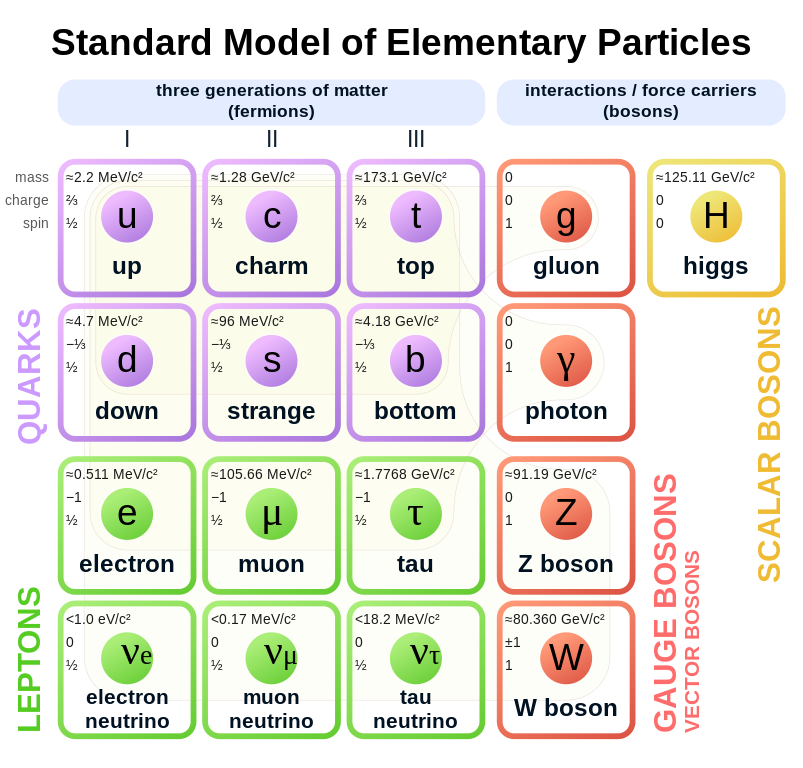
\includegraphics[width=0.8\textwidth]{Images/Theory/particlesSM.png} % TODO update to a more up to date. % TODO update the ref
    \caption[Particles in the SM]{Elementary particles of the Standard Model \cite{tableSMWiki}. Elementary fermions (quarks on top, lepton on the bottom) are listed in the three left columns and elementary bosons in the two right ones, the gauge bosons in the first column and the Higgs scalar boson in the last one. The mass, electrical charge, and spins of the particles are indicated.}
    \label{particlesSM}
\end{figure}

Particles are separated based on their intrinsic angular momentum or \textit{spin}, with half-spin particles following the Fermi-Dirac statistics called \textit{fermions}, and integer-spin particles called \textit{bosons} following the Bose-Einstein statistics. The elementary fermions are evenly split into 6 quarks and 6 leptons, with only the first generation of each being stable. The distinction between these two types stems from the different quantum numbers categorising them. Quarks carry a fractional electromagnetic charge as well as a colour charge making them sensitive to the strong interaction. On the contrary, leptons are colour-neutral and either have an electrical charge of -1$e^+$, in units of the anti-electron (positron) charge, or are neutral. The charged leptons include the electron $e^-$ - the lightest and only stable one -, the muon $\mu^-$, and the tau $\tau^-$. The neutral leptons are called neutrinos, with one neutrino $\nu_\ell$ associated per charged lepton $ell$, e.g., the electron-neutrino $\nu_e$. For the quarks, the electromagnetic charge is fractional, dividing them evenly between \textit{up}-type quarks with charge +$\frac{2}{3}$ consisting of the up $u$, charm $c$, and top $t$ flavours, and the \textit{down}-type quarks with charge -$\frac{1}{3}$ and the flavours down $d$, strange $s$, and bottom $b$. To every particle corresponds an \textit{anti}particle, with the same quantum numbers except for the electrical charge that changes sign. \\

The kinematics and dynamics of the fields representing the particles in the theory are expressed through a Lagrangian density $\mathcal{L}$, a spacetime discretisated element of the general Lagrangian. Symmetries of the Lagrangian density play an essential role as they define conserved quantities through Noether's theorem. The construction of the \gls{sm} Lagrangian id dictated by the expression of these symmetries to satisfy the experimentally observed conserved quantities, such as the electromagnetic charge. Two types of symmetries can be considered: global ones that are valid across spacetime and local ones, the so-called gauge symmetries valid for localised transformations. The \gls{sm} Lagrangian must satisfy the global Poincaré symmetry, encapsulating the symmetry required for special relativity, and a local non-Abelian $SU(3)_C \otimes SU(2)_L \otimes U(1)_Y$ gauge symmetry. Non-Abelian groups are such that their generators do not commute. The Lagrangian density of a field $\psi$ is a function of $\psi$ and its spacetime partial derivative $\partial_{\mu} \psi$, where $\mu$ indexes the time and space dimenions in the 4-vector formalism. The full \gls{sm} Lagrangian $\mathcal{L}_{\text{SM}}$ can be decomposed into 4 terms:
\begin{equation}\label{eq-SMGlobal}
    \mathcal{L}_{\text{SM}} = \mathcal{L}_{\text{EW}} + \mathcal{L}_{\text{QCD}} + \mathcal{L}_{\text{Higgs}} + \mathcal{L}_{\text{Yukawa}}.
\end{equation}
These different terms represent different effects encoded within the unified framework of the \gls{sm}. Three of the four known interactions of nature are encapuslated in the \gls{sm}: the strong, the electromagnetic, and the weak forces, with the gravitational force considered aside due to the weakness of its influence at sub-atomic scales. The mediators of the three included interactions are the gauge bosons, spin 1 particles with different properties arising from the nature of the interaction they carry. The electromagnetic and weak force have been successfully unified as a single \gls{ew} interaction, while the theory of the strong force is \gls{qcd}. One essential element in the \gls{sm} is the so-called Higgs interaction, a special force through which some gauge bosons acquire mass. This Higgs interaction is underpinned by a Higgs field, an excitation of which is called a Higgs boson $H$. Interactions between the Higgs field and quark can be introduced to assign masses to the latter through Yukawa couplings. The latter part of this thesis is dedicated to a measurement of such couplings to $b$- and $c$-quarks. The different interactions and their respective gauge bosons are further reviewed in this chapter.

\subsection{Quantum Electrodynamics}\label{subsec-QED}
\glsfirst{qed} is the theory underpinning the behaviour of free fermions and their electromagnetic interactions, for which the gauge carried are the photons. Fermions are represented by a Dirac spinor field $\psi(x)$ defined over spacetime $x$. The Dirac equation of quantum mechanics is a first order partial derivative equation modelling the free dynamics of such a spin-$\frac{1}{2}$ fermion with:
\begin{equation}\label{eq-dirac}
    (i\gamma^{\mu} \partial_{\mu} - m) \psi = 0,
\end{equation}
where $\gamma^{\mu}$ are the Dirac $\gamma$-matrices generalising the Pauli spin matrices to spacetime dimension, and the Einstein notation is adopted, summing over indices repeated as covariant and contravariant. For clarity, any contraction $\gamma^{\mu} \partial_{\mu}$ is denoted as $\cancel{\partial}$. A Lagragian density can be constructed to result in the dynamics described by Equation \ref{eq-dirac} through application of Euler-Lagrange:
\begin{equation}\label{eq-diracLag}
   \mathcal{L}_{\text{Dirac}} = \bar{\psi} (i \cancel{\partial}- m) \psi,
\end{equation}
Such a Lagrangian models the free dynamics of any spin-$\frac{1}{2}$ fermion, such as an electron $e^-$. Electrons have a $q = -1$ charge that is conserved by every known interactions. This conservations must be the result of a symmetry: the Dirac Lagrangian must be made invariant under a local gauge $U(1)$ transformation:
\begin{equation}\label{eq-GaugeU1}
    \psi \rightarrow \psi' = e^{-iq\alpha(x)} \psi ,
\end{equation}
which corresponds to a rotation in the complex spacetime by a phase $q\alpha(x)$. For the Lagrangian of Equation \ref{eq-diracLag} to satisfy this symmetry, the partial derivative $\partial_{\mu}$ must be replaced by the \textit{gauge covriant derivative $D_{\mu}$}:
\begin{equation}\label{eq-GaugeU1}
    \partial_{\mu} \rightarrow \partial_{\mu} + iqA_{\mu},
\end{equation}
where a new vector field $A\mu$ is introduced and required to transform under the $U(1)$ symmetry as $A_{\mu} \rightarrow A'_{\mu} = A_{\mu} + \partial_{\mu} \alpha(x)$. The elegance of this approach is the possibility to give this fauge field $A_{\mu}$ its own dynamic, modifying the Lagrangian of Equation \ref{eq-diracLag} into the \gls{qed} Lagrangian: \[ \mathcal{L}_{\text{QED}} = \bar{\psi} (i \cancel{\partial}- m) \psi + q \bar{\psi} \cancel{A} \psi - \frac{1}{4} F_{\mu\nu} F^{\mu\nu} \]
\begin{equation}
    \mathcal{L}_{\text{QED}} = \bar{\psi} (i \cancel{D}- m) \psi - \frac{1}{4} F_{\mu\nu} F^{\mu\nu}
\end{equation}
where $F_{\mu\nu} = \partial_{\mu} A_\nu - \partial_\nu A_{\mu} $ is the electromagnetic field tensor. The last term introduces a kinetic term for the gauge field and the interaction between the fermion $\psi$ and the gauge field $A$ is represented by the term combining them. In the present case, the charge $q$ is the conserved quantity of the gauge symmetry, which required the introduction of a new gauge field $A_\mu$ that can be interpreted as the photon field and given the dynamic of the electromagnetic interaction through $F_{\mu\nu}$. Fermionic fields can be introduced in this approach for the different known fermions, $\psi_e$, $\psi_{\mu}$, $\psi_u$, $\psi_c$, etc. Their interactions with $A_\mu$ defining each time a unique conserved electromagnetic charge $q_e$, $q_{\mu}$, $q_u$, $q_c$, etc.  This procedure is however general: the gauge invariance of a Lagrangian introduces a spin-1 gauge vector boson. The required $U(1)$ invariance forbids the presence of mass terms of the form $m^2 A^{\mu} A_{\mu}$, seemingly condemning the gauge bosons to be massless. 

\subsection{Electroweak Sector}
The weak force is described by two massive gauge vector bosons: the $W^{\pm}$ of mass $m_W \approx 80.4$ GeV\footnote{The unit system adopted throughtout this thesis is to set the speed of light in vacuum $c$ at 1, leading to masses expressed in GeV. To convert to mass units, one simply needs to divide by the standard unit $c^2$.} and the $Z^0$ of mass $m_Z \approx 91.2$ GeV. This apparent contradiction with the massless requirements of a $U(1)$ symmetry is elegantly solved by the Brout-Englert-Higgs mechanism \cite{Englert:1964et,  PhysRevLett.13.508}. This mechanism, described in the next section, is applied to a joint expression of the electromagnetic and weak forces known as \glsfirst{ew} theory in the Glashow-Weinberg-Salam (GWS) model \cite{GLASHOW1961579, PhysRevLett.19.1264, Salam:1968rm}. The fundamental symmetry group the theory is built upon is the non-Abelian $SU(2)_L \otimes U(1)_Y$, where $SU(2)_L$ is the weak isospin and $U(1)_Y$ the weak hypercharge. A local $SU(2)$ transformation acts as:
\begin{equation}\label{eq-GaugeSU2}
    \psi \rightarrow \psi' = e^{i g \alpha^a(x) T^a } \psi,
\end{equation}
where $T^a = \sigma^a / 2$ are the generators of the $SU(2)_L$ group, built from the $\sigma^a$ Pauli matrices ($a = 1, 2, 3)$. Each generator corresponds to a gauge field. The gauge field linked to $SU(2)_L$ leads to covariant derivative, simularly to Equation \ref{eq-GaugeSU2}, to ensure gauge invariance as expressed by
\begin{equation}\label{eq-GaugeSU2}
   D_{\mu}  = \partial_{\mu} + igT_a W_{\mu}^a,
\end{equation}
with three gauge fields $W_{\mu}^1$, $W_{\mu}^2$, $W_{\mu}^3$ with interaction strength $g$. The particularity of the weak interaction is that the charged current interactions described by the symmetry group $SU(2)_L$ only apply to left-handed $L$ particles states and not the right-handed $R$. Consequently, fermionic fields are decomposed into \[\psi = \psi_L + \psi_R\] with left-and right-handed particles represented by isospin doublets. The weak isospin $I_W$ charge of left-handed particles is $I_W = 1/2$, with a third component $I_W^3 = \pm  1/2$. For the right-handed part, $I_W = 0$ with $I_W^3 = 0$, decoupling it from the gauge bosons $W_{\mu}^a$. Physically, the observed weak charge current interaction corresponding to the $W^{\pm}$ bosons are the linear combinations of gauge fields:
\begin{equation}
    W_{\mu}^{\pm} = \frac{1}{\sqrt{2}} \left(W_{\mu}^{1} \mp W_{\mu}^{2} \right)
\end{equation}
These $W$ bosons only couple to left-handed particles, but an experimentally observed $Z$ boson couples to both left- and right-handed particles. This represented by the additional $U(1)_Y$ symmetry of the weak interaction in the \gls{sm}, with weak hypercharge $Y$, coupling $g'$, and an additional gauge field $B_{\mu}$. The weak hypercharge is \[Y = 2 (Q - I_W^3),\] with $Q$ the electromagnetic charge. The total covariant derivative of the electroweak sector of the \gls{sm} is therefore expressed by the GSM model as 
\begin{equation}\label{eq-GaugeEW}
    D_{\mu}  = \partial_{\mu} + ig T_a W_{\mu}^a + ig' \frac{Y}{2} B_{\mu}. % TODO should these be the g and g
\end{equation}
where $W_{\mu}^a$ and $B_{\mu}$ are respectively the $SU(2)_L$ and $U(1)_Y$ gauge bosons. The GSM model re-expresses the electromagnetic photonic field $A_\mu$ and the $Z$-boson field $Z_{\mu}$ as a linear combination of $B_{\mu}$ and $W_{\mu}^3$ depending on the \textit{weak mixing angle} $\theta_W$, a fundamental parameter of the \gls{sm} such that:
\begin{equation}\label{eq-weakmixangle}
    \cos\theta_W = \frac{g}{\sqrt{g^2 +g'^2}}.
\end{equation}
This establishes a connexion between the coupling strengths of the weak interaction and the electromagnetic interaction coupling $e$ as \[e = g \sin \theta_W = g' \sin\theta_W \cos\theta_W.\] The intrinsic strength of the weak interactions is indeed of similar ordar to that of the electromagnetic interaction but is weak in apparance due to its gauge bosons being massive. The weak force is the only known fundamental interaction to violate parity conservation. Neutrinos can only interact throught the weak force, which can itself only apply to left-handed particles. As a result, there are no right-handed neutrinos in the \gls{sm}. \\

A significant achievement of modern particle physics is the unification of interactions that are perceived as different at low-energies. The problem of the measured mass of the vector gauge bosons remains. Additionaly, the split of fermionic fields into a left- and right-handed componets lead the mass terms to violate the gauge invariance. Both issues are resolved by the mechanisn of the Brout-Englert-Higgs and Yukawa interactions, introduced in the next sections.

\subsection{The Brout-Englert-Higgs Mechanism}
The Brout-Englert-Higgs mechanism, abbreviated $BEH$ henceforth, offers a solution to introduce mass terms to the gauge fields $W_{\mu}^{\pm}$ and $Z_{\mu}$ \cite{Englert:1964et,  PhysRevLett.13.508}. It introduces a new scalar Higgs field, permeating the Universe. The field is mathematically defined as a weak isospin doublet, with a neutral component $\phi^0$ and a charged one $\phi^+$. They are jointly expressed as complex scalar field with 4 degrees of freedom:
\begin{equation}
\phi = \begin{pmatrix}
    \phi^+\\ 
    \phi^0
\end{pmatrix} = \frac{1}{2} \begin{pmatrix}
    \phi_1 + i\phi_2 \\ 
    \phi_3 + i\phi_4
\end{pmatrix}
\end{equation}
This complex scalar field is made to interact with the electroweak gauge fields as 
\begin{equation}\label{eq-HiggsLag}
    \mathcal{L_{\text{Higgs}}} = (D_{\mu}\phi)^{\dagger} (D^{\mu}\phi) - V(\phi),
 \end{equation}
where the first term described the kinetic of the $\phi$ and the second term is the Higgs potential energy:
\begin{equation}\label{eq-HiggsLag}
 V(\phi) = - \mu^2  \phi^{\dagger} \phi + \lambda (\phi^{\dagger} \phi)^2.
\end{equation}
where the expression of this potential is constrained by the need for the theory to be renormalisable. Two scalars constants govern the Higgs potential: $\mu$ and $\lambda$ describing, respectively, the quadratic and quartic interaction of the complex Higgs field $\phi$. The former manifests the interaction with the gauge bosons, while the latter introduces self-interactions. The minimum of this potential corresponds to the vacuum state. The requirement that the vacuum be stable demands $\lambda > 0$. For a positive $\mu^2 > 0$, a degenerate minimum is found at field values such that
\begin{equation}\label{eq-HiggsLag}
    \phi^{\dagger} \phi  = \frac{1}{2} (\phi_1^2 + \phi_2^2 + \phi_3^2 + \phi_4^2) = \frac{- \mu^2}{2\lambda} = \frac{v^2}{2}
\end{equation}
introducing in the last equality the so-called \textit{vacuum expectation value} $v = \sqrt{\frac{|\mu^2|}{\lambda}}$ of the field $\phi$. This infinite degeneracy of the Higgs potential minimum states underlines a special $SU(2)$ symmetry such that $\phi^{\dagger} \phi = v^2/2$. Through \textit{spontaneous symmetry breaking}, the BEH mechanism crumbles this degeneracy into one single vacuum state, typically chosen by setting the components $\phi_1 = \phi_2 = \phi_4 = 0$ and $\phi_3 = v$ so that the vacuum expactation is simply
\begin{equation}
\langle0|\phi|0 \rangle = \frac{1}{\sqrt{2}} \begin{pmatrix}
        0\\ 
        v
    \end{pmatrix}.
\end{equation}
The breaking of the symmetry enforces \[ SU(2)_L \otimes U(1)_Y \rightarrow U(1)_Q,\] with the final vacuum state correctly set as chargeless. Expanding the full field dynamic around the chosen vacuum state with a particular gauge choice to absord unphysical Goldstone fields into the vector fields called \textit{unitarity gauge} \cite{PhysRevD.7.1068}, the expansion can be simplified to 
\begin{equation}
    \phi = \frac{1}{\sqrt{2}} \begin{pmatrix}
            0\\ 
            v + h(x)
        \end{pmatrix},
\end{equation}
where $h$ is the real neutral Higgs scalar field. Introducing this expression into the Higgs Lagrangian of Equation~\ref{eq-HiggsLag} gives
\begin{equation}\label{eq-fullHiggs}
    \begin{split}
        \mathcal{L}_{\text{Higgs}} = & \,\frac{1}{2} (\partial_\mu h)(\partial^\mu h) + \frac{\mu^2}{2}(v+h)^2  - \frac{\lambda}{16}(v+h)^4 \\
        &+ \frac{1}{4} g^2 (W_{\mu}^+W^{\mu-})(v+h)^2 + \frac{g^2_W + {g'}^2}{8}(Z_{\mu}Z^{\mu})(v+h)^2 
    \end{split}
\end{equation}
where one can clearly identify mass terms for the physical gauge fields $W_{\mu}^{\pm}$ and $Z_\mu$ in the last line, but not for $A_{\mu}$ as required from observations that photons are massless. The vector gauge bosons masses are:
\begin{equation}
    m_W = \frac{v}{2} g , \, m_Z = \frac{v}{2}\sqrt{g^2 +g'^2} 
\end{equation}
or equivalenty expressing the mass of the $Z$-boson in terms of the $W$-boson mass \[m_Z = \frac{m_W}{\cos\theta_W}.\] The Higgs field is massive\footnote{This requires to isolate the terms in $h^2$ in Equation \ref{eq-fullHiggs}.} with mass \[m_H = \sqrt{2|\mu^2|}.\]
The BEH mechanism elegantly assigns mass to the gauge vector boson, with the photon remaining massless and the addition of the Higgs boson $H$ as a massive elementary particle. Furthermore, the introduction of the related Higgs field permits the expression of mass terms for the fermions in the standard model, as explained in Section~\ref{subset-yukint} on Yukawa interactions. 

\subsection{Quantum Chromodynamics}
The strong interaction is described by the theory of \textit{\glsfirst{qcd}}, underpinned by an $SU(3)_C$ symmetry with conserved quantum number called \textit{colour}. The only particles having a colour charge in the \gls{sm} are quarks and gluons $g$, the gauge mediators of the strong interactions. There are three colour charges typically labelled \textit{red}, \textit{blue}, and \textit{green}, each coming into its direct or anti-colour (e.g., anti-red). Quarks carry one such charge and gluons two. Similarly to the electroweak sector, the symmetry leads to a covariant derivative under the $SU(3)_C$ group of
\begin{equation}\label{eq-GaugeQCD}
    D_{\mu}  = \partial_{\mu} + ig_s \lambda_a G_{\mu}^a. % TODO should these be the g and g
\end{equation}
where the coupling constant $g_s$ of the strong interaction is often re-expressed as $\alpha_s = \frac{g_s}{4\pi}$, and the generator of the $SU(3)_C$ group are the set of eight $\lambda_a$ Gell-Mann matrices. The gauge field introduced here are the $G_{\mu}^a$ corresponding to the associate mediator of the strong field: the gluons $g$. Gluons carry 2 colour charges, leading to the 8 Gell-Mann matrices $\lambda^a$ and 8 gauge vector fields $G_{\mu}^a$. The generators of the $SU(3)_C$ group do not commutate: \[ [\lambda^a, \lambda^b] = i f^{abc} \lambda^c,\] where $f^{abc}$ are the $SU(3)_C$ structure constants.  Similarly to the electromagnetic strength tensor, strength tensors are built from the gluon fields as \[G_{\mu\nu}^a = \partial_{\mu} G_{\nu}^a   - \partial_{\nu} G_{\mu}^a - g_s f^{abc} G_{\mu}^b G_{\nu}^c.\]
This leads to a total \gls{qcd} Lagrangian of:
\begin{equation}\label{eq-QCDLag}
    \mathcal{L}_{\text{QCD}} = -\frac{1}{4} G_{\mu\nu}^a G^{\mu\nu}_a + \sum_{k} \bar{\psi}_k (i \cancel{D} - m_k) \psi_k,
\end{equation}
where $\psi_k$ are the six quarks fields, one per flavour, transforming as an $SU(3)_C$ triplet with one component per colour quantum number. Cubic and quartir terms in the gluon gauge fields $G_{\mu}^a$ are included, introducing self interaction of gluons. The non-commutation of the $SU(3)_C$ generators means the $SU(3)_C$ part of the \gls{sm} is non-Abelian group, and therefore a case of a Yang-Mills theory requiring this self-interacting gauge fields \cite{PhysRev.96.191}. \\

Like every coupling constant, $\alpha_s$ varies with energy. At low energies, the interaction is so strong that perturbative calculation breaks and the behaviour of \textit{colour confinement} is observed: any attempt to isolate a quark requires so much energy that a quark-antiquark pair is spontaneously produced. The strength of this interaction explains it short propagation distance despite the fact its gluonic mediatiors are massless. At higher energies $\sim 100$ GeV, asympotic freedom and perturbative calculations are possible thanks to the smallness of the coupling strength. This typically requires higher-order corrections for calculation to converge, with some terms, such as quark self-energy loops, diverging to infinity. This type of diverge is  called \textit{ultraviolet divergence}, and it is fixed by renormalising fields and parameters so that the divergence are absorbed away. This correction requires two parameters to arbitrarily define the scale of the process: the \textit{renormalisation scale} $\mu_R$ and \textit{factorisation scale} $\mu_F$ \cite{collins2004factorization}. The former is introduced to deal with ultraviolet divergences in the running of $\alpha_s$. The latter addresses the so-called \textit{infrared divergences} due to massless particles radiating further massless particles at low-energies by entering the parton distribution and fragmentation functions, introduced latter in this chapter.\\

Quarks must combine to form colour-less aggregate of matters called hadrons, with either a 2-quark system combining a quark and an antiquark into a \textit{meson}, or a 3-quark system forming a \textit{baryon} of which the proton ($uud$, $q_p = +1$) and the neutrons ($udd$, $q_n = 0$) are prime examples. The content of hadrons are called partons. The process leading to the neutralisation of the colour-charge of an asymptotically freed quark is called \textit{hadronisation}.\\

\subsection{Yukawa Interactions}\label{subset-yukint}
In the \gls{qcd} Lagrangian of Equation~\ref{eq-QCDLag}, the introduction of the mass terms for the quarks breaks the gauge invariance of the theory to $SU(2)_L \otimes U(1)_Y$ and must be therefore further modified. The masses of all fermions can however be included in the \gls{sm} by introducing so-called Yukawa interactions between the Higgs and fermionic fields. Such terms are expressed as the following Lagrangian:
\begin{equation}\label{eq-YukLag}
    \mathcal{L}_{\text{Yukawa}} = - \frac{1}{\sqrt{2}} \sum_{f} 
    y_f \bar{\psi}_f (v + h) \psi_f,
\end{equation}
where $\psi_f$ are the fermionic fields and the fundamental \textit{Yukawa coupling} parameters $y_f = \sqrt{2} \frac{m_f}{v}$ for each flavour of fermion $f$ are introduced as coupling strengths. Picking the $v$ component in the sum in parenthesis gives a clear mass term to the fermion, with the $h$ terms leading to Higgs-fermion interactions. The vacuum expectation value plays the role of a mass scale setting, with Yukawa coupling refining the specific strength for each fermionic species. For the quark sector, a futher correction is required as the weak interaction eigenstate basis is different from the mass basis in which physical particles are detected. The transformation from the mass eigenstates basis is specified by the complex unitary \textit{\gls{ckm} matrix} \cite{Tanabashi:2018oca}:
\begin{equation}
    V_{CKM} = \begin{pmatrix}
            V_{ud} & V_{us} & V_{ub}\\ 
            V_{cd} & V_{cs} & V_{cb}\\ 
            V_{td} & V_{ts} & V_{tb}\\ 
        \end{pmatrix},
\end{equation}
where the probability of a transition $p \rightarrow q$ is given by the magnitude $|V_{pq}|^2$ of the associated element. Through this quark mixing matrix, weak charged currents interaction allows for flavour-changing processes through charged currents interactions. The matrix is almost diagonal, hence transitions between quarks of the same generation are preferred (e.g., $t \rightarrow b$ preferred over $t \rightarrow d$).

\subsection{Experimental Higgs Phenomenology}
The experimental process to observe the Higgs bosons at the \gls{lhc} is to collide two proton beams head-on, as described in Chapter~\ref{chapter-ATLAS}. The accelerator is primarily designed to achieve these measurements, targeting different production and decay channels. Protons are composite particules (hadrons) and, at high energies, the main \textit{hard-scattering} interaction is beteen components of the protons called \textit{partons}. These partons are primarily the \textit{valence} quarks ($uud$ for a proton) but also contribution from \textit{sea} quarks, as well as gluons and photons present within the hadron due to quantum interactions. In a $pp$ collision, two interacting partons $ab$ from within the protons undergo the main event $ab \rightarrow X$, with the activity from the rest of the protons assigned to the so-called \textit{\gls{ue}}. The cross-section for the global process $pp \rightarrow X$ is expressed using the factorisation theorem \cite{collins2004factorization}: 
\begin{equation}
\sigma_{pp\rightarrow X} \sum_{a,b} \int_0^1 dx_a \int_0^1 dx_b f_a(x_a, \mu_F) f_b(x_b, \mu_F) \int d\sigma_{ab\rightarrow X}\left(x_aP_a, x_bP_b, \mu_R, \mu_F \right),
\end{equation}
where $f_i(x_i, \mu_F)$ is the \textit{\gls{pdf}} giving the probability for the parton $i$ to undergo a hard scattering with momentum $p_i = x_i P_i$, where $x_i$ is the fraction of the proton momentum $P_i$, $\mu_F$ is the previously introduced factorisation scale, as the \gls{pdf} depend on the energy scale of the underlying process. The interaction is effectively split into two steps: picking up the interacting partons and their fraction of momentum, then considering the main $ab \rightarrow X$ event.\\

As introduces in the previous section, the Higgs couples to particles proportionally to their measured mass, which influences its production and decay modes. The leading order production modes of the Higgs boson are schematised in Figure \ref{fig:prodH}. At the \gls{lhc} with a centre of mass energy $\sqrt{s} = 13$ TeV and a Higgs boson mass $m_H = 125$ GeV, the main processes presented are by decreasing cross-sections: 
\begin{itemize}[leftmargin=*] % TODO check values % TODO check for qqH
    \item \textit{Gluon-gluon fusion $ggF$}: two gluons fuse into a quark loop with a radiated Higgs boson: $pp \rightarrow H$. The quarks in the loop must couple to the Higgs, hence top $t$-quarks are preferred, followed by bottom $b$-quarks. The cross-section for this process is $\sigma_{ggF} = 48.6 \pm 2.4$ pb \cite{LHCHiggsCrossSectionWorkingGroup:2016ypw}. This process is favoured thanks the large contributions of gluons to the protonic \gls{pdf}s.
    \item \textit{Vector boson fusion $VBF$}: two off-shell vector bosons $V$ ($W$ or $Z$) radiated from partonic quarks fuse to form a Higgs $pp \rightarrow qqH$, with cross-section $\sigma_{VBF} = 3.77 \pm 0.09$ pb \cite{LHCHiggsCrossSectionWorkingGroup:2016ypw}. The quarks leave a characteristic twin forward jets in the event.
    \item \textit{Associated production with a vector boson $VH$}: the Higgs boson is produced in association with a vector boson $V$ ($W$ or $Z$): $pp \rightarrow VH$. This process is studied in greater detail in Chapter~\ref{}, dedicated to an analysis of Higgs decaying to $b$- or $c$-quarks from this production mode. It has a cross-section of $\sigma_{VH} = 2.24 \pm 0.14$ pb \cite{LHCHiggsCrossSectionWorkingGroup:2016ypw}. Leptonic decays of the associated vector boson give clean event signatures.
    \item \textit{Associated production with a quark pair $q\bar{q}H$}: an ``open quark loop'' is produced from a pair of partonic gluons, with a Higgs radiated $pp \rightarrow q\bar{q}H$. The dominating contributions come from the $t\bar{t}H$ associated production with cross-section $\sigma_{VH} = 0.51 \pm 0.04$ pb, followed by the $b\bar{b}H$ \cite{LHCHiggsCrossSectionWorkingGroup:2016ypw}.
\end{itemize}

\begin{figure}[h!]
    \center
    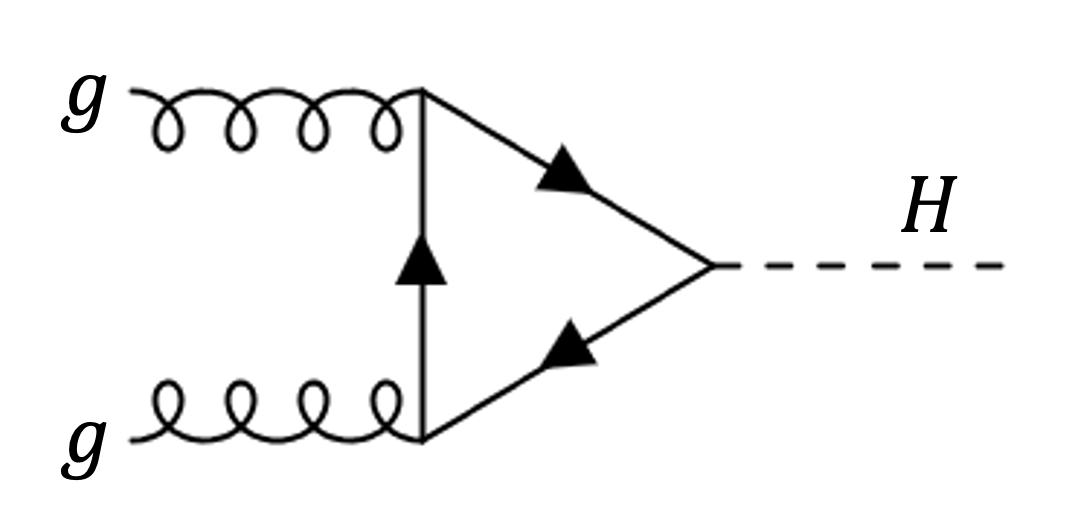
\includegraphics[width=0.24\textwidth]{Images/Theory/ggH.png}
    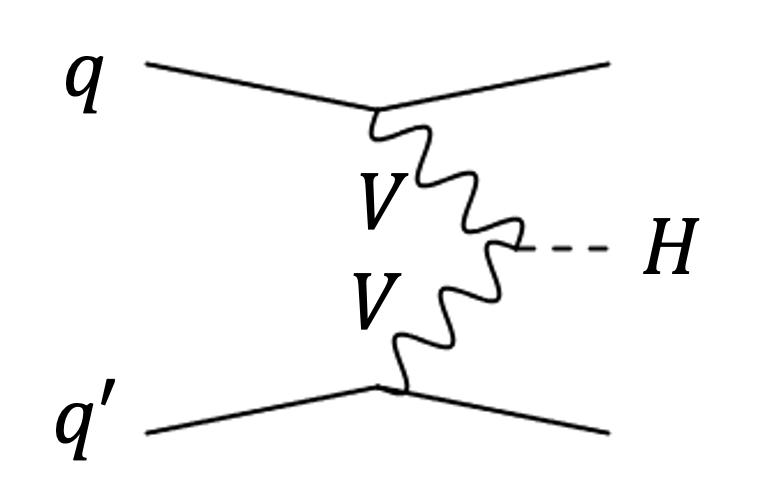
\includegraphics[width=0.24\textwidth]{Images/Theory/vvH.png}
    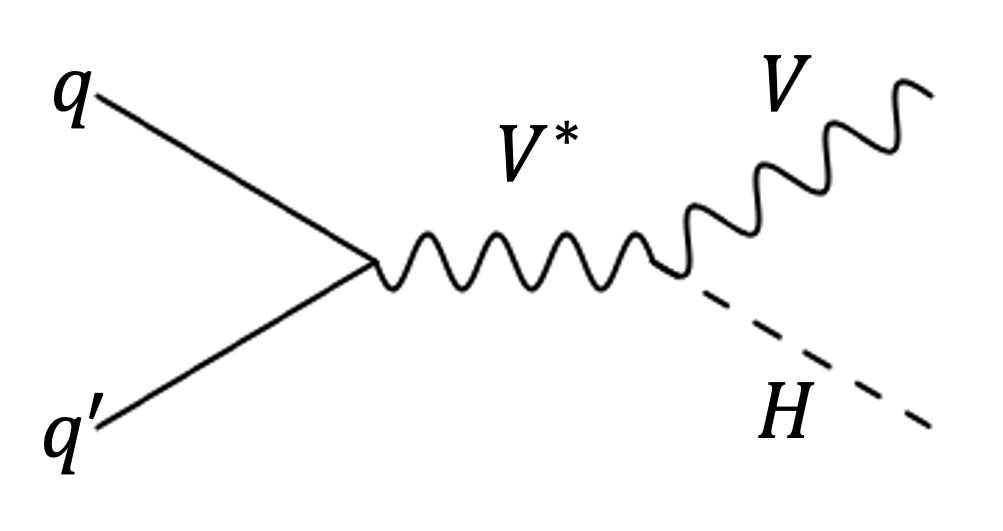
\includegraphics[width=0.24\textwidth]{Images/Theory/vh.png}
    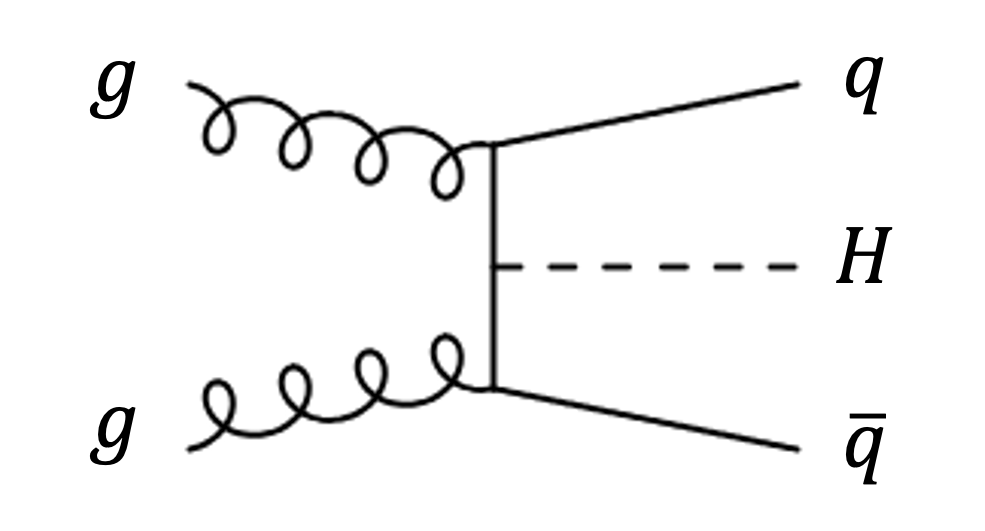
\includegraphics[width=0.24\textwidth]{Images/Theory/qqH.png}
    \caption{The leading order Feynman diagrams for Higgs production at the LHC, from left to right: gluon-gluon fusion ($ggF$), vector boson $V$ fusion ($VBF$), associated production with a vector boson ($VH$), and associated production with a $q\bar{q}$ pair ($q\bar{q}H$).}
    \label{fig:prodH}
\end{figure}

The dependency of the Higgs boson production from proton-proton collisions at $\sqrt{s} = 13$ TeV are represented in the left of Figure~\ref{fig:prodH} as a function of the Higgs boson mass $m_H$. The total width of the \gls{sm} Higgs boson is $\Gamma_H = 4$ MeV, implying a short lifetime of $\tau_H ~ 10^{-22}$ $s$ and restricting measurement to its decay products. The decay branching ratios are displayed in the right of the figure, with decays to heavier particles favoured due to the proportionality of the Higgs coupling strength to the mass. Decays to the massless gluons $g$ and photons $\gamma$ are possible thanks to intermediate quark loops, similarly to $ggF$. Relative decay rates are quantified by their branching ratio $BR$ as
\begin{equation}
    BR(H \rightarrow X) = \frac{\Gamma(H\rightarrow X)}{\Gamma_H}
\end{equation},
where the total Higgs width $\Gamma_H$ is the sum of all partial decay width $\Gamma(H\rightarrow X)$, for all possible $X$. The right of Figure~\ref{fig:prodH} displays the \gls{sm} Higgs branching ratio at $\sqrt{s} = 13$ TeV. The most likely Higgs decay mode is to a pair $b\bar{b}$ ($BR \approx 58$ \%), followed by the decay to a $WW$ pair ($BR \approx 21$ \%), and the $c\bar{c}$ decay branching ratio is 2.9\%. All the decay branching ratios are displayed in the right of the figure, with decays to heavier particles favoured due to the proportionality of the Higgs coupling strength to the mass. \\

\begin{figure}[h!]
    \center
    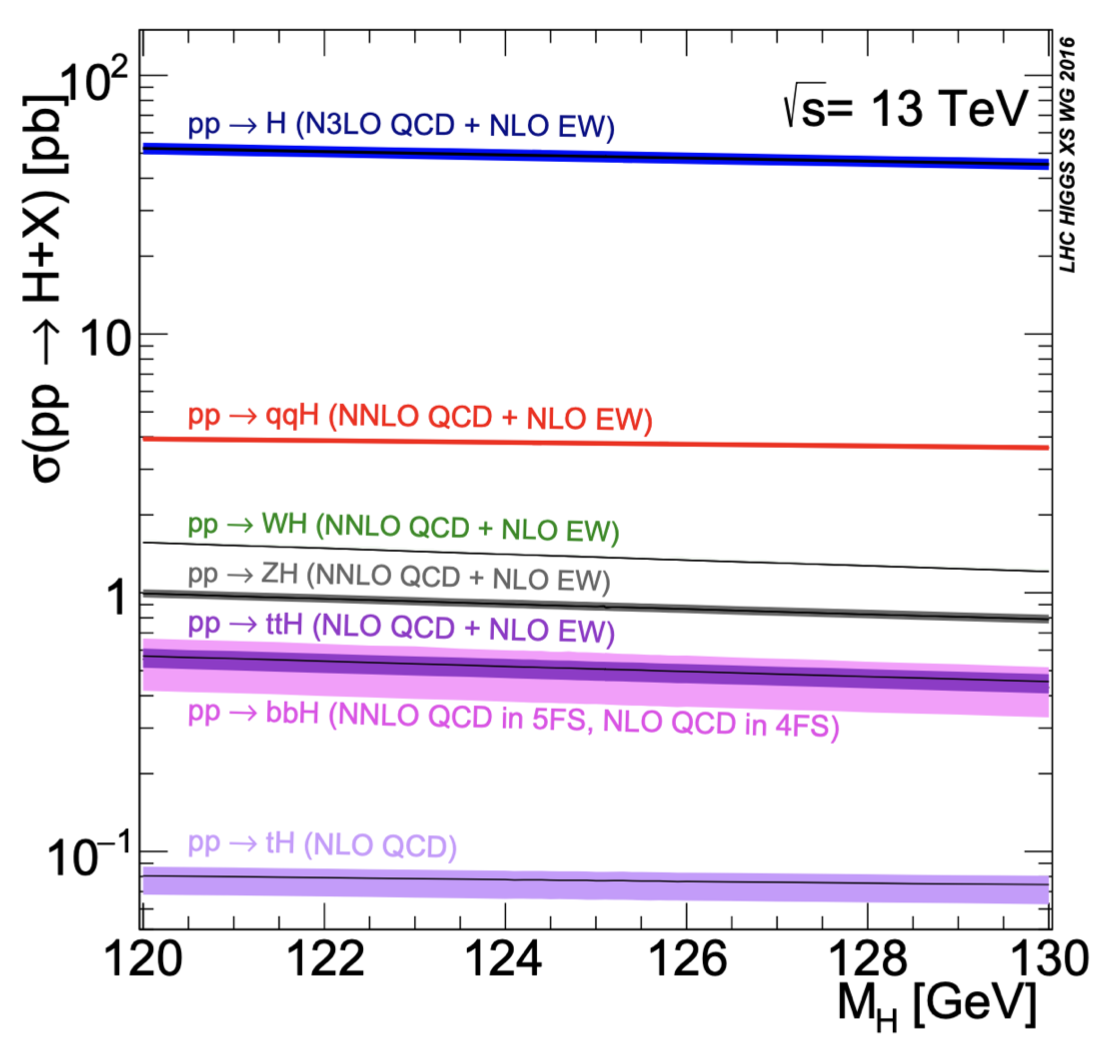
\includegraphics[width=0.48\textwidth]{Images/Theory/prodHiggs.png}
    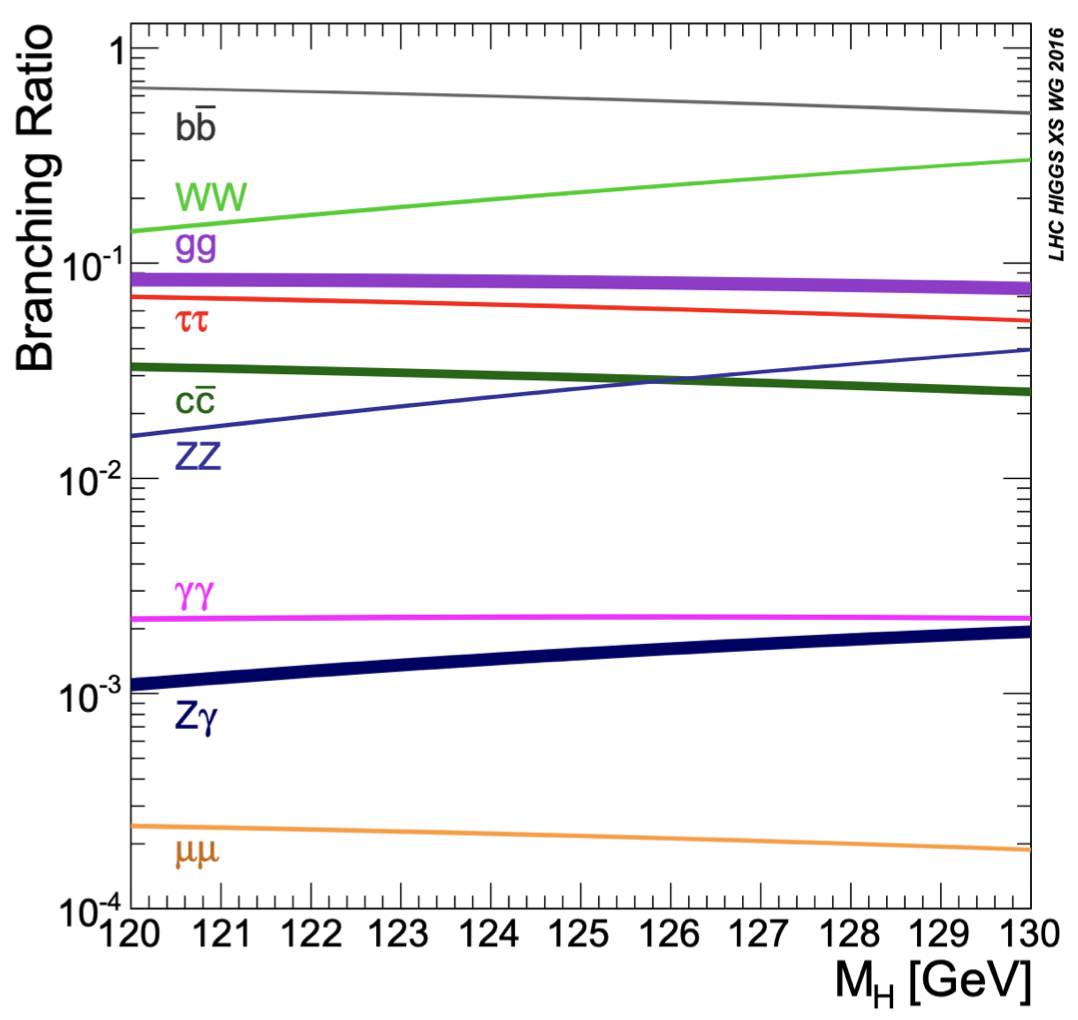
\includegraphics[width=0.48\textwidth]{Images/Theory/decayHiggs.png}
    \caption{The Standard Model production cross-sections from proton-proton collisions (left) and decay branching ratio (right) of the Higgs boson as a function of $m_H$, at $\sqrt{s} = 13$ TeV, from \cite{LHCHiggsCrossSectionWorkingGroup:2016ypw}.}
    \label{fig:prodH}
\end{figure}
\begin{figure}[h!]
    \hspace{-0.48cm}
    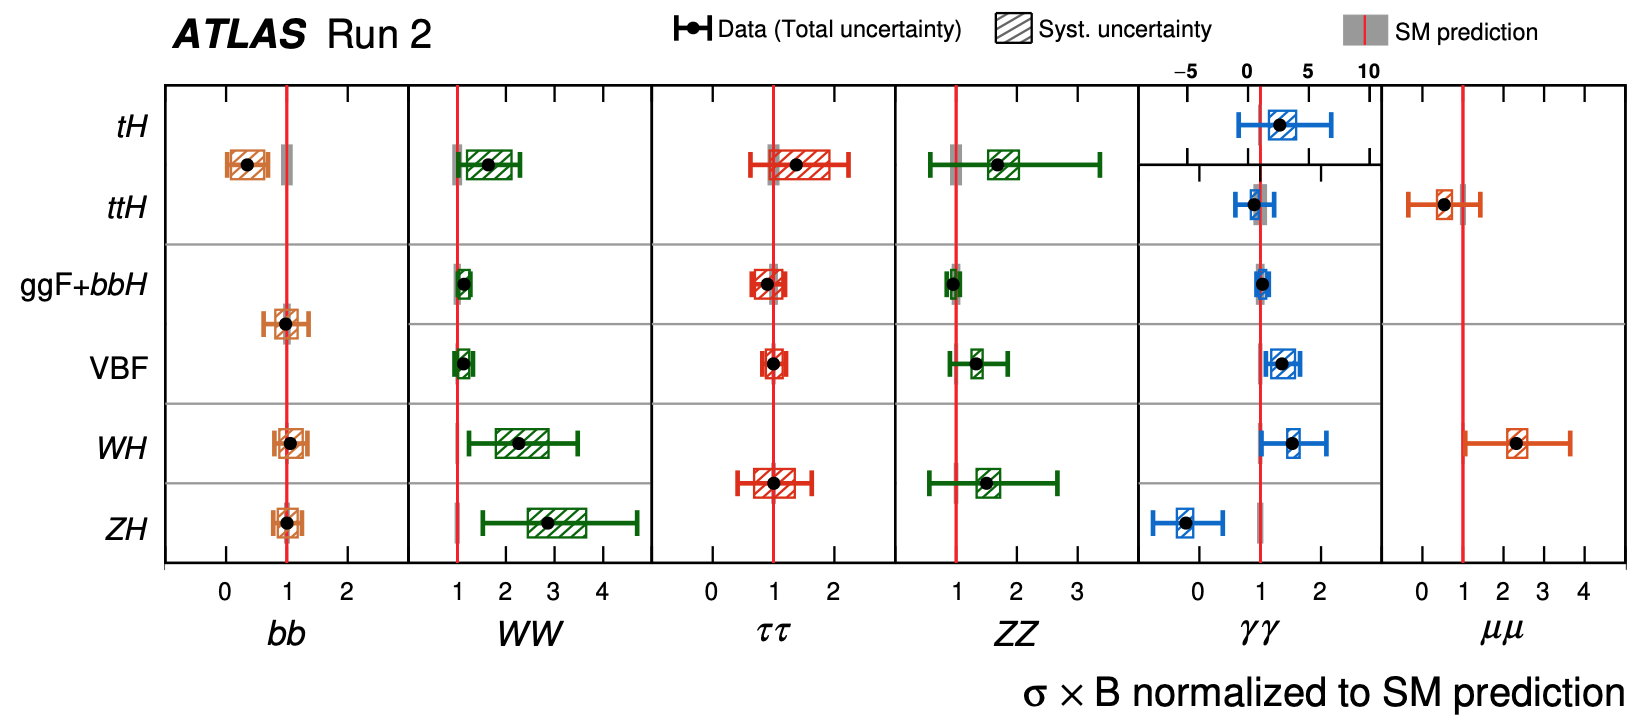
\includegraphics[width=\textwidth]{Images/Theory/allMesRun2.png}
    \caption{Ratio of observed to the SM predicted event rate for different combinations of Higgs boson production and decay mode, from \cite{ATLAS:2022vkf}. The horizontal bars denote the 68\% confidence interval, with grey bands showing the theory uncertainties on the SM cross-section $\times$ branching ratio predictions.}
    \label{fig:measprodH}
\end{figure}

The $W^+W^-$ and $ZZ$ decays can only be achieved by a virtual off-shell Higgs bosons. The fermionic decays are hard to observe due to the larger multi-jet background in a hadron collider. The vector bosons and di-photons leptonic decays benefit from advantageous experimental conditions, being easier to identify thanks to the presence of leptons and suffering from less background contamination. For these reasons, the ATLAS and CMS experiment both observed a particle of mass $m_H = 125$ GeV with the same properties as the Higgs boson in 2012 by combining the $H \rightarrow \gamma\gamma$, $H \rightarrow ZZ \rightarrow \ell^+\ell^-\ell'^+\ell'^-$, and $H \rightarrow W^+W^- \rightarrow \ell^+\ell^-\nu \bar{\nu}$ channels \cite{ATLAS:2012yve, CMS:2012qbp}. This opened the way to many additional Higgs measurements, with some of the most sensitive ones summarised in Figure \ref{fig:measprodH}. Decay modes to third generations particles ($t, b, \tau$) have been observed, with the sensitivity rising for the second generation ($\mu$). In all analyses, the Higgs boson is measured to be in remarkably consistent with the predictions from the \gls{sm} \cite{ATLAS:2022vkf}. 


\newpage
\chapter{\color{oxfordblue} The LHC \& ATLAS Experiment}\label{chapter-ATLAS}
\ChapFrame

\textit{
Modern particle physics explores the frontier of the technological reach of science. A remarkably complex infrastructure was necessary to probe physics at the required scale to discover the Higgs boson. The \gls{cern} hosts the largest and most powerful particle accelerator ever built: the \glsreset{lhc}\gls{lhc}. It has held this title since its construction concluded in 2008 \cite{LyndonEvans_2008}, and ranks among the most intricate machines ever created. Protons are accelerated to 99.9999991\% of the speed of light in a giant 27 km-long ring-shaped beamline, located 100 m below the surface of the French-Swiss border in the suburbs of Geneva. Superconducting magnets cooled with liquid helium to 1.9 $K$ steer this energetic beam thanks to powerful magnetic fields of 8.33 Tesla. The beams, composed of bunches of particles, collide at four precise interaction points where large detectors are built and operated by dedicated collaborations: ATLAS \cite{TheATLASCollaboration_2008}, CMS \cite{TheCMSCollaboration_2008}, ALICE \cite{TheALICECollaboration_2008}, and LHC$b$ \cite{TheLHCbCollaboration_2008}. The first two are multipurpose experiments with overlapping physics programs, while ALICE and LHC$b$ respectively study heavy-ion and heavy-flavour physics. This chapter describes the experimental setup of the \gls{lhc} and the ATLAS experiment, focusing on proton-proton collisions and introducing relevant elements for the work presented in this thesis.} 

\section{The Large Hadron Collider}\label{sec-LHC}
The last machine in the complex multi-stage accelerator system of CERN depicted in Figure \ref{fig-CernAccSys}, the \glsreset{lhc}\gls{lhc} is capable of frontally colliding proton or heavy ion beams packed into bunches. The beams collide at four interaction points, where dedicated experiments such as ATLAS measure the resulting physics signatures in large detectors designed for their specific physics programmes. The life of a proton beam starts in a bottle of ionised hydrogen ($H^-$) gas, the contents of which are passed through a linear accelerator called \textsc{linac} 4\footnote{\textsc{linac} 2 before 2020.} to reach an energy of 160 MeV \cite{Vretenar:2020quc}. After stripping the ionised hydrogen atoms of their two electrons to leave bare protons, the next acceleration stage happens in the Proton Synchrotron Booster (\textsc{booster}), bringing the beam's energy to 2 GeV \cite{Reich:1969fw}. The protons are then handed to increasingly larger synchrotrons: the Proton Synchrotron (\textsc{ps}) to reach an energy of 26 GeV \cite{CERNPS}, followed by the Super Proton Synchrotron (\textsc{sps}) to reach an energy of 450 GeV \cite{Synchrotron:1997188}. The beam is finally injected into the \gls{lhc} in two different beamlines circulating the proton in opposite directions \cite{Evans:2008zzb}. Superconducting dipole magnets generating an 8.33 T field steer the highly energetic beams, while complex geometries of magnets, such as quadrupoles and sextupoles, refine the bunch shape through focusing effects. Powerful radiofrequency cavities accelerate the protons to their final energy of 6.5 TeV each, giving a total $pp$ collision centre-of-mass energy of $\sqrt{s} = 13$ TeV in Run 2. 

\begin{figure}[!h]
  \centering
  \makebox[\textwidth][c]{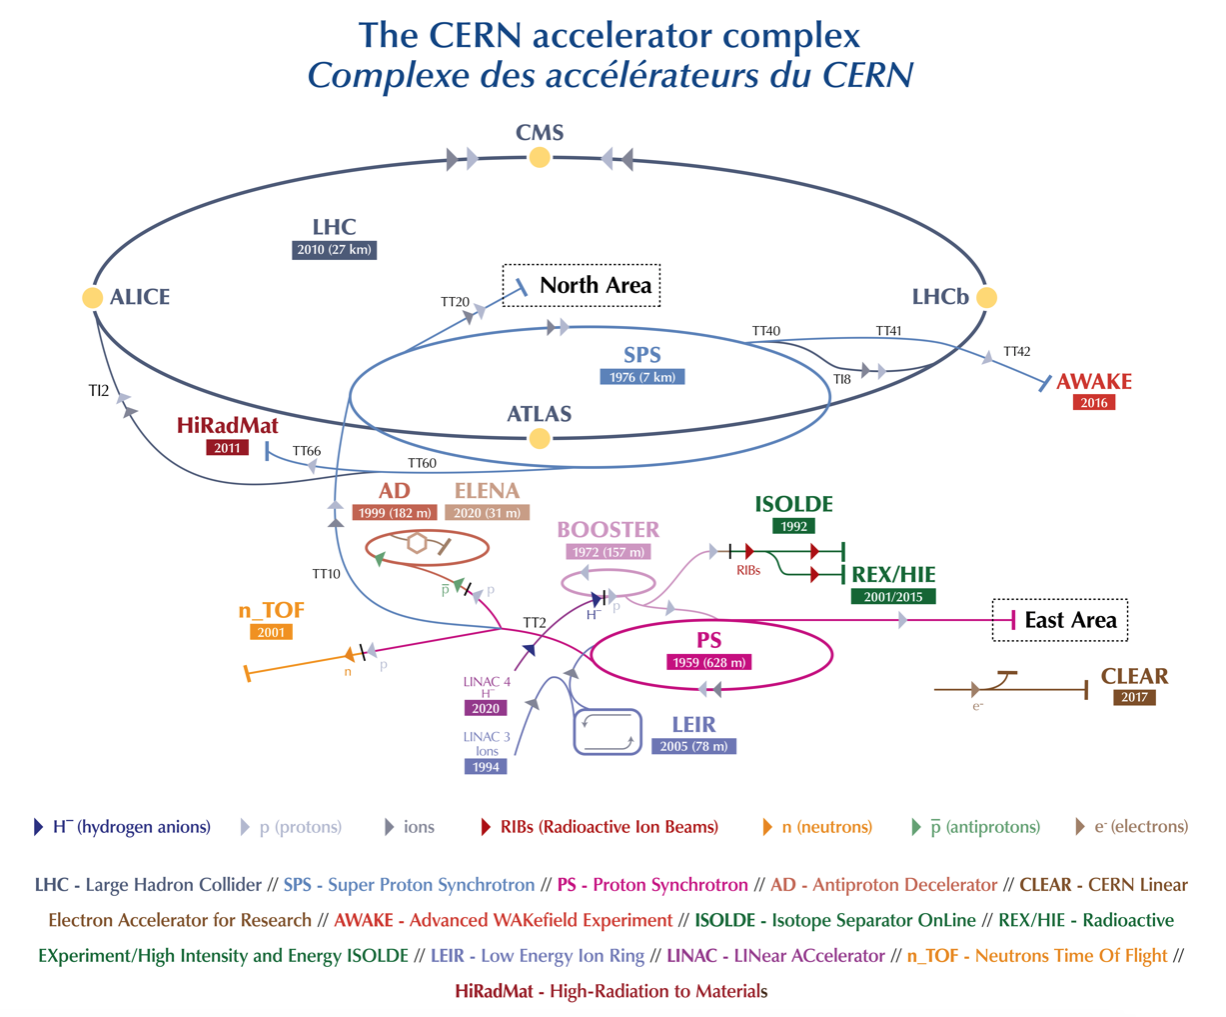
\includegraphics[width=1.05\textwidth]{Images/ATLAS/cernAcc}}
  \caption{The complete accelerator complex of CERN for Run 3 \cite{CERNAcc}.}
  \label{fig-CernAccSys}
\end{figure}

The operation of the \gls{lhc} is split into dedicated \textit{runs} of data-taking separated by \textit{shutdowns} to maintain or upgrade the infrastructure. Key metrics about these runs from the point of view of the ATLAS experiment are displayed in Table~\ref{tbl:LHCATLASperf}. Run 2 operated at a larger centre-of-mass energy ($\sqrt{s}$) and higher average instantaneous luminosity ($\mathcal{L}$) than Run 1.

%\vspace{-1cm}
\begin{table}[!htbp]
  \begin{center}
      \renewcommand{\arraystretch}{1.2}
    %\resizebox{0.99\textwidth}{!}{
      \begin{tabular}{cc|cccc} \hline \hline 
        & Year & $\sqrt{s}$ [TeV] & $\langle \mu \rangle$ &  Luminosity $\mathcal{L}$ [cm$^{-2}$s$^{-1}$] & $\int\mathcal{L}$ [fb$^{-1}$] \\ \hline
        Run 1 & 2010 - 2012 & 7-8    & 18 & 0.8 $\times$ $10^{34}$    & $26.4$ \\
        Run 2 & 2015 - 2018 & 13     & 34 & 1-2 $\times$ $10^{34}$  & $140.1$ \\
        Run 3 & 2022 - 2025 & 13.6     & 50 & 2 $\times$ $10^{33}$    & $65$ \\

        \hline\hline
      \end{tabular}
    %}
    \caption{Metrics on the accelerator performance of the LHC in the different runs of data taking. The reported values correspond to those recorded by the ATLAS experiment \cite{ATLAS:run1Lumi, ATLAS:2022hro, ATL-DAPR-PUB-2023-001}. Numbers for the ongoing Run 3 are preliminary, with the integrated luminosity listed considering events recorded until July 2023. The number of interactions per bunch crossing averaged over each run is displayed as $\langle \mu \rangle$.}
    \label{tbl:LHCATLASperf}
  \end{center}
\end{table}

The average instantaneous luminosity $\mathcal{L}$ measures the rate of data collection as
\begin{equation}
  \frac{dN}{dt} = \mathcal{L} \times \sigma,
\end{equation}
relating the event rate of a particular process to its cross section $\sigma$. The instantaneous luminosity is a machine parameter: it depends on the design and the operation of the accelerator. It is calculated from
\begin{equation}
  \mathcal{L} = \frac{N_1N_2N_bf}{4\pi\sigma_x\sigma_y}
\end{equation}
where $N_1$ and $N_2$ are the numbers of protons in each bunch, $N_b$ the number of bunches, $f$ is the collider revolution frequency, and $\sigma_x$ and $\sigma_y$ are the geometrical extensions of the beam density distribution in the $x$- and $y$-directions. The integrated luminosity $\int \mathcal{L}\, dt$ measures the number of events collected over a certain period, often expressed in units of inverse \textit{barn} b$^{-1}$, where 1 b $= 10^{-28}$ m$^{2}$. For Run 2, the total luminosity recorded by ATLAS corresponds to 140.1 $\pm$ 1.2 fb$^{-1}$, with a small uncertainty of 0.83\% \cite{ATLAS:2022hro} thanks to a complex measurement involving luminosity-dedicated detectors such as LUCID-2 \cite{Avoni_2018}. Figure \ref{fig-atlasLumiPileup} shows the cumulative distribution of the integrated luminosity during Run 2, along with another important machine parameter: the average number of interactions per bunch crossing $\langle \mu\rangle$.

\begin{figure}[!h]
  \centering
  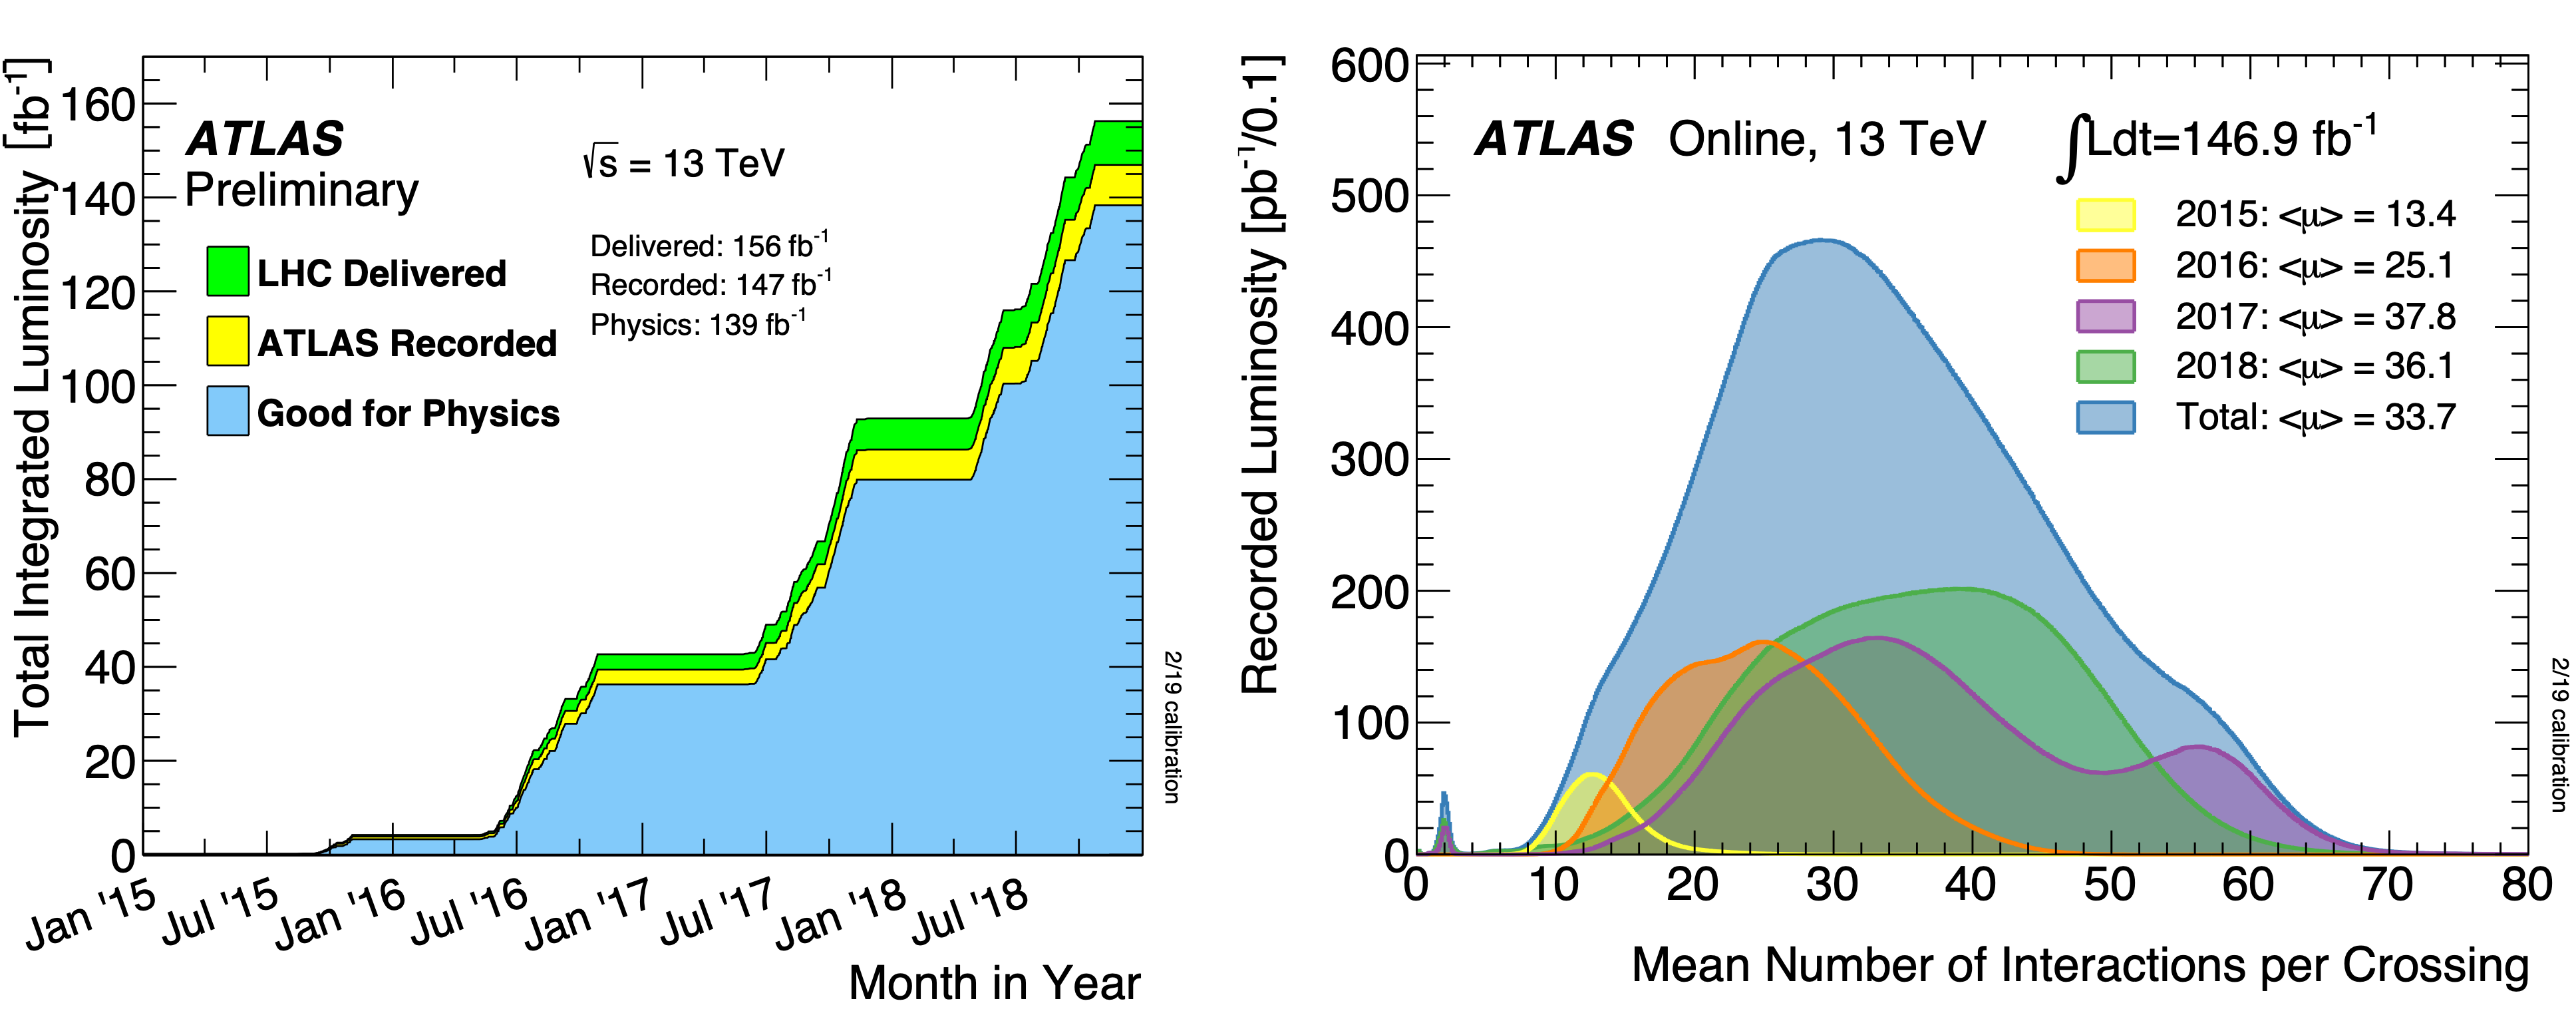
\includegraphics[width=\textwidth]{Images/ATLAS/recoATLAS.png}
  \caption{The cumulative integrated luminosity delivered, recorded, and useful for physics (left), and the average luminosity-weighted pile-up distribution (right) during Run 2 at ATLAS \cite{PubAtlasLumi}. The luminosities listed correspond to an early calculation that was refined in Ref. \cite{ATLAS:2022hro}.}
  \label{fig-atlasLumiPileup}
\end{figure}

The main event during the collisions of two protons is the inelastic hard scattering, where most of the energy transfer occurs. Other protons in the bunches can have softer interactions, leading to background activity referred to as \textit{\gls{pu}}. Two types of pile-up are distinguished: \textit{in-time \gls{pu}} when the soft interaction is from protons in the same bunch as those involved in the hard scattering, and \textit{out-of-time \gls{pu}} if the protons are from bunch-crossings just before or after the collision of interest. The \gls{lhc} separates bunches by a 25 ns delay, corresponding to a machine frequency of 40 MHz. To control the luminosity, the angle of attack of the beams is tweaked so that their geometrical overlap, measured by $\sigma_x$ and $\sigma_y$, at the point of impact is tunable. Having more head-on collisions leads to a larger overlap and higher luminosity but comes at the price of more \gls{pu}. 

\section{The ATLAS Detector}\label{sec-ATLASDet}
The ATLAS Collaboration maintains and operates the eponymous cylindrically shaped multi-layered detector, lying 100 m underground, with a length of 45 m and a diameter of 26 m \cite{TheATLASCollaboration_2008}, as presented in Figure~\ref{fig-AtlasDec}. The experiment is designed to probe a broad range of physical phenomena. Aiming to be as hermetic as possible, the detector wraps around the interaction point, with the barrel forming the central part of the cylinder and the endcaps closing the geometry at its extremities. Essential requirements in the technical design had to be met to manage the extreme event rate, requiring a fast response from radiation-hard sensors with state-of-the-art readout electronics in combination with good spatial and temporal resolution to disentangle the effect of pile-up.

\begin{figure}[!h]
\centering
\hspace{-1.25cm}
\makebox[\textwidth][c]{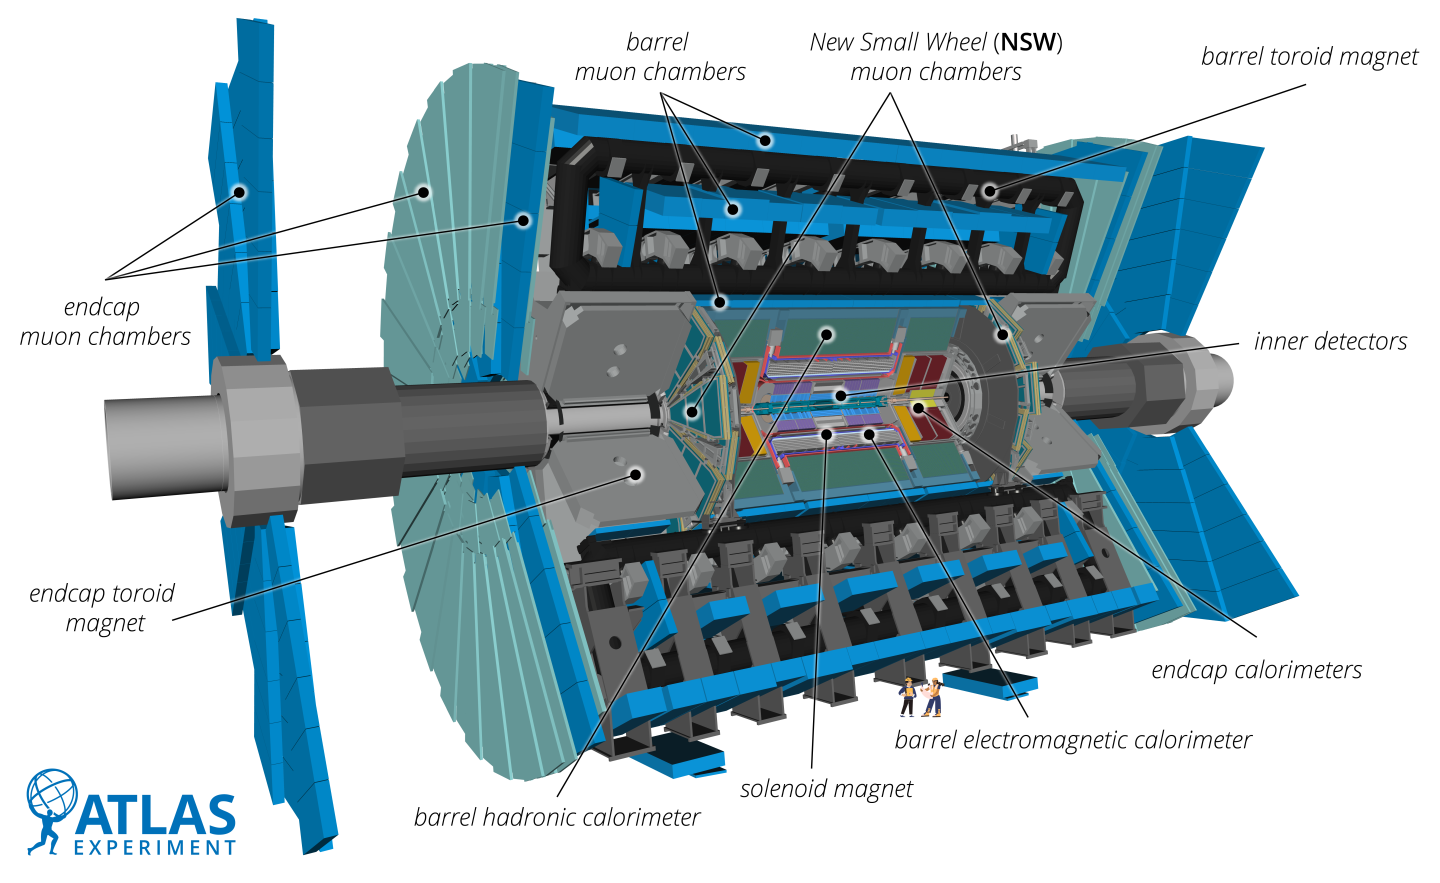
\includegraphics[width=1.08\textwidth]{Images/ATLAS/atlasDet.png}}
\caption{Cut-away view of the ATLAS detector \cite{ATLASschematics}.}
\label{fig-AtlasDec}
\end{figure}

\newpage
The coordinate system adopted in ATLAS is described in Figure \ref{fig-AtlasCoord}: the $x$-axis points to the centre of the \gls{lhc} ring, the $y$-axis points upwards, and the $z$-axis is in the longitudinal direction along the beamline, anti-clockwise when viewed from above. The azimuthal angle $\phi$ is defined in the transverse plane $x-y$, and the polar angle $\theta$ is measured upwards from the beam axis. The transverse momentum \pt\ of a particle is obtained from its momentum vector $\boldsymbol{p} = (p_x, p_y, p_z)$, of magnitude $p$, as \pt\ $= p \sin\theta = \sqrt{p_x^2 + p_y^2}$. This projection plays a crucial role, as the longitudinal component $p_z$ is not fully resolvable due to the openings for the beamline and the interacting partons carrying only a fraction of the original proton momenta. Therefore, only the transverse momentum can be reliably measured. Since the partons are mostly longitudinally boosted, the transverse momenta in an event are approximately balanced. The rapidity $y$ of a particle is expressed as 
\begin{equation}
  y = \frac{1}{2} \ln \left(\frac{E + p_z}{E - p_z}\right)
\end{equation}
with $E$ and $p_z$ the energy and longitudinal momentum of the particle. In the ultrarelativistic limit, when $p >> m$, the rest mass is negligible, and $E \approx p$. In this case, the rapidity $y$ is well approximated by the experimentally reconstructable pseudorapidity $\eta$:
\begin{equation}
  \eta = -\ln \left(\tan \frac{\theta}{2}\right).
\end{equation}
At high energies, $\Delta \eta$ becomes approximately invariant under Lorentz boosts along the $z$-axis. The pseudorapidity is often combined with the azimuthal angular aperture $\Delta \phi$ to define the angular separation $\Delta R$ between two objects as
\begin{equation}\label{eq-def-deltaR}
  \Delta R = \sqrt{\Delta \phi^2 + \Delta \eta^2} =  \sqrt{\Delta (\phi_2 - \phi_1)^2 + \Delta (\eta_2 - \eta_1)^2}.
\end{equation}

\begin{figure}[!h]
  \centering
  %\hspace{+0.5cm}
  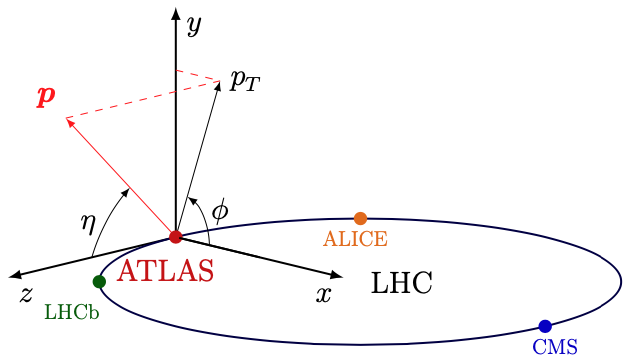
\includegraphics[width=0.6\textwidth]{Images/ATLAS/atlasCoor.png}
  \caption{The ATLAS coordinate system \cite{Strong:2020mge}.}
  \label{fig-AtlasCoord}
\end{figure}

As depicted in Figure~\ref{fig-AtlasDec}, ATLAS is composed of many subdetectors measuring information in the range $|\eta|<  2.5$, with some specialised subdetectors such as the calorimeters extending further. An essential feature of the detector is its magnetic fields. In ATLAS, they are provided by four superconducting magnets: the \textit{Central Solenoid}, which generates a 2 T axial magnetic field used by the central trackers, and a tangential magnetic field of about 1 T at the muon detectors, achieved by the \textit{Barrel Toroid} and the two \textit{Endcap Toroids}. A $q$-charged particle of momentum $p$ is deflected by a magnetic field $B$ due to the Lorentz force, leading to a relation between the radius of curvature $R$ of the trajectory and the momentum $p$ such that 
\begin{equation}
  p_{\perp} = 0.3 \, qBR \, [\text{GeV}/c],
\end{equation}
where $p_{\perp}$ is the magnitude of the momentum perpendicular to the magnetic field $\boldsymbol{B}$, and $q$ is expressed in the unit of proton charge. Therefore, the component of the momentum transverse to the magnitude $B$ can be inferred by measuring the curvature. Higher magnetic fields induce larger curvature, simplifying the measurement of $R$ and improving the resolution of $p_{\perp}$. \\ 

The rest of this chapter reviews the different subdetectors of ATLAS and introduces some common reconstruction methods that are relevant to the work presented in this thesis. 

\subsection{The Inner Detector Tracker}
The detector placed closest to the beam crossing point is the \textit{\gls{id}} \cite{CERN-LHCC-97-016}. This tracker, covering the range $|\eta| < 2.5$ in a radius of 3 cm to 1 m, is designed to record localised energy deposits called \textit{hits} in silicon semiconductors or straw tubes from the passage of charged particles. Subsequently, the trajectories or \textit{tracks} of these particles can be reconstructed by combining these signatures. The powerful 2 T magnetic field of the Central Solenoid enables this detector to measure both the charge and the momentum of charged particles. The \gls{id} combines three subsystems, represented in Figure \ref{fig-AtlasDecID}. 

\begin{figure}[!h]
  \centering
  \hspace{-1.25cm}
  \makebox[\textwidth][c]{\includegraphics[width=1.1\textwidth]{Images/ATLAS/ATLASinDecComb.png}}
  \caption{The Inner Detector of ATLAS \cite{ATLASschematics}.}
  \label{fig-AtlasDecID}
\end{figure}

First, the high-granularity \textit{Pixel Detector} covers the innermost region with three barrel and three endcap layers, for a total of 80 million sensitive semiconductor pixels \cite{CERN-LHCC-97-016, Potamianos:2015lar}. During Run 2, an additional \textit{\gls{ibl}} with 12 million pixels was added at a radius of 33 mm \cite{Capeans:1291633}. This detector gives robust and precise tracking performance and plays a major role in flavour tagging, as described in Chapter~\ref{chap-ftag}. The pixel dimensions range from 50 $\times$ 400 $\mu$m$^2$ in the Pixel Detector to 50 $\times$ 250 $\mu$m$^2$ in the \gls{ibl}, where the smaller dimension is used for the $R\phi$ measurement. The geometrical position resolution delivered is of 10 $\mu$m (67 $\mu$m) in the transverse $R\phi$ plane ($z$-direction) \cite{Pernegger_2015, ATL-INDET-PUB-2016-001}. \\

The \textit{\gls{sct}} is the next detector, constructed by arranging pairs of silicon microstrips layers into modules assembled into 4 concentric barrel layers and 9 disks in each endcap \cite{AHMAD200798, CERN-LHCC-2017-005}. The resolution is of 17 $\mu$m in $R\phi$ and 580 $\mu$m in $z$ \cite{ATLASSCT}. \\

The final system is the \textit{\gls{trt}}, a gas-based straw-tube tracker aiding track reconstruction by delivering numerous hits \cite{TheATLASTRTcollaboration_2008}. Approximately 300,000 drift tubes of a 4 mm diameter filled with a mixture of argon and xenon are arranged along the beamline in the barrel and radially in the endcaps. Each tube is fitted with a conducting wire at its centre and the surface is electrically charged, so that the passage of a charged particle ionises the gas leading to a measurable signal. Polyethylene is placed between the tubes to encourage the emission of transition radiations from relativistic particles proportionally to their Lorentz boost $\gamma \sim E / m$. The \gls{trt} is used for both tracking and electron and pion identification, by reconstructing the mass of the charged particles from the amount of $\gamma$-radiation. For tracking, the position resolution is 130 $\mu$m in the $R\phi$ plane for the barrel and the $z\phi$ plane for the endcaps \cite{Vogel:1537991}. \\

Altogether, the track inverse transverse momentum resolution of the ATLAS \gls{id} is
\begin{equation}
  \sigma(1 / p_T) = 0.36 \oplus \frac{13}{p_T \sin\theta} \text{TeV}^{-1}
\end{equation}
where $\oplus$ denotes a sum in quadrature \cite{TheATLASCollaboration_2008}. This corresponds to a relative error of about 0.01\% for a track with \pt\ $\sim$ 500 MeV, and 4\% at a \pt\ $\sim$ 100 GeV.

\subsection{Electronic and Hadronic Calorimeters}
Covering the $|\eta| < 4.9$ region, calorimeters collect the energy of all interacting particles, neutral and charged. The system is composed of an \textit{\gls{ecal}} and a \textit{\gls{hcal}}, both covering the $|\eta| < 3.2$ central region, and a forward calorimeter for the $3.2 < |\eta| < 4.9$ region \cite{TheATLASCollaboration_2008}, as displayed in Figure~\ref{fig-AtlasDecCalo}.\\

The \gls{ecal} is designed to collect the energy of electrons and photons and contributes to the measurement of the energy of jets. The active material is \gls{lar}, with absorbing plates of lead used as passive material to encourage \textit{bremsstrahlung}, $e \rightarrow e\gamma$, and pair production from photons, $\gamma \rightarrow e^+e^-$. The \gls{ecal} has a depth of at least 22 $X_0$, where the unit of \textit{radiation length} $X_0$ tracks the distance for an electron to retain only 1/$e$ of its original energy. The energy resolution is parametrised into three terms representing the sampling term, the electric noise, and a constant contribution for miscalibrations, summed in quadrature as \cite{Cavallari_2011}
\begin{equation}
  \frac{\sigma_E^{\text{ECAL}}(E)}{E} = \frac{10\%}{\sqrt{E}} \oplus \frac{0.17 [\text{GeV}]}{E} \oplus 0.7\%,
\end{equation}
giving an energy resolution between $\sim$0.5\% for 10 GeV electrons, and $\sim$ 0.6\% for 60 GeV photons.\\

\begin{figure}[!h]
  \centering
  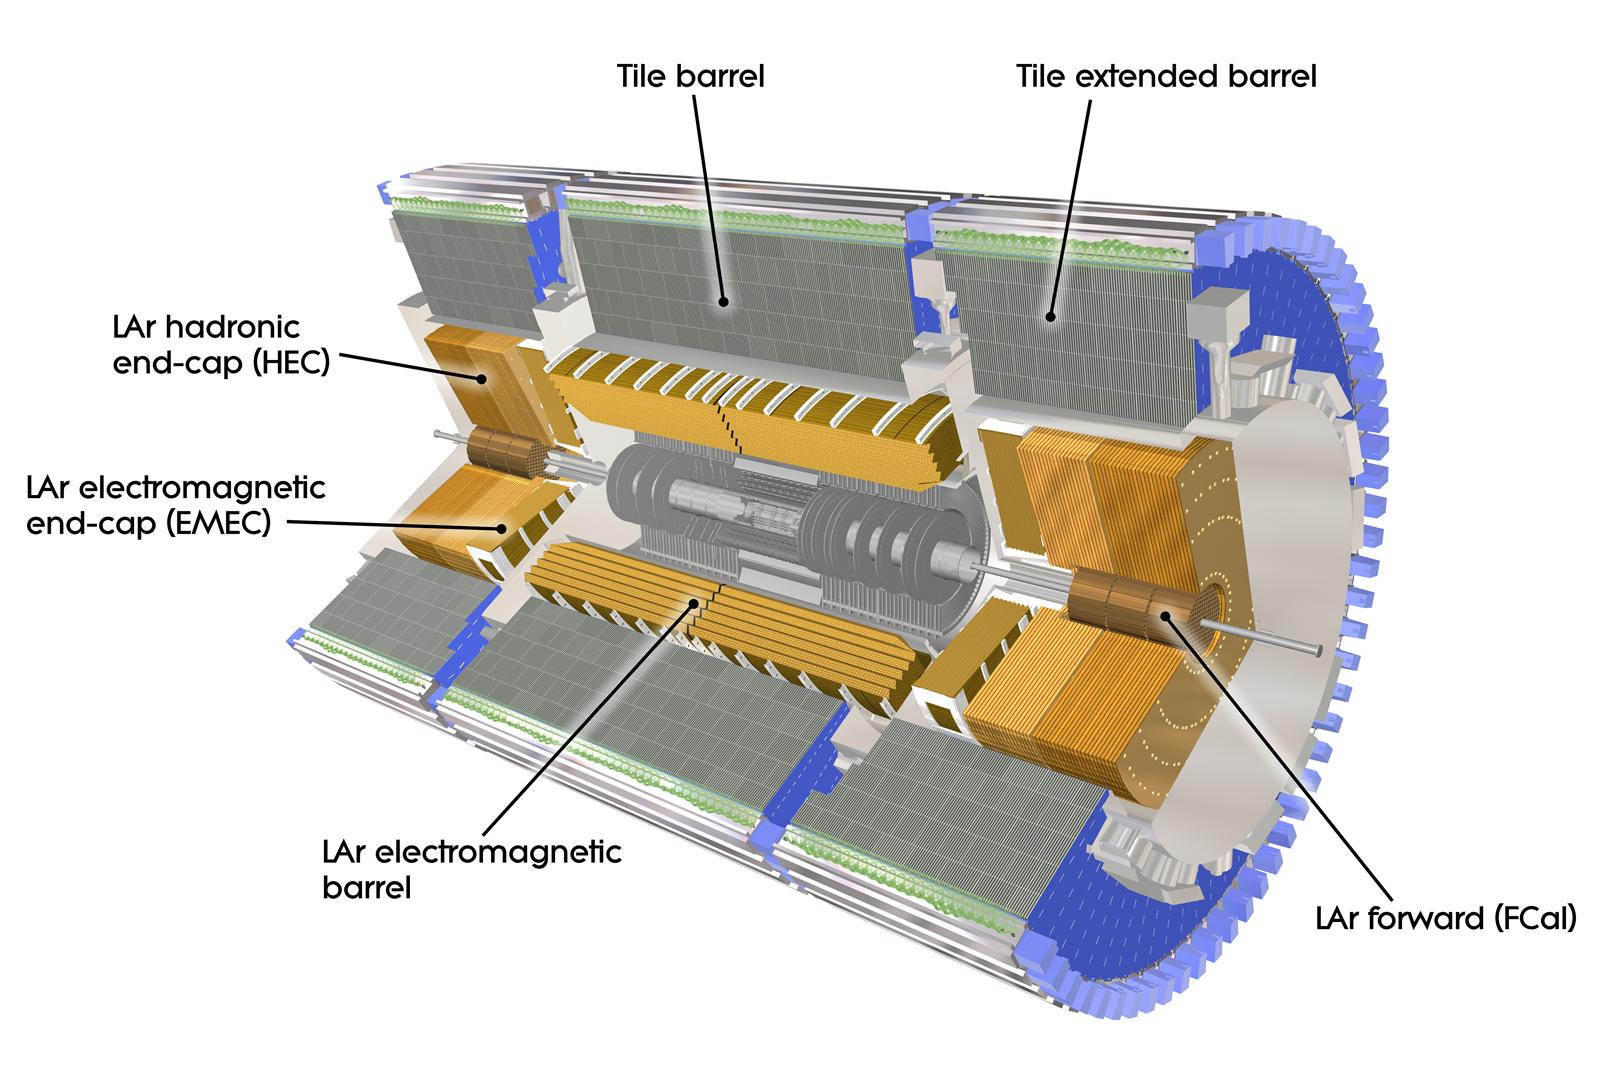
\includegraphics[width=\textwidth]{Images/ATLAS/ATLASCalo.jpg}
  \caption{The calorimeter systems of ATLAS \cite{ATLASschematics}.}
  \label{fig-AtlasDecCalo}
\end{figure}

The \gls{hcal} is designed to capture the energy of hadronic showers, with \gls{lar} as active material for the endcap and forward calorimeters and scintillating plastic tiles for the barrel. As passive material, the endcaps use copper plates, the forward calorimeters use copper and tungsten, and the tile calorimeter in the barrel uses steel. The depth of the hadronic calorimeter is approximately $10 \lambda$, where $\lambda$ is the nuclear interaction length tracking the average distance before a hadron interacts with a nucleus. The calorimeters collect the majority of the energy of hadrons, with an \gls{hcal} resolution expressed as \cite{Cavallari_2011}
\begin{equation}
  \frac{\sigma_E^{\text{HCAL}}(E)}{E} = \frac{52.9\%}{\sqrt{E}} \oplus 5.7\%.
\end{equation}
This translates into a resolution of $\sim$17\% ($\sim$6\%) at energies of $\sim$10 GeV ($\sim$100 GeV).

\subsection{Muon Detection Systems}
Muons require dedicated detection systems to be efficiently and precisely reconstructed. While they leave good tracks in the \gls{id}, muons do not leave much energy in the calorimeters due to their high mass-suppressing bremsstrahlung radiations. For this reason, the outermost subdetectors of ATLAS are specially designed to be sensitive to muons. The \textit{\gls{ms}}, shown in Figure~\ref{fig-AtlasDecMuon}, is a dedicated muon tracking system that also provides an effective triggering hardware, as described later in this chapter. The muon tracker is composed of drift tubes split between the barrel region for $|\eta| < 1.2$ and the endcaps $1.2 < |\eta| < 2.7$, with cathode strip chambers in the inner layers of the endcaps. The trigger system relies on resistive plate chambers in the barrel and thin gap chambers in the endcaps. To improve momentum and charge measurements from the reconstructed tracks, powerful superconducting toroidal magnets are used to deflect muons in the \gls{ms}. The resolution on \pt\ is measured to be of $\sim 2.3$\% (2.9\%) for muons from $Z$ decays in the central (forward) region \cite{atlasMuonPTReco}.

\begin{figure}[!h]
  \centering
  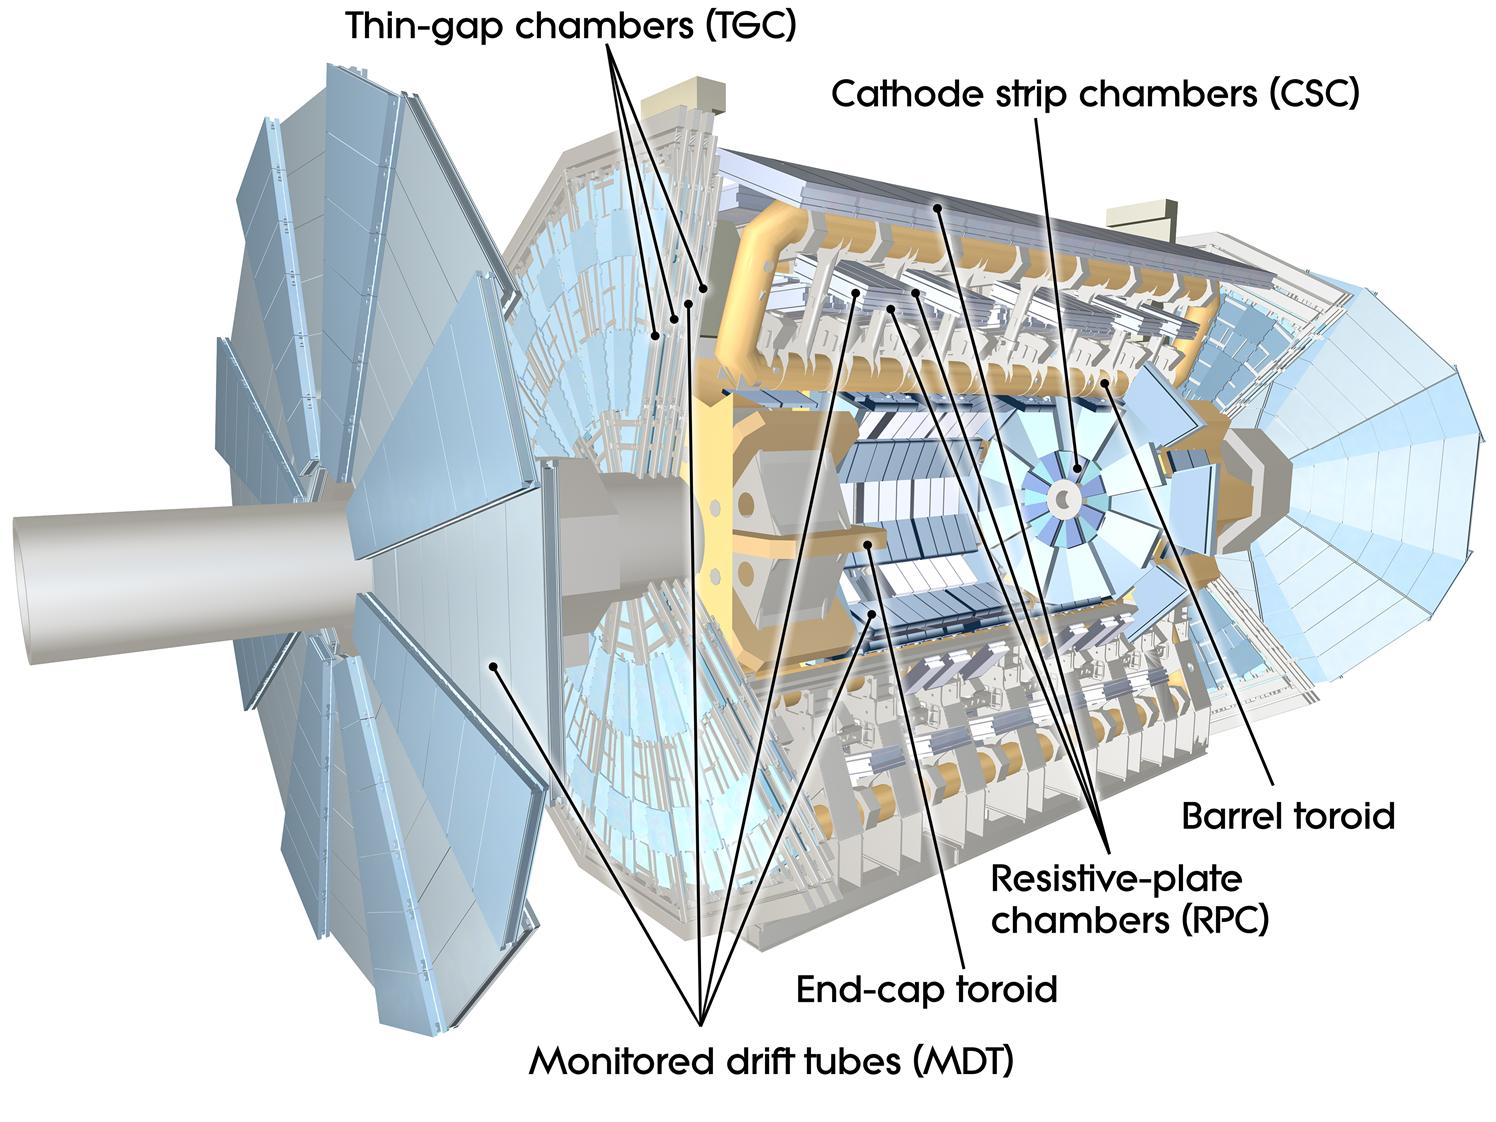
\includegraphics[width=0.9\textwidth]{Images/ATLAS/ATLASMuon.jpg}
  \caption{The muon detectors of ATLAS \cite{ATLASschematics}.}
  \label{fig-AtlasDecMuon}
\end{figure}

\section{Operation and Reconstruction with the ATLAS Detector}\label{chap-atlas-reco}
For physics-quality data taking, the different subdetectors of ATLAS must be performing according to specifications. In operation, the event rate produced by the \gls{lhc} in the heart of the ATLAS detector is 40 MHz, due to the 25 ns bunch-crossing. This unfortunately leads to a data generation rate that is too high for the computing resources available, requiring the Collaboration to design specific approaches to reduce the rate to a manageable level \cite{Nedden_2017}. This is the task of the trigger system, which is described in this section. Events that pass the trigger thresholds are stored and must be further analysed to reconstruct the physics processes from the low-level measurements performed by the different subdetectors: this is the task of reconstruction, the last subject described in this chapter for object types relevant to the presented work. This latter step is performed thanks to the extensive ATLAS software \cite{ATL-SOFT-PUB-2021-001, ATL-SOFT-PUB-2020-001}, exploiting the specific signatures of the different detected particles as schematised in Figure~\ref{fig-ATLASdetect}.

\begin{figure}[!h]
  \centering
  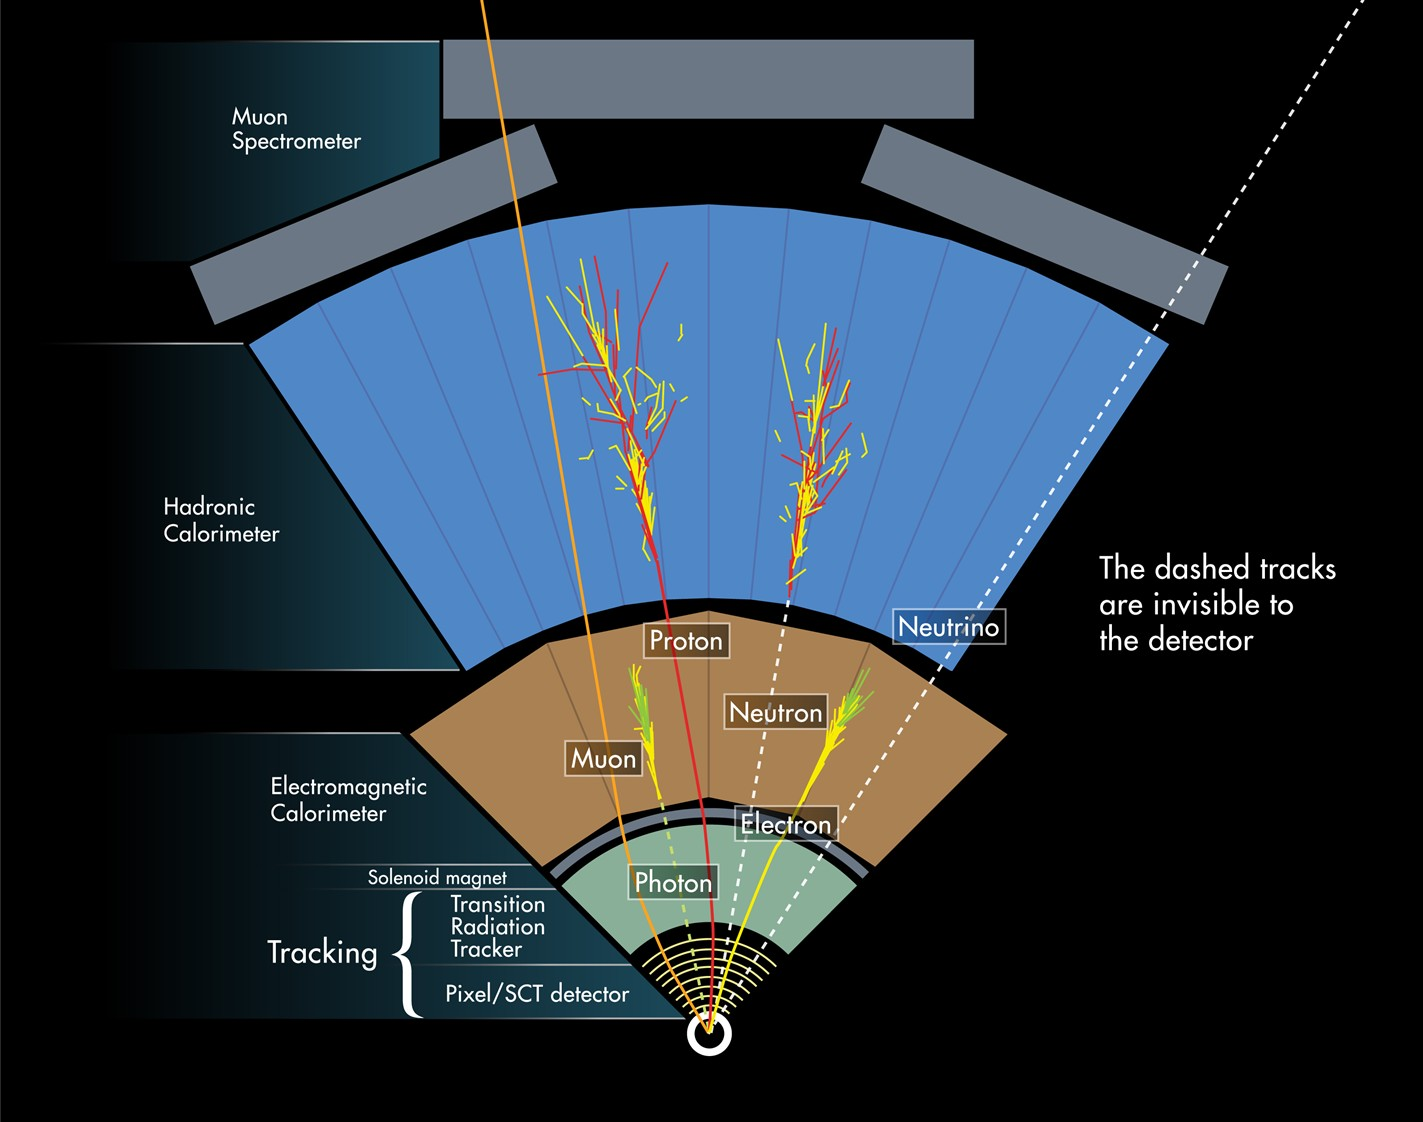
\includegraphics[width=\textwidth]{Images/ATLAS/ATLASdetection.jpg} %0.8
  \caption{Schematics of different particles signatures in the ATLAS detector \cite{Pequenao:1505342}.}
  \label{fig-ATLASdetect}
\end{figure}

\subsection{Trigger System}\label{sub-sec-trigger}
The ATLAS trigger system relies on a hierarchical approach to progressively reduce the data rate and select events deemed interesting for physics. Firstly, the Level-1 (L1) trigger is built on fast electronic hardware accessing coarse information to reduce the rate to 100 kHz in $\sim$ 2.5 $\mu$s. This is followed by the High-Level Trigger (HLT) that runs on a farm of 40,000 \glspl{cpu} to implement a finer software-based selection, bringing the rate down to 1.2 kHz or 1.2 GB/s, suitable for data storage \cite{TriggerATLAScollaboration_2020}. In this process, increasingly complex information is accessed by dedicated readout and measurement systems. Some commonly used triggers are based on signatures of electrons, muons, missing transverse energy, and $b$-jets. Different trigger menus are designed by the Collaboration, with dedicated data-taking periods for each setup. Analyses can then select data collected with the optimal trigger stream for the specific signatures sought.

\subsection{Low-Level Signatures: Tracks, Vertices, and Clusters}\label{sec-atlas-lw}
Low-level signatures are used in higher-level reconstruction processes to identify physics objects, such as electrons and jets. Three types are described here: the trajectory of charged particles called \textit{tracks}, the construction of vertices, and the formation of calorimeter clusters. \\

Tracks are the reconstructed trajectories of charged particles through the detector from the collected localised energy deposits called \textit{hits}. A \textit{hole} is a missing hit in a sensitive detector element when one is expected based on the reconstructed track trajectory. With denser pile-up activity, the number of hits in a single event becomes significant, making track reconstruction a computationally challenging problem \cite{ATL-PHYS-PUB-2015-006, ATLAS-tracks-algo,}. The trajectories are curved due to the previously described superconducting magnets. From a set of hits, tracks are fitted inside-out \cite{ATLAS-tracks-algo}: clusters of three hits in the Pixel or \gls{sct} detectors are first identified as \textit{seeds}, with additional hits associated by a combinatorial Kalman Filter \cite{10.1115/1.3662552} based on compatibility criteria with the initial track. Hits can initially be shared by several tracks, with the ambiguity resolved later when the reconstructed tracks are ranked by quality and $\chi^2$ fits are performed to quantify the best possible association while favouring high \pt\ tracks. The process is then extended to the \gls{trt} from the outside-in, and followed by additional quality criteria such as requiring tracks to have a \pt\ > 500 MeV in $|\eta| < 2.5$, a minimum of 7 hits in the Pixel and \gls{sct}, at most one hole, and at most two shared hits. Tracks are parameterised by the longitudinal (along $z$) and transverse (in the $x-y$ plane) \glspl{ip}, respectively $z_0$ and $d_0$, measuring the distance from the \gls{pv} to the point of closest approach of the track (the perigee). \\

If a reconstructed charged particle is produced in the hard scattering event, its trajectory leads back to a location called the \textit{\glsreset{pv}\gls{pv}} \cite{ATLAS:2016nnj}, where the $pp$ interaction occurs. If the particle is produced in a subsequent decay, the point of emission can sometimes be distinguished and is labelled \textit{\gls{sv}} \cite{Kostyukhin:685551}. Reconstructing the vertices is crucial for the physics programme of the Collaboration. The primary vertex is identified from a seed vertex first from the set of all well-reconstructed tracks \cite{ATL-PHYS-PUB-2015-026}. The vertex position is then iteratively refined by removing tracks incompatible with the reconstructed vertex and refitting until quality criteria are met. Discarded tracks are then used to identify secondary and tertiary vertices. The primary vertex is the one with the highest sum of squares of contributing track transverse momenta \pt. \\

In the ATLAS calorimeters, \textit{clusters} are identified by grouping cells with energy deposits matching specific criteria, using either the \textit{sliding window} or \textit{topocluster} algorithms \cite{Lampl:1099735}. The former generates fixed-size rectangular clusters by translating a window to maximize the transverse energy $E_T$ measured. The latter clusters neighbouring cells based on a signal-to-noise criterion. As the sliding window method is easier to calibrate, it is used in electron, photon, and hadronic-$\tau$ reconstruction. Topoclusters are robust against noise and are therefore used for jet and missing transverse energy reconstruction.

\subsection{Electrons}\label{sec-atlas-el}
Electrons leave signatures in the \gls{id} and the \gls{ecal}. In the central region $|\eta| < 2.5$, electrons are identified and reconstructed with both subdetectors. The forward region $2.5 < |\eta| < 4.9$ is only covered by the calorimeters, and the shape of the shower is used to identify electrons. Here, only centrally produced \textit{prompt} electron reconstruction is described, where \textit{non-prompt} electrons are not produced from the main physics process but through subsequent decays or interactions with the detector itself. \\

Since photons, pions, and jets can be mistaken for electrons, identification and isolation criteria must be implemented to provide high-purity electron candidates for analyses. The reconstruction relies on calorimeter clusters and track information. Tracks are matched to clusters with the expected energy loss taken into consideration. The track is extrapolated to ensure compatibility with the cluster barycentre, and the process is run again with more stringent conditions after refitting the matched tracks. A prompt electron is required to have a track matched to the \gls{pv}. The absence of precision hits or a matched track leads to considering the calorimeter clusters as a photon deposit. Photons can however be mistaken as electrons due to the photon-conversion process, where $\gamma \rightarrow e^+e^-$. Converted photons are allowed hits in the outer layers of the \gls{id}. \\

To further distinguish prompt electrons from non-prompt electrons and photons, a likelihood-based identification algorithm built on a \glsreset{mva}\gls{mva} discriminant is deployed \cite{Aaboud:2657964}. Features exploited include the number of hits in each tracker layer, the track \glspl{ip}, and some calorimeter cluster parameters. Several operating points that are progressively more selective are defined on the \gls{mva} discriminant, from \textit{Very Loose}, \textit{Loose}, \textit{Medium}, to \textit{Tight}. Prompt electron candidates are required to be isolated from other tracks and energy deposits, with specific isolation criteria that are either \gls{id}- or calorimeter-based. In the former case, the sum of tracks \pt\ in a $\Delta R$ cone around the electron is used, while the latter analyses the sum of calorimeter energy deposits in a cone around the electron cluster. As further described in Chapter~\ref{sec-unc}, the efficiencies of the electron reconstruction, including identification and isolation, are estimated by comparing the measured and simulated measurements of the $Z\rightarrow e^+e^-$ and $J/\psi\rightarrow e^+e^-$. 

\subsection{Muons}\label{sec-atlas-mu}
The \gls{ms} is the main detector to identify muons, with other subdetectors such as the \gls{id} used to reconstruct the properties of these leptons. Muons also leave some energy deposits in the calorimeters. The signatures in the different subdetectors are combined to reconstruct muon candidates. In the \gls{ms}, tracks are constructed from a fit of the successive hits in the different chambers. \textit{Combined muons} are defined by matching a track in the \gls{ms} to a track in the \gls{id}, with additional information from the calorimeters. \\

Prompt muons are separated from background-produced muons (such as in the decay of a $b$-hadron) by specific criteria targeting discrepancies in the \pt\ between the \gls{ms} and \gls{id}. Increasingly selective operating points are defined to identify muons as \textit{Loose}, \textit{Medium}, \textit{Tight}, and \textit{High-\pt}. Isolation requirements are applied similarly to the electron case, either track- or calorimeter-based, in a $\Delta R$ cone around the candidate muons. The calibration of muons is performed similarly to the electrons, on $Z\rightarrow \mu^+\mu^-$ and $J/\psi\rightarrow \mu^+\mu^-$ samples.

\subsection{Jets}\label{sec-atlas-jets}
Quarks and gluons are the most commonly produced particles in a hadron collider. As described in Chapter~\ref{chap-theory}, these particles carry colour charges and therefore undergo hadronisation when produced to neutralise their free colour. This complex phenomenological process leaves a unique signature in the detector: a spray of particles emitted within the original parton direction called a \textit{jet}. Electrically charged and neutral particles are contained within jets, with most of the energy deposited in the hadron calorimeters. These aggregated objects are constructed by applying a clustering algorithm on tracks and/or calorimeter clusters, depending on the jet definition. \\ 

The most notorious clustering method is the anti-$k_T$ algorithm, thanks to the robustness of the defined jets to collinear splitting and additional soft emissions \cite{Cacciari:2008gp}. The algorithm starts by considering high-momentum objects, after which softer objects are considered and potentially added to grow the jets or start a new jet. Two objects are considered at a specific step of the algorithm: the seed object $i$, either the highest momentum object or the jet in construction, and the currently unassigned highest transverse momentum object $j$. Two distances are evaluated when considering whether to cluster these objects
\begin{equation}
  d_{ij} = \min\left(\frac{1}{k_{Ti}^2}, \frac{1}{k_{Tj}^2} \right) \frac{\Delta R_{ij}^2}{R^2} \quad \text{and} \quad d_{iB} = \frac{1}{k_{Ti}^2}.
\end{equation}
The first distance, $d_{ij}$, combines the angular aperture $\Delta R_{ij} = \sqrt{(\eta_i - \eta_j)^2 + (\phi_i - \phi_j)^2}$ between $i$ and $j$ with the transverse momentum $k_T$ of the two objects and a fixed \textit{radius} parameter $R$. This distance defines a radius limiting the size of the jet cone. It is compared to the second distance, $d_{iB}$, assessing the size of the already formed jet $i$. If $d_{ij} < d_{iB}$, $j$ is clustered with $i$ into a larger jet $i$, otherwise $i$ is identified as a jet and removed from consideration. The algorithm proceeds after updating the distances until all constituents are assigned. Typical radii for ATLAS are $R = 0.4$ and $R=1.0$, defining respectively small-$R$ and large-$R$ jets. The former is commonly used for quark and gluon jets, while the latter is employed to identify heavy object decay, such as $W$ or Higgs bosons. \\

Jets can be constructed from tracks, calorimeter clusters, or both. In ATLAS, several types of jets are deployed. The following types are all reconstructed with the anti-$k_T$ algorithm but clustering different objects:
\begin{itemize}[leftmargin=*]
\item PFlow jets combine particle-flow objects \cite{atlasPFLOWjet} with a radius $R$ = 0.4. These objects combine tracking information from the \gls{id} with the calorimeter clusters, leading to a better energy resolution at low \pt\ and lower pile-up contamination after calibration \cite{PhysRevD.96.072002}.
\item EMTopo jets are constructed from denoised topological calorimeter clusters called \textit{topoclusters}, based on the per cell energy significance $S_{\text{cell}} = E_{\text{cell}} / \sigma_{\text{cell}}$, where $E_{\text{cell}}$ is the energy and $\sigma_{\text{cell}}$ the expected noise level in the cell \cite{atlasEMTOpo}. The topoclusters are then used with the anti-$k_T$ method with a small (0.4) or large (1.0) radius.
\item Large-$R$ jets are built from topological calorimeter clusters with a radius $R = 1.0$. These jets are trimmed to remove the contributions from soft contamination, which is mainly due to pile-up and underlying event activity, leading to an improved mass resolution \cite{ATLAS:largeRjet}.
\item Track-jets or \glsreset{vr} jets are constructed with a variable radius depending on the jet \pt, such that the wide cone used at low \pt\ ($R \sim 0.4$) becomes narrower at high \pt\ ($R \sim 0.02$). They are typically identified as sub-jets of a large-$R$ jet, to give access to the single-jet flavour tagging techniques described in Chapter~\ref{chap-ftag}.
\end{itemize}
PFlow and \gls{vr} jets are used to train the algorithms of Chapter~\ref{chap-ftag}, while EMTopo, large-$R$, and track-jets are used in the analysis of Chapter~\ref{chap-VH}. Jets are assigned a flavour based on the presence of an original parton within a $\Delta R = 0.3$ cone around the jet axis. Experimentally, the flavour is often determined based on the hadrons found within the jet, as described in detail in Chapter~\ref{chap-ftag}. \\

\newpage
Jets benefit from an extensive calibration to correct their reconstructed properties such as the mass, the energy, and the jet axis. In particular, corrections to account for \gls{pu} activity and out-of-cone emissions and deposits are considered. Detector effects are also taken into account, such as differences between the electromagnetic and hadronic calorimeters and leakage out of the active regions. The \textit{\gls{jes}} calibration implements these corrections in successive steps \cite{ATLASjesjerMeas}: 
\begin{itemize}[leftmargin=*]
\item \textit{Origin}: the jet axis, initially constructed from the centre of ATLAS, is corrected to point from the \gls{pv}, and the reconstructed \pt\ is updated.
\item \textit{Pile-up}: both in-time and out-of-time pile-up leave additional energy deposits in the calorimeters. This is subtracted from the jet, first from an overall estimation based on the average \gls{pu} and then from the actual number of interactions and vertices in the event. 
\item \textit{Absolute}: absolute energy corrections dependent on the energy $E$ and $\eta$ are derived to match the data energy scale to the particle-level energy scale with dedicated simulation samples.
\item \textit{Eta inter-calibration}: the detector is not homogeneous and the forward region measurements ($|\eta|>1.4$) are typically less accurate. Corrections are applied to forward jets based on central jets ($|\eta|<1.4$).
\item \textit{Global sequential calibration}: energy leakage in the calorimeters is accounted for with a set of momentum corrections based on five different observables representing the jets shape and energy.  
\item \textit{In-situ calibration}: corrects any potential differences due to an incorrect description of the detector in the simulations by performing a fit to data in the dedicated measurement of a well-reconstructed object. Events from the following processes are used at increasing \pt\ scales: $Z+$jet events with the leptonic $Z$ decays, $\gamma$+jet, and \gls{qcd} multi-jet events.
\end{itemize}
The \gls{jes} is parametrised by \pt, and uncertainties are derived for analyses to include in their modelling. The \textit{Jet Energy Resolution (JER)} is then defined as $\sigma_{p_T}/p_T$, and also calibrated with uncertainties derived from a fit to di-jet events \cite{ATLASjesjerMeas}. Despite the \gls{jes} correction procedure, \gls{pu} jets can still be significant and a \textit{\gls{jvt}} is used to reject this background \cite{ATLAS-CONF-2014-018}. This implements a 2D likelihood method built from track variables. From this discriminant, different selection criteria are derived as operating points with specific \gls{pu} jet rejections. 

\subsection{Taus}\label{sec-atlas-tau}
Taus are the heaviest generation of charged lepton, with a mass of 1.8 GeV slightly higher than that of $c$-quarks \cite{Tanabashi:2018oca}. Their lifetime is so short that they mostly decay within the beampipe. They leptonically decay 35\% of the time to neutrinos and an $e$ or a $\mu$, hence their hadronic decays are more frequent. The leptonic decays are hard to disentangle from prompt electrons and muons. Hadronic decays however leave a discernible signature reconstructed as a small-$R$ jet identified by a \glsreset{rnn}\gls{rnn}, to disentangle them from \gls{pu} and \gls{qcd} jets \cite{ATL-PHYS-PUB-2019-033}. Different operating points are derived at specific efficiencies. 

\newpage
\subsection{Missing Transverse Energy}\label{sec-atlas-met}
Some physics objects do not leave a signature in the detector, such as neutrinos. Their presence is not directly detectable but can be inferred thanks to the negligible initial \pt\ of the two interacting partons. Requiring the transverse energy \etm\ and momentum to be balanced, the missing transverse energy is calculated as the negative vectorial sum of the transverse momenta of objects, as
\begin{equation}
  \boldsymbol{E}_T^{\text{miss}} = - \sum_{\text{hard}} \boldsymbol{p}_T - \sum_{\text{soft}} \boldsymbol{p}_T,
\end{equation}
where the sum is decomposed into a \textit{hard} term encompassing all high-level physics objects and a soft term including good-quality \gls{id} tracks associated with the primary vertex but not matched to a high-level physics object \cite{ATLASmetReco}. The performance of the reconstruction is measured by comparing simulations to data, with scale and resolution derived with uncertainties to be used by physics analyses. 

\newpage
%\chapter{\color{oxfordblue} Machine Learning \& Deep Learning}
\ChapFrame

\textit{
This chapter is dedicated to a review of relevant machine learning and deep learning methods in the context of High Energy Physics (HEP). As for other fields of science and technology, the recent advancements in artificial intelligence have introduced many useful techniques that can be leveraged in particle physics. Before starting the review, some definitions of the different terms are presented. This is followed by introducing the most commonly deployed approaches in particle physics: decision trees and deep neural networks. A final word on optimisation techniques is given at the conclusion of this chapter.
}

\section{Definitions}
\subsection{Artificial Intelligence}
Artificial Intelligence encapsulates any piece of software, any \textit{program}, that aims to mimic an aspect of human intelligence, a non-exhaustive list of which includes: 
\begin{itemize}
    \item \textit{Reasoning}, the ability to conduct logical thoughts and estabish their validity.
    \item \textit{Inferring}, the ability to connect logical statements to induce or deduce new statements.
    \item \textit{Creativity}, the ability to generate new information. 
    \item \textit{Acting}, the ability to perform a task or to change the environment.
\end{itemize}
\gls{ai} research is a large field of investigation that studies these various aspects in many subjects such as robotics, \gls{nlp}, computer vision, generative modelling, and reinforcement learning. Artificial intelligence can be broadly separated into three levels according to the performance of the created system: 
\begin{enumerate}
    \item \textit{Narrow Intelligence:} representing artificial intelligence capabilities on a specified problem, for which the underlying software is uniquely trained or designed. This field includes \textit{reactive \gls{ai}}, where a model is trained to output an optimal decision or prediction based on current conditions only and \textit{limited memory \gls{ai}}, where a model is able to draw knowledge from past data to build an internal understanding of the problem and take better-informed decisions later. An example of the former is the IBM chess player Deep Blue, while the latter is most famously demonstrated by OpenAI's GPT model powering its ChatGPT chat-box. 
    \item \textit{General Intelligence:} representing an artificial intelligence capable of matching human problem-solving skills in multiple environments. In particular, this hypothetical setting would let a machine learn new tasks on its own and extrapolate from its pre-acquired knowledge, a process referred to as \textit{transfer learning}. Such a model would have the ability to adopt and combine several of the traits of intelligence and to generalise its automated learning process to any situation.
    \item \textit{Super Intelligence:} describes a hypothetical type of intelligence able to exceed human abilities and exhibit independent control of thoughts. 
\end{enumerate}

Of these, currently only the first one is accessible and widely deployed, with the second one being an ambitious focus of research for state-of-the-art research laboratories. The inception of reactive \gls{ai}, the first approach attempted, can be found in the research into games in the 50s and 60s. This paradigm saw the rise of algorithms capable of searching for the optimal move in a large space of possible actions using \textit{heuristics}, human-passed knowledge on useful features of the specific environment of the game. For example, in chess one can use the point system assigning arbitrary values to each piece to help decide what action is worthwile (e.g., a queen is worth more than a simple pion). In this reactive approach, neither the rules of the game nor the decision process are learnt. The former is forced into the search logic and the latter is the outcome of the search process. Unfortunately state space exploration of many realistic problems scales asymptotically scales with the dimension of the input, quickly rendering reactive-based approaches unable to perform in a reasonable amount of time and computing power. Combined with the need for human-encoded insight into the problem, the potential of reactive \gls{ai} is restricted to specfic well-controlled settings with a high degree of human understanding and low environment complexity. Limited memory \gls{ai} revolutionised the field by removing the need for complete human control of the data interpretation and state formulation, letting instead a well-crafted mathematical model abstract and represent the information internally. It opens the door to applications that are not otherwise realistically be feasible, such as autonomous driving, speech recognition, seamless robotics, etc. For such problems, there does not exist a problem formulation that would be compatible with a reactive-based approach. The new paradigm of limited memory \gls{ai} has also been observed to outperform reactive \gls{ai} in all settings (e.g., in chess) and can be exploited in abstract scenarios where heuristics finding is impractical or intractable. For this reason, the focus of this chapter is on limited memory \gls{ai} as exemplified by machine learning. 

\subsection{Machine Learning} 
Machine Learning (\gls{ml}) underpins the field of narrow \gls{ai} with limited memory capabilities. It represents a shift of paradigm in \gls{ai}, moving away from human-declared logic-based rules written in a specific syntax, the wholemark of reactive \gls{ai} that executes statements such as \[\textrm{\textit{If x happens, do y}},\] for an input $x$ and an output $y$. In limited memory \gls{ai}, the state representation and update steps are encoded by mathematical models of both the dataspace ($\mathcal{D}$) and the learning process: \[\forall\, x \in \mathcal{D}, \textrm{ do }f(x) = \hat{y}; \textrm{ update }f(x) \textrm{ given } (x, y),\] where $\hat{y}$ is the prediction of the model. In this case, both the internal representation of the rules and the decision-making is underpinned by the trained mathematical model $f$. Essentially, two distinct steps are applied to the model underpinned by adjustable parameters: 
\begin{enumerate}
    \item \textit{Inferring:} the model has to give its prediction $\hat{y}$ on a new data point $x$: $f(x) = \hat{y}$.
    \item \textit{Learning:} the parameters of the model are updated based on a specified training or fitting procedure, depending on whether the training will be progressively exposed to the data points of a training dataset or directly exposed to entirety of the set. The objective is to align the output of the model $\hat{y}$ with the expected behaviour $y$: given the couple $(x, y)$, let $f(x) = \hat{y} \rightarrow y$ under training convergence - this means the model $f$ has to become an accurate estimator of the label $y$. Note that not every \gls{ml} model requires a declared target output $y$, a paradigm referred to as \textit{unsupervised} learning as described later in this chapter.
\end{enumerate}
The training process closely depends on the type of model being deployed. These can be broadly separated into two groups:
\begin{itemize}
    \item \textit{Classical machine learning:} covers model exploiting specific algorithms to exploit the data in a pre-defined and fixed approach. They include linear regression, decision trees (\gls{bdt} or \gls{mva}, random forest, ...), Support Vector Machine, logistic regression, kernel methods, $k$-Nearest Neighbours, ...
    \item \textit{Deep Learning} (\gls{dl}): these methods are based on a core logical module called the Artificial Neuron. This module is stacked into layers of given width, meaning a given number of neurons, and several layers of such modules are then connected along depth. Within this category, the information flow through the network defines different types of \gls{dl}.
\end{itemize}
\gls{dl} is thus very much a part of \gls{ml}, only constituting a specialised approach to building models on a core unit. Non-\gls{dl} are often referred to as \textit{classical} machine learning and still prove valuable in many application thanks to their ease of use and their ability to be deployed in context with small dataset sizes. There are many possible tasks for a \gls{ml} model: 
\begin{itemize}
    \item \textit{Classification:} the task of assigning discrete variables, also called labels, to a datapoint: e.g., labelling a jet as a $b$-jet. The general case is multiclass, with $n$ labels possible, and a particular common case is binary classification with $n = 2$.
    \item \textit{Regression:} the task of predicting continuous variables of a datapoint: e.g., the momentum of the particle is 15 GeV/$c$. 
    \item \textit{Features extraction:} given a dataset with specific internal features, reconstruct or extract new features, e.g., given a set of tracks, reconstruct the secondary vertex. A special subcase of this category is embedding datapoints into a different space. The dimension of this final space can be smaller - the case of dimensionality reduction, e.g. performing a projection to a subspace spanned by the principal eigenvetors (those of largest eigenvalues)  with the Primary Component Analysis - or larger when embedding the data into a richer space. 
    \item \textit{Generation:} output samples from a distribution matching the training dataset distribution. E.g., Given a sample of 1 million $t\bar{t}$ events, sample 10 new datapoints from the underlying statistical model. 
    \item \textit{Anomaly detection:} identify and flag rare events in an unlabelled dataset.
\end{itemize}

To perform these different tasks, models are constructed following different paradigms of \gls{ml}, divided mostly along the lines of the amount of human intervention \cite{MurphyML}:
\begin{itemize}
    \item \textit{Supervised learning:} the data used for training is endowed with the information the model must predict. In the learning step, the model is therefore optimised to make predictions that closely align with the target. Classification and regression are the most common tasks that fall under this realm.
    \item \textit{Unsupervised learning:} the data is not endowed with extra-information the model must learn to predict but rather has underlying features that must be extracted. The model is therefore trained with an objective to optimise without explicit targets, and should discover patterns and insights without any guidance. Generative models and clustering are prime examples. 
    \item \textit{Semi-supervised learning:} also called \textit{weak supervision}, is a paradigm combining the supervised and unsupervised approaches. The model is mostly unsupervised but can benefit from some labelled cases or human input (a technique also named \textit{active learning}). A prime example is a clustering unsupervised tasks followed by a classification of the formed clusters. This is particularly fruitful when the cost of labelling the data is expensive, as is the case with real human-linked data but thankfully not so in the case of particle physics data.
    \item \textit{Self-supervised learning:} a machine instructs itself on what tasks should be learnt. The overarching goal of the model is loosely defined and the learning process should include superficial objectives to learn.
    \item \textit{Reinforcement Learning:} this paradigm of \gls{ml} is dedicated to the setting of a game theoretic environment. An agent must explore and interact with its environment by choosing a specific action policy - a method by which the agent selects an action given its current situation and expected reward. In \gls{rl}, the objective is for the agent to learn how to construct the best policy to satisfy a reward function and therefore obtain the best outcome for itself.
\end{itemize}

These different settings can be explored in \gls{ml} and more spefically in deep learning. The latter is widely considered to be the most performant one thanks to its ease of scaling and is the main focus of research at the moment.

\subsection{Deep Learning} 
Deep Learning (\gls{dl}) combines a family of methods predominantly derived in the 1980s that have quickly grown in popularity around 2010, with widely advertised results on competitive benchmark tasks in pattern recognition, as exemplified by the super-human performance of the \textit{DanNet} model \cite{DanNet} based on \gls{cnn} \cite{NIPS198953c3bce6}. The basis of any \gls{dl} method is the Artificial Neuron, a logical unit built to mimic the functioning of a human neuron. Several such neurons are then combined into layers of any numbers of neurons (the width of the layer) and the layers themselves are stacked into depth, with deeper layer receiving as input the output of earlier layers. Different \gls{dl} models are constructed by modifying the structure of the layers - in particular, the input, output, and activation function used - and the transfer of information between neurons, be that between layers, depth-wise, or between neurons, width-wise. \gls{dl} is specifically well-suited to the setting of the \gls{atlas} experiment, because:
\begin{itemize}
    \item Large datasets of both real and simulated data are available.
    \item Thanks to advanced \gls{mc}-based simulation programs of both the physics process and the detector reconstruction effets, the simulated data points are faithful representations of the real data.
    \item The data and data-model from which the data originates is well understood in physics, the former coming from measurements from well-calibrated detectors and the second from crafted theories of the field. 
    \item The data exhibits reach features due to the collection of different detectors and the different scales of the underlying physicsprocesses. The typical available representations span images, sequences, sets, and graphs, all four being the main data representations studied throughout the deep learning community.
\end{itemize}
Given how important this form of \gls{ai} has become in all technological fields, this chapter is primarily dedicated to introducing some of its approaches most relevant to \gls{hep}. 

\section{Machine Learning Methods for Physics}
High-energy physicists enjoy a special relationship with \gls{ml} methods. Experimental particle physics largely relies on statistical analyses of complex and large datasets, be that simulated using \gls{mc} methods or collected from sophisticated detector apparata. A typical physics' analysis can be described as the combination of five main steps:
\begin{enumerate}
    \item Data collection: real data is collected from a detector exposed to the underlying physics desired, e.g., at \gls{cern} placing and callibrating the \gls{atlas} detector at an interaction point of the \gls{lhc} to collect proton-proton collision data. 
    \item Simulated data is generated to match the condition of collection of the real data in terms of detector effects and operational conditions such as energy, \gls{pu} and luminosity. This simulated data englobes the best of our current theorical knowledge of the law of physics. 
    \item The detector of a modern particle physics experiment is a complex set of sub-detectors sensitive to different physical phenomena, as described in chapter REF. % TODO ADD CHAPTER REF
    This low-level information collected by different devices must be processed and recombined to generate \textit{objects}, aggregated information that often hold physical meaning. For examples, from hits in the tracking detector a track can be fitted and some of its physical properties, such as \pt, reconstructed. This task corresponds to a mapping \textit{low}-level $\rightarrow$ \textit{high}-level information to reconstruct interesting and physically meaningful features of the measured data. 
    \item An analysis strategy is established, with objective to similarly restrict the full datasets of both simulated and real data to a portion of the dataspace that is most sensitive to the studied \textit{signal} or process. The sensitivity aspect underlies the need to take into account limited knowledge of theorical physics, limited precision of the apparata, limited statistics of both simulations and data collected, etc. To optimise the analysis, selection rules are derived based on physically accessible information, e.g., the centre-of-mass energy, presence of leptons, the transverse momentum \pt, and other high-level object reconstructed in the previous step.
    \item With the optimally selected set of real and simulated datapoints, a statistical model is built to quantify the agreement of the measured data with the expectations from the theory under the conditions of the experiment. This is most often achieved through a profile likelihood computation, where the parameters of interested target by the analysis are measured to be those maximising the likelihood under the given measured data.
\end{enumerate}

Modern advanced machine learning has the potential to improve all steps of this process:
\begin{enumerate}
    \item The operational side of running the detector and the accelerators can benefit from \gls{rl} methods for improved control of the different electronic device and accelerator control. Triggers, an essential component of the \gls{atlas} experiment described later in this thesis, can be upgraded to use sophisticated \gls{dl} model running online thanks to a hardware back-bone built on \gls{fpga} or \gls{gpu}.
    \item Simulating a dataset using a \gls{mc} approach is a computationally intensive task. Each event must pass through a selection of probabilistic step, with only a simulated datapoint sastifying all requirements ending in the usable sample. This process can be sped-up and optimised significantly with more advanced and refined \gls{mc} methods, but the cost remains significant to generate datasets of sufficient statistics. Generative \gls{ai} has the potential to accelerate this step by giving statistical model that can be efficiently sampled. \gls{gan} and \gls{vae} have been shown to perform the sampling step in a competitive amount of time. However, a key limitation of these stasticial approach is their limited ability to encorporate the sophisticated theorical model required to simulate the data, and any discrepancy or unclosure introduces levels of disagreements that are counter-productive to the final objective of the physics analysis.
    \item \gls{ml} is particularly well-suited for the object reconstruction task. Broadly, \gls{ml}-based method can offer scalable, efficient, and precise solutions for objects reconstruction. Important examples in \gls{atlas} are identifying particles in the detector (e.g., $\tau$ identification), reconstructing missing transverse energe ($E_T$), and classifying heavy-flavour jets - as exemplified in the next chapter of this thesis dedicated to flavour tagging. % TODO check its the right chapter and refer to it
    \item Historically, physicists have relied on a cut-base approach to select their data: they analyse each of the relevant variables for the physics problem at hand to try and identify the best features to use to restrict the dataspace through manually-defined restrictions. For example, to a measure an interesting physical quantity of the process of $Z$-bosons decaying to two charged leptons $l^+l^-$, restricting the invariant mass of the lepton pair $m_{l^+l^-}$ to lie close the $Z$-boson rest mass $m_Z \approx 91.19$ GeV/$c^2$ is beneficial, as most of the signal will be found there. Machine learning is able to entirely bypass this manual operation, learning directly from an appropriate set of signal and background datasets with given features a transformation of the input data features to a discriminant optimising the separation of signal from background. 
    \item The likelihood function of the constructed statistical test, verifying the level of agreement between the real data and the theory through the simulated sample, can be directly learnt by a model given access to both sets. Furthermore, anamoly detection settings, such as those in the search for unknown resonances, can be derived using \gls{ml} model in an unsupervised setting, thereby automating the discovery process and requiring only real data. 
\end{enumerate}

One of the main focus of this thesis can be broadly summarised as contributing to step 3 in the aformentioned list: developping \gls{dl}-tools for improved object reconstruction. The analysis presented in the latter part of this document also introduces some classical \gls{ml} technique of data selection - corresponding to step 4. The rest of this chapter now address a more detailed review of the relevant \gls{ml} methods. 

\subsection{Decision Trees}
\gls{dt}, also called \textit{Classification and Regression Trees} (CART) are the bread-and-butter of any data analysis. They are simple to train, give a good ground performance for both classification and regression tasks, and are white box model - meaning there decision process is easy to interpret. Underlying the model is a recursive partitioning approach of the input space \cite{MurphyML}. Labelling a partition step as \textit{node}, the tree structure emmerges from a \textit{root} state that is subsquently partitioned along different branches with one \textit{leaf} per final region. The splits are done along a feature of the input space, and the method accept both discrete categorical values (e.g., the label of a lepton as $e, \mu, \tau$) and continuous values (e.g., $m_l$). For example, the following is a simple classification tree outputting the predicted class as 0 or 1:

\Tree[.\textit{$x_i \leq c_i$} [.{True \\\textit{$x_j \geq c_j$}} [.True 1 ]
            [.False 0 ]]
        [.{False \\\textit{$x_k \leq c_k$}} [.True 0 ]
            [.{False \\{\textit{$x_l$} is \textit{$e$}}} [.True 0 ]
                            [.False 1 ]]]]

At each node there is a learnt condition with $x_i, x_j, x_k$ being continuous features of the dataset that are cut at the thresholds $c_i, c_j, c_k$ and $c_l$ is a categorical feature (e.g., is the lepton an electron). The leaf values are the output of the tree in different regions defined by the combination of successive selections - here a binary variable indicating a class. An example of a tree performing classification is shown in Figure \ref{fig:tree-ex}, where a tree with two nodes is able to isolate most of the blue class from the red class with the region limited by green lines, corresponding to both conditions $x_1 \geq c_2$ and $x_2 \geq c_2$ being satisfied.

\begin{figure}[h!]
    \center
    \begin{minipage}[c]{0.3\textwidth}
        \caption{A binary classification problem with two features. A decision tree applies two successive cuts $c_1$ and $c_2$ to isolate most of the blue class from the red.}\label{fig:tree-ex}
      \end{minipage}
      \begin{minipage}[c]{0.5\textwidth}
        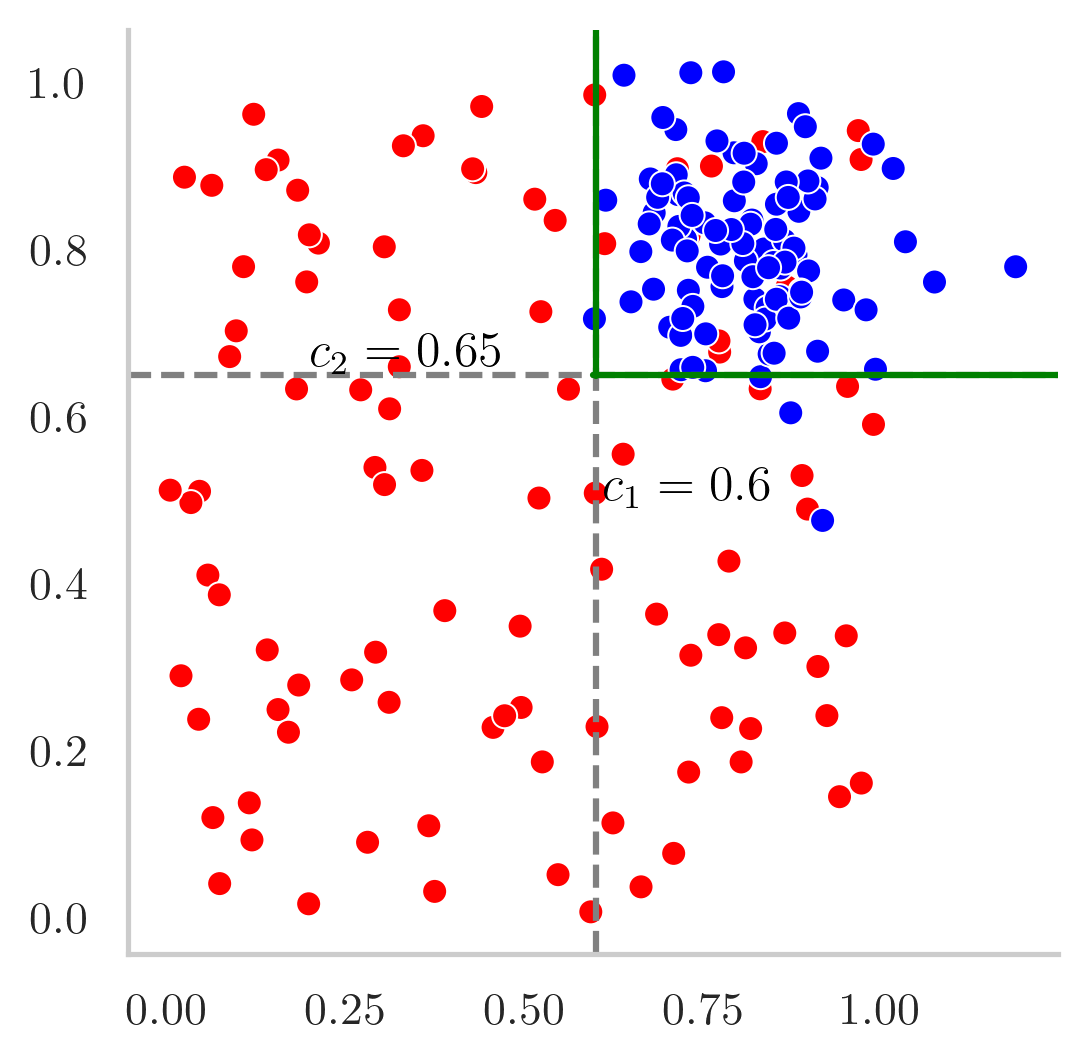
\includegraphics[width=\textwidth]{Images/ML/scatterPlot.png}
      \end{minipage}
\end{figure}
    
Finding the optimal set of partitions of a dataset is an NP-complete problem and therefore intractable for large datasets. To build a tree, a greedy approach must be adopted - meaning using a heuristic approach to find a satsifying solutions, e.g., successively choosing the most optimal step at each stage with no guarantee to find a global optimum instead of a local one. The chosen split is selected based on a defined \textit{cost} function as suggested in Equation \ref{eq:DTcost}.

\begin{equation}\label{eq:DTcost}
    (j^*, t^*) = \arg\min_{j\in \{1, ..., D\},\, t \in T_j} \min \left(\text{cost} (\{x_i, y_i : x_{ij} \leq t\}) + \text{cost}(\{x_i, y_i : x_j > t\}) \right)
\end{equation}
where $T_j$ is the set of possible thresholds, $x_j$, $y_j$ are the features and label (or regressive objective). For categorical variable, the inequality $x_j >< t$ is converted in a value equality $x_j == t$. The \textit{cost} function will depend on the objective of the tree, with the regression case typically using the error function \[cost(D) : \sum_{i\in D}(y_i - \bar{y})^2,\] and for a classification the loss would be one of the following:
\begin{itemize}
    \item \textit{Missclassification rate:} $\frac{1}{|D|} \sum_{i \in D} \mathbb{I}(y_i \neq \hat{y})$, where $D$ is the data in the leaf of the tree and $\mathbb{I}$ is the identity function: $\mathbb{I}(x) = 1$ if $x$ is True, else $0$. 
    \item \textit{Statistical entropy:} defining the class-condition probability as $\pi_c = \frac{1}{|D|} \sum_{i \in D} \mathbb{I}((y_i) \neq c)$, the entropy over the ($C$) classes is defined in Equation \ref{eq:statEntropy}
    \begin{equation}\label{eq:statEntropy}
        H(\vec{\pi}) = - \sum_{c=1}^C \pi_c \log \pi_c,
    \end{equation}
    with $\vec{\pi}$ being a vector ($\pi_1, \pi_2, ..., \pi_C$) with the class-condition probabilities as components.
    \item \textit{Information Gain:} an equivalent formulation to the entropy, where the gain in information that should be maximised is the relative change in entropy by adding a selection on feature $X_j$ over the current stage: 
    \[ \text{Gain}(X_j < t, Y) = H(Y) - H(Y | X_j < t) \]
    \item \textbf{Gini:} computes and minimises the expected error rate:
    \begin{equation}\label{eq:giniClass} 
        \sum_{c=1}^C \pi_c (1 - \pi_c).
    \end{equation}
\end{itemize}

The pseudocode algorithm to train a \gls{dt} with the update rule of Equation \ref{eq:DTcost} is summarised in Algorithm \ref{ag:DT}. 

\begin{algorithm}
    \caption{Recursive Procedure to Train a Decision Tree \cite{MurphyML}.}
    \begin{algorithmic}
    \Function{fitTree}{node, $D$, depth}
        \State $\text{node.prediction} \gets \text{mean}(\{y_i : i \in $D$\})$ 
        \State $(j^*, t^*, D_L, D_R) \gets \text{split}(D)$
        \If{\text{not worthSplitting}(\text{depth}, \text{cost}, $D_L$, $D_R$)}
            \State \Return node
        \Else
            \State node.left $\gets$ FITTREE(node, $D_L$, depth + 1)
            \State node.right $\gets$ FITTREE(node, $D_R$, depth + 1)
            \State \Return node
        \EndIf
    \EndFunction
    \end{algorithmic}
    \label{ag:DT}
\end{algorithm}

\gls{dt} can overfit a dataset: the model may tune itself to specific features of the training set that are not generalisable to any set samples from the true original distribution. Regularisation serves as an important step to avoid this often undesirable behaviour. For trees, a natural procedure to avoid overtraining is to interrupt the growth of the tree when it is no longer worth doing so - a criterion that is hard to decide \textit{a priori} - or to \textit{prune} the tree - removing nodes or branches that contribute little to the overall performance. A simpler way to regularise the performance by reducing the variance of the estimate of the model is to train several trees with different subsets of the data chosen randomly with replacement and aggregate the results into a single prediction. For example, for regression, one can take as output the average over each base learners: \[ y(x) = \frac{1}{N_l} \sum_{i=1}^{N_l} y_i(x),\] for $N_l$ base learner making prediction $y_i(x)$ given the input features $x$ and for classification select the class by majority voting. This statistical technique of using ensemble of predictors is referred to as \textit{bagging}. To further decorrelate the performance of the different predictors, these can be built on a subset of the input features and training datapoints, thereby forming a \textit{random forest}.

\subsection{Boosted Decision Trees}
A popular extension to the simple decision trees approach is to introduce the concept of \textit{boosting}, leading to a model referred to as a Boosted Decision Trees (\gls{bdt}) or \gls{mva} in particle physics. Boosting is a greedy algorithm leveraging a weak learner or predictor (e.g., a \gls{dt}) and applying it sequentially to weighted versions of the data, with a larger weight given to missclassified or miss-regressed datapoints, as per the use case. This method is hugely popular in data science, having earned the title \textit{``best off-the-shelf classifier in the world''} \cite{baggingML}. Two particularly useful approaches are adaptive boosting (AdaBoost) \cite{Adaboost} and gradient boosting \cite{gradientBoosting}, both combining an ensemble of $M$ weak learners $f_i$ ($i = 1, ..., M$) into a strong learner $F$: \[F(x) = \sum_{i=1}^M f_i(x).\] For the following discussion, the model is built using a training dataset $ \{(x_1, y_1), ..., (x_N, y_N)\}$ with input vectors $x_i \in \{\mathbb{R} \otimes \mathbb{D}\}^d$ of $d$ features that are real or discrete ($\mathbb{D}$) and $y \in \mathbb{R}^d$ is a $d$-dimension real vector that serves as output to be predicted by the model.

\subsubsection{AdaBoost}
AdaBoost combines the $M$ weak learners $f_i$ with adaptive weights $\alpha_i$ to improve the ensemble performance as \[F(x) = \sum_{i=1}^M \alpha_i f_i(x),\] where $F$ is the boosted model, and the successive boosting stages $F_T = \sum_{i=1}^{T \leq M} \alpha_i f_i(x)$ define stronger and stronger boosted variants of the model that combine weak learners $f_i$ with a weight $\alpha_i \in \mathbb{R}$. At each iteration $m$ of the training process ($m = 1, ..., M$), a weak learner $f_m$ is fitted to the training set to minimise a loss function $L(y_i, F_{m}(x_i))$. The loss in AdaBoost is the exponential loss on the datapoints of Equation \ref{eq:adaboosterror}:

\begin{equation}\label{eq:adaboosterror}
    L(y, F_m(x)) = \sum_{i=1}^N \exp\left(-y_i F_m(x_i)\right) = \sum_{i=1}^N \exp\left(-y_i (F_{m-1}(x_i) + \alpha_m f_m(x_i))\right),
\end{equation}
that the added new weak learner $\alpha_m f_m$ at step $m$ has to minimise: $(\alpha_m, f_m) = \arg \min_{(\alpha_m, f_m)} L(y, F_m(x))$. The typical case for AdaBoost is binary classification with $y_i \in \{-1, 1\}$ but the algorithm can be generalised to other cases \cite{MurphyML}. Equation \ref{eq:adaboosterror} can be re-expressed as: \[\sum_{i=1}^N w_{i,m} \exp\left(-\alpha_m y_i f_m(x_i)\right),\] where $w_{i,m} = \exp\left(-y_i F_{m-1}(x_i)\right)$ can be interpreted as a weight applied to the datapoint indexed by $i$ $(x_i, y_i)$ at step $m$ proportionaly to the error of the current strong learner. It can be shown that the weak learner $f_m$ minimising the optimisation objective at step $m$ is the one minimising the miss-classified weights sum error $\epsilon_m$ of the reweighted version of the dataset with weights $w_{i,m}$ \cite{MurphyML}, where: \[\epsilon_m = \sum_i w_{i,m} \mathbb{I}(y_i \neq f_m(x_i)).\] For the first time step $m = 1$, these weights are initialised to $1 / N$. The weights are then updated to \[w_{i,m+1} = w_{i,m} e^{-\alpha_m y_i f_m(x_i)},\] and renormalised so that $\sum_i w_{i, m+1} = 1$ before being assigned to each training sample $i$ for the next step. The weak learner can be combined with the strong learner using an optimal weight $\alpha_m$ found by minimising the loss $L$ of the combined learner: \[\alpha_m = \frac{1}{2} \log \frac{1 - \epsilon_m}{\epsilon_m},\] giving the overall update rule of Equation \ref{eq:updateOverall}:
\begin{equation}\label{eq:updateOverall}
    F_m(x) = F_{m-1}(x) + \alpha_m f_m(x),
\end{equation}
combining the new weak learners $f_m$ with optimal weight $\alpha_m$ to the current strong learner. The AdaBoost algorithm is summarised in Algorithm \ref{algo:adaboost}.

\begin{algorithm}
    \caption{Adaboost for Binary Classification with Exponential Loss \cite{MurphyML}}
    \label{algo:adaboost}
    \begin{algorithmic}
    \State Initialise weights: $w_{i,1} = \frac{1}{N}$, where $N$ is the number of samples.
    \For{$m = 1$ to $M$}
        \State Minimise $\epsilon_m = \sum_i w_{i,m} \mathbb{I}(y_i \neq f_m(x_i))$ on training set with weights $w_{i,m}$ to find $f_m(x)$.
        \State Compute $\alpha_m = \frac{1}{2} \log\left(\frac{1 - \epsilon_m}{\epsilon_m}\right)$.
        \State Update weights: $w_{i,m+1} \leftarrow w_{i,m} \, \exp(-\alpha_m y_i f_m(x_i))$ and renormalised $\sum_i w_{i, m+1} = 1$.
    \EndFor
    \State \Return $F(x) = \sum_{m=1}^M \alpha_m f_m(x)$
    \end{algorithmic}
\end{algorithm}

\subsubsection{Gradient boosting}
Gradient boosting is a generic approach which, contrary to AdaBoost, does not require a specific derivation for each loss function. The objective is to minimise the empirical risk, the expected value of the loss function $L$ on the training set as shown in Equation \ref{eq:empRisk} 
\begin{equation}\label{eq:empRisk}
    \hat{f}  = \arg \min_f \mathbb{E}_{x,y} L(y, f(x))
\end{equation}
where $f(x) = (f(x_1), ..., f(x_N))$ is the output of the learner on the whole training set. As the name suggests, the approach leverages gradient descent to find the optimal $\hat{f}$. At step $m$, the gradient of the loss $L$ is evaluated at $f = f_{m-1}$ as \[ g_{i,m} = \left[ \frac{\partial  L(y_i, f(x_i))}{\partial f(x_i)} \right]_{f= f_{m-1}}, \] which is then used to update the learner with a step \[ f_m = f_{m-1} - \alpha_m g_{m},\] where $g_m$ = ($g_{1, m}, g_{2, m}, ..., g_{N,m}$) and the step-length $\alpha_m$ is chosen to minimise the residual loss $L(y, f_{m-1}$ $- \alpha_m g_{m})$. This implements functional gradient descent, and leads the model to fit the $N$ datapoints of the set. This procedure naturally leads to overfitting the training set, an undesirable feature that is remedied by using a weak learner to approximates the negative gradient. In the specific case of gradient boosted decision trees, at step $m$ a decision tree $h_m(x)$ is fitted to the pseudo-residuals $g_{i,m}$. This \gls{dt} $h_m$ at step $m$ defines $J_m$ disjoint regions through its leaves with predictions $b_{jm}$ in each $j = 1, ... J_m$ region: \[ h_m(x) = \sum_{j=1}^{J_m} b_{jm} \textbf{1}_{R_{jm}}(x),\] where $\textbf{1}_{R_{jm}}(x)$ is the indicator function - equals to 1 when $x \in R_{jm}$ and 0 otherwise. The update to the model is chosen so that: \[f_m(x) = f_{m-1} + \alpha_m h_m(x),\] with $\alpha_m$ selected by minimising the empirical risk of the updated model: \[ \alpha_m = \arg \min_{\alpha} \sum_{i=1}^N L(y_i, f_{m-1}(x_i) + \alpha h_m(x_i)).\]

\begin{algorithm}
    \caption{Gradient Boosting \cite{MurphyML}}
    \label{algo:gradient_boosting}
    \begin{algorithmic}
    \State Initialise $f_0(x) = \arg\min_\alpha \,\sum_{i=1}^N L(y_i, \alpha)$
    \For{$m = 1$ to $M$}
        \State Compute the gradient residual for each $i= 1, ..., N$: $g_{i,m} = -\left[\frac{\partial L(y_i, f(x_i))}{\partial f(x_i)}\right]_{f(x_i) = f_{m-1}(x_i)}$
        \State Train weak learner $h_m$ on the dataset $\{(x_i, g_{i,m})\}_{i=1}^N$
        \State Compute $\alpha_m$ by minimising $\sum_{i=1}^N L(y_i, f_{m-1}(x_i) + \alpha h_m(x_i))$
        \State Update $f_m(x) = f_{m-1}(x) + \nu \alpha_m h_m(x)$
    \EndFor
    \State \Return $f(x) = f_M(x)$
    \end{algorithmic}
\end{algorithm}

The full algorithm for Gradient Boosting is presented in Algorithm \ref{algo:gradient_boosting}, where the update rule is added a \textit{learning rate} hyperparameter $\nu$ to introduce regularisation and reduce the risk of overfitting. By keeping $0 < \nu \leq 1$, it limits the ability of the model to fully adapt to the training error, thereby improving generalisation. The price is a slower updating of the model and therefore a more demanding computational complexity. Further regularising techniques are bootstrap aggregation - training each weak learner on a random subset of the data -, limiting the number of leaves, or more generally penalising model of larger complexity - removing branches that do not reduce the loss by a minimal amount. \\

\gls{bdt} resist better to overtraining thanks to the regularisation effect of boosting and the different techniques described in this section. Unfortuntaly, an undiserable feature of boosting is the loss of direct interpretability of the decision-making but this is more than met by an appreciable \textit{boost} in performance of the underlying model. An interesting property exhibited by all tree-based algorithms and many \gls{ml} approaches is the ease to quantify the impact of a specific feature on the result. This technique of \textit{feature importance} assigns a score to each input feature, typically the Gini importance of Equation \ref{eq:giniClass}, quantifying the reduction in entropy obtained by adding a feature, or the Shapley value, measuring the average marginal contribution of each feature.  

\paragraph{Pros:}
\begin{itemize}
    \item \textit{Adaptability to Different Distributions:} Boosting algorithms, such as AdaBoost and Gradient Boosting, can adapt well to different types of data distributions and can capture non-linear relationships in the data.
    \item \textit{High Accuracy:} \gls{bdt} easily achieve high accuracy in both classification and regression tasks, making them suitable for a wide range of applications.
    \item \textit{Ensemble Learning:} The boosting technique leverages ensembling by combining multiple weak learners to create a strong learner, improving overall model performance.
    \item \textit{Robustness to Overfitting:} Boosting helps mitigate overfitting, enhancing the  generalisation of the model to unseen data. \gls{bdt} typically perform reasonably well out-of-the-box. 
    \item \textit{Feature Importance:} \gls{bdt} provide a measure of feature importance, aiding in feature selection and interpretability of the model.
\end{itemize}

\paragraph{Cons:}
\begin{itemize}
    \item \textit{Sensitivity to Noisy Data:} \gls{bdt} can be sensitive to noisy data and outliers, potentially leading to overfitting.
    \item \textit{Computational Complexity:} Training multiple weak learners sequentially can be computationally expensive, especially for large datasets or deep tree structures.
    \item \textit{Parameter Tuning:} \gls{bdt} still require some fine-tuning of the hyperparameters, such as learning rate and tree depth, for optimal performance.
    \item \textit{Black Box Nature:} The ensemble nature of boosted decision trees make them somewhat of a black box, sacrifing the perfect interpretability of \gls{dt} for the sake of performance.
\end{itemize}

\subsection{Artificial Neurons}
The Artificial Neuron, also called the \textit{perceptron} by its inventor Frank Rosenblatt in his seminal 1958 paper \cite{rosenblatt1958perceptron}, is the logical gate that underpins most \gls{dl} models. Notably, a \gls{mlp} - also called a \gls{dnn} - is a stacking of layers of artificial neurons. Inspired by biological principles, the perceptron, as shown in Figure \ref{fig:annModel}, accepts multiple intputs and gives as output 1 if the combination of inputs exceeds a certain modifiable threshold, otherwise giving 0. This combination accepts weights to scale the input which, remarkably, can be adjusted during a training phase if the output of the perceptron is incorrect. Artificial neurons are a direct generalisation of this very principle, with the output no longer being thresholded but applied a chosen function $f$ after being added a learnable bias term $b$. 

\begin{figure}[h!]
    \center
    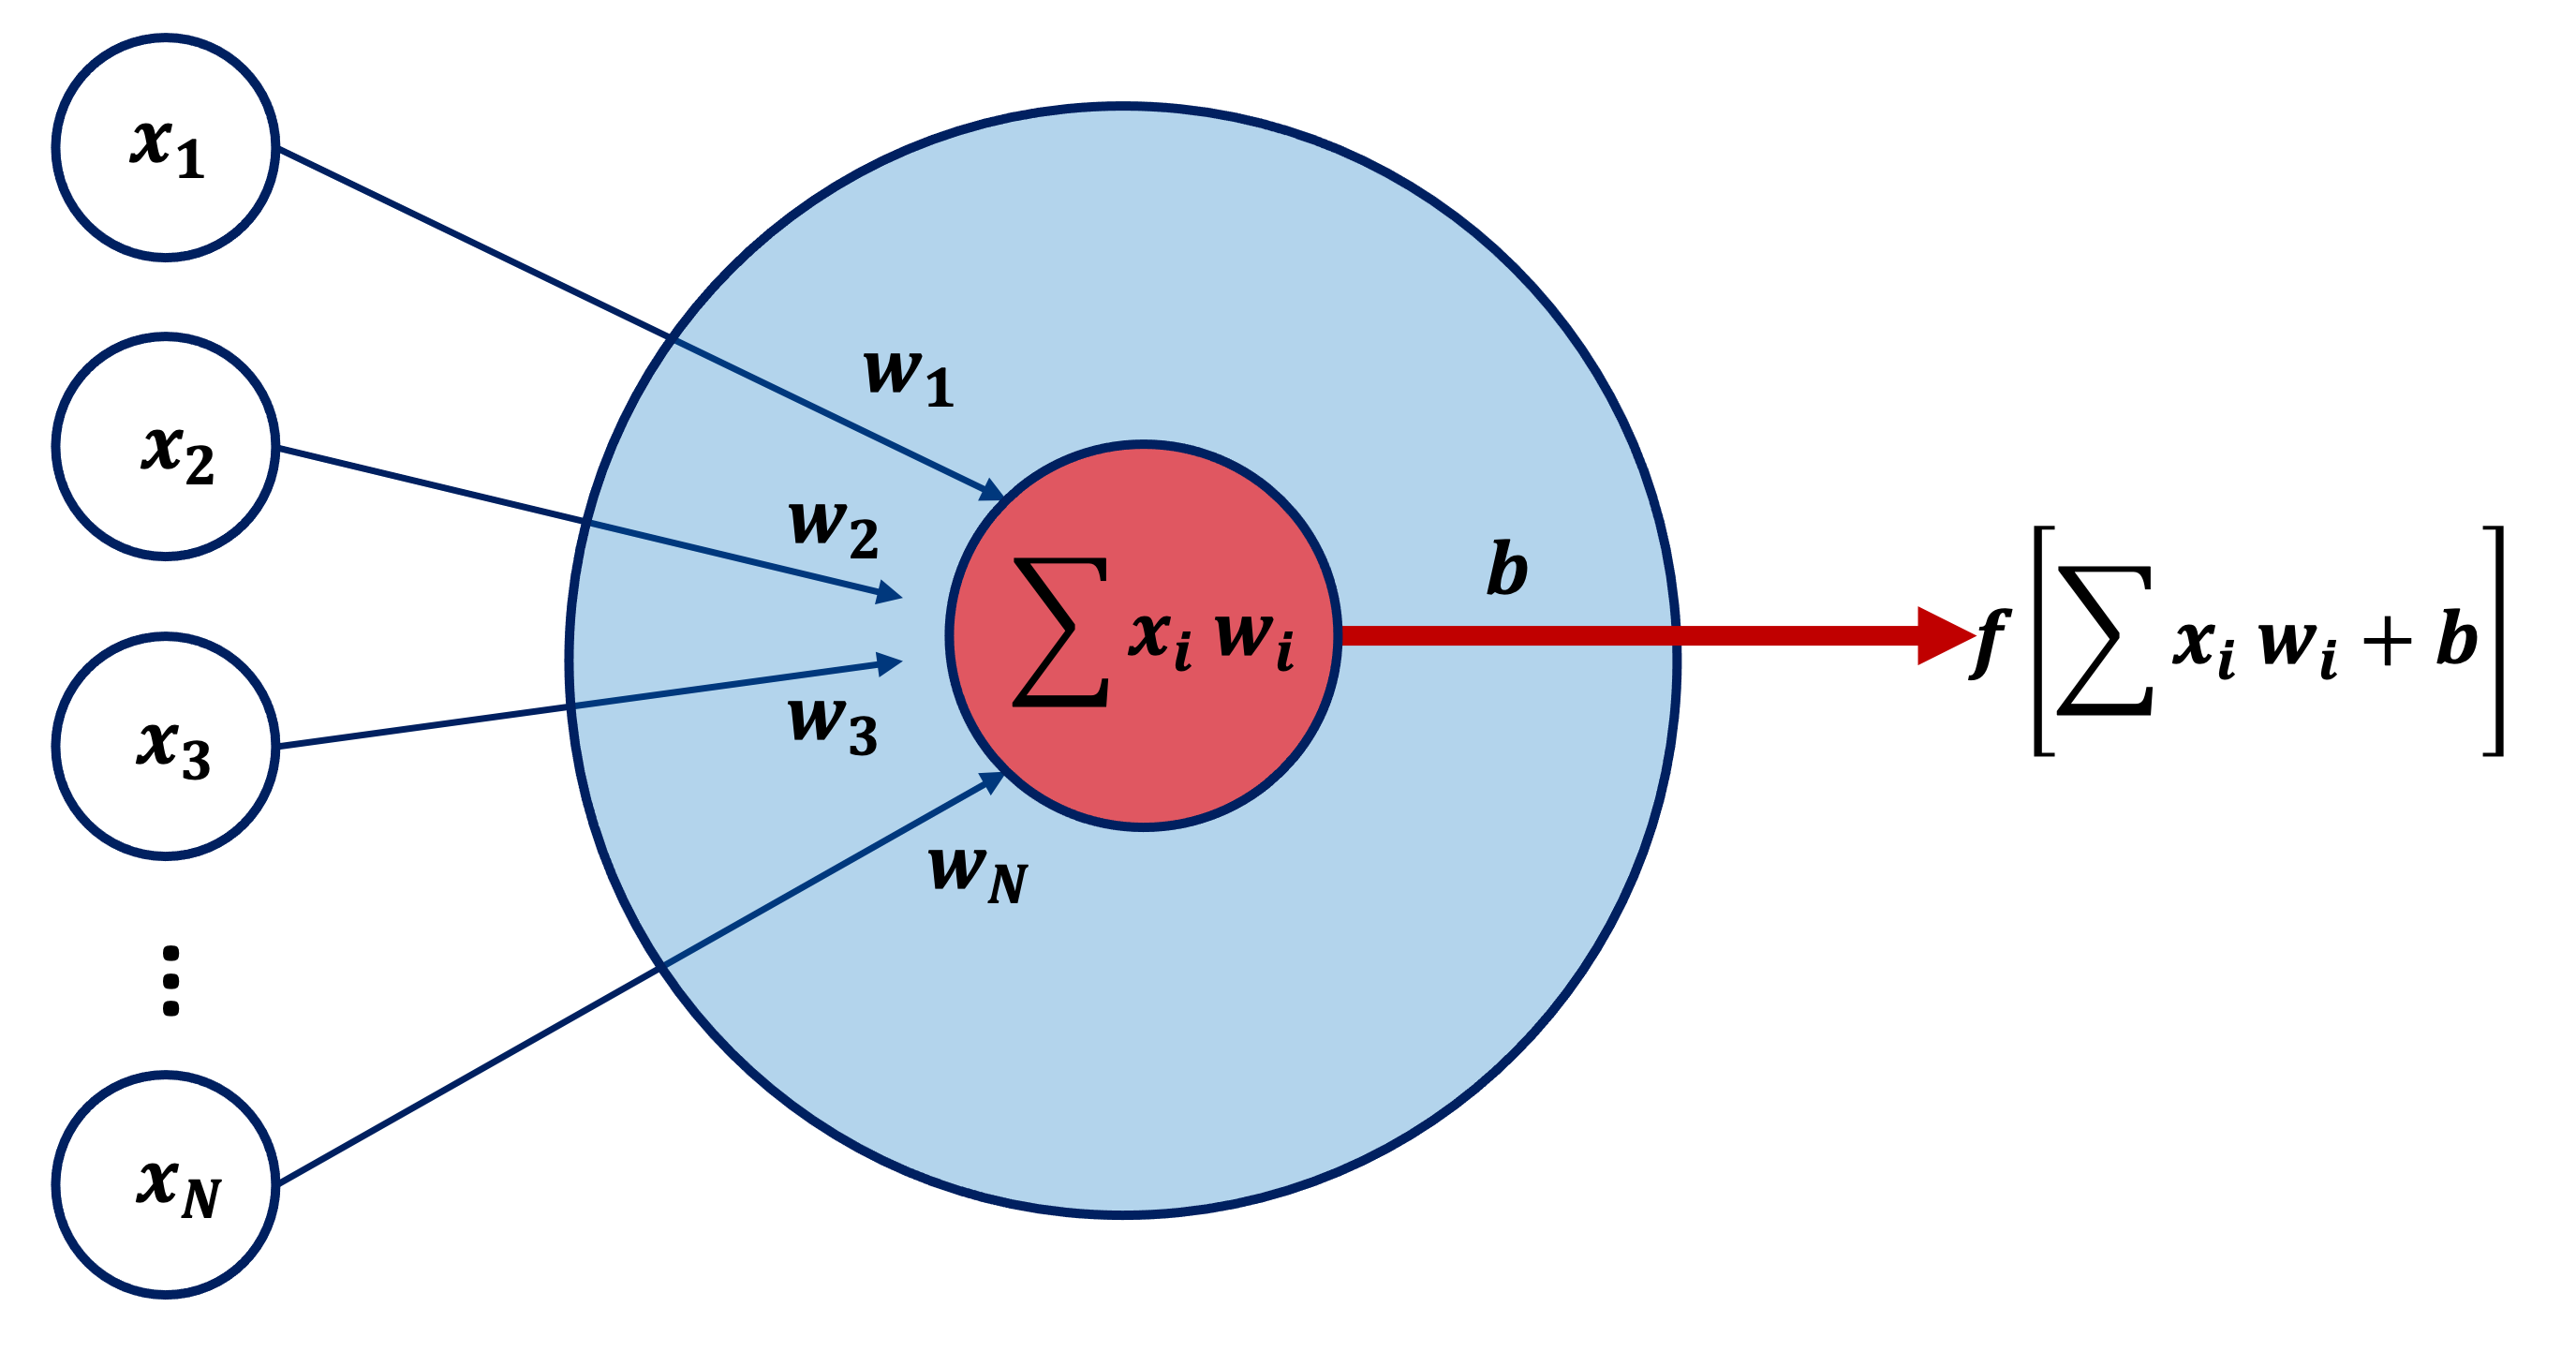
\includegraphics[scale=0.4]{Images/ML/ann.png}
    \caption{Schematics of a perceptron or an artifical neuron: the inputs $x_i$ ($i= 1, ..., N$) is multiplied by learnable weights $w_i$, summed and added a bias $b$ before being passed to an output function $f$.} 
    \label{fig:annModel}
\end{figure}

In this thesis, a \textit{perceptron} shall refer to a single artificial neuron, which is equivalent to a logistic regression model. The interest of the artificial neuron stems from a significant theoretical result: stacks of artificial neurons are \textit{universal function approximator} \cite{universalFuncApproxNN,HORNIK1989359}, as is shown in the next section on deep neural network. This theoretical result is built on a mathematically advantageous function choice for $f$: the sigmoid $\sigma$, defined in equation \ref{eq:sigmoid} and shown in Figure \ref{fig:sigmoid}:
\begin{wrapfigure}{r}{0.5\textwidth}
    \begin{center}
        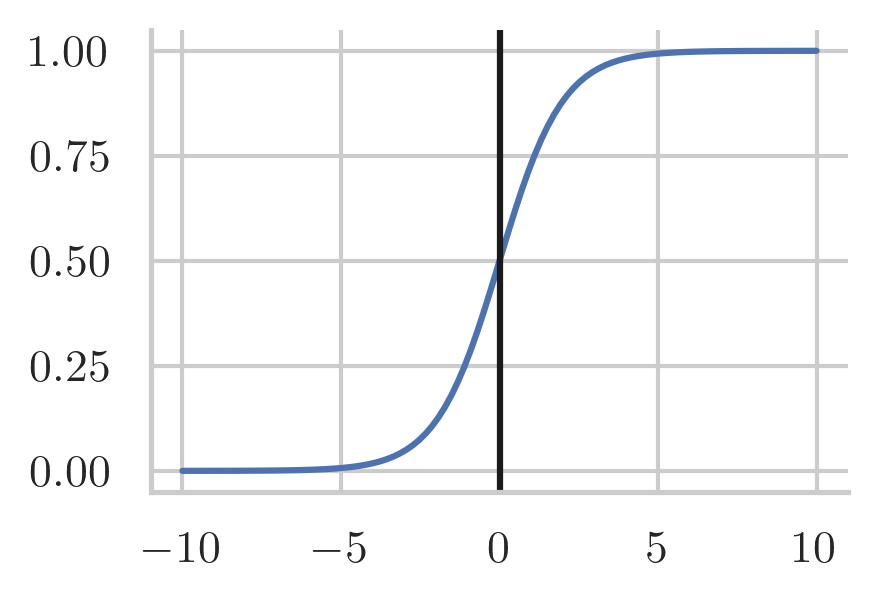
\includegraphics[width=0.35\textwidth]{Images/ML/sigmoid.png}
        \caption{The sigmoid function $\sigma$.} 
        \label{fig:sigmoid}
    \end{center}
\end{wrapfigure}

\begin{equation}\label{eq:sigmoid}
    \sigma(x) = \frac{1}{1 + e^{-x}}.
\end{equation}

Thanks to its property to map the range of real numbers to the [0, 1] range, this activation function is often used for numerical stability and to map some input to a probability distribution. A practical mathematical property of the sigmoid that is particularly relevant for \gls{dl} is the ease to compute its derivative: \[\sigma^\prime(x) = \sigma(x) (1- \sigma(x)).\]

The power of the artificial neuron comes from its ability to be efficiently combined into a well-ordered structure with powerful representation power. For an input $x \in \mathbb{R}^d$, a neuron individually applies an affine transformation $W_i^T x + b_i$, where $W_i \in \mathbb{R}^d,\,b_i \in \mathbb{R}$ are the weights and bias of the neuron $i$, that is passed through an activation function $f$ for a total output of a single neuron $f(W_i^T x + b_i)$. Combining these operations, as shown in the next section, leads to a well-structure mathematical model that has the power to represent all well-behaved continuous functions. 

\subsection{Deep Neural Networks}
A Deep Neural Network (\gls{dnn}), also called Multilayer Perceptron (\gls{mlp}), \gls{ann}, \gls{nn}, or feed-forward neural network, is made by stacking layers of artificial neurons as shown in Figure \ref{fig:neuralnet} Each neuron in a layer receives as input the output of each neuron of the previous layer, and connects to each neuron of the next layer. Layers of artificial neurons that are placed between the input and output are said to be \textit{hidden layers}. The particularlity of the design of this architecture is that layers of neurons connect to all neurons of the next layers only, defining a feed-forward computation graph from input $x$ to output $y$. Mathematically, a single layers at depth $i$ with $m$ units given as input the previous layer of dim $n$ at depth $i-1$ computes the  transformation of Equation \ref{eq:feedforward}

\begin{equation}\label{eq:feedforward}
    a^i = f^i\left({W^i}^T a^{i-1} + b_i\right),
\end{equation}
where $W^i \in \mathbb{R}^{m \times n}$ is the matrix of weight of layer $i$ - one row per unit of layer $i$, one column per unit of layer $i-1$, $b_i \in \mathbb{R}^m$ is the vector of bias, one per unit of layer $i$, $f^i$ is the activation function of layer $i$, and $a^{i-1} \in \mathbb{R}^n$ are the $n$ activated output of layer $i-1$. Note that strictly speaking the activation could be different for the units of the layer but is often unique per layer to accelerate matrix computations with vector operations.

\begin{figure}[h!]
    \center
    \begin{minipage}[l]{0.38\textwidth}
        \caption{A deep neural network with $d$ layers of width $m$, $l$ ..., $k$. Each artificial neuron, represented by a ball of darkening blue along depth, computes an affine transformation of the input of the layer followed by an activation function. The input of the \gls{dnn} is $x$ and the output is $y$.} 
    \label{fig:neuralnet}
      \end{minipage}
      \begin{minipage}[c]{0.6\textwidth}
        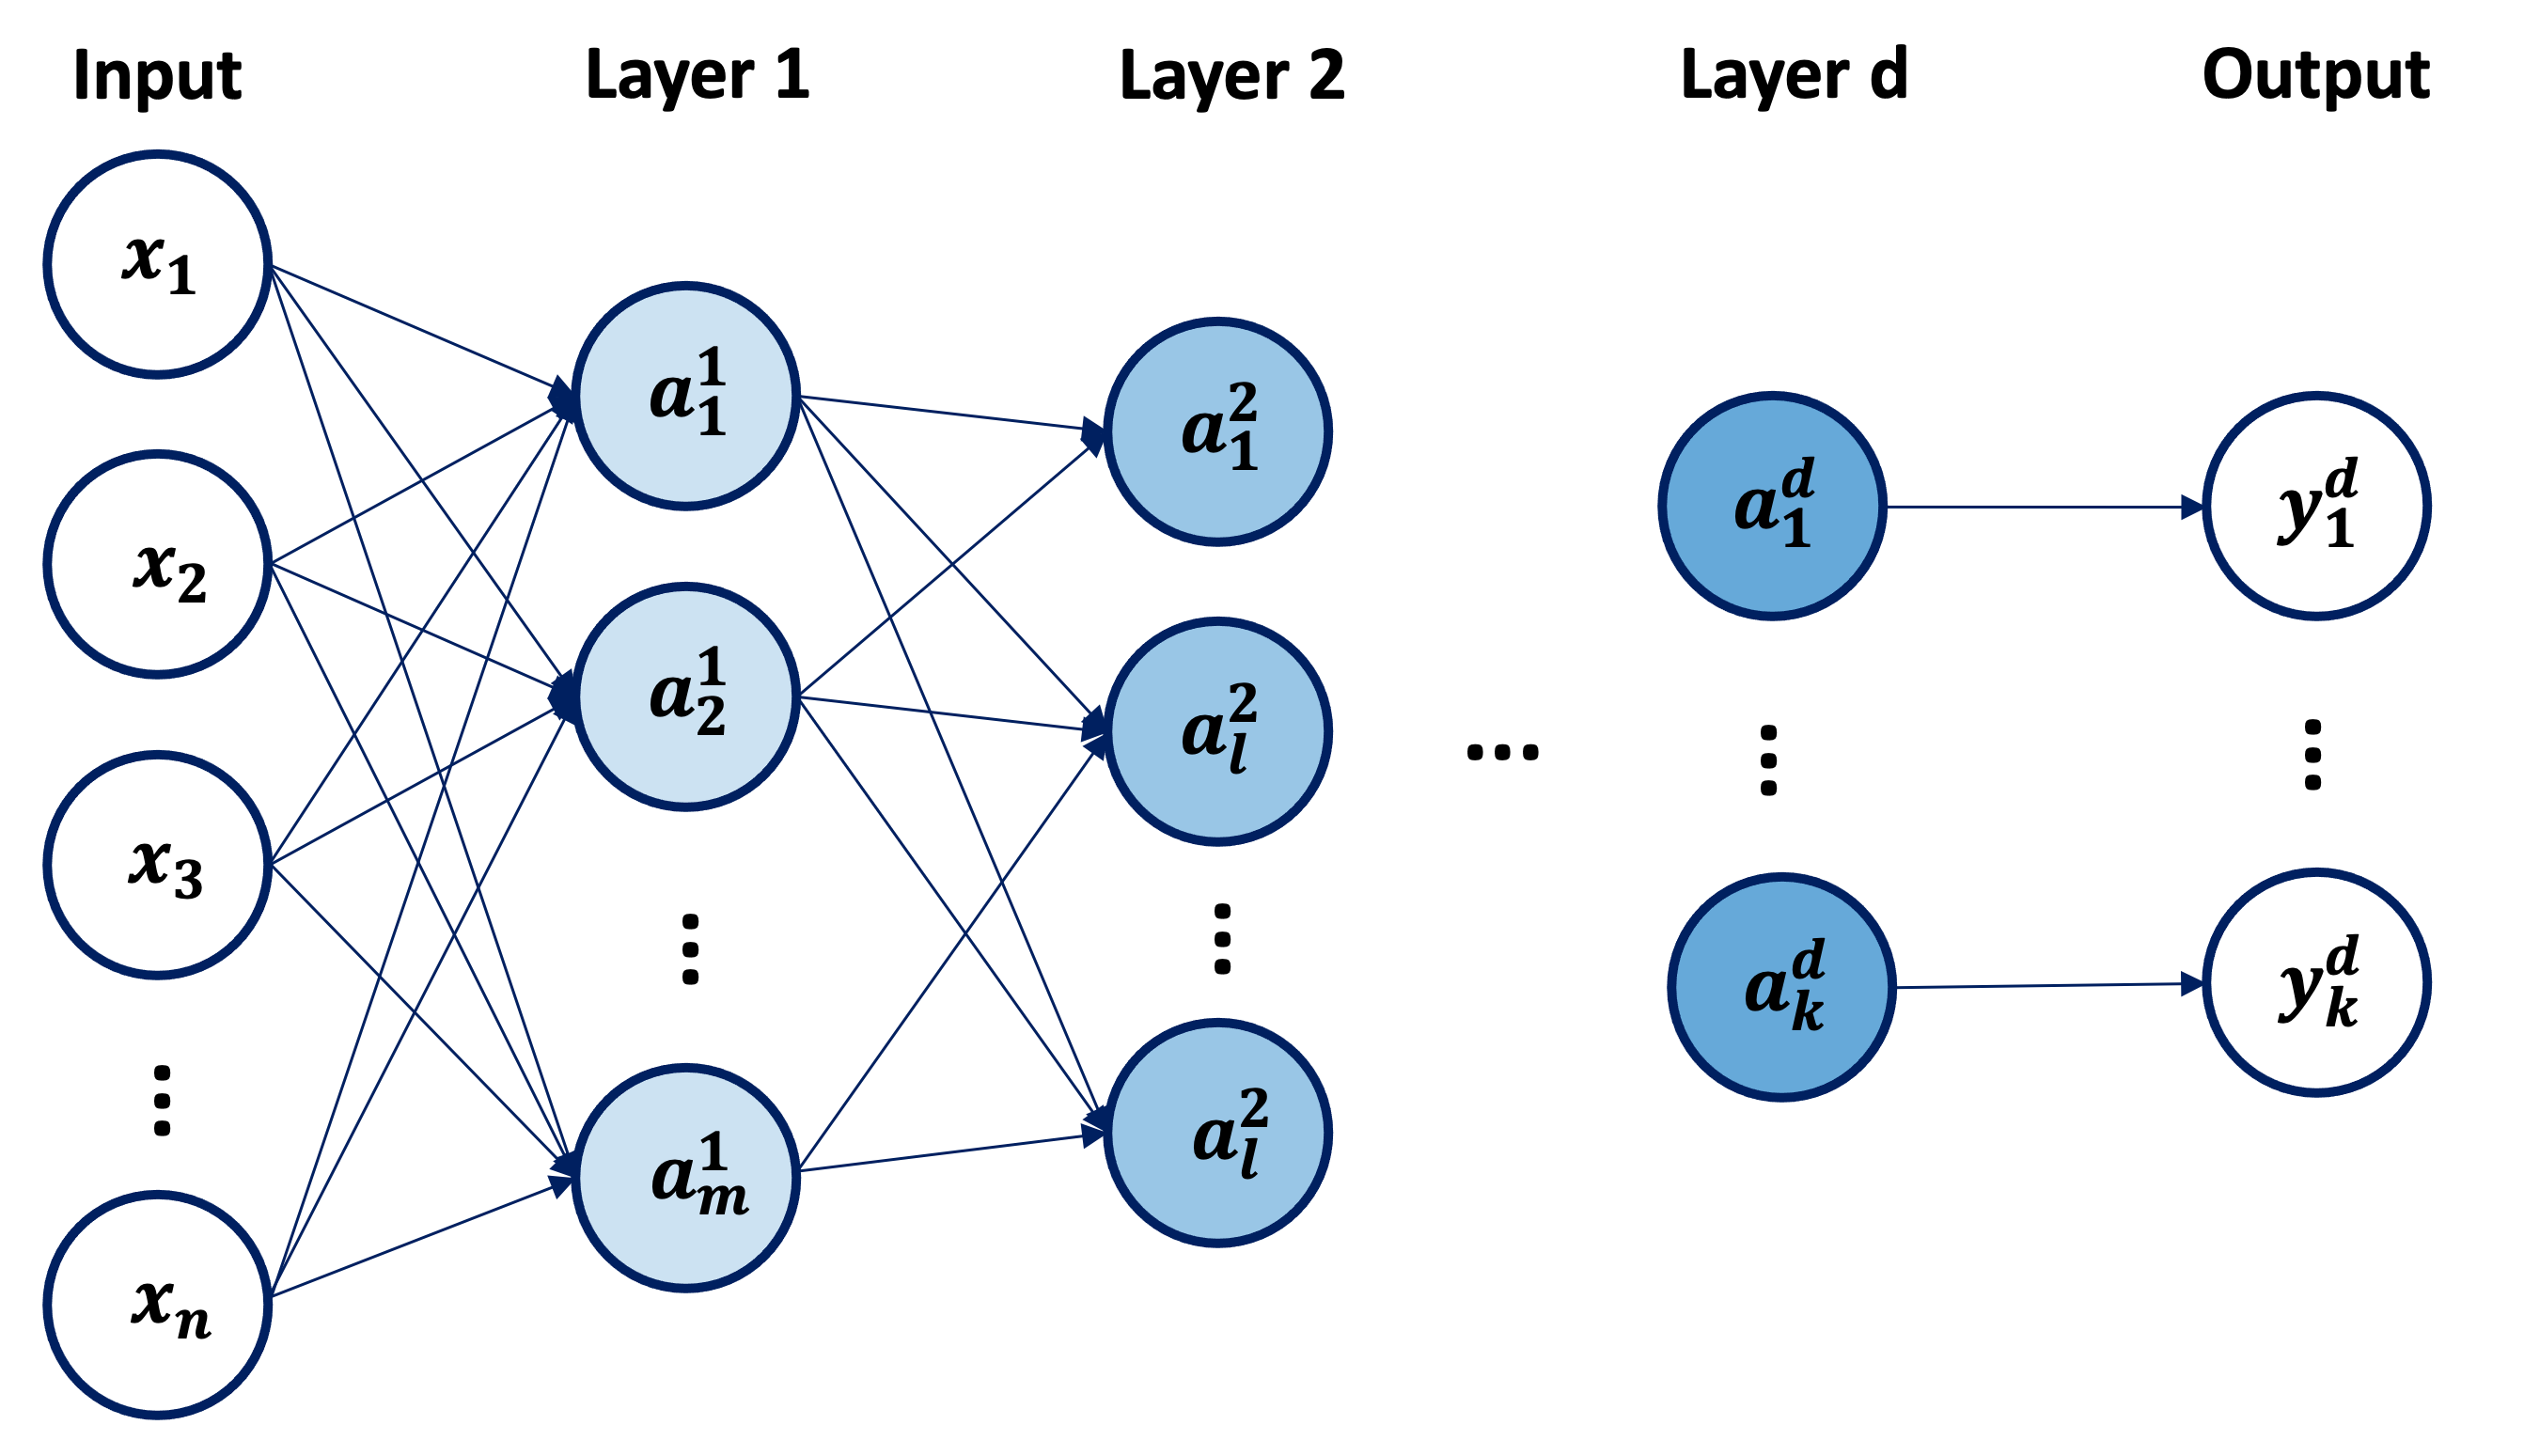
\includegraphics[width=\textwidth]{Images/ML/neuralnet.png}
      \end{minipage}
\end{figure}

Neural networks implement a system computing combination of Equation \ref{eq:feedforward}. A powerful theoretical motivation for neural networks stems from the fact they are Universal Function Approximator. This theorem, or rather family of theorem depending on the type of activation $f$ considered, establishes that neural network built with appropriate activation functions are able to approximate most well-behaving functions. The most famous such theorem states \cite{universalFuncApproxNN,HORNIK1989359}:

\paragraph{Theorem:} \textit{Let $C([0, 1]^n)$ denote the set of all continuous function $[0, 1]^n \rightarrow \mathbb{R}$ and $\sigma$ be any sigmoidal activation function. Then the finite sum $f(x) = \sum_{i=1}^N \alpha_i \sigma(w_i^T x + b_i)$ is dence in $C([0, 1]^n)$. In other words, given any $f \in C([0, 1]^n)$ and $\epsilon > 0$, $\exists$ a sum $G(x)$ of the above form for which: \[ G(x) - f(x) < \epsilon \quad \forall x \in [0, 1]^n.\]}

The statement of the theorem essentially is that any function defined over the $n$-dimensional unite hypercube $[0, 1]^n$ can be approximated by an arbitrarily wide neural network. This result only requires $\sigma$ to be sigmoidal or discriminatory in the sense:
\begin{equation}
    \sigma(x) \rightarrow
    \begin{cases}
        1 \text{ if } x \rightarrow \infty,  \\
        0 \text{ if } x \rightarrow -\infty,
    \end{cases}
\end{equation}
which is, for example, satisfied by the sigmoid function. Interestingly, similar theorems were derived for other important activation function commonly used in \gls{dl}, for example for ReLu in \cite{universApproximator-Relu}. Many flavours of \gls{dnn} exist with different functions used. An important theoretical result is the requirement for the output function applied to the artificial neuron to possess some degree of \textit{non-linearity}. A neural network with strictly linear functions can indeed be seen to collapse to a linear regression model. Such a function, when applied to the output of an artificial neuron, is said to \textit{activate} it and is hence called \textit{activation functions}. The most popular such functions, shown in Figure \ref{fig:commonAct}, are:
\begin{itemize}
    \item The sigmoid function of Equation \ref{eq:sigmoid}.
    \item The hyperbolic tangent function $tanh = \frac{e^x - e^{-x}}{e^x + e^{-x}}$.
    \item The \gls{relu} function of Equation \ref{eq:relu}
    \begin{equation}\label{eq:relu}
        \text{ReLu}(x) = \text{max}(0, x),
    \end{equation}
    note that the non-linearity here is strictly between positive and negative inputs, making this activation function one of the simplest that can be leveraged in \gls{dnn} for universal function approximation. The deriviative of this function is indeed particularly easy to compute. A generalisation of \gls{relu} called leakyReLU introduces a linear function in the negative range as leakyReLu $= \max(\alpha x, x)$, with $\alpha \in [0, 1[$. 
    \item The Exponential Linear Unit (ELU) function, shown in Equation \ref{eq:elu}, modifies the Leakage \gls{relu} in the negative domain while keeping the saturation property:
    \begin{equation}\label{eq:elu}
        \text{Elu}(x) = 
        \begin{cases}
            x \quad \text{ if } x >= 0, \\
            \alpha (e^x - 1) \text{ otherwise},
        \end{cases}
    \end{equation}
    where the a hyperparameter $\alpha > 0$.
    \item The softmax function. For an $x \in \mathbb{R}^n$, the softmax return a vector softmax$(x) = [..., \frac{e^{x_i}}{Z}, ...]$ (for $i= 1, ..., N$), where $Z = \sum_i e^{x_i}$. For a 2-dimensional $x$, the softmax is equivalent to the sigmoid function. In $n$-dimension, it maps each entry of $x$ to the range $[0, 1]$ and guarantees $\sum_i $softmax$(x)_i = 1$. The softmax is therefore  helpful to define probability distributions over multidimensional outputs.
\end{itemize}

\begin{wrapfigure}{R}{0.5\textwidth}
    \begin{center}
        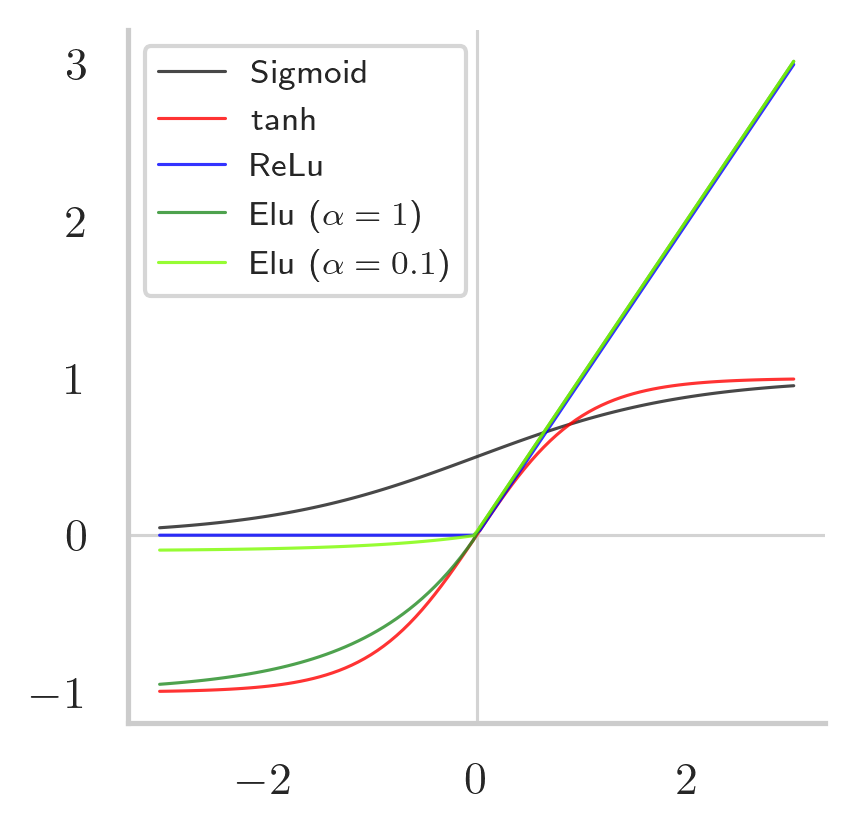
\includegraphics[width=0.45\textwidth]{Images/ML/activations.png}
        \caption{The most common non-linear activations used in deep learning.} 
        \label{fig:commonAct}
    \end{center}
\end{wrapfigure}

Many more functions have been defined in the field of \gls{ai}, with none seemingly offering a clear advantage over the ones listed here. The sigmoid is no-longer the choice of reference, due to its tendency to quickly saturates - meaning its gradient for large positive or negative input values vanishes in the sense that it tends to 0. The hyperbolic tangent $tanh$ offers larger gradients thanks to its [-1, 1]range with steeper curvature and is often the activation of choice for autoregressive architecture, such as the \gls{rnn}. The \gls{relu} function is the most widely used activation function as its derivative is extremelly efficient to compute - 1 for positive inputs and otherwise 0 - and does not suffer from vanishing gradients for positive values. Its fixed 0-value for negative input is a double edge sword: on one side, it helps the network regularises itself by deactivating neurons, on the other it could let some neurons being stuck in \textit{off}-mode if the weights are such that its pre-activation value is always negative for the input data. For this reason, it is important to correctly initialises the weights of a \gls{dnn}. An easy work around this limitation is the leakyReLu and the Elu activations, which both introduce some leakage in the negative value as controlled by a parameter $\alpha$.\\
While the Universal Function Approximator theorem gives a powerful endorsment of \gls{dl} networks, it does not state how to derive such a netowrk to fit a specific function. The task of choising the right architecture depthwise and widthwise and the correct weights and biases must be approximated by a learning strategy updating the weights and biases to reduce the error between the output and a given target. Many other data models are also Universal Function Approximators and what sets appart \gls{dl}-like models that are built on artificial neurons is the simplicity of the procedure to update their weights: thanks to their nice computational structure, under a reasonable choice of activation functions for each layer, the network is \textit{differentiable}. This means a gradient can be computed on a function measuring the difference between the target $y$ and the output $\hat{y}$ - often called a loss function when it should be minimised or a reward function when it is to be maximised - and \textit{backpropagated} across each neuron of each layer to give a local update to be applied to each individual weight and biases. The recent rise of \gls{dl} in \gls{ai} can be traced back to improvements in making this backpropagation of the gradients with publicaly available software, such as PyTorch \cite{pytorch} and TensorFlow \cite{tensorflow2015-whitepaper}, implementing efficient algorithm to perform this essential step. \\
One of the main difficulty in training a neural network is the non-convexity of the loss function as a function of the model parameters. The large number of parameters typically implemented by neural networks require large dataset to correctly assign values to the parameters without suffering from overtraining - the property to only correctly describe the data of the training set without being able to generalise the performance to data not seen during the training phase. There are two main difficulties encountered when optimising a neural network: the non-convexity of the objective function means saddle points and local minima are typically abundant and the computational complexity due to the large number of parameters makes a single update using a large dataset expensive. To circumvent these, the \textit{backpropagation} algorithm of Algorithm \ref{ag:backpropagation} is used \cite{backprop}.

\begin{algorithm}
    \caption{Backpropagation Algorithm}
    \begin{algorithmic}
    \Function{Update}{$x$, $y$, $N$, $\mathcal{L}$}
        \State Forward step: propagate input $x$ through network $N$ to get prediction $\hat{y}$
        \State Loss: compute the loss or reward of $N$: $\mathcal{L}(y, \hat{y})$
        \While{$\exists$ a layer with no gradients}
            \State Take right-most layer required a gradient
            \State Take input of layer to its right 
            \State Using the chain-rule of calculus, propagate gradient of next layer to that of current layer
            \State Store the gradient at the layer
        \EndWhile
    \EndFunction
    \end{algorithmic}
    \label{ag:backpropagation}
\end{algorithm}

In summary, the backpropagation algorithm serves as an effective way to compute \[ \frac{\partial\mathcal{L}(\theta)}{\partial\theta} = \sum_{i=1}^N \frac{\partial l(\theta)}{\partial\theta},\] 
where $\theta$ encapsulates all parameters of the model and there are $N$ datapoints, with a per datapoint loss of $l$. 
The backpropagation algorithm starts with a forward pass through the network: \[ x \xrightarrow{\times W^1 + b^1} z^1 \xrightarrow{f^1()} a^1 \xrightarrow{\times W^2 + b^2} z^2 \xrightarrow{f^2()} a^2 \xrightarrow{\times W^3 + b^3} ... \xrightarrow{\times W^d + b^d} a^d = \hat{y},\] the loss is then computed $\mathcal{L}(y, \hat{y} | W^1, b^1, W^2, b^2, ..., W^d, b^d)$ before computing the gradient of each layer by starting from the right:\[\text{grad}_{W^d, b^d} = \nabla_{W^d, b^d} \mathcal{L} \rightarrow \text{grad}_{W^{d-1}, b^{d-1}} = \nabla_{W^{d-1}, b^{d-1}} \text{grad}_{W^d, b^d} \rightarrow ... \rightarrow \nabla_{W^{1}, b^1} \text{grad}_{W^2}, \]
where the operation $\text{grad}_{W^{d-1}, b^{d-1}} = \nabla_{W^{d-1}, b^{d-1}} \text{grad}_{W^d, b^{d}}$ implies a use of the chain rule to obtain the local gradient, based on information already obtained. In the context of \gls{dl}, the chain rule of multivariate calculus offers a transformation:
\begin{equation}
    \frac{\partial h}{\partial x} = \frac{\partial h}{\partial z}\frac{\partial z}{\partial x},
\end{equation}
for a function $h: \mathbb{R}^n \rightarrow \mathbb{R}^m$, composiong two functions $h = g \circ f$ defined as $f: \mathbb{R}^n \rightarrow \mathbb{R}^k$, $g: \mathbb{R}^k \rightarrow \mathbb{R}^m$, with $x \in \mathbb{R}^n$ and $z = f(x) \in \mathbb{R}^k$. Two types of updates are necessary: 
\begin{itemize}
    \item For a layer $l$, the activation can be unpacked: \[\frac{\partial l}{\partial z^l} = \frac{\partial l}{\partial a^l} \frac{\partial a^l}{\partial z^l}\]
    \item For a layer $l$ having access to next layer $l+1$ $(\frac{\partial l}{\partial z^{l+1}})$: \[\frac{\partial l}{\partial z^l} = \frac{\partial l}{\partial z^{l+1}} \frac{\partial z^{l+1}}{\partial z^l} = \frac{\partial l}{\partial z^{l+1}} \frac{\partial z^{l+1}}{\partial a^l} \frac{\partial a^l}{\partial z^l}, \] but since $z^{l+1} = W^{l+1}a^l + b^{l+1}$, this reduces to:\[\frac{\partial l}{\partial z^l} = \frac{\partial l}{\partial z^{l+1}} W^{l+1} \frac{\partial a^l}{\partial z^l}, \]

    \item Combining the two above, we can compute $\frac{\partial l}{\partial z^l}$ for each layer in backward order. One thus now requires the derivative with respect to the per-layer weights: \[\frac{\partial l}{\partial W^l} = (a^{l-1} \frac{\partial l}{\partial z^l})^T,\] 
    
    for the weight matrix - an outer product between a row vector $\frac{\partial l}{\partial z^l}$ and a column vector $a^{l-1}$. For the bias: \[\frac{\partial l}{\partial b^l} = \frac{\partial l}{\partial z^l},\] the result is directly obtained from the row vector. 
\end{itemize}

Once all the gradients are locally available, the next step is to update all the parameters to reduce the loss by taking a step in the direction opposed to the gradient, giving the largest reduction in loss. For example for a specific parameter $w_{ij}$ at training step $t+1$:
\begin{equation}\label{eq:gradientdescent}
    w^{T=t+1}_{ij} \leftarrow w^{T=t}_{ij} - lr \times \text{grad}\left[w^{T=t}_{ij}\right],
\end{equation}
where the \textit{learning rate} $lr$ controls how large a step is taken in the opposite direction of the gradient. Since the gradient of the earlier layers will be derived from the gradient of later layers, it is important for the gradients to respect some numerical stability to avoid the risk of vanishing gradient ($\rightarrow$ 0) or exploiding gradients ($\rightarrow \infty$). This requires some care in the architecture choice and might motivate the use of a specific activation function over another. Note that strictly speaking, the activation function needs not be a continuous differentiable function ($C^1$), as the existence of a right or left derivative is sufficient, hence the function should at least be continuous ($C^0$). \\
Concerning the loss function $\mathcal{L}$, there is a lot of freedom in how to set it up - although it should be differentiable - and some typical choices are:
\begin{itemize}
    \item The cross-entropy loss function - also called the logistic loss - is based on the notion of entropy, as defined in Equation \ref{eq:statEntropy}, and is often used to assign probabilities in a classification with $c$ classes: \[ -y_i \log\hat{y}_i,\] where $y_i$ is the real label of the datapoint and $\hat{y} \in [0, 1]^C$ is the model prediction, respecting $\sum_i \hat{y}_i = 1$. Given the requirements on the output, it is typically combined with a softmax. 
    \item the Mean Squared Error (MSE): \[\frac{1}{N}\sum_i^N (y_i - \hat{y}_i)^2.\] 
    \item the Mean Absolute Error (MAE): \[\frac{1}{N}\sum_i^N |y_i - \hat{y}_i|.\]
\end{itemize} 
To regularise the model, it is common to add terms to the loss function called \textit{regulariser} in order to restric the model weights to a certain size. This can be achieved by adding to the loss $\mathcal{L}$ an L2-penalty \[\lambda \sum_i w_i^2,\] on the sum of the squared values of the weights, or an L1-penalty \[\lambda \sum_i |w_i|,\] where this last approach using the absolute value has the nice additional feature to make the network sparse - meaning to set un-necessary weights at 0. The amount of regularisation is controlled by the hyperparameter $\lambda$. Further regularisation can be obtained by randomly dropping out some connexions of the network during training, a technique called \textit{dropout} and controled by the dropout probability $p$ to incude an artificial neuron or not.

\paragraph{Pros:}
\begin{itemize}
    \item \textit{Universal Function Approximators:}
    Feedforward networks, particularly deep ones, are known to be universal function approximators. They can approximate any continuous function to arbitrary precision given sufficient hidden units and appropriate activation functions.
    \item \textit{Flexible Architecture:} The architecture of feedforward networks is flexible, allowing for customization in terms of the number of layers, the number of neurons in each layer, and the choice of activation functions. This flexibility makes them suitable for various tasks.
    \item \textit{Feature Learning:} Feedforward networks can automatically learn hierarchical representations of features from the input data. This is beneficial for tasks where the underlying patterns are complex and not easily captured by handcrafted features.
    \item \textit{Non-linearity Handling:} By introducing non-linear activation functions, feedforward networks can capture and model non-linear relationships in data, enabling them to solve more complex problems compared to linear models.
    \item \textit{Availability of Optimisation Techniques:} Various optimisation techniques, such as gradient descent and its variants, are well-suited for training feedforward networks. This makes it possible to efficiently update the network weights during the training process.
\end{itemize}

\paragraph{Cons:}
\begin{itemize}
    \item \textit{Limited Modeling of Sequential Data:} Feedforward networks are not naturally designed for handling sequential data and temporal dependencies. \gls{rnn} and Transformer architectures are often preferred for tasks involving sequential information.
    \item \textit{Fixed Input Size:} Traditional feedforward networks have a fixed input size. While techniques like padding or resizing can be employed, they might not be suitable for handling inputs of varying lengths in tasks like natural language processing.
    \item \textit{Lack of Memory:} Feedforward networks do not have an inherent memory mechanism, which can be a limitation when dealing with tasks requiring the model to retain information over a sequence of inputs.
    \item \textit{Vanishing and Exploding Gradients:} Training deep feedforward networks can be challenging due to the vanishing and exploding gradient problems. Gradients may become too small or too large during backpropagation, leading to difficulties in learning deep representations.
    \item \textit{Need for Sufficient Labelled Data:} Feedforward networks often require a large amount of labelled data for effective training. In domains where labelled data is scarce, the performance may be limited.
\end{itemize}

This section introduces deep neural networks, the simplest feed-forward architecture constituted of artificial neurons stacked into layers to generate an output $y$ based on an input $x$. There are many refinements to this base architecture, and some are explored in the next sections. 

\subsection{Recurrent Neural Networks}\label{sec:RNN}
The first modification to the \gls{dnn} considered in this thesis are Recurrent Neural Networks (\gls{rnn}). These models were derived to work with sequences, such as occuring in natural language processing. The main change with the \gls{dnn} architecture is in the way information is passed through the network: \gls{rnn} are autoregressive models. The information flow is bidirectional: the computation sequentially processes through the same structure the input at given step with the output of the prior step. The advantage of this representaton is that this cyclical flow can be unfolded into a direct acyclical computational graph that, for a given sequence length, is equivalent to a \gls{dnn} pass. Figure \ref{fig:rnnNet} presents the structure of an \gls{rnn}-based network as well as its unfolding. The input $x$ is a sequence of $N$ tokens, and the length of different inputs $x_i$ in the dataset can vary. The mathematical structures implemented by this architecture to generate an output $y$ of length equal to the input is that of Equation \ref{eq:rnnModel} for the step $t$ ($t=1, ..., N$):
\begin{equation}\label{eq:rnnModel}
    y_t = W(h_t) = W(V(x_t) + U(h_{t-1})),
\end{equation}
where $U$, $V$, and $W$ are three, potentially different, \gls{dnn}s mapping taking at timestep $t$ respectively the previous hidden state $h_{t-1}$, the current input token $x_t$ and the new hidden state $h_t = V(x_t) + U(h_{t-1})$. The initial hidden state $h_0$ is usually initiated from a special mapping from the whole input $x$. An interesting feature of such a network is its ability to build an internal memory of previous inputs up to a timestep $T$ thanks to the chain of hidden states $h_{t<T}$. To avoid having too large (exploding) or small (vanishing) gradients, which would not correctly update the weights of the model during gradient descent, the $\tanh$ function is often used as activation in \gls{rnn} thanks to its smooth distribution and limitation to the range $[-1, 1]$. Unfortunately, due to the network relying on repetitive multiplications of numbers in the range $[-1, 1]$, the effect of much earlier timestep ($h_{t<<T}$) can be lost when processing later input at $T$. This process is referred to as \textit{memory loss}. Thankfully, there are many main architectural modifications to \gls{rnn} that improve their operational memory, of which the two main ones are \gls{lstm} and \gls{gru}.

\begin{figure}[h!]
    \center
    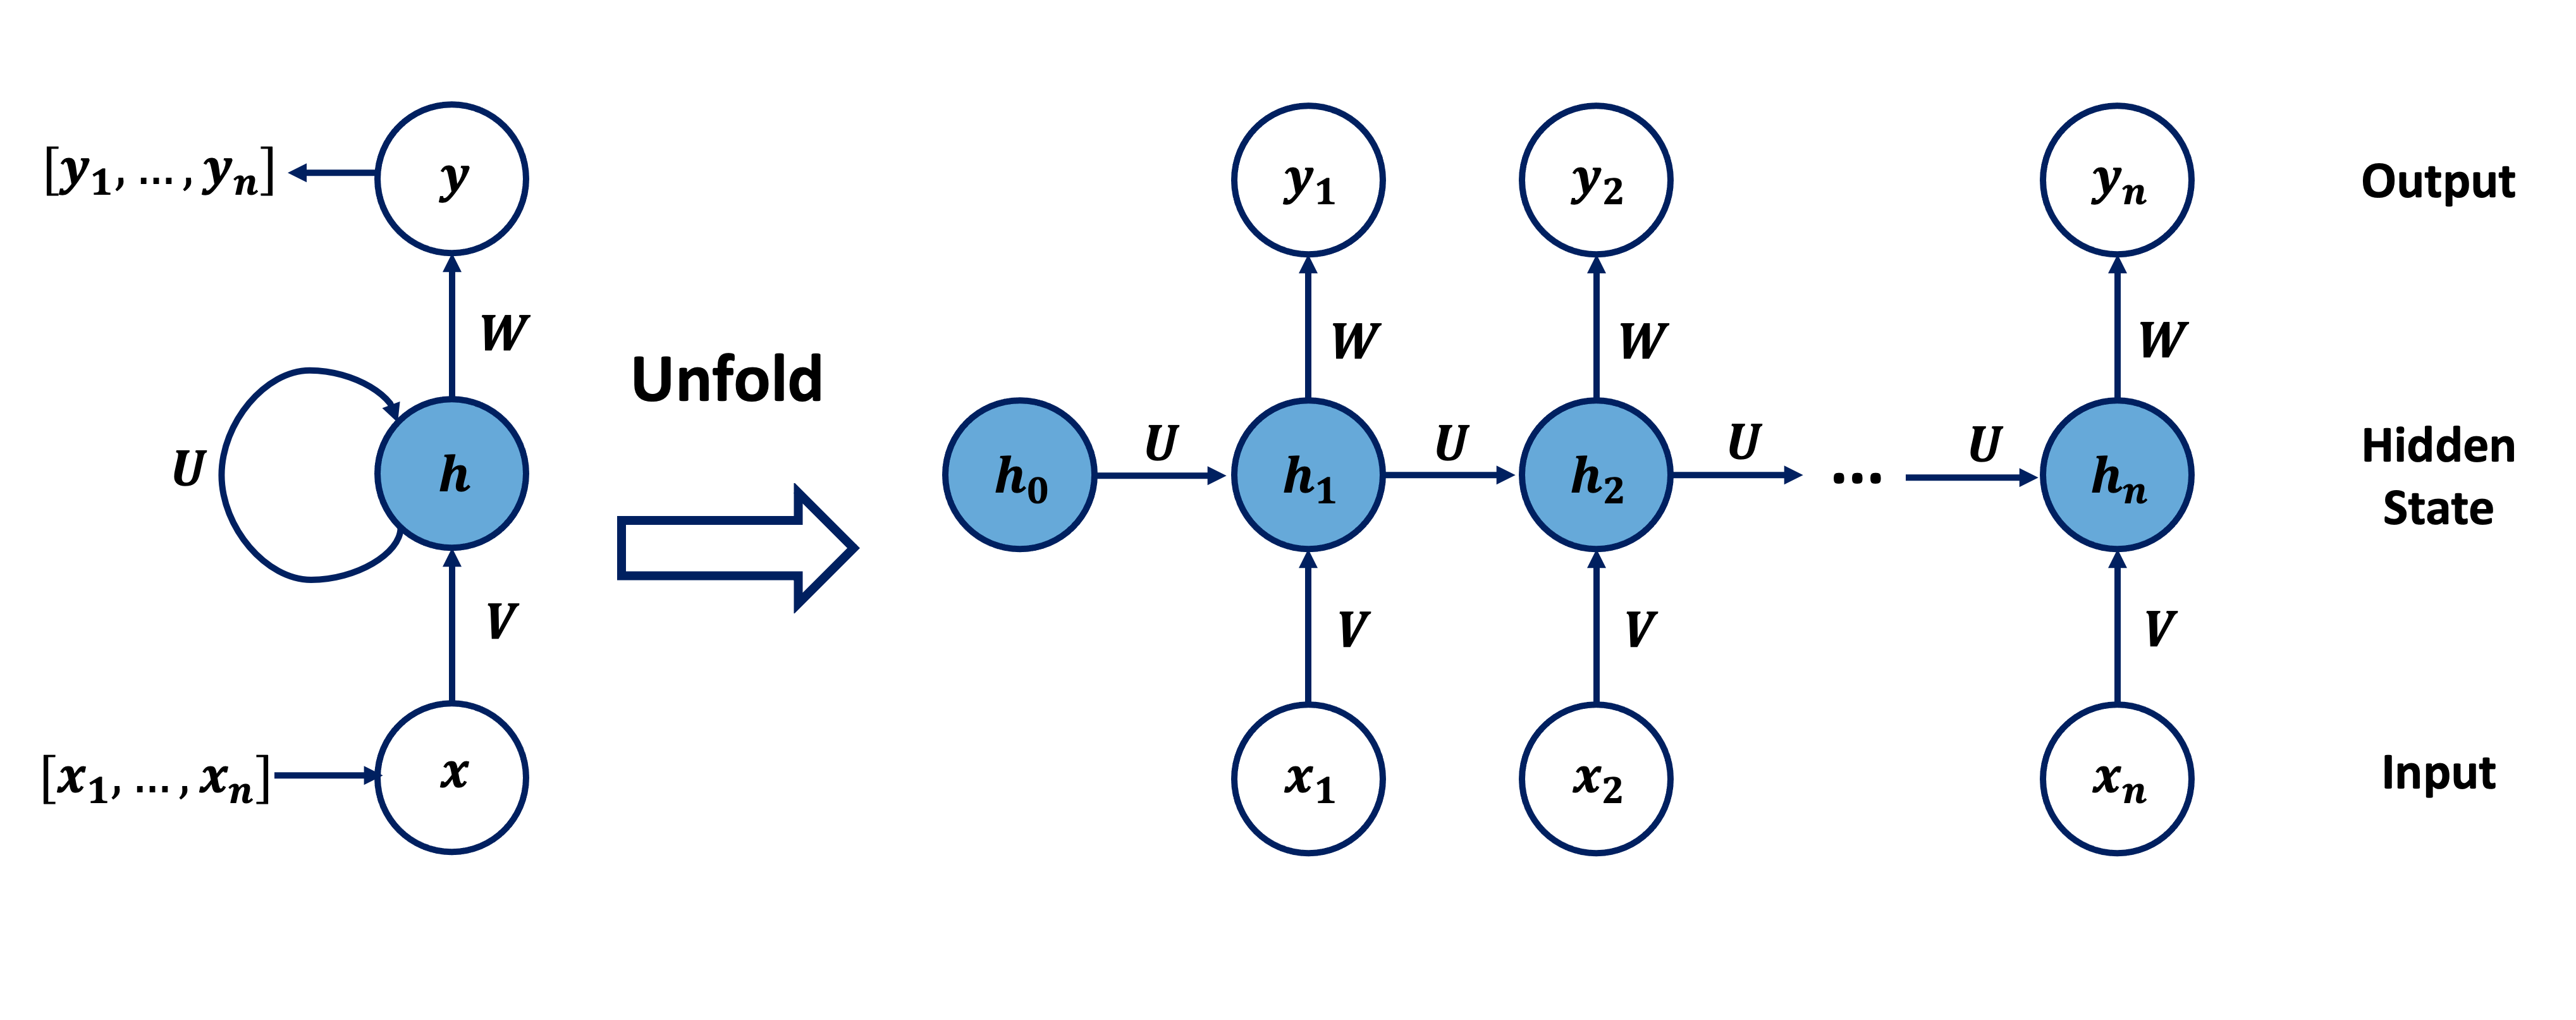
\includegraphics[scale=0.5]{Images/ML/rnn.png}
    \caption{A recurrent neural network, using 3 feed-forward neural networks (DNN) $U$, $V$, $W$, to map the input sequence $x = [x_1, x_2, ..., x_N]$ to the output $y = [y_1, y_2, ..., y_N]$ using the internal hidden state $h^t$ evovling for each timestep $t$. $h_0$ would typically be obtained by a mapping of the whole input sequence $x$. } 
    \label{fig:rnnNet}
\end{figure}

\subsubsection{Long-Short Term Memory} 
As shown in Figure \ref{fig:lstmCell}, Long-Short Term Memory (\gls{lstm}) cells implement a specific architecture to propagate information along the sequence, with the introducion of a new control state $c$ \cite{lstmPaper}. Three gates covering the forget, the input, and the output regulate the flow of information from the cell. In particular, the forget gate $F$ decides what information to keep from prior states, by multiplying these values by a factor 1 and discards the rest through a multiplication by a factor close to 0. The input gate $I$ is tasked with creating the new internal state of the cell and what information to store in it. Finally, the output gate $O$ decides what information in the cell should be brought to the output. This selectivty of the \gls{lstm} cell to decide what to use from memory, what to keep in memory, and what to output give this architecture a much improved memory for long sequences which result in a much improved efficiency. 

\begin{figure}[h!]
    \center
    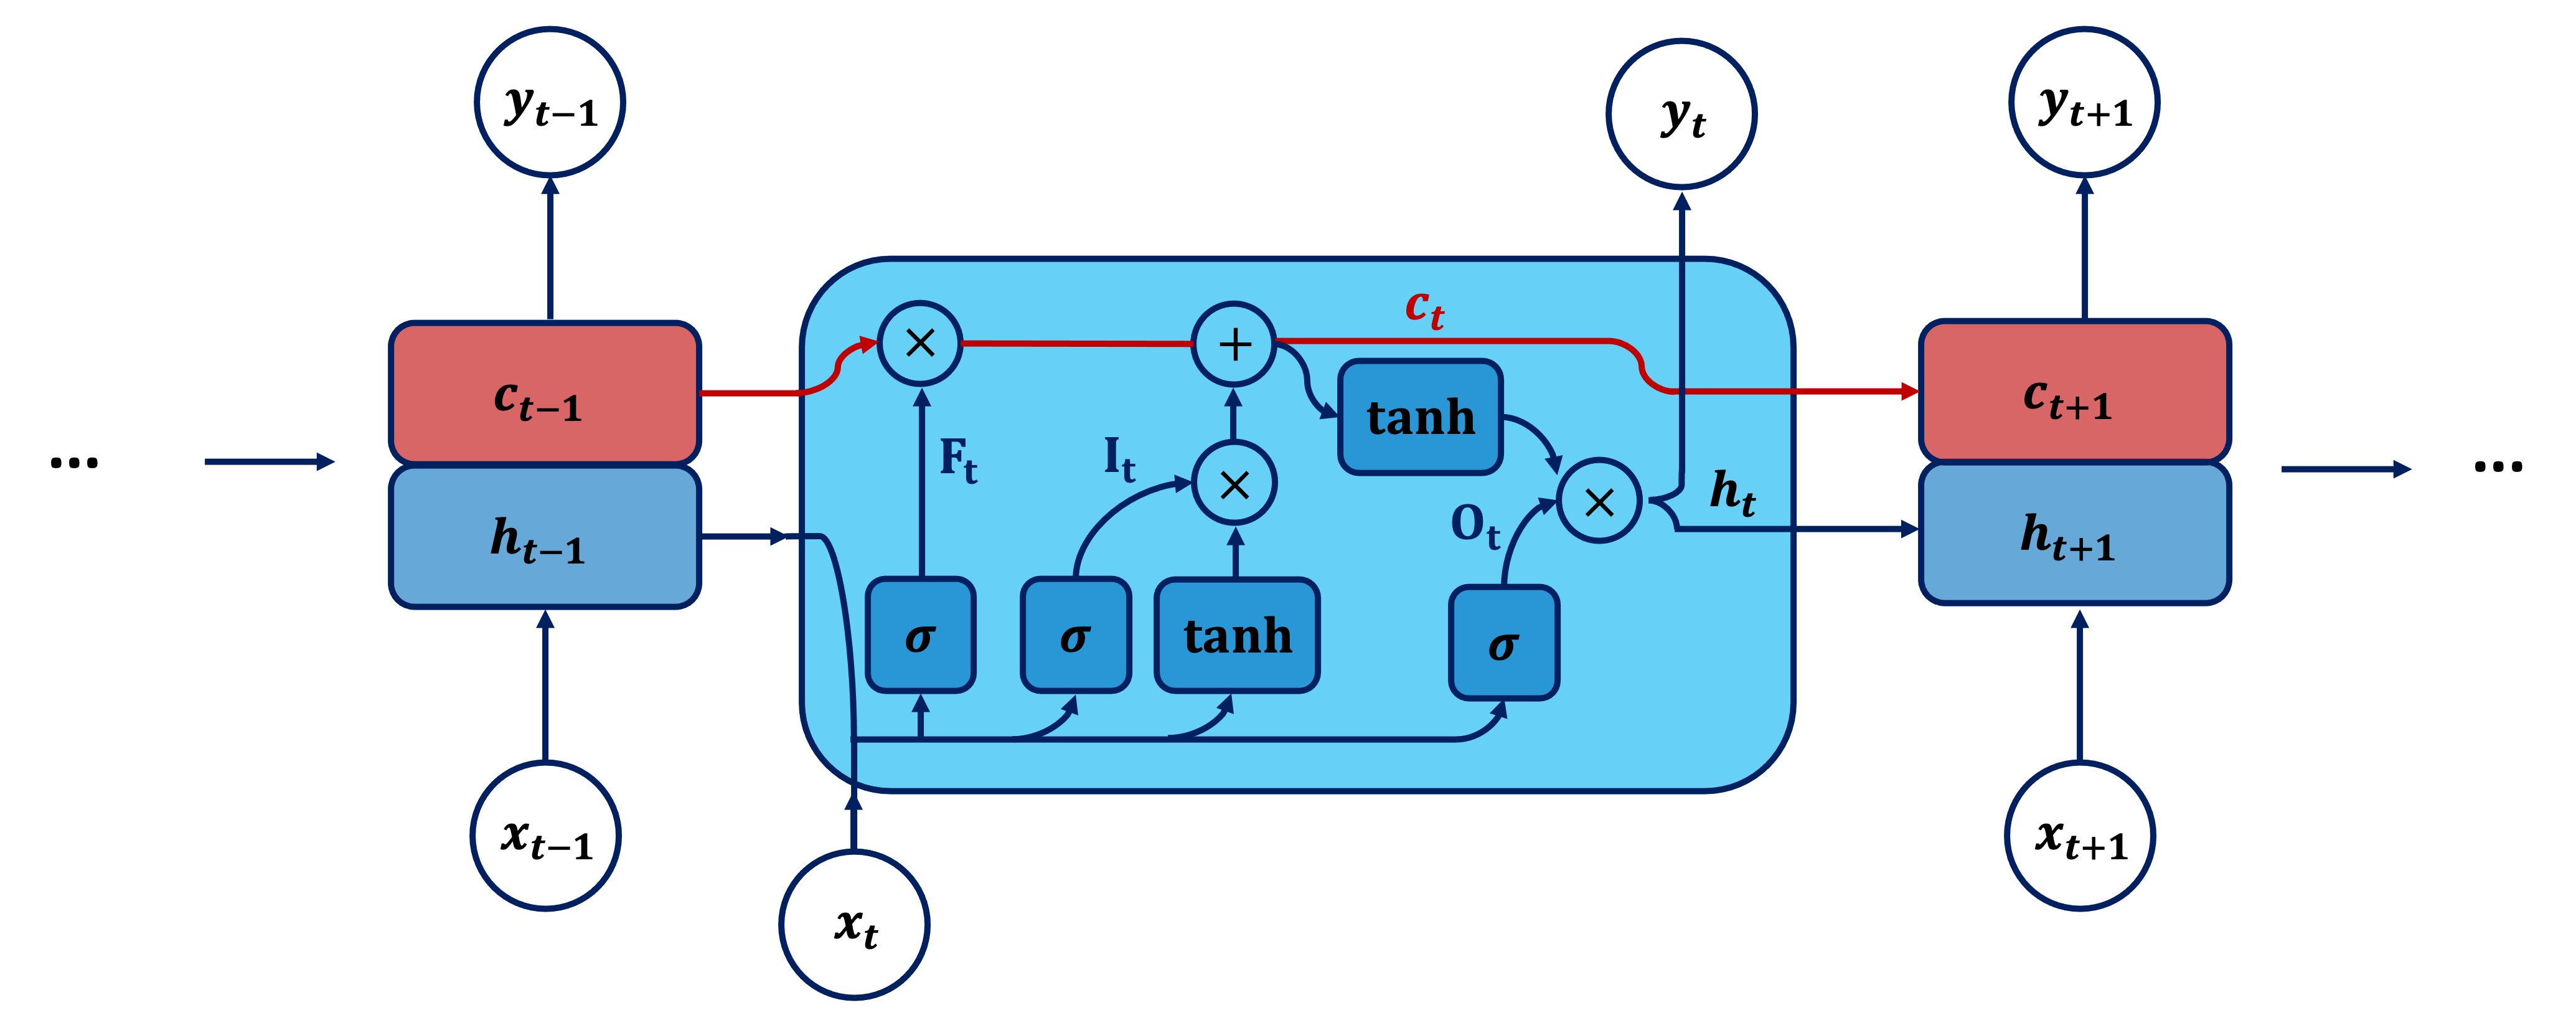
\includegraphics[scale=0.5]{Images/ML/lstm.png}
    \caption{An LSTM cell. Arrows and lines that merge imply concatenation of the inputs, the $\times$, $+$, and tanh are element-wise operation and the $\sigma$ are different layered transformations (1-layer feed-forward network). $F_t$ is the forget gate of the memory cell $c$, $I_t$ the input gate, and $O_t$ the output gate. } 
    \label{fig:lstmCell}
\end{figure}

\subsubsection{Gated Recurrent Unit} 
The Gated Recurrent Unit (\gls{gru}) is another adventageous design to improve the memory of a recurrent-like network without using as many parameters as an \gls{lstm} \cite{gruPaper}. There is no output gate and only one internal hidden state $h_t$ is required. This architecture comes in different version, with the fully gated version presented in Figure \ref{fig:gruCell}. It only requires two gates: the \textit{update gate} $Z$ and the \textit{reset gate} $R$. The former lets the model decide how much of the past information should be kept and the latter is used to forget past information.

\begin{figure}[h!]
    \center
    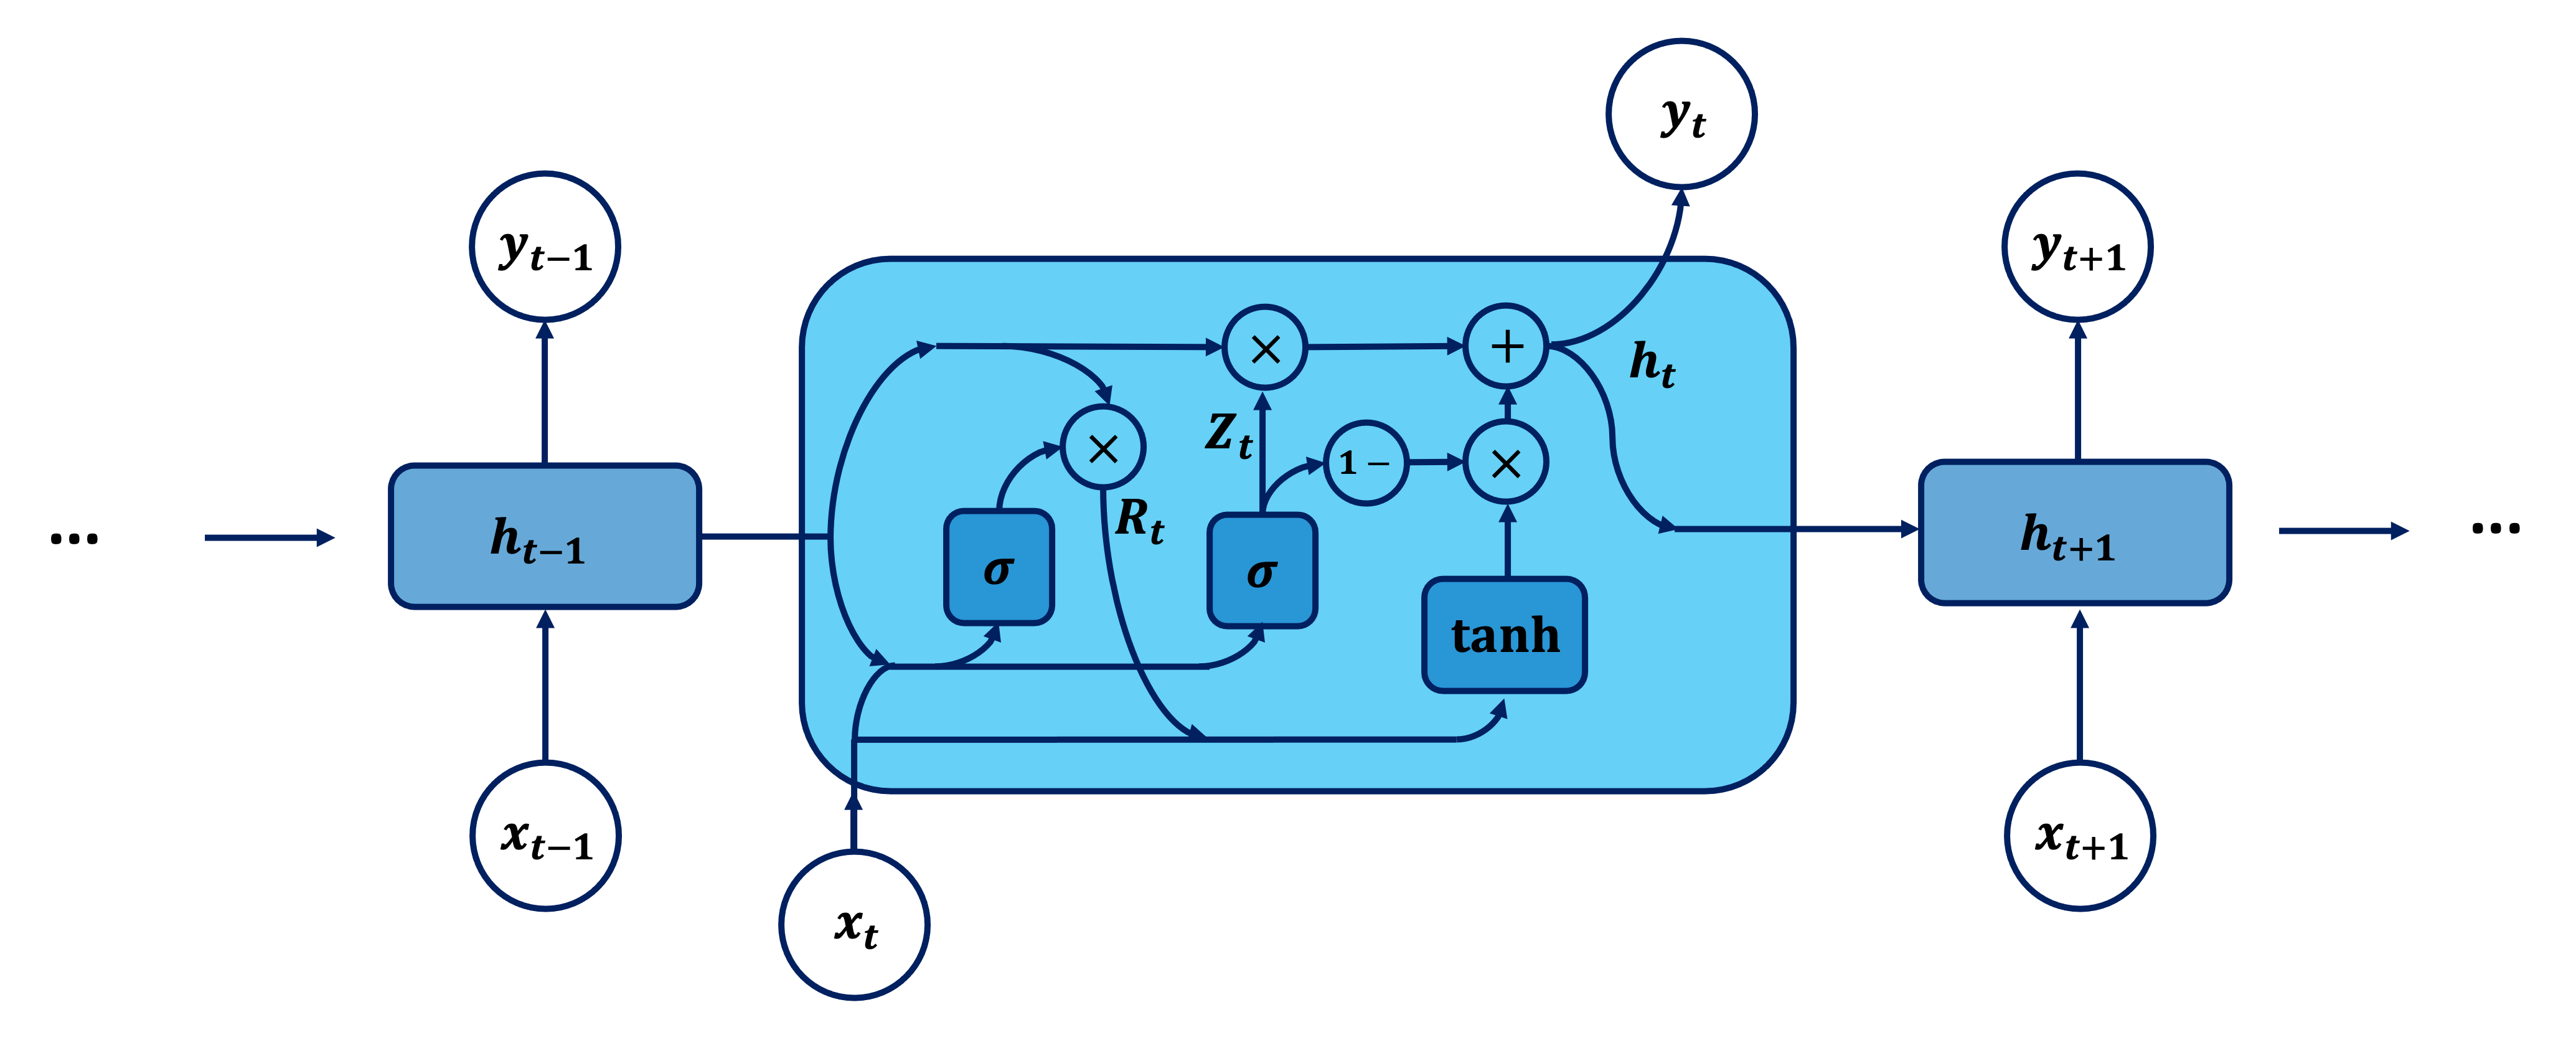
\includegraphics[scale=0.5]{Images/ML/gru.png}
    \caption{A Gated Recurrent Unit cell (fully-gated version). Arrows and lines that merge imply concatenation of the inputs, the $\times$, $+$, tanh, and ``1 - '' are element-wise operation - the last one outputting the vector 1 minus its inputs - and the $\sigma$ are two different layered transformations (1-layer feed-forward network) with sigmoid-like activation function. $Z_t$ is the update gate and $R_t$ the reset gate. } 
    \label{fig:gruCell}
\end{figure}

\gls{rnn}s and their modification have been designed for ordered sequence analysis and have had great results in such settings. Ordered sequences are natural in language analysis, where a sentence such as \textit{``the boy hit the car''} is meaninguflly different to its permutation \textit{``the car hit the boy''}. The choice to sequentially analyse the tokens of a sequence with memory lets \gls{rnn}-based operates simularly to a Turing Machine, endowing them with the powerful representational flexibility of Universal Turing Machine \cite{NEURIPS2021_ef452c63}. A significant drawback however is the impossibility to fully parallelise the analysis of the sequence due to its strict ordering, making \gls{rnn}s expensive models to train even on highly parallelised hardware. The main motivation behind the Transformer design, introduced in section \ref{sec:transformer}, was to fix this crucial weakness. \\

\paragraph{Pros:}
\begin{itemize}
    \item \textit{Sequential Processing:} \gls{rnn} are designed to handle sequential data, making them suitable for tasks with temporal dependencies.
    \item \textit{Flexibility:} \gls{rnn} can operate on input sequences of variable length.
    \item \textit{Memory:} \gls{rnn} have a memory mechanism that allows them to retain information about previous inputs.
\end{itemize}

\paragraph{Cons:}
\begin{itemize}
    \item \textit{Vanishing and Exploding Gradients:} Training deep \gls{rnn} can suffer from vanishing and exploding gradient problems, affecting the learning of long-term dependencies.
    \item \textit{Limited Short-Term Memory:} Traditional \gls{rnn} struggle to capture long-range dependencies due to their limited short-term memory. 
    \item \textit{Complexity:} While \gls{lstm} and \gls{gru} architectures can mitigate the two points above, the cost is a more complex architecture that is harder to train and requires more resources. 
    \item \textit{Interpretability:} The internal workings of a \gls{rnn} is challenging to interpret.
\end{itemize}

\subsection{Convolutional Neural Networks}
Convolutional Neural Networks (\gls{cnn}) \cite{NIPS198953c3bce6, NIPS2012_c399862d} have emerged as a powerful class of deep learning models that are particularly effective in computer vision tasks, including image and video analysis. The architecture of \gls{cnn}s is roughly based on human visual processing. It consists of convolutional layers - implementing the fundamental convolution operation-, pooling layers, and feed-forward layers (\gls{dnn}). This architecture, presented in Figure \ref{fig:cnnDesign}, enables \gls{cnn} to automatically learn hierarchical representations of features while respecting properties of image-based data: spaciality (geometrical grounding), locality (neighbourhoods) and spatial symmetry.

\begin{figure}[h!]
    \center
    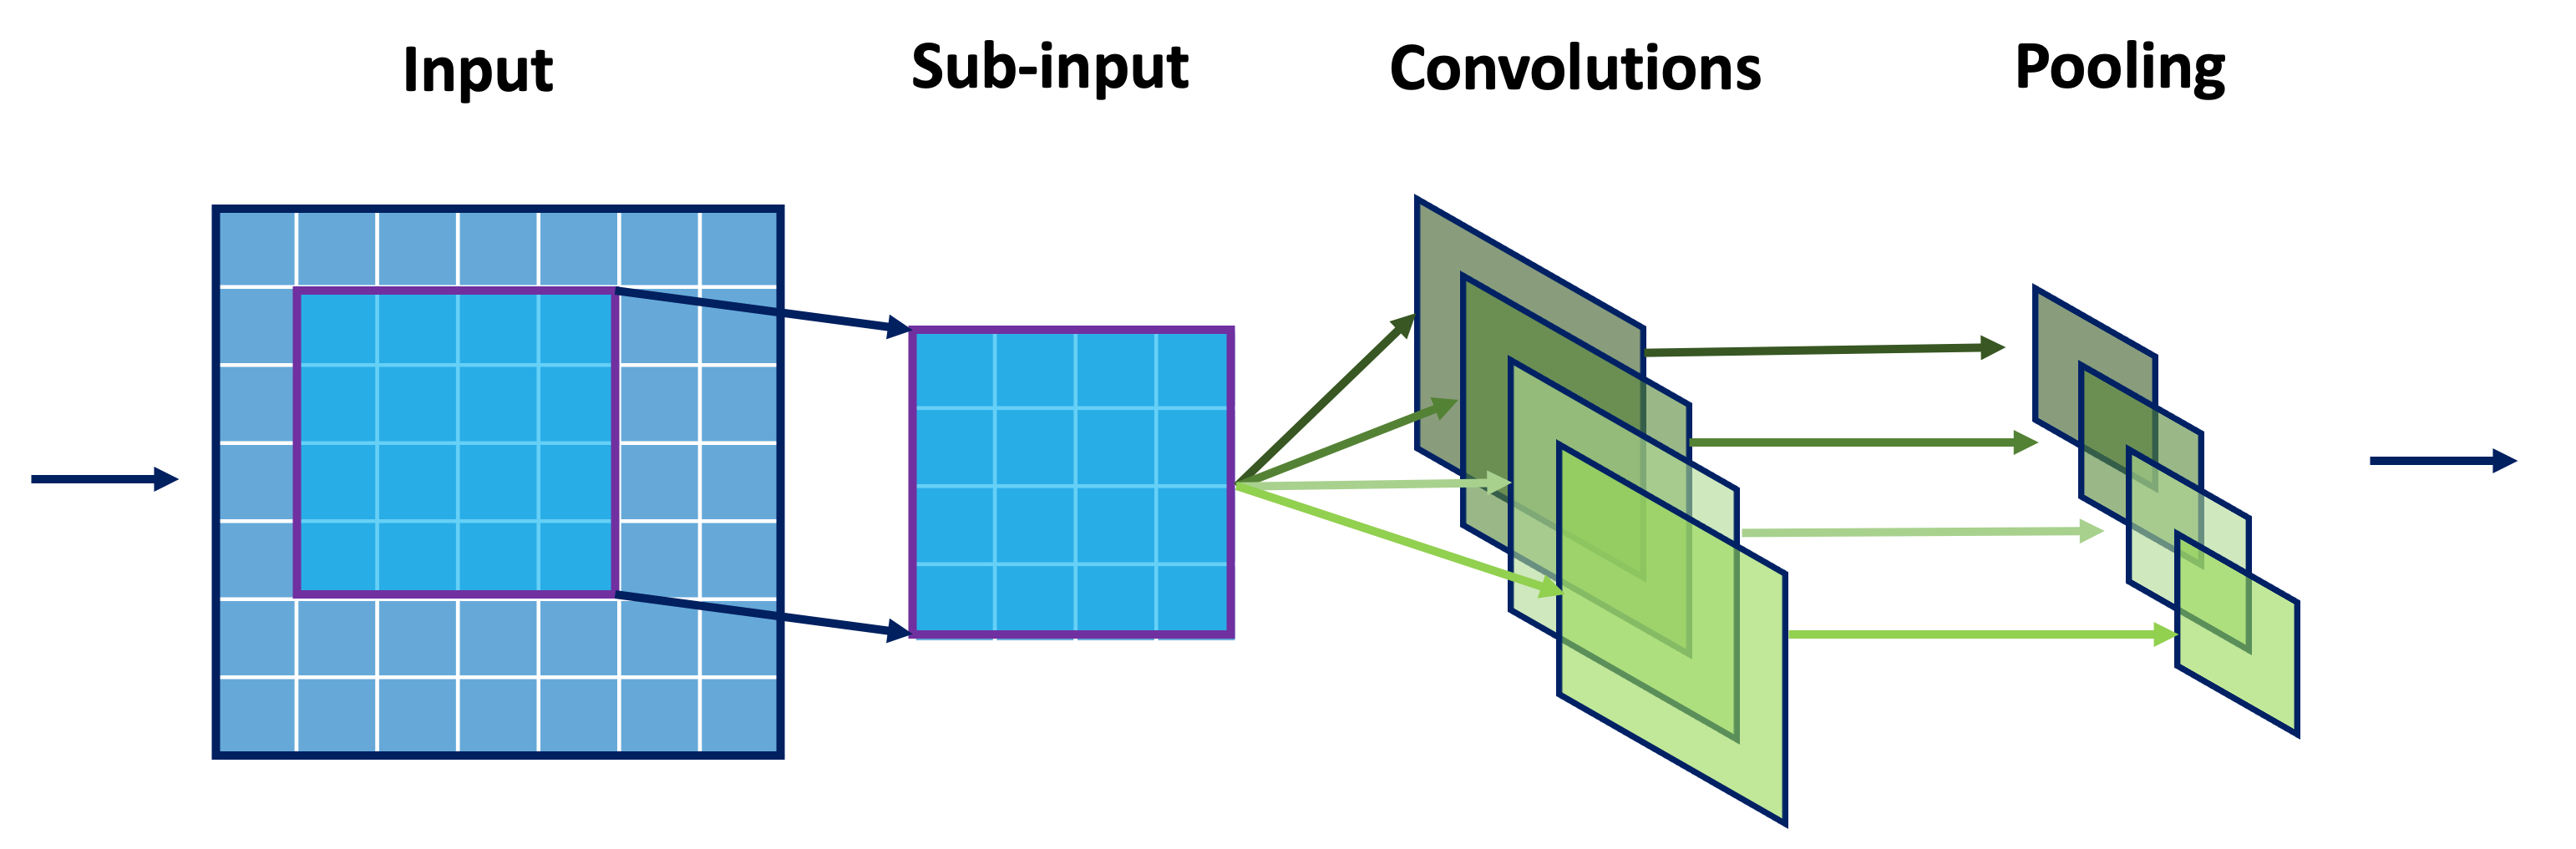
\includegraphics[scale=0.5]{Images/ML/cnn.png}
    \caption{A layer of a convolutional neural network, implementing a convolution with 4 kernels followed by a pooling operation. This design can be stacked to create deep architecture, and combined with a feed-forward neural network, after flattening the output at some depth, before reaching the final loss function layer. In this example, the receptive field size is 4 and there are 4 different kernels used to analyse an input image of size 7 $\times$ 7.} 
    \label{fig:cnnDesign}
\end{figure}

The functioning of \gls{cnn} involves the use of convolutional layers to extract local patterns and features from input data. Convolutional operations are applied to the input data by multiplying entry-by-entry a learnable \textit{kernel} or \textit{filter}, represented by a matrix of weights of smaller dimension than the total image size, with an equal size subpart of the input and applying an activation function. The size of the filter or kernel restricts the processing of the input to a given \textit{receptive field} dimension, and this window is passed over the full input image by moving it by a defined \textit{stride} length. Pooling layers are then used to reduce spatial dimensions and retain important features. This process can be parallelised for an image of multiple channel: e.g., a coloured image would be represented by a tuple of 3 values (for example, using the RGB coding) for each pixel. For classification and regression, a \gls{cnn} based model would typically stack several convolutional and pooling layers before leading to a fully connected neural network ``flattening'' the last representation to make predictions. \textit{Flattening} refers to the process of transforming the input image, represented as a matrix $\mathbb{R}^{x} \times \mathbb{R}^{y}$, into a vector $\mathbb{R}^{x \times y}$. \gls{cnn}-based models, such as AlexNet \cite{NIPS2012_c399862d} and ResNet \cite{resNetPaper}, have demonstrated state-of-the-art performance in various computer vision tasks.\\
A main advantage of the convolution operation on an image of size $x \times y$ is the reduction of the number of artificial neurons required to process the image, which helps to regularise the network.
\begin{itemize}
    \item A \gls{dnn} given the flattened image would require $x \times y$ neurons. 
    \item A \gls{cnn} with $k$ kernels of size $\alpha \times \beta$ would require $k \times \alpha \times \beta$ artificial neurons, that would be applied to different subpart of the image. 
\end{itemize}
For example, for an image of size 100 $\times$ 100, a \gls{dnn} would require 10,000 weights while a \gls{cnn} can process the image with only 25 if a single kernel of size 5 $\times$ 5 is used. Typical pooling functions are the \textit{maxPooling} or the \textit{sumPooling}, which, respectively, takes the largest element or the sum in each window of their input, with specific hyperparameters governing the size and the movements of the window.\\
\paragraph{Pros:}
\begin{itemize}
    \item \textit{Feature Learning:} \gls{cnn} automatically learn hierarchical representations of features on multidimensional data, reducing the need for manual feature engineering.
    \item \textit{Spatial Hierarchies:} Convolutional and pooling layers enable the model to capture spatial hierarchies in the input data while respecting the properties of images, namely locality: how close pixels are. 
    \item \textit{State-of-the-Art Performance:} \gls{cnn} have achieved state-of-the-art performance in image classification, object detection, and segmentation tasks.
\end{itemize}

\paragraph{Cons:}
\begin{itemize}
    \item \textit{Computational Complexity:} Training deep \gls{cnn} can be computationally intensive, requiring substantial resources.
    \item \textit{Large Datasets:} \gls{cnn} often require large labelled datasets for effective training, which may not be available for every application.
    \item \textit{Interpretability:} The internal workings of \gls{cnn} can be challenging to interpret, making them somewhat of a "black box".
\end{itemize}

\subsection{Graph Neural Networks}
In the last few years, \gls{gnn} have gained significant attention for their ability to model and analyse complex relationships within graph-structured data \cite{graphNetRef}. Originally designed for tasks such as node classification and link prediction, \gls{gnn}s have found applications in diverse domains such as social networks modelling, recommendation systems, and physics, for modelling the dynamic of a $N$-body system, performing tracks reconstruction, and identifying particles.\\
\gls{gnn}s operate on graph-structured data, where nodes or vertices represent entities, and edges represent relationships between these entities. The functioning of \gls{gnn}s involves iterative aggregation of information from neighbouring nodes and updating of the edges, allowing them to capture local and global structures as defined by the graph. This is achieved through the use of message-passing mechanisms. An interesting feature of graphs is that the input information does not need to be given a rigid structure. Consequently, graph based-methods have a much greater representation power than image- or sequence-based ones. Graphs are in fact able to represent abritrary relational structures, as defined by the graph through its directional weighted edges \cite{graphInductiveBias}. A particular feature arising from this property is that graph are permutation equivariant: the order of nodes can be rearranged without impact. \\

\begin{figure}[h!]
    \center
    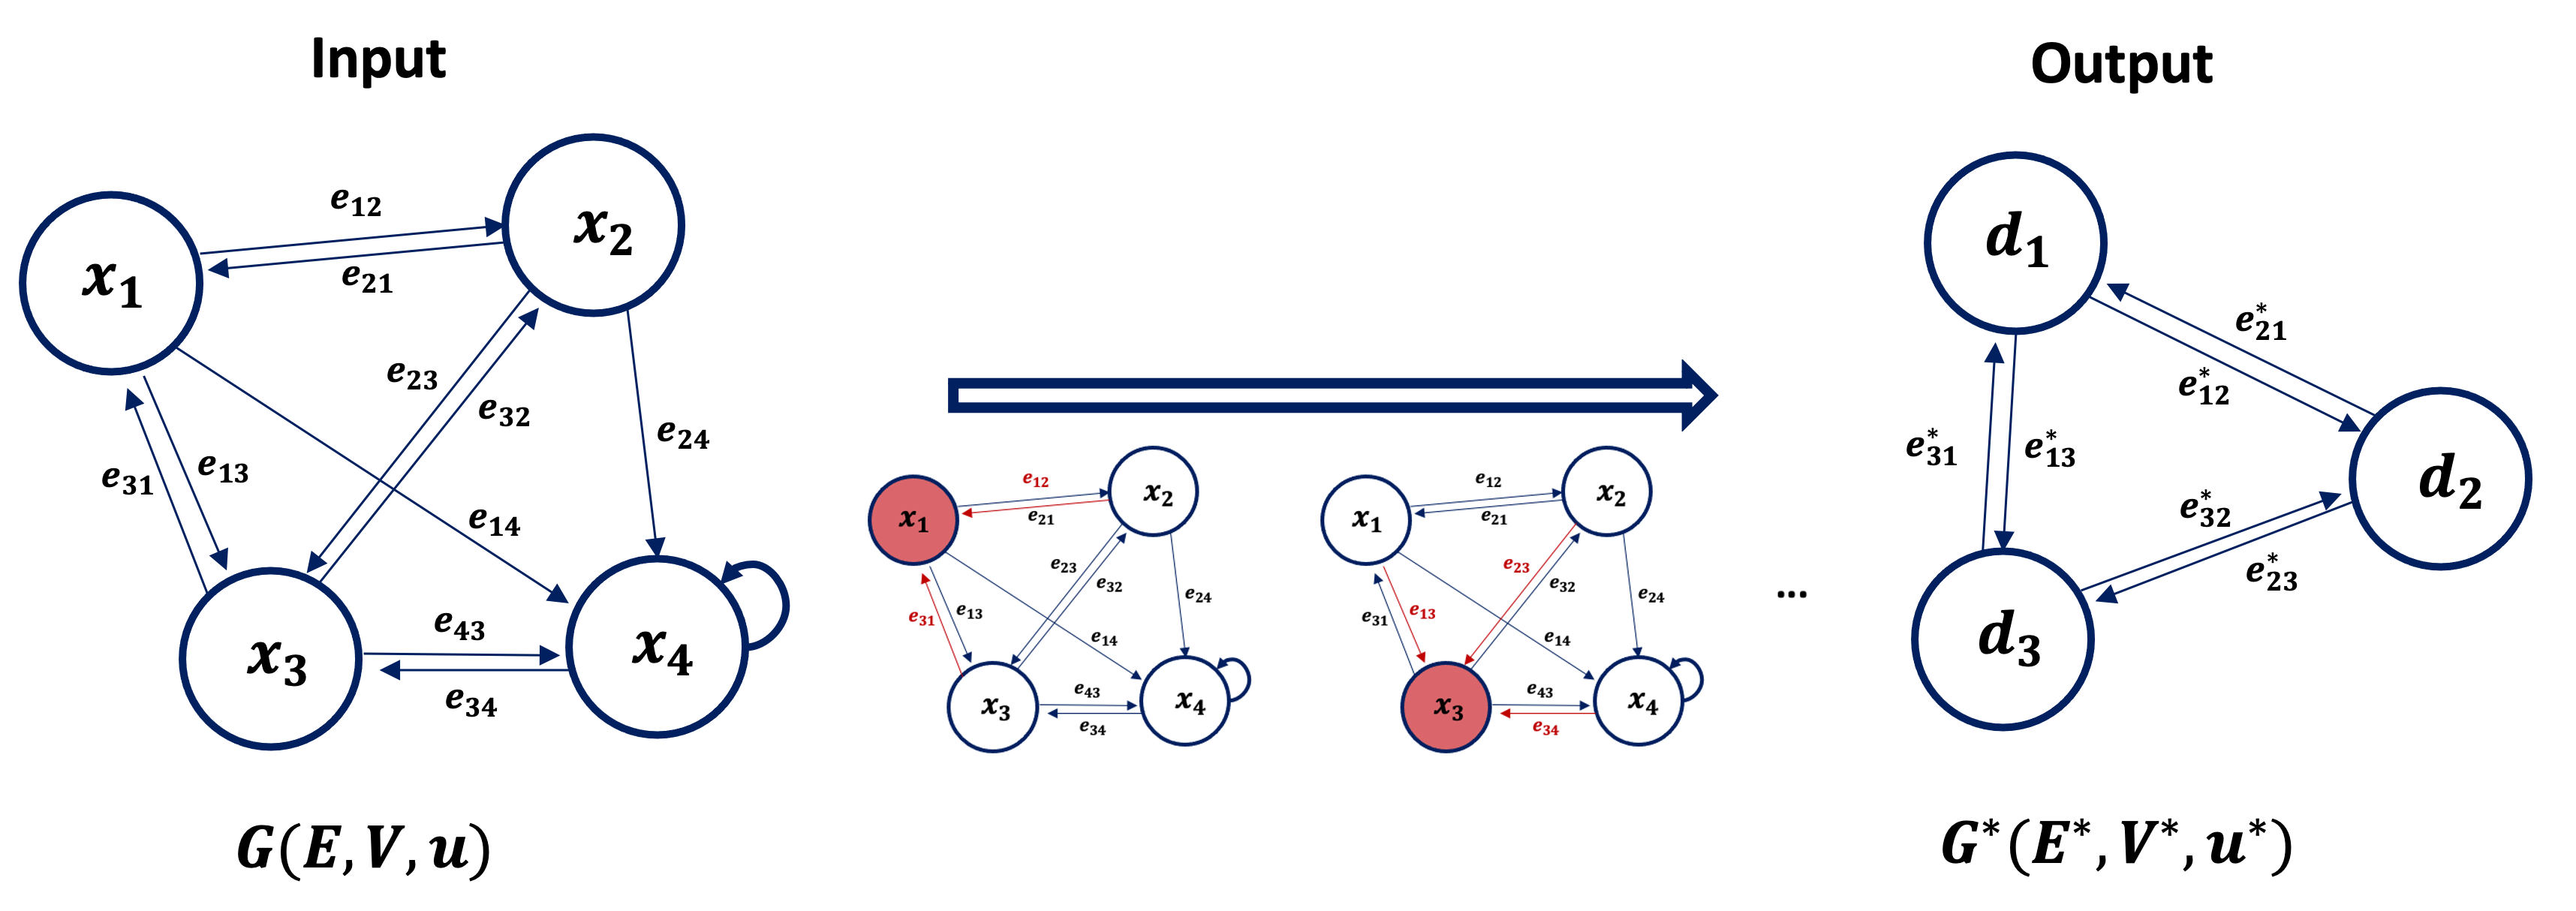
\includegraphics[scale=0.5]{Images/ML/gnn.png}
    \caption{A graph neural network update on a directed graph $G(V, E, u)$ with a global representation $u$, four initial nodes $\in V$ and edges $e_{ij} \in E$ connecting nodes $i \rightarrow j$ (in the notation of the text, each node is given a different integer index $k$ and written $(e_k, r_k, s_k)$, with $r_k = j$ and $s_k = i$). By analysing the neighbours of each node, the graph is updated to a new graph $G^*(V^*, E^*, u^*)$.} 
    \label{fig:gnnScheme}
\end{figure}

Typically, a \gls{gnn} architecture consists of multiple layers of message passing operations. Each layer updates the node representations by aggregating information from neighbouring nodes, as schematised in Figure \ref{fig:gnnScheme}. Different architectures implement different update processes for the graph, with popular \gls{gnn} architectures being Graph Convolutional Networks (GCNs) \cite{gcnPaper} and Graph Attention Network \cite{velickovic2018graph}. In this thesis, the notation adopted is to represent a graph $G$ has a tuple of three entires:
\begin{enumerate}
    \item $E = \{(e_k, r_k, s_k)\}_{k=1:N^e}$ the set of edges, with each edge having a real vector of features $e_k \in \mathbb{R}^e$ and storing the index of the receiver (sender) as $r_k$ ($s_k$).
    \item $V = \{v\}_{i=1:N^v}$ the set of nodes, each node having a real vector of features $v_i \in \mathbb{R}^v$.
    \item $u$, a global attribute of the graph modelled by a real vector of features $u \in \mathbb{R}^u$. 
\end{enumerate}

\begin{algorithm}
    \caption{Steps of Computation in a Full Graph Network Block \cite{graphInductiveBias}}
    \label{algo:graph_network}
    \begin{algorithmic}[1]
    \Function{GraphNetworkUpdate}{$E, V, u$}
        \For{$k \in \{1 \ldots N^e\}$}
            \State $e^*_k \gets \phi^e(e_k, v_{r_k}, v_{s_k}, u)$
        \EndFor

        \For{$i \in \{1 \ldots N^n\}$}
            \State Let $E_i^* = \{(e^*_k, r_k, s_k)\}$ for $k = 1 : N^e$ where $r_k = i$
            \State $\overline{e^*_i} \gets \rho^{e \to v}(E^*_i)$
            \State $v^*_i \gets \phi^v(\overline{e^*_i}, v_i, u)$
        \EndFor

        \State Let $V^* = \{v^*\}_{i=1}^{N^v}$
        \State Let $E^* = \{(e^*_k, r_k, s_k)\}_{k=1}^{N^e}$
        \State $\overline{e^*} \gets \rho_{e \to u}(E^*)$
        \State $\overline{v^*} \gets \rho_{v \to u}(V^*)$
        \State $u^* \gets \phi_u(\overline{e^*}, \overline{v^*}, u)$

        \State \Return $(E^*, V^*, u^*)$
    \EndFunction
    \end{algorithmic}
\end{algorithm}

The most general graph update algorithm to describe an update stage of a full \gls{gnn} block is described in Algorithm \ref{algo:graph_network}. Essentially, for a given step the input is a graph $G(E, V, u)$ that is updated into a new graph $G^*(E^*, V^*, u^*)$ by first updating the edges $e \in E$ and then modifying the nodes $v \in V$ and the global representation $u$. The update rule leverages different neural networks $\phi$ and aggregation function $\rho$ to update the graph. The aggregation function should accept a variable number of input with permutation invariance to output a single element per group, and is typically implemented to do the sum or max pooling. The update is decomposed into successive updates of: 
\begin{itemize}
    \item The edges, with a \gls{dnn} $\phi^e$ mapping each of the input edge, their respective receiver and sender nodes and the global state $u$ to output a new edge feature vector $e^*_k$ for each edge $k$: $e^*_k = \phi^e(e_k, v_{r_k}, v_{s_k}, u)$. The new edges are stored in a set $E^*$. 
    \item Before updating a vertex $i$ represented by $v_i$, the $E_i^*$ updated edges connecting to $i$ ($i == r_k$) are pooled locally over the node as $\overline{e^*_i} = \rho^{e \rightarrow v}(E_i^*)$.
    \item The vertex is then updated with a \gls{dnn} $\phi^v$, mapping the pooled representation of the edges $\overline{e^*_i}$ connecting to the vertex being updated, the input vertex feature $v_i$ and the global representation $u$ to update $v_i \rightarrow v^*_i = \phi^v(\overline{e^*_i}, v_i, u)$. The new vertices are stored in a set $V^*$.
    \item The set of edges is updated by a global pooling $\overline{E^*} = \rho^{e \rightarrow u}(E^*)$.
    \item The set of vertices is updated by a global pooling $\overline{V^*} = \rho^{v \rightarrow u}(V^*)$.
    \item The global representation is updated by \gls{dnn} $\phi^u$ mapping $u^* = \phi^u(\overline{e^*}, \overline{v^*}, u)$, where $\overline{e^*} = \rho^{e \rightarrow u}(E^*)$ and $\overline{v^*} = \rho^{v \rightarrow u}(V^*)$ are globalyl pooled updated edges ($\overline{E^*}$) and vertices ($\overline{V^*}$). 
\end{itemize} 
This formulation of a graph as a message-passing with edges update device is the most complete architecture of a \gls{gnn}. The design is however flexible: for example, \gls{rnn}s or \gls{cnn}s can be used instead of \gls{dnn}. Furthemore, many specialisations of the structures exist to reduce the degree of complexity of the model and avoid overfitting or converge issues, as listed in Figure \ref{fig:diverseGNN}. A notable example for this thesis is the Deep Set architecture \cite{NIPS2017f22e4747}, designed to runs specifically on sets where the ordering does not matter. It essentially simplifies the graph network by dropping altogether the edges and considering instead a fully connected graph with static edges, with an update of the global representation only based on pooled node information: 
\[v^*_i = \phi^v(\overline{e^*_i}, v_i, u) = \phi^v(v_i, u),\] 
\[\overline{V^*} = \rho^{v \rightarrow u} = \sum_i v^*_i,\] 
\[u^* = \phi^u(\overline{e^*}, \overline{v^*}, u) = \phi^u( \overline{v^*}, u).\] This is somewhat simular to PointNet, a \gls{gnn} designed to analyse sets of 3D points, that uses an analoguous update with max-aggregation instead of sum pooling after updating the nodes in two steps \cite{pointNet}.  

\begin{figure}[h!]
    \centering
    \begin{subfigure}[b]{0.49\textwidth}
        \centering
        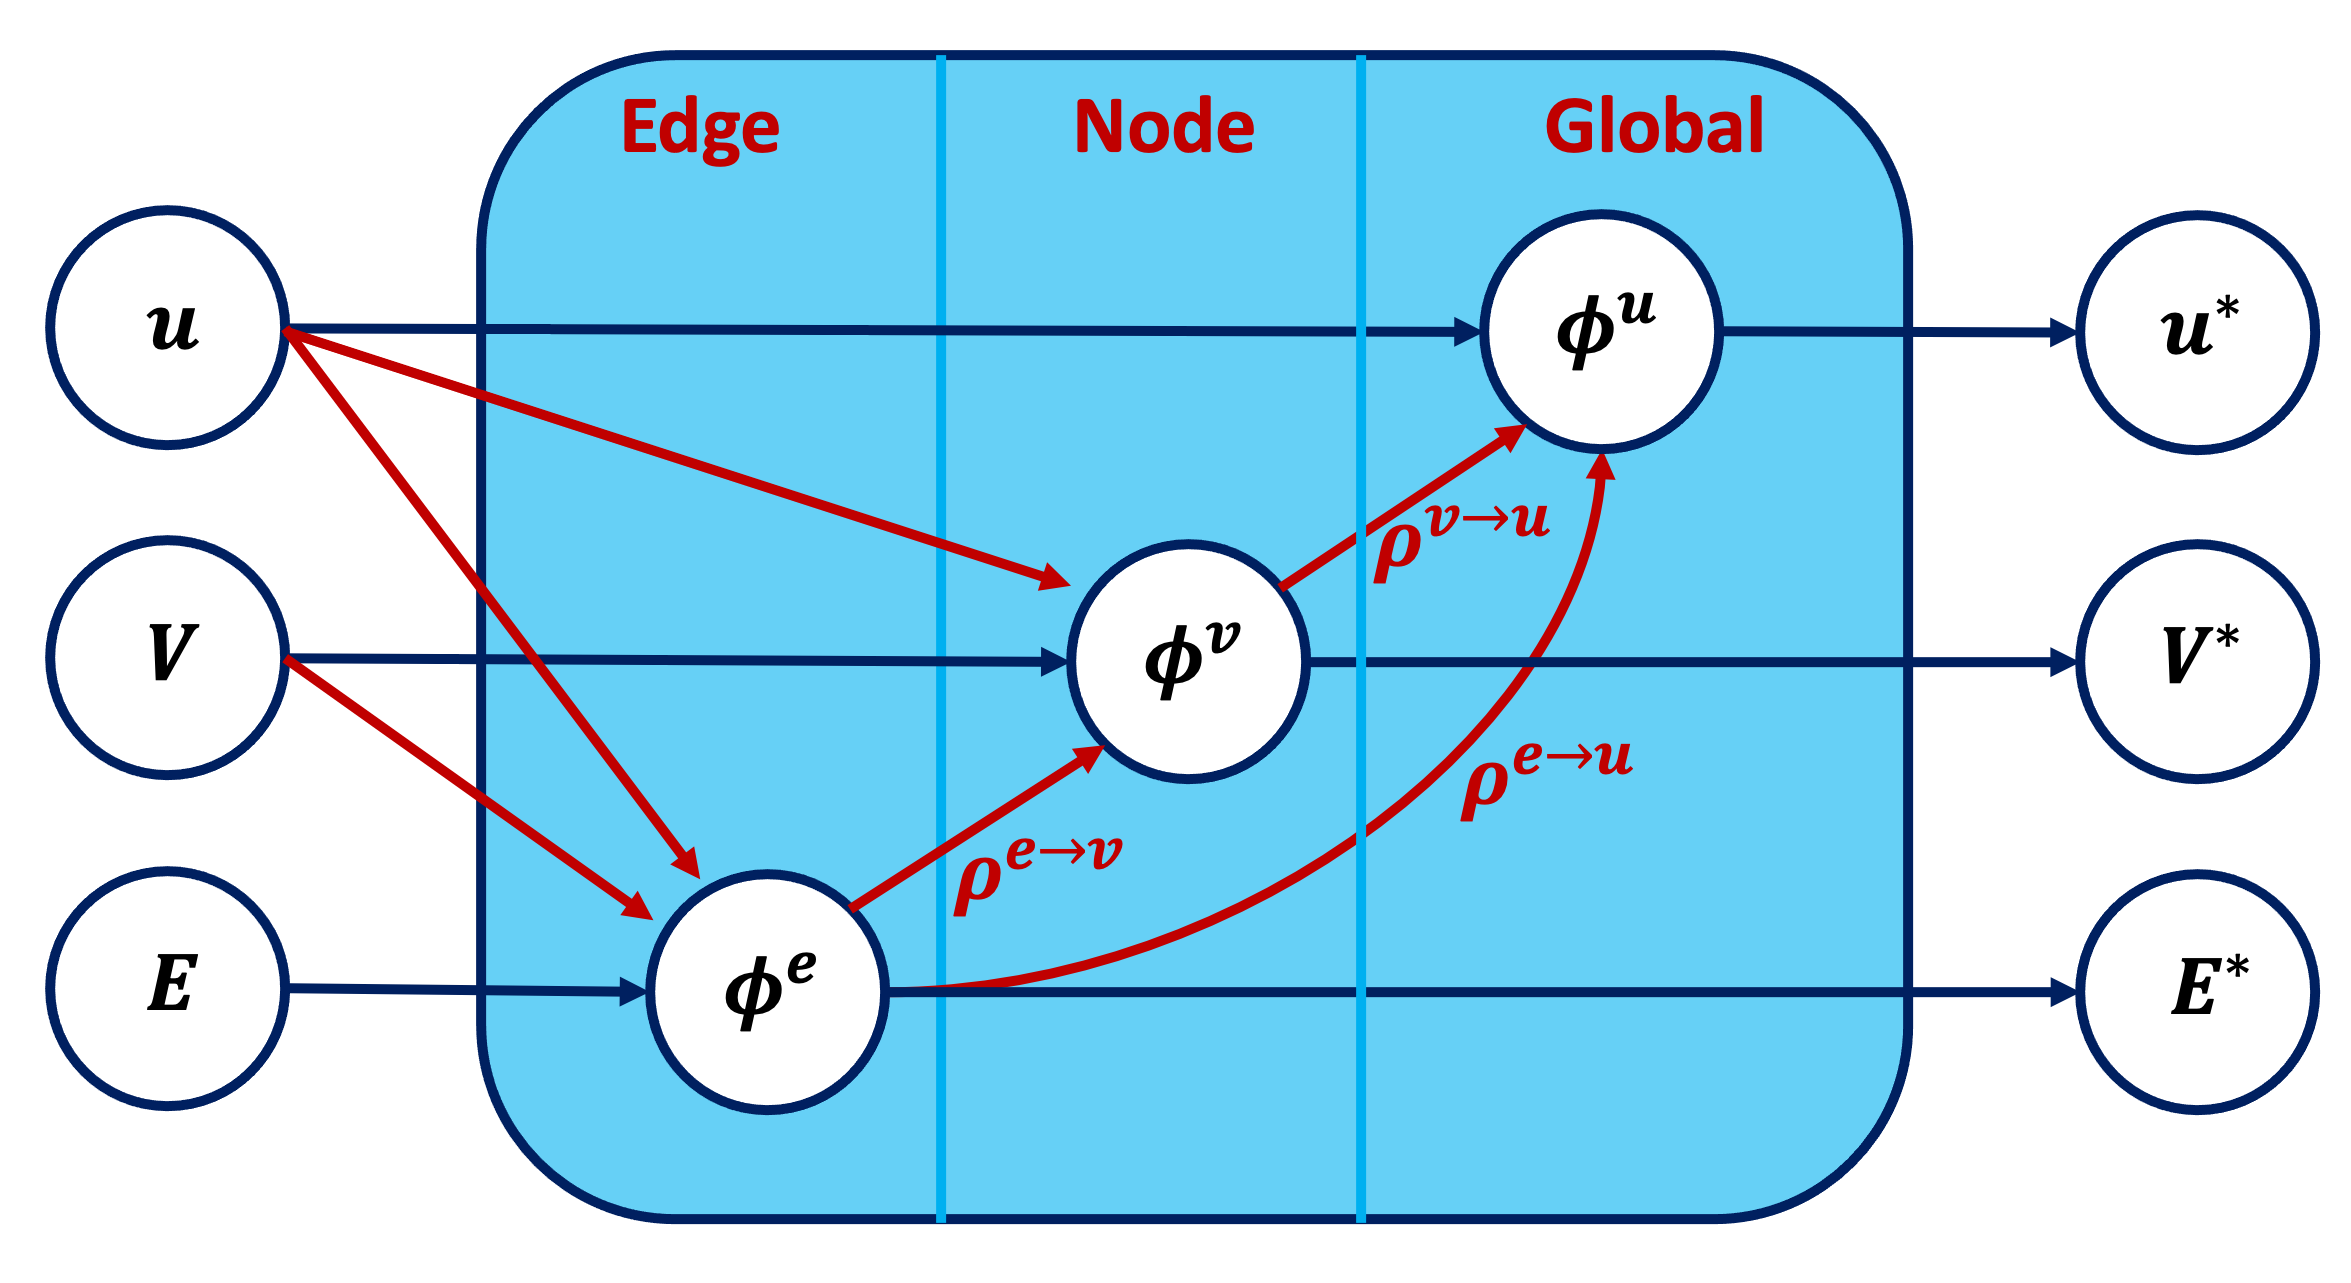
\includegraphics[scale=0.43]{Images/ML/fullGNN.png}
        \caption{Full \gls{gnn}.} 
        \label{fig:diverseGNNfull}
    \end{subfigure}
    \hfill
    \begin{subfigure}[b]{0.49\textwidth}
        \centering
        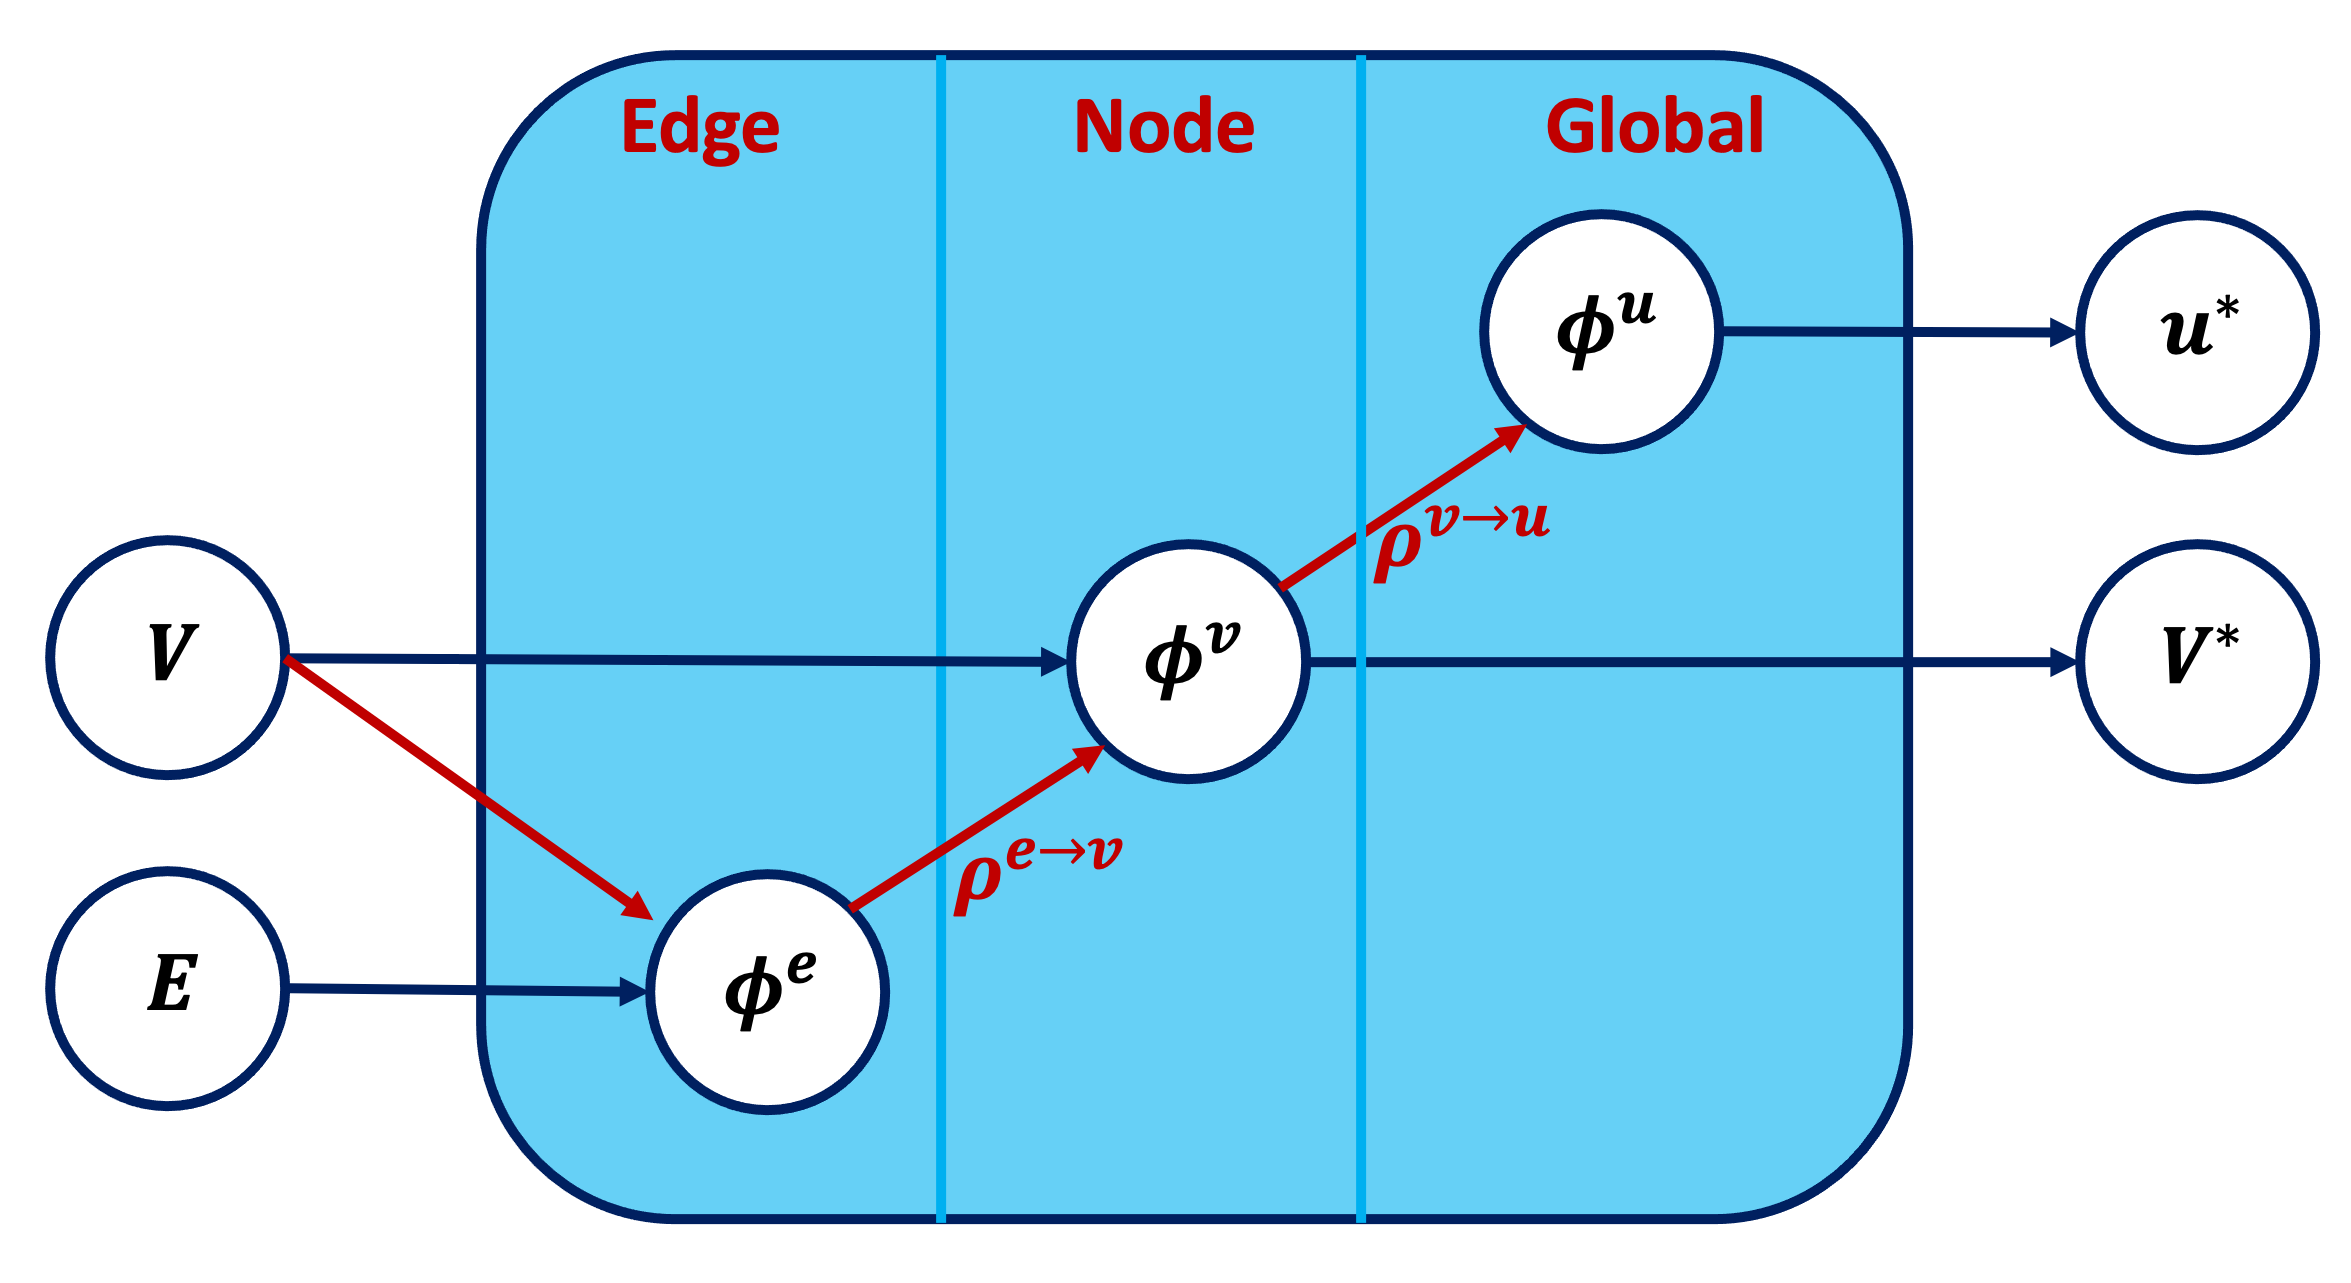
\includegraphics[scale=0.43]{Images/ML/messagepassingNN.png}
        \caption{Message-passing \gls{gnn}.} 
        \label{fig:pullsFTAGmp}
    \end{subfigure}
    \\  % newline
    \begin{subfigure}[b]{0.49\textwidth}
        \centering
        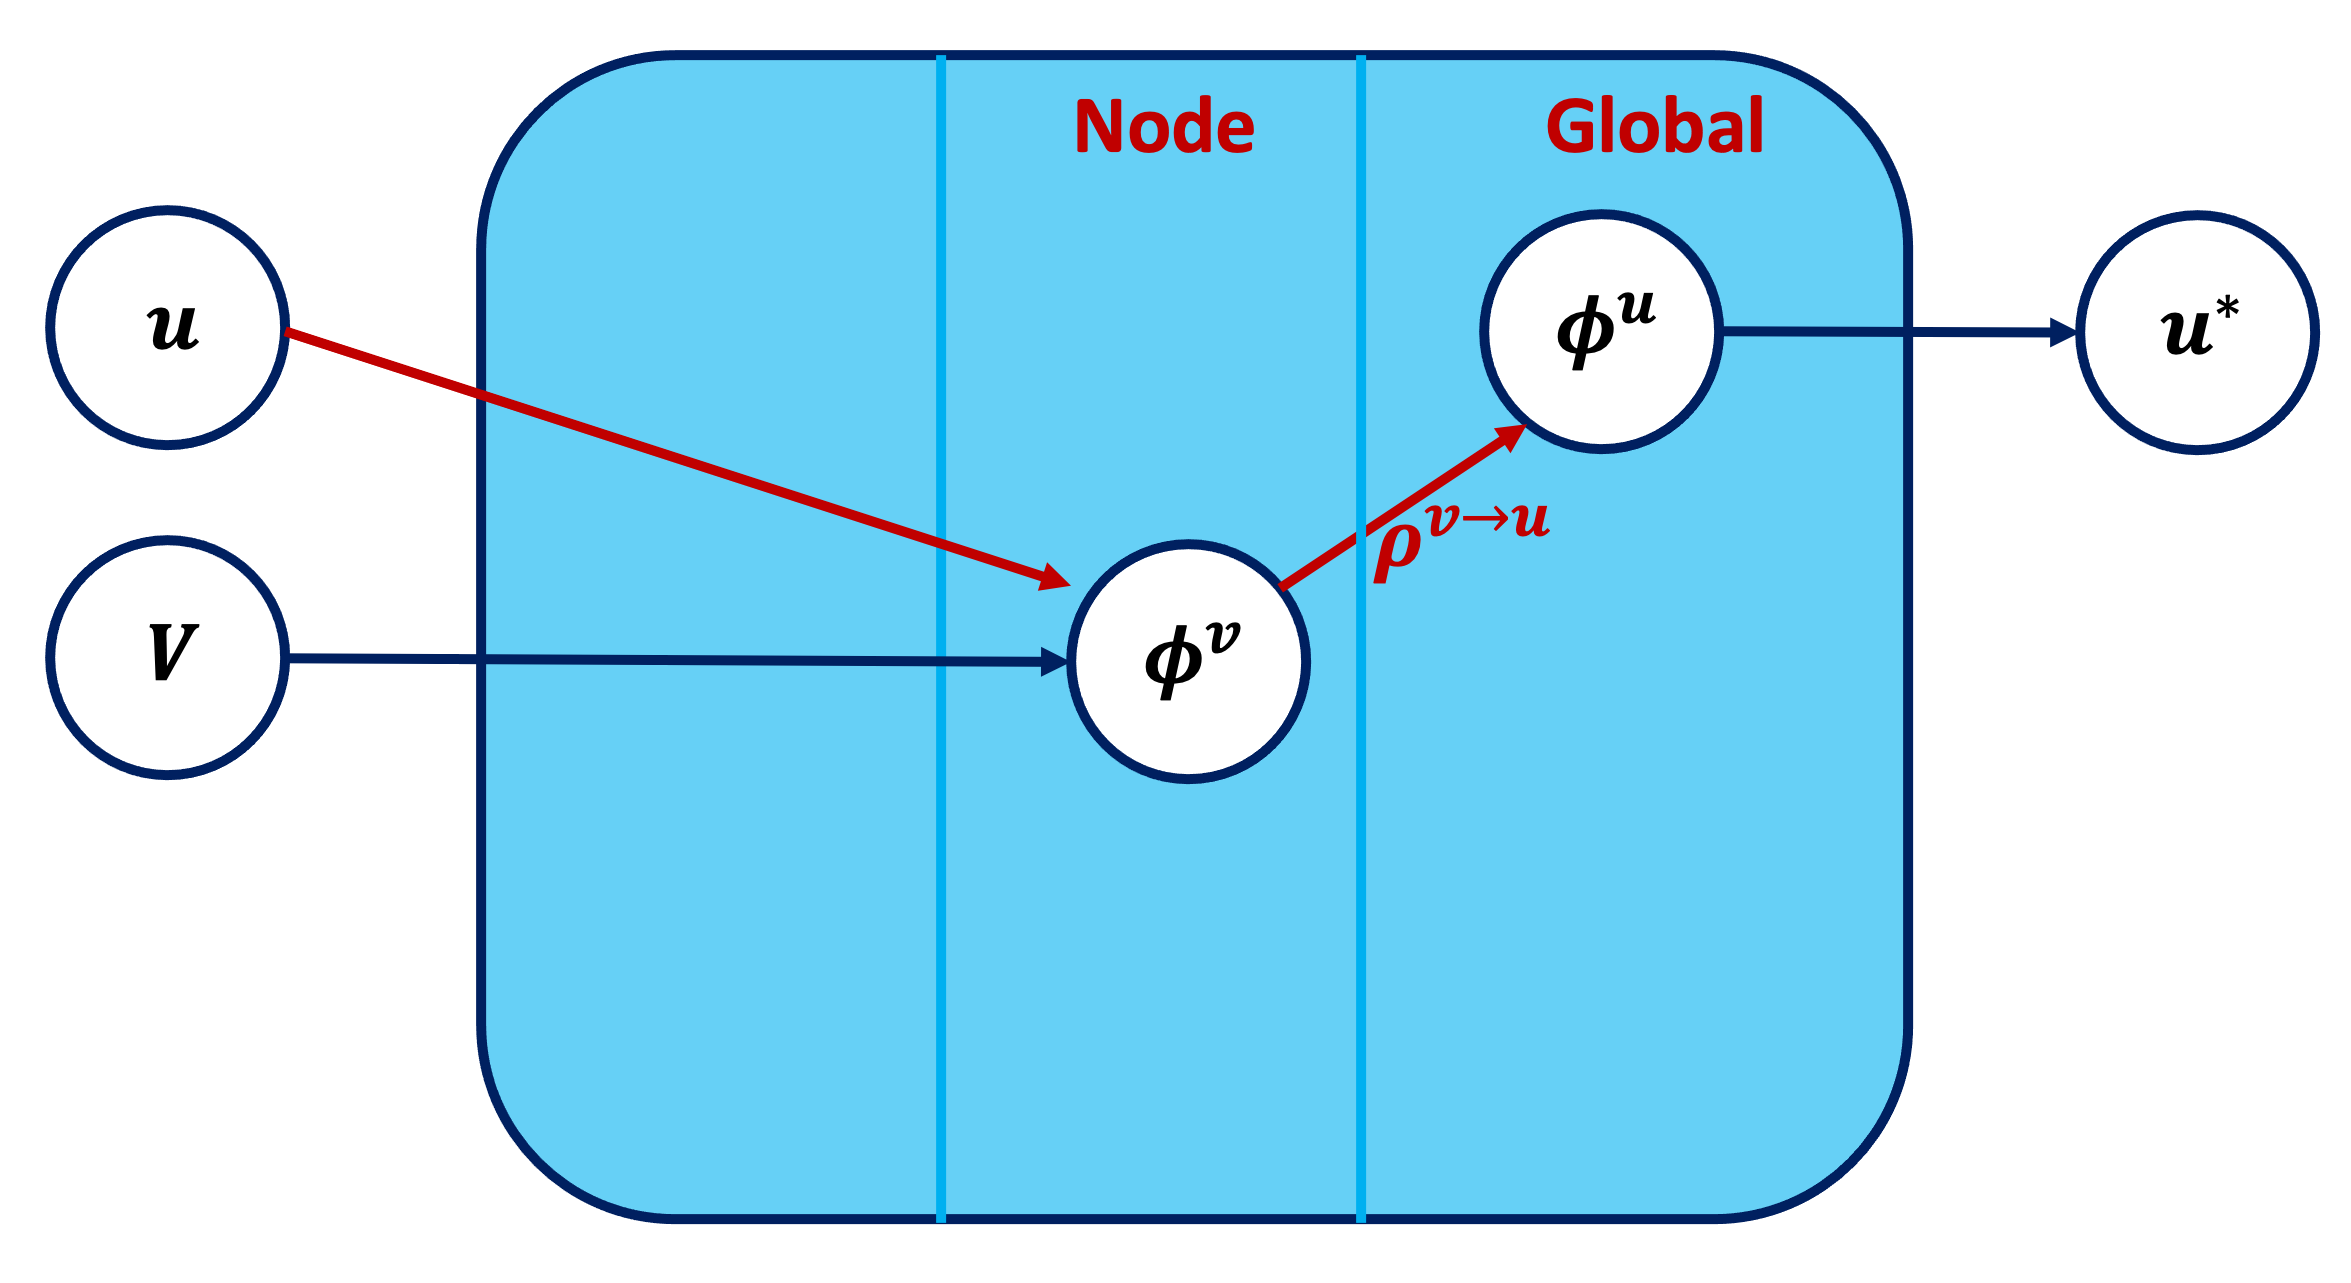
\includegraphics[scale=0.43]{Images/ML/deepSet.png}
        \caption{Deep Set.} 
        \label{fig:deepSetFig}
    \end{subfigure}
    \hfill
    \begin{subfigure}[b]{0.49\textwidth}
        \centering
        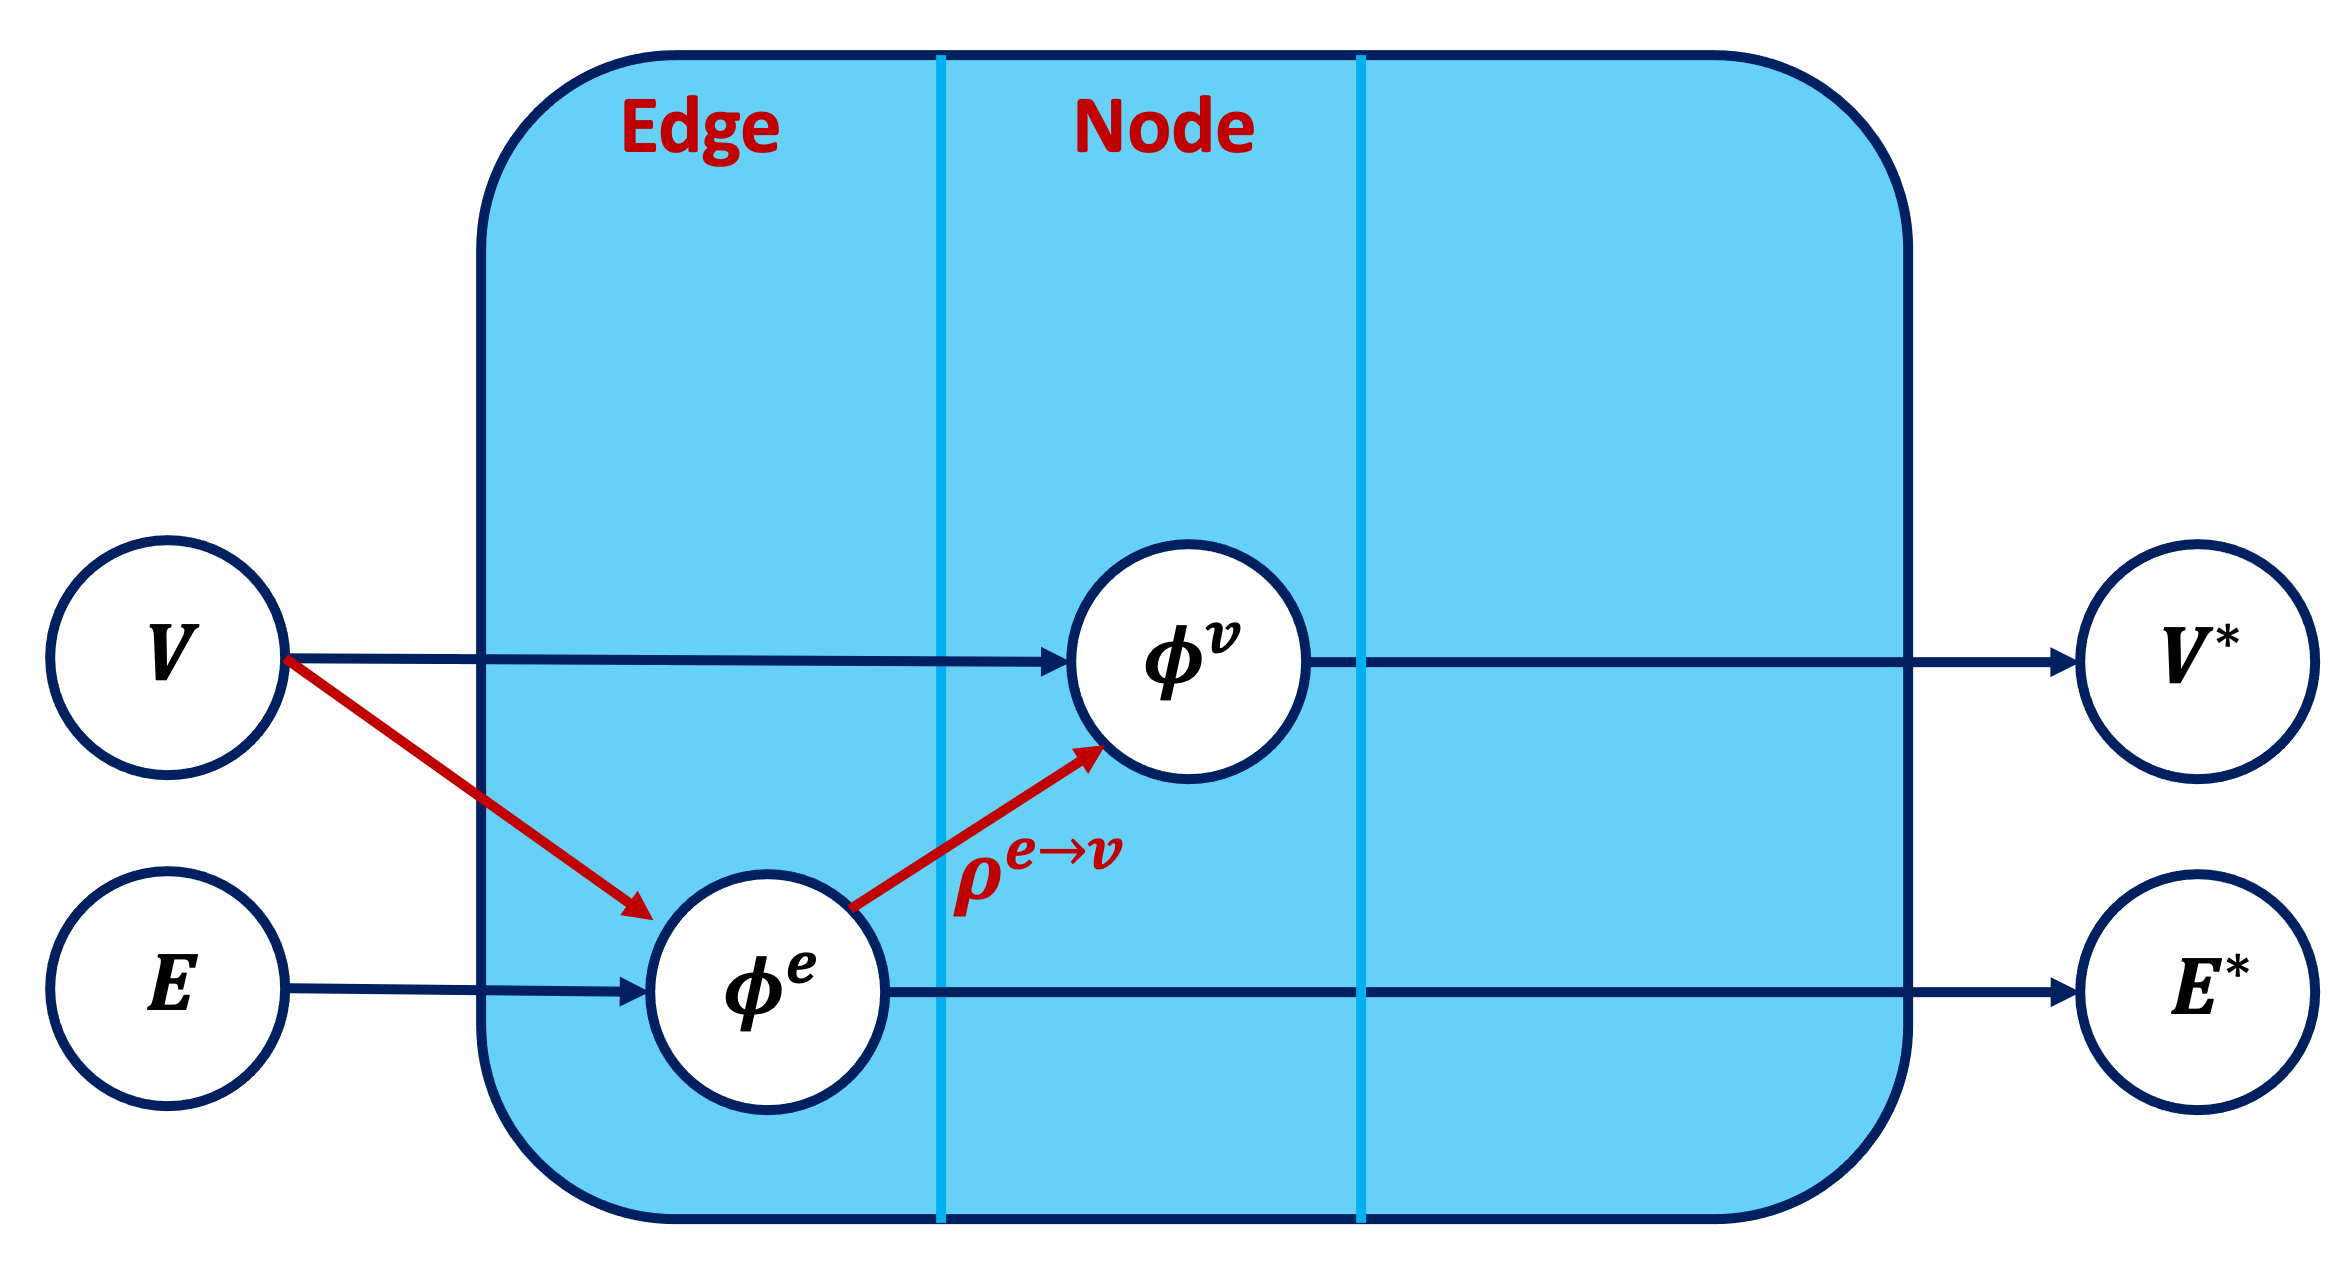
\includegraphics[scale=0.43]{Images/ML/nlnn.png}
        \caption{Non-local \gls{nn}.} 
        \label{fig:pullsFTAGnlnn}
    \end{subfigure}
    \caption{Different types of \gls{gnn} update rules, defining different \gls{gnn} architecture \cite{graphInductiveBias}.}
    \label{fig:diverseGNN}
\end{figure} 

A different approach introduced in \cite{nlnnPaper} defines the non-local neural network, unifying different types of \textit{attention}-based architecture. Attention is an essential feature of modern deep learning: it refers to how an element is given a weighted version of the inputs, with weights standing for the degree of attention to be given to each different part of the input. This concept is not restricted to \gls{gnn} but is easily encapsulated in this formalism. As will be shown in the next section, the Transformer is a special case of this non-local \gls{nn} family. In this section only the \gls{gat} is introduced for the sake of conciseness \cite{velickovic2018graph}. \gls{gat} introduces the attention mechanism by having a learnable weighting of the neighbour of the node being updated. When updating node $v_i$, a score is computed for each of the connected neigbour of $v_i$ by a \gls{nn} mapping: \[e(v_i, v_j) = \phi(v_i, v_j) = a^T \text{ leakyReLU}([W v_i, Wv_j]),\] where leakyReLU is the modification of the \gls{relu} with negative leakage, the nodes $v_i, v_j \in \mathbb{R}^d$ with $j$ connected to $i$, and the operation implements an embedding of the two nodes to a dimension $d'$ with two learnable parameters: $a \in \mathbb{R}^{2d'}$ and $W \in \mathbb{R}^{d' \times d}$. The operation $[,]$ stands for concatenation of the elements. These scores are then combined for each node $i$ over its neighbours $\{j\}$ to give attention scores $\alpha_{ij}$: \[ \alpha_{ij} = \text{softmax}_j (e(v_i, v_j)) = \frac{\exp(e(v_i, v_j))}{\sum_{j' \in \text{neighours of i}}e(v_i, v_{j'})}.\] The final step is to leverage these attention weights when updating each node $v_i$: \[v^*_i = \sigma\left(\sum_{j} \alpha_{ij} . W^v v_j \right),\] where the sum over $j$ is taken over neighbouring nodes of $i$, $\sigma$ is any activation function and $W^v$ is another matrix of learnable parameters.\\

\paragraph{Pros:}
\begin{itemize}
    \item \textit{Modeling Graph Structure:} \gls{gnn}s naturally handle graph-structured data, making them well-suited for tasks involving relationships between entities.
    \item \textit{Transferability:} Pre-trained \gls{gnn} models on one graph can be fine-tuned for related tasks on another graph.
    \item \textit{State-of-the-Art Performance:} \gls{gnn}s have achieved state-of-the-art results in various graph-related tasks, including node classification and link prediction.
\end{itemize}

\paragraph{Cons:}
\begin{itemize}
    \item \textit{Computational Complexity:} Training \gls{gnn}s can be computationally expensive, particularly for large graphs.
    \item \textit{Limited Global Context:} Some \gls{gnn} architectures may struggle to capture long-range dependencies in graphs, limiting their ability to consider global context.
    \item \textit{Interpretability:} Similar to other deep learning models, \gls{gnn} lack interpretability, making it challenging to understand the learned representations.
\end{itemize}

\subsection{The rise of the Transformers}\label{sec:transformer}

The Transformer architecture, introduced in 2017 \cite{NIPS_transformerPaper}, has become a foundational design for \gls{nlp} tasks. It has significantly impacted the field, enabling the development of state-of-the-art models such as BERT \cite{devlin-etal-2019-bert} and GPT \cite{radford2018improving}. More recentely, the transformer is also spearheading a revolution in computer vision tasks thanks to the generalisation of the architecture into the Vision Transformer (ViT) \cite{vitPaper}.

The Transformer architecture is based on the mechanism of self-attention introduced in the last section on graphs. As mentionned in section \ref{sec:RNN} on \gls{rnn}, it moves away from sequential processing and adopts a fully parallelised approach, allowing for efficient computation on dedicated hardware. The key components of the Transformer are the self-attention mechanism and position-wise feedforward networks. Self-attention allows the model to weigh the importance of different words or tokens in a sequence when assessing a specific token. This mechanism enables the model to capture long-range dependencies in the input data without the added complexity of \gls{lstm} or \gls{gru}. Strictly speaking, the input of a Transformer is a sequence that has no strict order. For \gls{nlp}, the important ordering of the sequence is built in the model using position-wise embedding. This lets the network decypher the index of the token in the input sequence and leverage this information for its tasks. For the computer vision case, the Vision Transformer first splits the input image $x$ into patches of fixed size, flattens them into a vector and maps them with a learnable positional embedding before processing them as a regular Transformer would.

\begin{figure}[h!]
    \center
    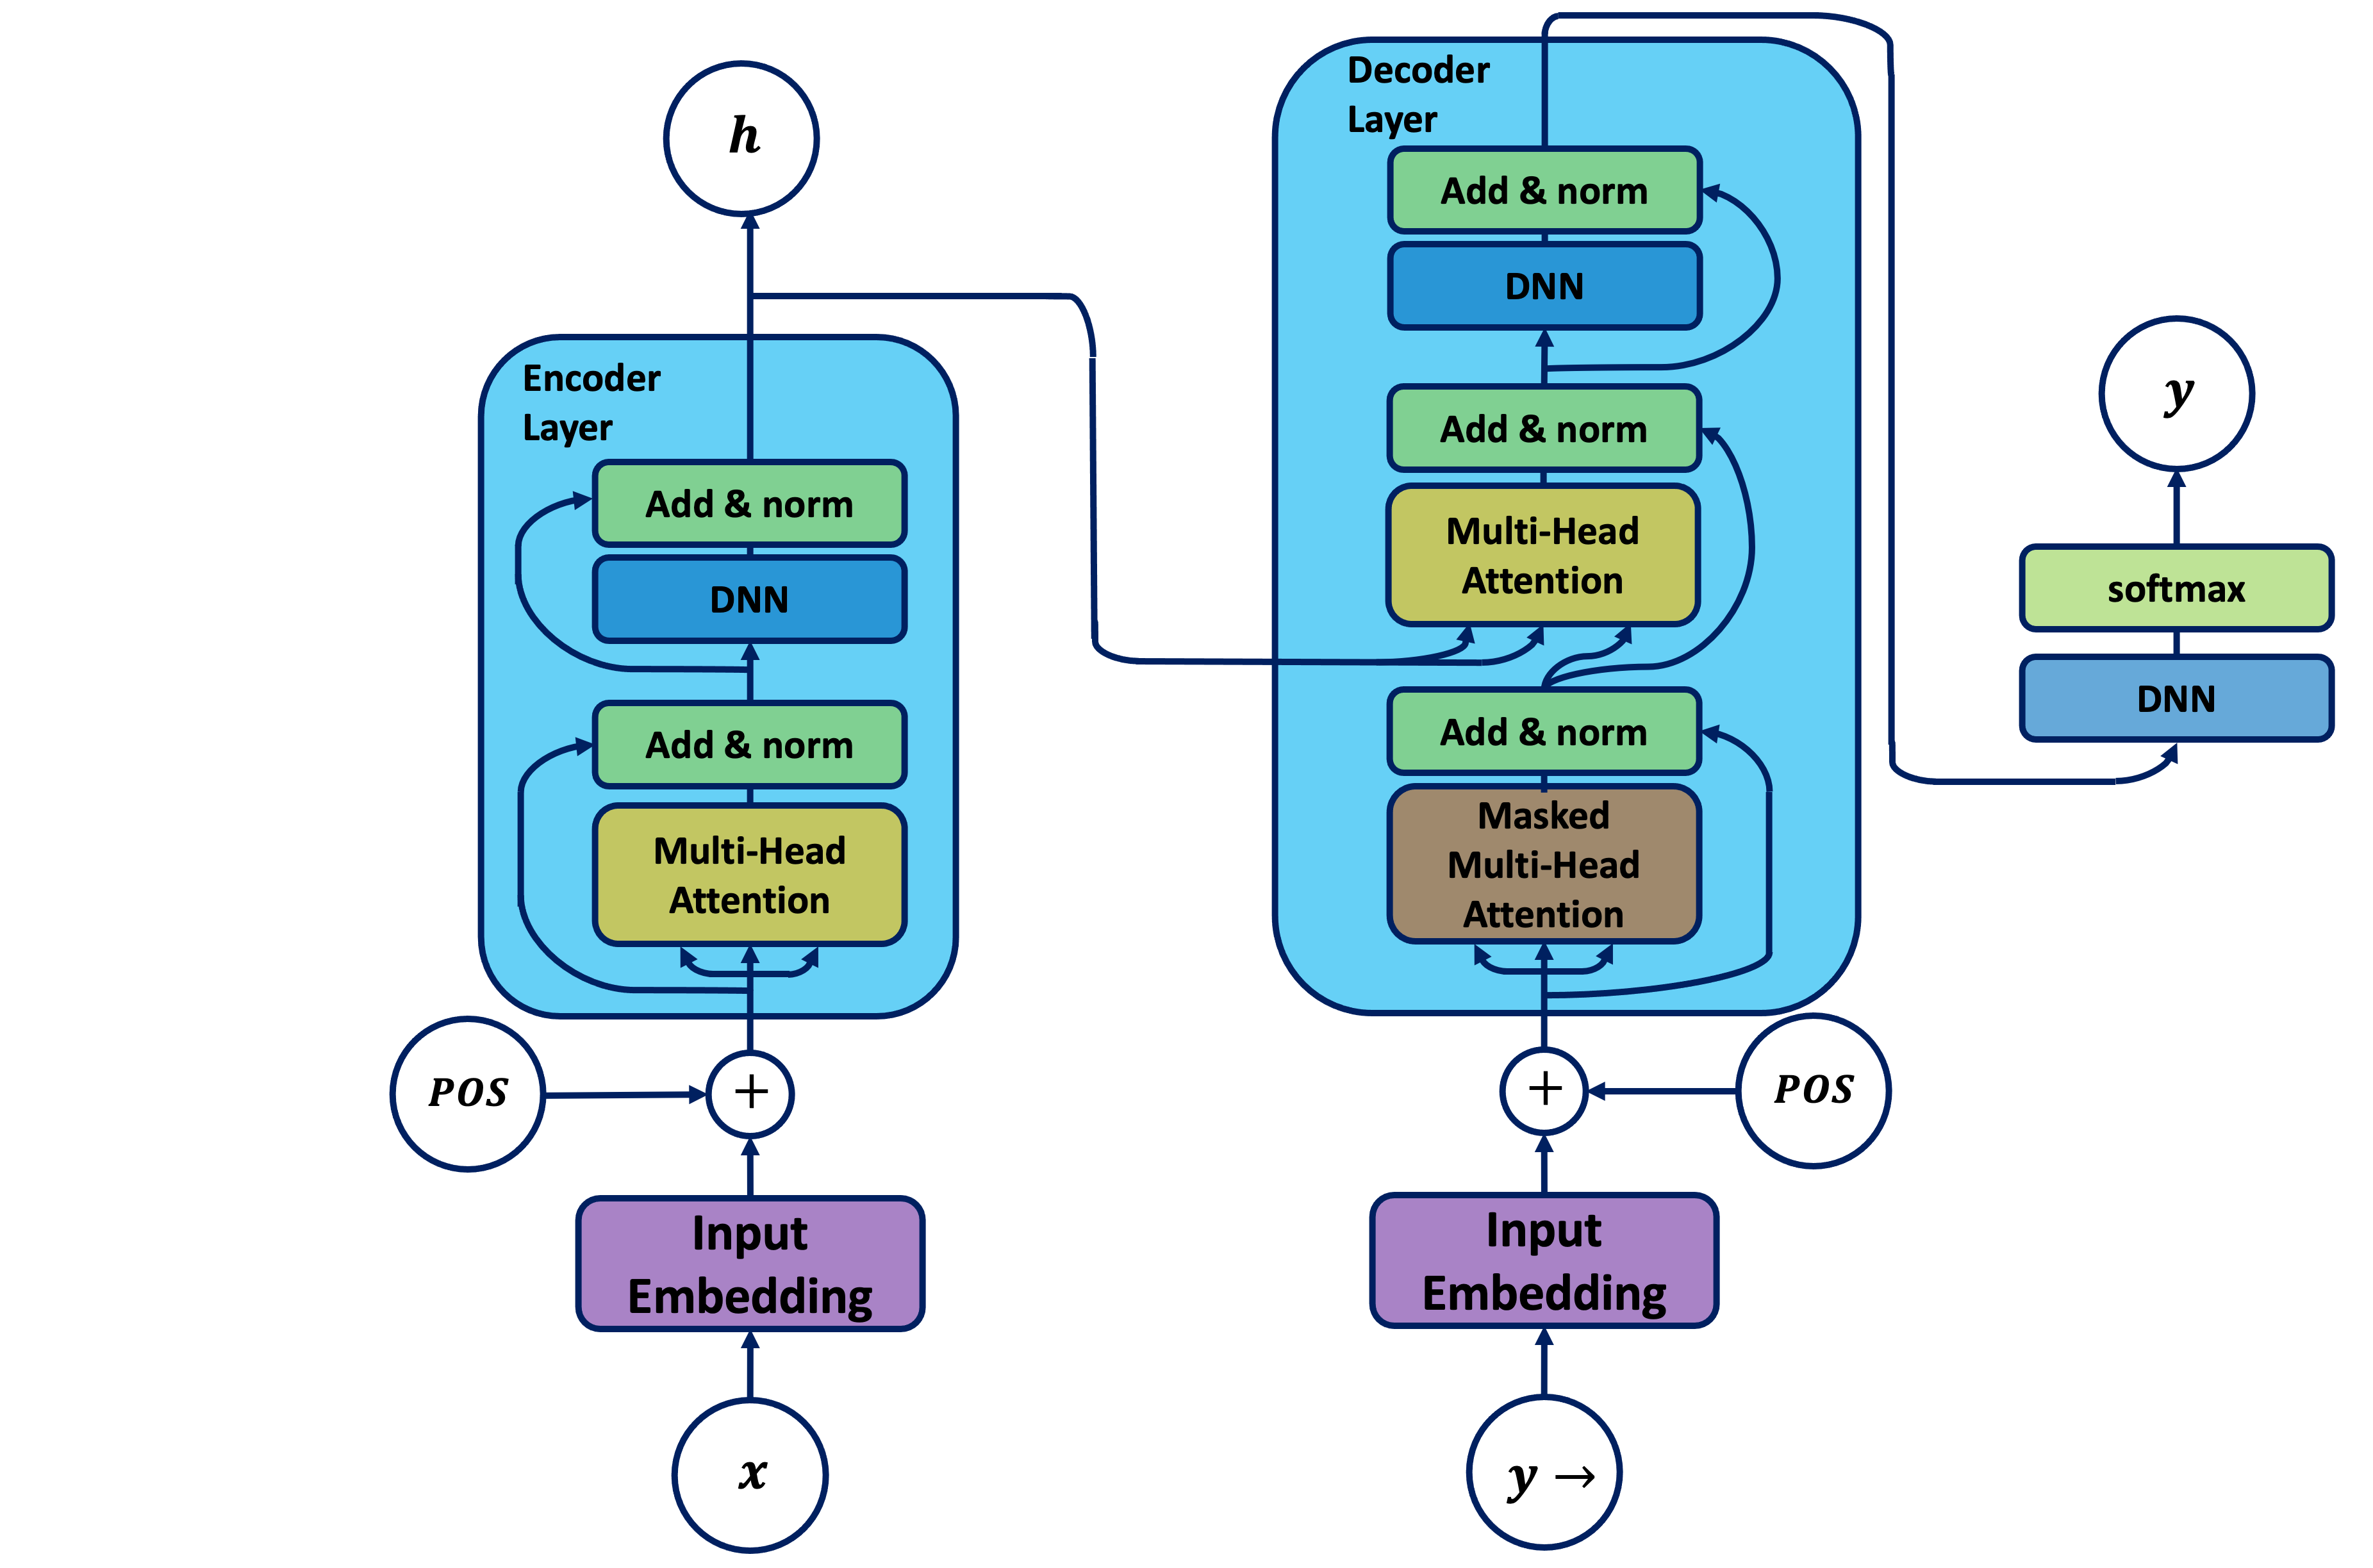
\includegraphics[scale=0.5]{Images/ML/transformer.png}
    \caption{The full transformer architecture, combining an encoder and a decoder each made of an arbitrary number of layers. The input $x$ is first embedded with a dedicated mapping which can, when order matters, be supplemented with positional embedding. The encoder generates an internal representation $h$ that is passed to the decoder. This component, depicted on the right, produces the next output using the internal representation $y$ and the output shifted to the right - to force output token to only access prior information. } 
    \label{fig:tranfoArchi}
\end{figure}

As presented in Figure \ref{fig:tranfoArchi}, the general Transformer architecture consists of an encoder and a decoder, the main feature of auto-encoder models. The decoder works in an autoregressive way, combining the current outputs $y_{t<T}$ with an internal representation $h$ built by the encoder to generate the next output tokens $y_{T}$. Both the encoder and the decoder are composed of multiple layers, each containing a multi-head self-attention mechanism and position-wise feedforward networks (\gls{dnn}). The decoder is further endowed with a masked attention layer, for the output to compute self-attention with information accessible prior to the token's position. The attention mechanism allows the model to focus on different parts of the input sequence, while the feedforward networks provide additional non-linear transformations. Residual connexions are added to let the gradients propagate efficiently in depth and layer normalisation is used after each block to avoid vanishing or exploding gradients and improve training speed \cite{ba2016layer}. This type of normalisation scales each activation (each neuron) by substracting the empirical mean and dividing by the standard deviation per datapoint. \\
The attention mechanism maps the queries and a set of key-value pairs to an output as defined in Equation \ref{eq:scdotatt} and schematised in Figure \ref{fig:scaledDotAtt}, with query $Q \in \mathbb{R}^{d_k \times d_q}$, key $K \in \mathbb{R}^{d_k \times d_v}$, and value $V \in \mathbb{R}^{d_v}$ and the output is a vector $\mathbb{R}^{d_q \times d_v}$ assigned a vector of attention values to each value per query. This combines $d_q$ different queries of the $d_k$ keys mapping to $d_v$ values. Equation \ref{eq:scdotatt} implements for each query weighted sum of the values, based on a compatibilty function established by comparing the queries and keys:
\begin{equation}\label{eq:scdotatt}
    \text{Attention}(Q, K, V) = \text{softmax}\left( \frac{Q^T . K}{\sqrt{d_k}}\right) V,
\end{equation} 
where the scaling by $\sqrt{d_k}$ is implemented to reduce the magnitude of the dot product $Q^T K$ and avoid landing in regions of saturation of the following softmax, that is applied per row of the formed attention matrix. This scaled dot-product attention mechanism leverages the extensive research into numerical optimisation of matrix multiplications, making this operation less time and memory demanding than using a \gls{dnn} mapping to compute the attention - a technique referred to as \textit{additive attention} \cite{Bahdanau2014NeuralMT}. As shown in Figure \ref{fig:mulitheadAtt}, multi-head attention runs this dot-product attention in parallel for $h$ different heads, each head $h_i$ ($i = 1, ..., h$) implementing a separate learnable projection from the input $Q$, $K$, $V$ with linear transformations of respective weights $W_i^Q \in \mathbb{R}^{d \times d_k}$, $W_i^K \in \mathbb{R}^{d \times d_k}$, and $W_i^Q \in \mathbb{R}^{d \times d_v}$, where $N$ is the length of the sequence, $d$ is the model dimension and $h$ the number of heads: \[Q_i = Q W_i^Q,\] \[K_i = K W_i^K,\] \[V_i = V W_i^V,\] \[H_i = \text{Attention}(QW_i^Q, KW_i^K, VW_i^V).\] The multi-head module then concatenates the $h$ different heads $H_i$ outputs and applies another linear tranformation of parameters $W^O \in \mathbb{R}^{hd_v \times d}$: \[\text{Multi-Head Attention}(Q, K, V) = \left[H_1, ..., H_h\right]W^o .\] In multi-head attention, there are therefore 3 different learnable projections $W_i^Q$, $W_i^K$, and $W_i^V$ per head and a single global projection $W^O$ for the output of the cell. Self-attention is a special case in which the input of the cell is not a tuple $(Q, K, V)$ of distinctive vectors but a single input $x \in \mathbb{R}^{N \times d_v}$ that is mapped out to the tuple with the learnable projections: \[Q = xW_i^Q,\] \[K = xW_i^K,\] \[V = xW_i^V.\]
The self-attention operation is equivalent to graph attention on a fully connected graph with only node features. 


\begin{figure}[h!]
    \centering
    \begin{subfigure}[b]{0.49\textwidth}
        \centering
        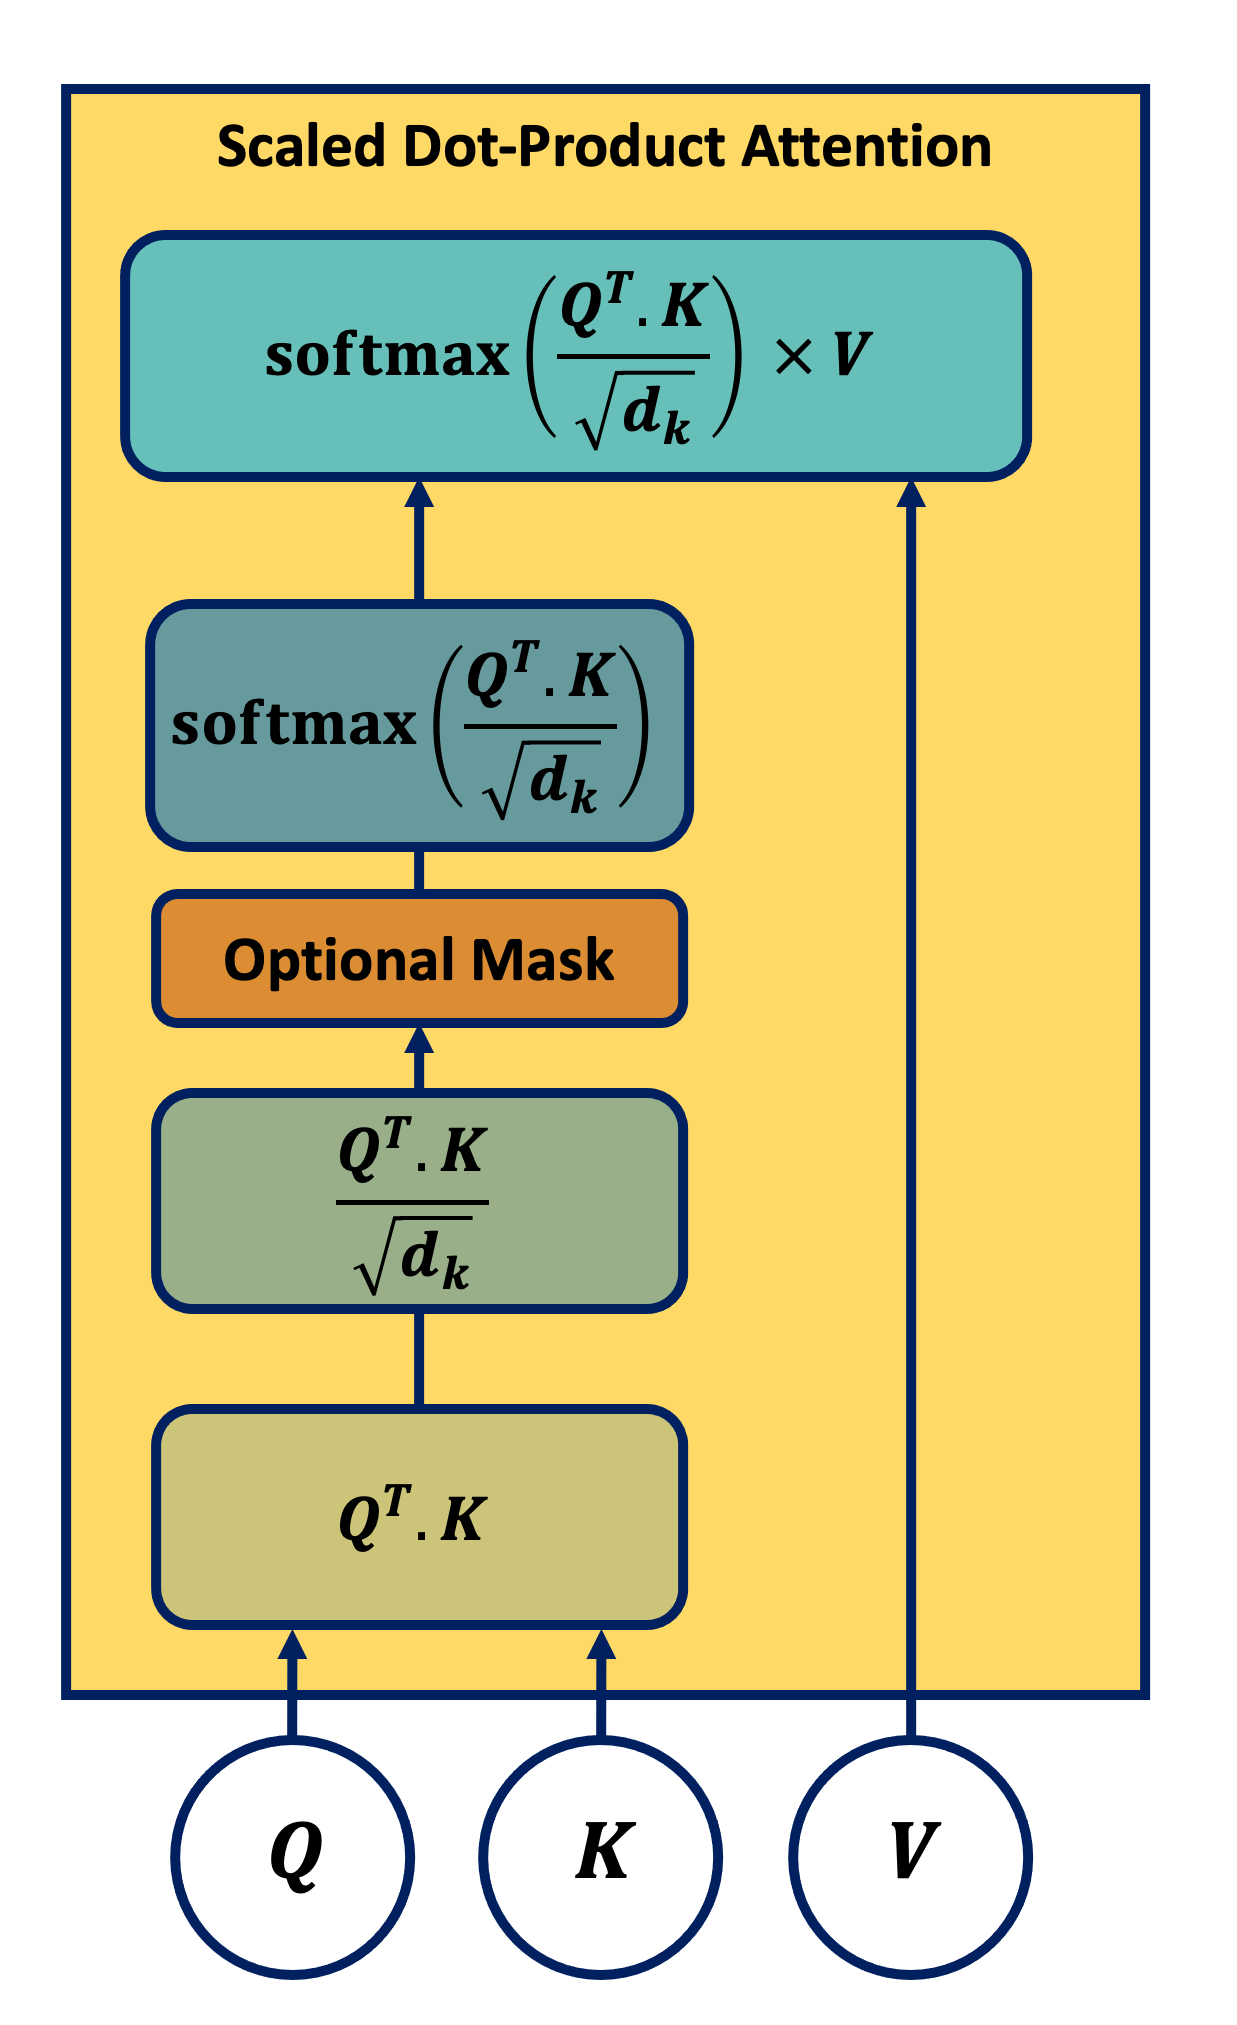
\includegraphics[scale=0.65]{Images/ML/scaledDotAtt.png}
        \caption{Scaled dot-product attention with optional masking.} 
        \label{fig:scaledDotAtt}
    \end{subfigure}
    \hfill
    \begin{subfigure}[b]{0.5\textwidth}
        \centering
        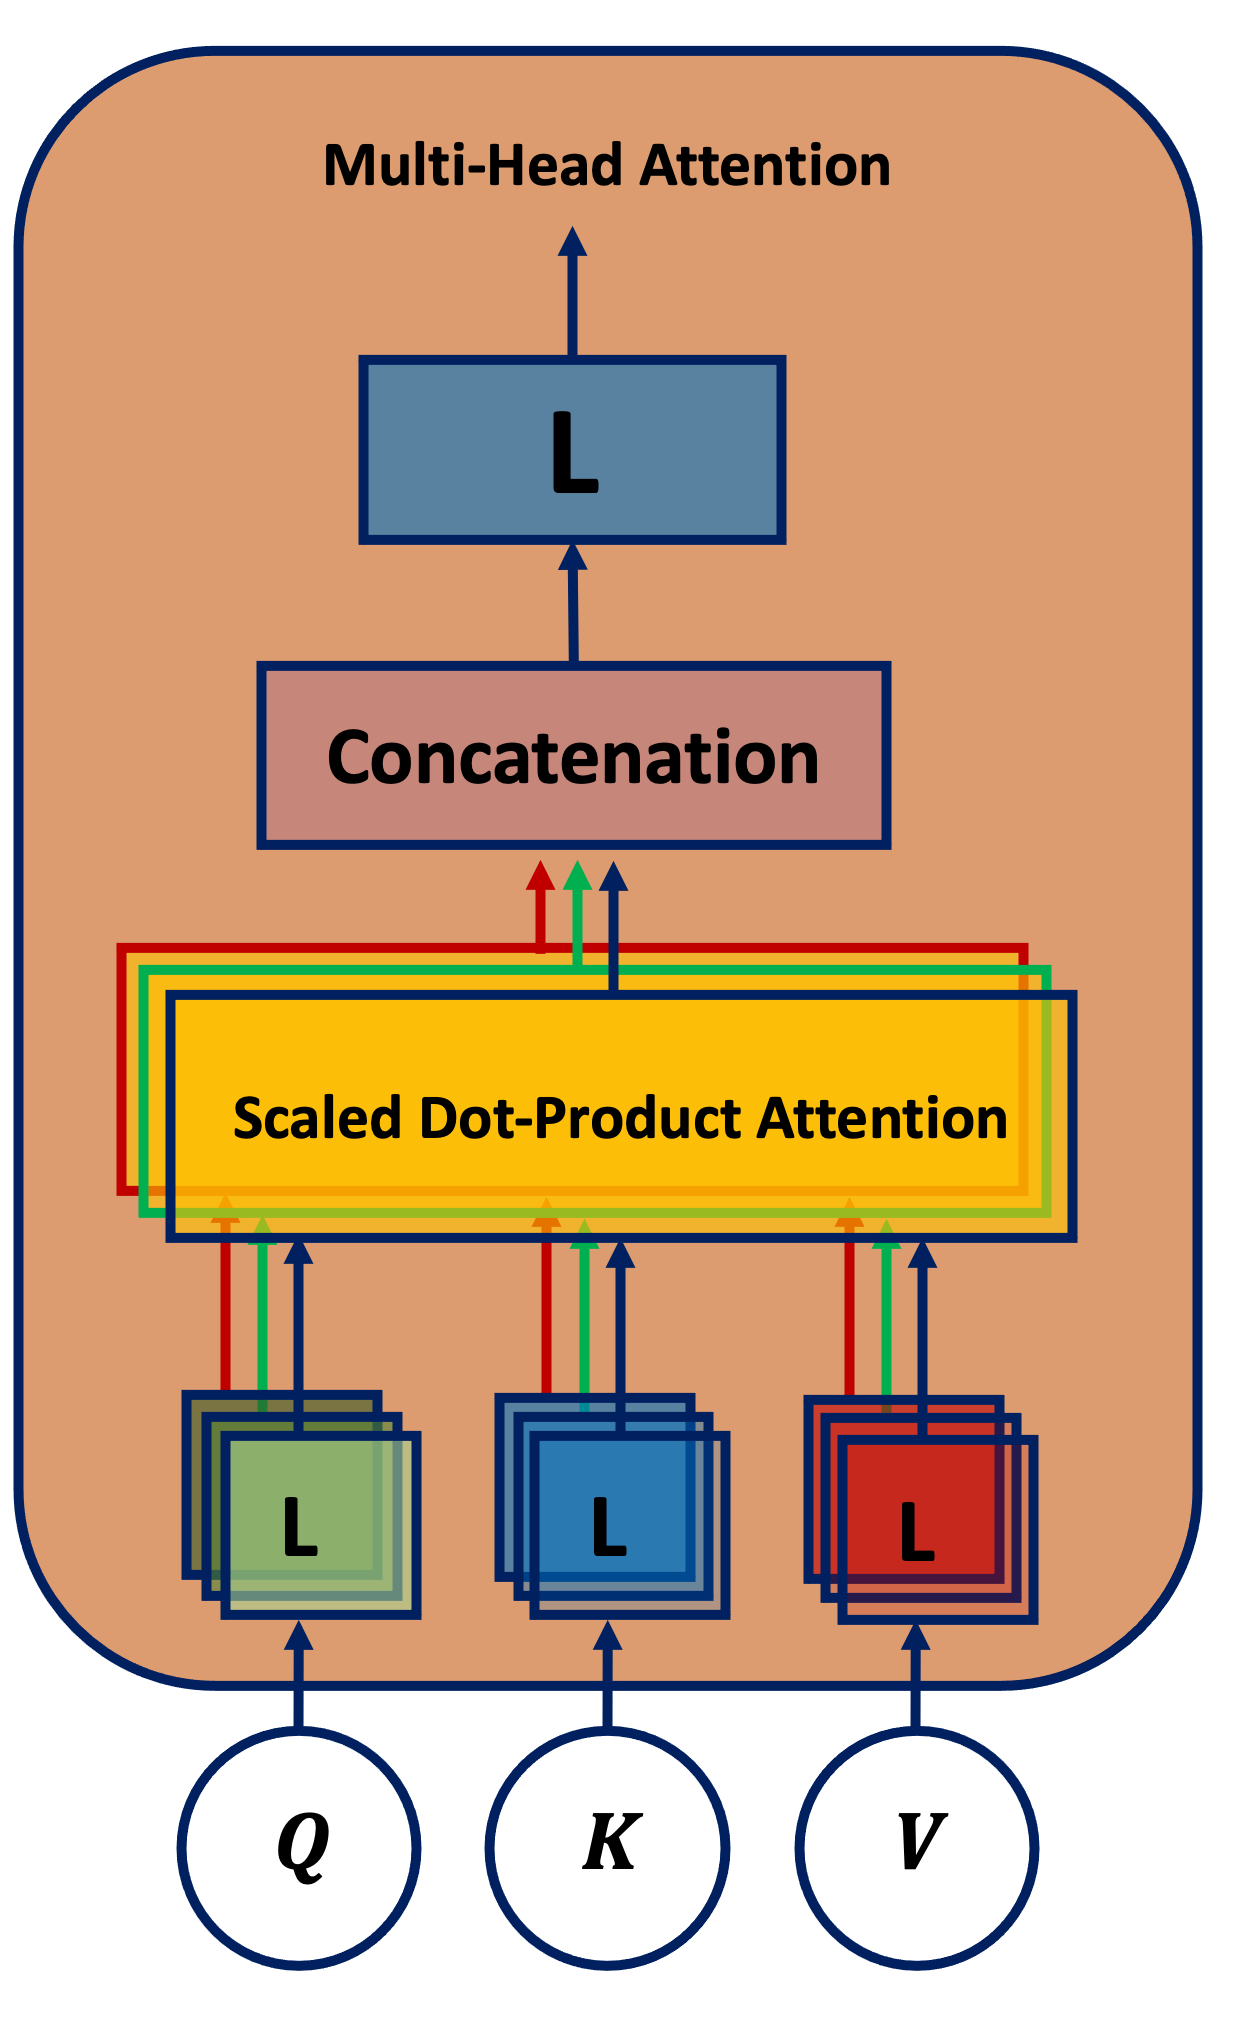
\includegraphics[scale=0.65]{Images/ML/multiHeadAtt.png}
        \caption{Multi-head attention module, where $L$ stands for a linear transformation of the input.} 
        \label{fig:mulitheadAtt}
    \end{subfigure}
    \caption{Multi-head attention mechanism in a transformer. The core operation is an optionally masked scalled dot-product of the queries $Q$, keys $K$, and values $V$. A head consists in three (optionally different) linear projection of the tuple $(Q, K, V)$, each leading to a separate scaled dot-product. The multi-head modules then concatenates all the different head results and finishes with another linear transformation.}
    \label{fig:transAtt}
\end{figure} 

\paragraph{Pros:}
\begin{itemize}
    \item \textit{Versatility:} The Transformer architecture has been successfully applied to various \gls{nlp} tasks - including machine translation, text summarization, and language modeling - and computer vision tasks.
    \item \textit{Parallelisation:} The architecture allows for efficient parallelisation of training, speeding up the learning process.
    \item \textit{Capturing Dependencies:} The self-attention mechanism enables the model to capture long-range dependencies in sequences.
    \item \textit{Stability:} per design Transformers benefit from regularisation effect due to residual connexions and normalisation layers. Models based on this structure can therefore scale to in complexity while resisting overtraining and with robust training conditions.
\end{itemize}

\paragraph{Cons:}
\begin{itemize}
    \item \textit{Computational Complexity:} Training large Transformer models can be computationally expensive, requiring powerful hardware.
    \item \textit{Interpretability:} The attention mechanism, while effective, can be challenging to interpret, making the model somewhat of a "black box."
    \item \textit{Data Dependency:} Transformer models may require large amounts of data for effective training, which may limit their application in domains with limited labelled data.
\end{itemize}

\section{Training and Optimising Deep Learning Models}
Training and optimising neural network models involve a combination of selecting appropriate architectures, fine-tuning hyperparameters - which cannot be learnt by backpropagation-, and employing acceleration techniques to improve efficiency and convergence. In this section, key aspects of the training process are explored, and acceleration techniques commonly used in practice are discussed.

\subsection{Training Algorithms}
When optimising the learnable parameters of a model, different training algorithms can be deployed to update the weights. All strategies are refinement on the base gradient descent rule of Equation \ref{eq:gradientdescent}, and each method has different advantages. The two main approaches are: 
\begin{itemize}
    \item \gls{sgd}: the update rule is the same as that of Equation \ref{eq:gradientdescent}, with the only difference being in how the gradient of the weights is computed. Instead of deriving it for the whole dataset (full-batch), the expectation over a random sub-batch is taken, hence the stochastic behaviour: \[ \nabla w = \frac{1}{b} \sum_{s=1}^b \nabla w_s,\] with $\nabla w_s$ being the gradients of the parameters computed for a single datapoint. A common observation is that for sub-batches - from now-on referred to as just \textit{batch} - of sufficient size, the stasticial estimator of the gradient based on the batch is unbiased. This greatly accelerates the time it takes to compute the gradient and naturally splits the loop over the dataset into different iterations called \textit{steps}, at which a batch is passed throught the network, a beneficial feature in the case of large datasets that would not fit in memory. This has also an effect on regularisation of the model, has each computed gradient on a batch has larger variance than a full-batch, making it harder for the model to overtrain. 
    \item Adam is an algorithm published in 2014 leveraging an adaptive moment estimation approach as well as batch processing \cite{adamPaper}. The moment in this sense is analoguous to the physical moment and encapsulates the dynamic of the optimisation as dervied by the gradient. The fundamental idea is that larger gradients indicate a steep slope that can be quickly traversed, so that any slowing down due to a changing curvature of the objective function landscape can be mitigated due to the inertia of the weights. This behaviour is implemented as an exponentially decaying moving average: the moment $m^t_w$ of weight $w$ at step $t$ is updated with a gradient forgetting factor $\beta_1 \in [0, 1[$ such that: \[ m_t \leftarrow \beta_1 m^{t-1}_w + (1 - \beta_1) \nabla_w \mathcal{L}^t,\] where the previous contribution are successively mutliplied by $\beta_1$ reducing the importance of earlier gradients progressively. Additionally, another element is taken into account in the gradient descent rule: the second moment $(\nabla_w \mathcal{L}^t)^2$. This tracks the magnitude of the gradient and, by multiplying the gradient update by a term inversely proportional to the second moment, accelerates the gradient updates in ``flatter'' regions of the objective landscape giving small gradient magnitudes with the term: \[ v_t \leftarrow \beta_2 v^{t-1}_w + (1 - \beta_2) (\nabla_w \mathcal{L}^t)^2,\] where a second moment forgetting factor $\beta_2 \in [0, 1[$ is introduced. To avoiding biasing the gradient update, both the momentum (first moment) and the second moment are corrected with \[\hat{m}^t_w \leftarrow \frac{m^t_w}{1 - \beta_1},\] and \[\hat{v}^t_w \leftarrow \frac{v^t_w}{1 - \beta_2}.\] The two contributions are then combined into a single gradient descent step following equation \ref{eq:adam}
    \begin{equation}\label{eq:adam}
        w^{t} \leftarrow w^{t-1} - lr \times \frac{\hat{m}^t_w}{\sqrt{\hat{v}^t_w} + \epsilon},
    \end{equation}
    where $\epsilon$ is added for numerical stability and is typically chosen to be a very small number to not bias the results.
\end{itemize}

A key hyperparameter in any gradient descent algorithm is the learning rate $lr$. There is no evident choice for this parameter and suitable values have to be derived on a case-by-case approach. A useful technique to let the training process converge to a good minimum of the loss function and avoid unsuitable local minima is to adapt a \textit{learning rate schedule}: the learning rate is modified throughout training to resolve different part of the loss function. Initially, having a relatively larger $lr$ allows the model to quickly update its weights in the direction of the minimum. If the rate is kept too high, the weights will not be able to approach the minimum and will overshoot or ``bounce' around the optimal set. In order to avoid this, the scheduler should reduce the learning rate so that smaller steps can be taken later in the training to approach the chosen optimum. At the beginning, the rate is typically not set to its maximum to start the gradient process in a valley of interest. An equivalent choice is to modify the batch size while keeping the $lr$ fixed \cite{smith2017decay}. This has also a regularising effect on the gradient: small batch sizes capture large variances and let the optimisation make drastic changes of orientation in the optimising function landscape, thereby avoid unsatisfactory local minima. Larger batch sizes stabilises the direction of descent, thereby offering a lower variance but potentially biased estimates towards a minimum. Combining these two characteristics at different epoch of the training is therefore an effective way to improve the training performance. Some methods, such as Adam, have other specific hyperparameters that should be optimised with the procedure described later in this chapter for hyperparameters.

\subsection{Regularisation}
Regularisation techniques are applied in the architecture and training procudure to prevent overfitting. Common methods include \textit{dropout}, which randomly drops connexions during training with Bernouilli probability distribution of parameter $p$, and L2 (L1) regularisations, which penalise large weights proportionaly to a penalisation parameter $\lambda$ times the sum of the squared (absolute value) of the weights. Both $p$ and $\lambda$ require careful optimisation as regularising the model can introduce bias and hit the overall performance. Additionally, batch normalisation is a technique that normalises the inputs of a layer over the batch, reducing internal covariate shifts. It helps stabilise and accelerate the training process. This is distinct from the layer normalisation used in the Transformer architecture of section \ref{sec:transformer} as the normalisation is carried over the batch samples rather than the activations. 

\subsection{Architecture \& Hyperparameters Optimisation}
There are several characteristics of the network that need to be optimised. Mainly: 
\begin{itemize}
    \item \textbf{Architecture Selection:} choosing the right architecture is crucial for the success of a \gls{nn}. Factors to consider include the complexity of the task, the nature of the data, and the desired trade-off between model complexity and interpretability. Limits in computing power should be factored in. Elements of the architecture include the type of \gls{ml} chosen (\gls{bdt}, \gls{dnn}, \gls{cnn}, \gls{rnn}, Transformer, ...), the choice of activation functions (\gls{relu}, tanh, ...), and the number of layers and nodes as well as connexions between the units.
    \item \textbf{Hyperparameter Tuning:} optimising hyperparameters - parameters that cannot be optimised with backpropagation of the gradients of the loss - is essential for achieving good model performance. Key hyperparameters include learning rate-related parameters, the batch size, and regularisation parameters.
\end{itemize}
The optimisation process for both hyperparameter tuning and architecture selection is expensive: it requires training and testing models with different combinations of hyperparameters or model architecture to evaluate their respective performance and uncover the best peforming options. Techniques such as grid search, random search, and Bayesian optimisation can be employed to efficiently explore the hyperparameter space. Architecture search is usually performed by trials and attempts, and the literature offers insights and guidance into what models might best perform in specific situations. 

\subsection{Acceleration Techniques}
Training an \gls{ml} model is often a computationally demanding tasks that can be carried out more effectively on specifically designed hardware and with some tricks in the process. 
\begin{itemize}
    \item \textbf{Parallel Dataloading:} loading data in parallel can significantly speed up the training process. Libraries like TensorFlow and PyTorch provide functionalities for efficient parallel dataloading. Instead of preparing a single batch, multiple batches can be loaded by different processing units in parallel to avoid this step becoming a bottleneck in performance. 
    \item \textbf{Early Stopping:} to prevent overfitting and save computation time, early stopping involves monitoring the model's performance on a validation set and halting training when performance ceases to improve.
    \item  \textbf{Hardware Accelerators:} specialised hardware accelerators can further accelerate training. The \gls{gpu} architecture is design to perform simple mathematical operation in parallel. This is precisely the needs of \gls{nn} optimisation, as each computational step consists in a matrix multiplication. Utilising \gls{gpu} for training and inference can give substantial speedups compared to \gls{cpu}-based computing. Other types of hardware optimised for \gls{dl} include the Tensor Processing Units (TPU) and the Neural Processing Units (NPU). 
    \item \textbf{Transfer Learning:} transfer learning leverages pre-trained models on large datasets and applies them to a new task. The idea is that there are some fundamental simularities between the new task and the task used to train the fondational model that will let this latter one start with useful information. Fine-tuning these models on specific tasks can significantly reduce the required training time and data compared to training a model from scratch. This approach is becoming increasingly fashionable, as larger \textit{foundational} models trained on multiple tasks with huge datasets can then be applied to a specific task, with the pre-trained weights either kept fixed or free to be modified to optimise the new task. New modules can also be added on top the foundational model to specialise it to a specific use-case. Such large foundational models are already available in \gls{nlp} (e.g., the Mistral 7B \cite{jiang2023mistral} - a 7 billion parameters Transformer capable of analysing English sentences and code) and computer vision (e.g., the Florence-2 model by Microsoft \cite{xiao2023florence2} - built on a Transformer with 0.5 billion parameters).
\end{itemize}
Training and optimizing deep learning models involve a combination of careful architectural choices, hyperparameter tuning, and the use of acceleration techniques. Selecting the most appropriate techniques is a task-specific challenge that will further depend on available resources and the desired trade-offs between training time and model performance as well as interpretability.


%\newpage
\chapter{\color{oxfordblue} Flavour Tagging}\label{chap-ftag}
\ChapFrame

\textit{
The focus of this chapter is on an essential task in the ATLAS experiment: identifying particles flying through the detector. This objective of assigning labels to reconstructed particles from measurements is referred to as tagging. An important family of particules to be tagged are quarks, and disentangling which specific flavour of the quarks should be assigned to an observed signal is called flavour tagging. Free quarks and gluons hadronise as per the rules of \gls{qcd}, forming large number of particles that can themselves further decay. Such a dynamic results in a many particles radiating within a clone centred around the inital flavoured particle, a structure referred to as a jet. Consequently, this chapter introduces method to tag jets, as labelled by the flavour of the initial parton. In particular, the different algortihms and methods relevant for this task developped during the during of the author's contribution to ATLAS are reviewed, with the first trainings of DIPS, DL1d, GN1, and GN2 described in details as well as early studies of the hyperparameter optimisation of GN2.
}

\section{Heavy-Flavour Jet Tagging}
A fundamental ingredient in any ATLAS analysis is the ability to correctly identify particles in the aftermath of a collision, from $\tau$-leptons, to $b$- and $c$-quarks, and gluons $g$. Having well-calibrated and optimally performing b- and c-tagging tools is of primary importance in studies of the Higgs boson couplings to $b$- and $c$-quarks. It is also critical for top $t$-quark measurements and searches for extensions of the \gls{sm}. As described by the theory of \glsfirst{qcd}, colour-charged objects, such as a $b$- or a $c$-quark, undergo hadronisation to form collections of colourless hadrons. These hadrons, mostly $B$ for $b$-quark and $D$ for $c$-quark, are quasi-stable and further decay in the volume of the detector. Such a succession of decays leaves a collection of particles within a cone oriented in the direction of the original parton, an easily recognisable pattern referred to as a \textit{jet}. From an analysis of the complicated structure of the jet, the flavour of the initially decaying particle can be reconstructed. The labelling scheme applied to jet consist in identifying the hadron associated to the jet: a $b$-jet must contain at least one $b$-hadron, a $c$-jet at least one $D$-hadron and no $b$-hadron, and if none of these hadrons are found the jet is said to be a light-jet, thereby grouping $u$-, $d$-, and $s$-quarks with gluons $g$. This is the task of \textit{flavour tagging}, and the tool to achieve this identification is called a \textit{tagger}. \\

\subsection{Decay Topology}
When a $b$-quark is produced, such as in the aftermath of a hard scatter due to a proton-proton collision, it quickly undergoes the process of hadronisation to neutralise its free colour-charge. This process leading free quarks and gluons to a final state of hadrons and leptons is intrinsically non-perturbative and can only be described with phenomenological models of framgentation \cite{Webber:419784}. The family of $b$-hadrons is composed of different ensemble of a bottom quark $b$ with one or more light quarks. These include the $B$-mesons, mainly $B^0=d\bar{b}$, $B^-=\bar{u}b$, $B^+=u\bar{b}$, and the strange and charmed $B$-mesons, and baryons, such as the $\Lambda_b^0=udb$ \cite{ATL-PHYS-PUB-2014-008}. For $b$-quarks, the hadronisation process is hard and most ($\sim$ 70-80\%) of the quark momentum is passed to the $b$-hadron \cite{Webber:419784}. Tagging $b$-jets benefits from a particularly advantageous configuration: the $b$ is the lightest element of the third generation of quarks and must decay through a flavour-changing process through the weak interaction. Because of the relatively small \gls{sm} value of the $V_{bc}$ \gls{ckm} matrix element, decay processes involving a transition $b \rightarrow c$ are suppressed, giving $b$-hadrons a characteristically long proper lifetime $\tau_B \approx 1.5$ ps corresponding to a proper decay length $c\tau_{B} \sim 450$ $\mu$m \cite{Tanabashi:2018oca}. In the laboratory frame and considering the boost of the $b$-hadron given by a Lorentz $\gamma$ factor ($\gamma > 1$) and $\beta = v/c \approx 1$ in the high energy limit, the distance travelled is given by \[d = \gamma \beta c \tau_B \approx \gamma c \tau_B.\] In the high-energy limit, $\gamma \approx E_B / m_B$, where the mass of $B$-hadrons is in the range 5-6 GeV. Consequently, a 50 GeV $b$-hadron decays at a distance of $d \approx 4.5$ mm from the primary vertex which can be resolved. This distance travelled, also called the $b$-hadron radius $L_{xy}$, further increases with jet $p_T$ and at transverse momentum above $\sim$500 GeV even overpasses the first detector layer of the \gls{ibl}, located at a distance of roughly 33 mm from the centre of ATLAS as shown in Figure \ref{fig:bhaddecay}. The location of the $b$-hadron decay can often be reconstructed by the ATLAS detector, and the reconstructed point of decay is called \gls{sv} \cite{Aad:2019aic}. Some important variables describing the decay of $b$-hadrons are the \glspl{ip} $d_0$ and $z_0$ of the charged particles emanating from the \gls{sv}. As shown in Figure \ref{fig:bjet}, $d_0$ and $z_0$ are the transversal and longitudinal distances from the primary vertex to the perigee\footnote{The point of closest approach.} of the track associated with the charged particle. For a $b$-jet, the \glspl{ip} can be large thanks to the long lifetime of the associated hadron. On average, a $b$-hadron decays weakly to four or five charged stable particles \cite{ATL-PHYS-PUB-2014-008}. Another characteristic of $b$-jets is the likely presence of leptons in the jet cone, as 40\% of the decays of $b$ and $c$-hadrons are semi-leptonic and include either an $e$ or a $\mu$ \cite{Tanabashi:2018oca}. \\

\begin{figure}[h!]
\center
\begin{subfigure}[b]{0.48\textwidth}
  \centering
  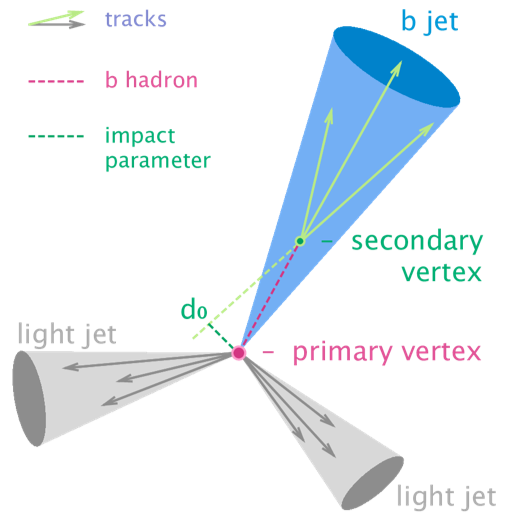
\includegraphics[width=0.9\textwidth]{Images/bjet}
  \caption{Representation of a $b$-jet \cite{bjetimage}.}
  \label{fig:bjet}
\end{subfigure}
\begin{subfigure}[b]{0.49\textwidth}
  \centering
  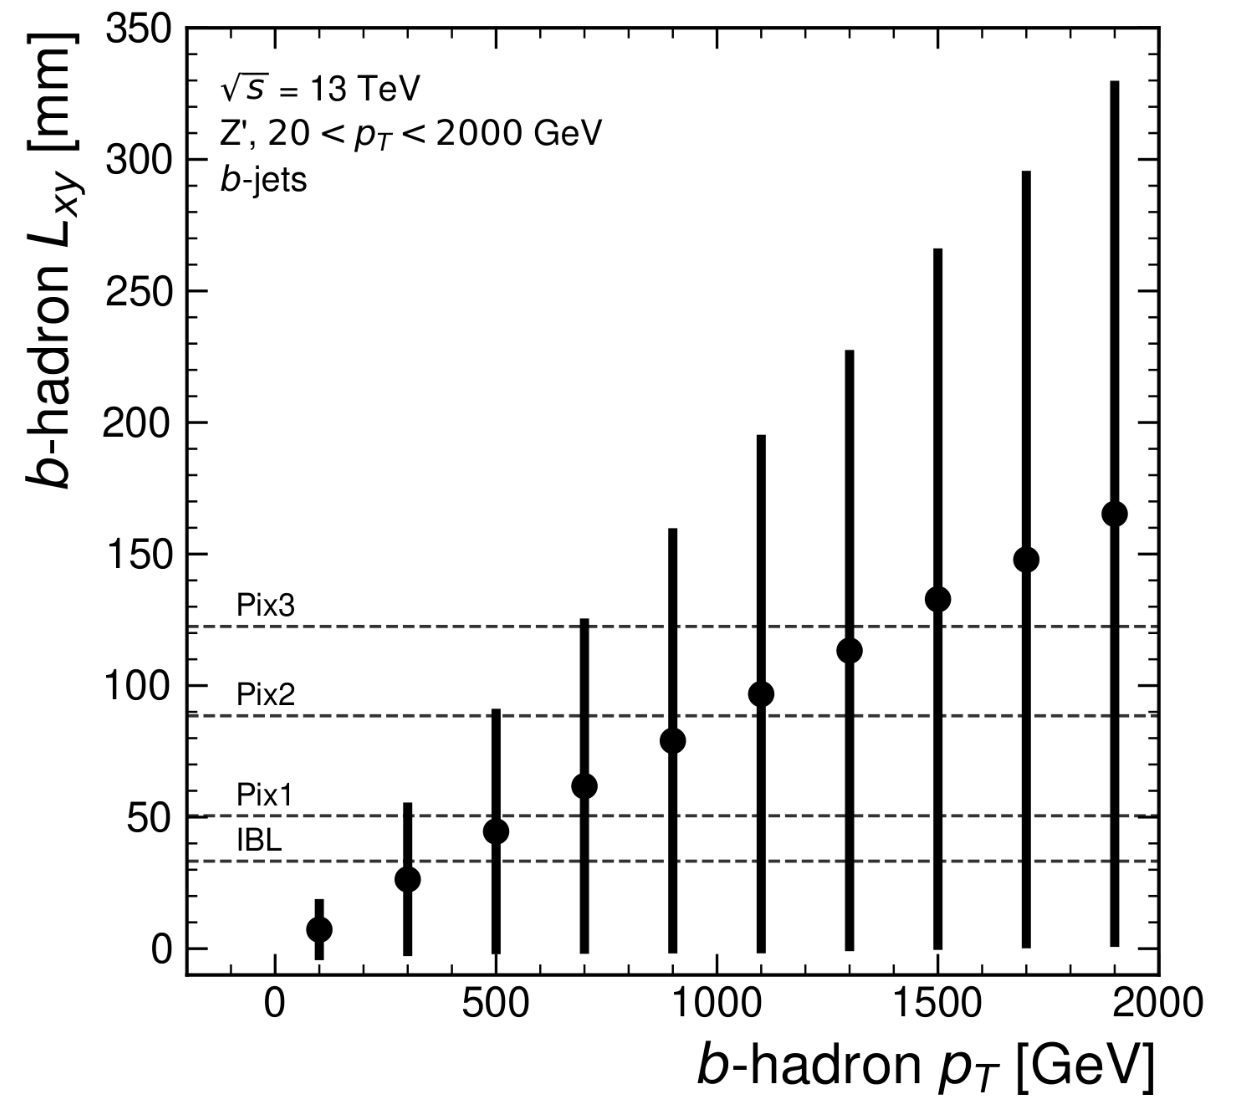
\includegraphics[width=0.98\textwidth]{Images/FTAG/intro/bhaddecay.png}
  \caption{$b$-hadron decay radius as a function of jet $p_T$ reconstructed for $b$-jets in a $Z'$ events with the IBL and pixel layers indicated, from \cite{VanStroud:2869719}. Error bars show the standard deviation of $L_{xy}$ in each $p_T$ bin.} 
  \label{fig:bhaddecay}
\end{subfigure}
\end{figure}

While $b$-jets benefit from an advantageous topology, tagging $c$-jets proves much more challenging as they are at an intermediate scale between light- ($u$, $d$, $s$, and gluons) and heavy flavour jets. A $c$-jet must contain at least one $c$-hadron, from either a $D$-meson (e.g., $D^+=c\bar{d}$, $D^-=d\bar{c}$, $D^0=c\bar{u}$) or a $c$-baryon (e.g., $\Lambda_c^+:udc$). The average decay length for charged (neutral) $D$-mesons, $c\tau_D \sim 300$ $(100)$ $\mu$m \cite{Tanabashi:2018oca}, is smaller than for $b$-hadrons and is harder to resolve with the currently deployed tracker. The decay chain of $b$-hadrons often includes a $c$-hadron, making a clean separation of $c$-jets from $b$-jets harder. Compared to $b$-jets, $c$-jets have a lower final state charged particle multiplicity, on average 4. This lets $\tau$-jets easily being mistaken for $c$-jets, as these leptons can hadronically decay into a similar number of particles to mimic a jet in the detector. For all these reasons, less effort has been historically dedicated to constructing $c$-taggers in ATLAS. The task is however gaining particular attention due to the focus on the challenging $H \rightarrow c\bar{c}$ search \cite{Aaboud:2018fhh, Collaboration:2721696, arXiv:2205.05550}. The focus of this chapter is on the development of novel taggers to identify $b$- and $c$-jet for the ATLAS experiment during the 2020-2024 period, overlaping with the end of Run 2 (2015-2018) analyses and the begining of Run 3 (2022-2026).

\subsection{Flavour Tagging at ATLAS}
In the ATLAS experiment, a choice was made to develop centrally a tagger to be used by the whole collaboration. It relies on a dedicated set of algorithms to perform simultaneously $b$- and $c$-tagging and is continuously improved to meet the requirements of the physics program. Currently, all adopted approaches rely on \gls{dl} methods, given their vastly superior effectiveness. This area of research has been evolving rapidly in recent times due to the community adopting advanced methods from the field of \gls{ai}. As such, various models have been introduced and the last two generations can be split into two categories: 
\begin{enumerate}
  \item The DL1 family are \gls{dl} models built in a hierarchical way. These \gls{dl} methods rely on high-level features reconstructed by sub-algorithms based on physics variables, such as the tracks \glspl{ip}, and the reconstruction of secondary vertices \cite{ATL-PHYS-PUB-2015-022}. The most important models in this family are those including a \gls{dl} sub-model to analyse tracks with either a \gls{rnn} approach for \gls{dl1r} \cite{ATLAS:2017bcq}, leveraging the \gls{rnnip} sub-tagger \cite{ATL-PHYS-PUB-2017-003}, and a Deep Set approaches for \gls{dl1d}, leveraging the \gls{dips} sub-tagger \cite{ATL-PHYS-PUB-2020-014}. This last tagger is, at the moment of writing this thesis, the state-of-the-art deployable tagger for ATLAS in the ATLAS software \cite{ATL-SOFT-PUB-2021-001}. Algorithms from this family were developped for Run 2 of the ATLAS experiment \cite{atlas:FTAGRUN2}, with \gls{dl1d} behind developped towards the end of this data campaign.
  \item The GN family of taggers are built on more advanced \gls{dl} method, as they move away from the hierarchical approach of the DL1 family and directly analyse track and jet information in a unique complex architecture. The GN family is based either on a full Graph Attention Network (\gls{gat}) for \gls{gn1}, and a Transformer encoder for \gls{gn2} \cite{ATL-PHYS-PUB-2022-027, ATL-PLOT-FTAG-2023-01, duperrin2023flavour}. This lighter algorithm pipeline greatly simplifies the maintenance and turnaround time for modification, making the process of updating the taggers nimbler and easier to tailor to specific applications. The GN taggers greatly outperform the DL1 family and represent an exciting area of progress for future analysis requiring precise flavour jets tagging. These methods are being integrated in the ATLAS software stack with objective to be integrated in analyses of the ongoing Run 3 \cite{ATL-SOFT-PUB-2021-001}.  
\end{enumerate}

\begin{figure}[h!]
  \center
  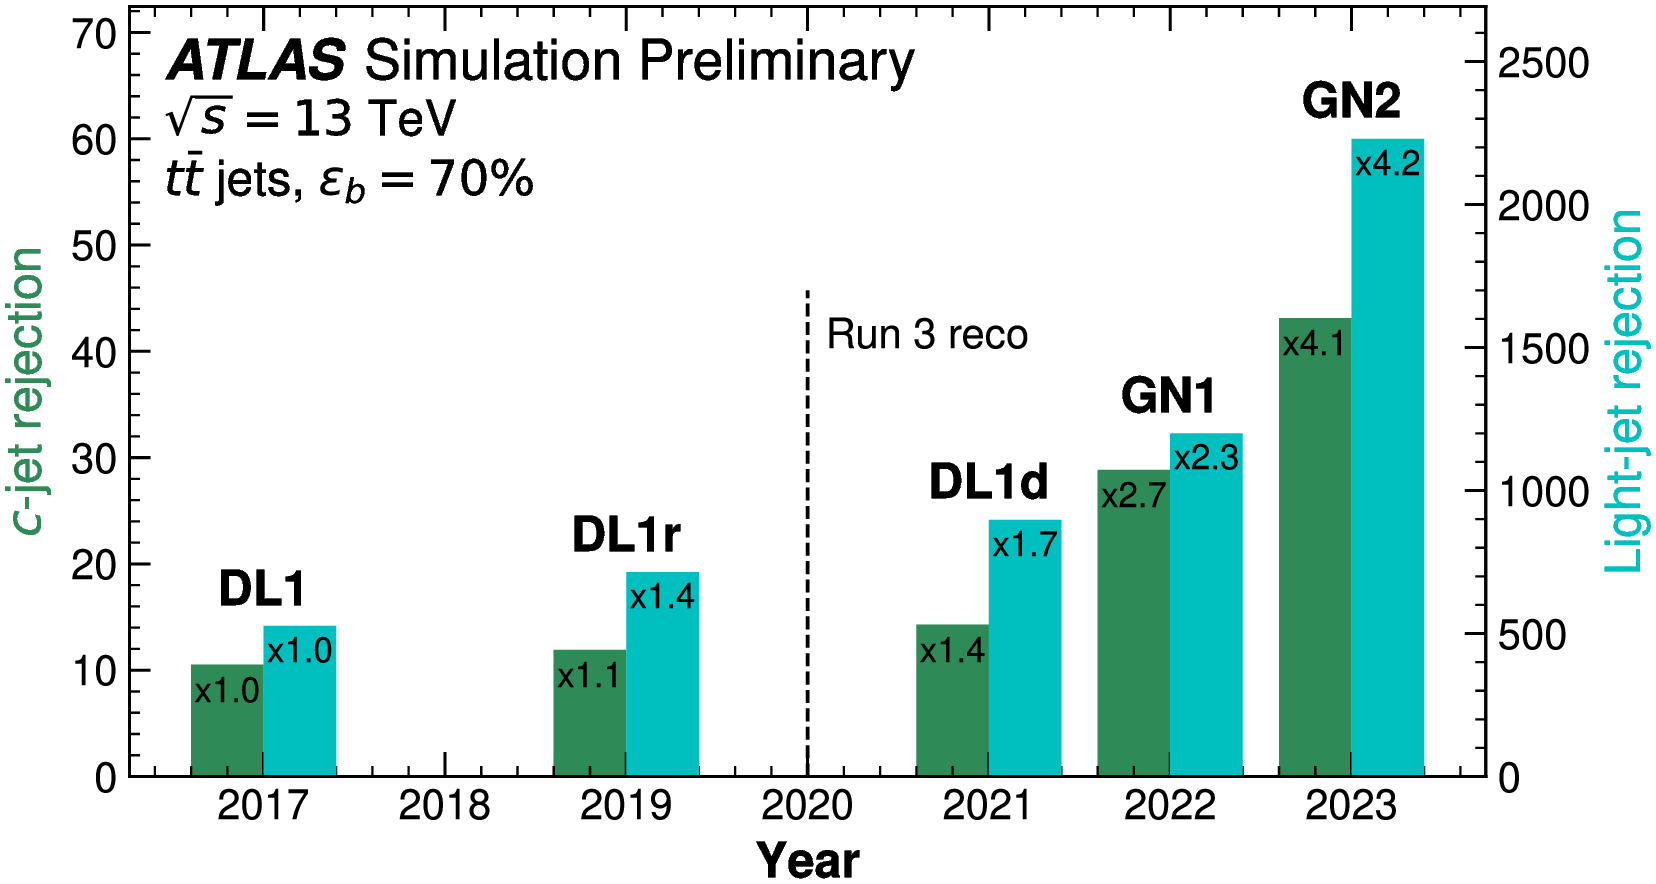
\includegraphics[width=0.8\textwidth]{Images/FTAG/storyFtag.png}
  \caption{Comparison of the performance of flavour tagging models introduced through the years, from \cite{ATL-PLOT-FTAG-2023-01}. Light and $c$-jet rejections are plotted for different taggers at a fixed $b$-jet tagging efficiency of 70\% on a common $t\bar{t}$ evaluation sets. The multiplicative factors in the bars are with respect to the bare DL1 model performance.} 
  \label{fig:storyFtag}
\end{figure}

A historical perspective on the evolution of performance for the different taggers mentioned is presented in Figure \ref{fig:storyFtag}, showing a remarkable continuous increase in light- and $c$-jet rejections at a fixed $b$-tagging efficiency of 70\% on a $t\bar{t}$ dataset. The analysis presented in the latter part of this thesis was carried out in the span of 2021-2024, and was therefore restricted to tools and methods available to the experimental team during this period. As such, due to the need to calibrate the GN taggers as explained latter in Section \ref{chap-calibration} of this chapter, the second family of taggers based on graphs was not yet ready for deployement, making the first family still relevant to explore. Furthemore, some specialised use of flavour taggers and early Run 3 analyses still required the DL1 family, such as the $X_{bb}$ tagger identifying pairs of $b\bar{b}$ and $c\bar{c}$ produced by heavy resonance decays such as a Higgs or a $W$, as described in Section \ref{chap-GN2X}. All the taggers described in this chapter have been integrated in the ATLAS software \cite{ATL-SOFT-PUB-2021-001}. Some early studies of the future performance of the \gls{dl1d} and \gls{gn1} taggers with the updated \gls{itk} detector at the high-luminosity \gls{lhc} as been performed in Ref \cite{ATL-PHYS-PUB-2022-047}.

\subsection{Datasets}\label{ftagdatasets}
The $p_T$ spectrum studied by ATLAS covers a wide range of energies, extending up to 7 TeV. In order to train models able to perform on this large phase space, two datasets are typically combined and described in this section. Each dataset is based from simulated proton-proton collisions at a centre of mass energy $\sqrt{s}$ = 13 TeV. The lower $p_T$ phase space is simulated with the \gls{sm} top-antitop quark pair production $t\bar{t}$ process with at least one $W$ boson produced decaying leptonically, while a \gls{bsm} $Z'$ process is used for the higher momentum region. The latter simulates a modified $Z$ boson from the \gls{sm} with an increased mass to generate a relatively flat jet $p_T$ spectrum of up to 6 TeV. This $Z'$ boson decays in similar proportions to a pair of $b$, $c$, and light-jets. All simulations include realistic effects present in the real data, such as multiple proton-proton interactions per bunch crossing, so-called \glsfirst{pu}, with an average value of $\mu = 40$. Other effects including in the simulations are the detector response from prior and posterior bunch crossing (in-time pile-up) as well the activity from the rest of the event (underlying event). \\

Events in the $t\bar{t}$ samples are simulated using \uppercase{POWHEGBOX V2} generators to next-to-leading (NLO) order in the strong coupling constant $\alpha_s$ \cite{PaoloNason_2004, StefanoFrixione_2007, StefanoFrixione_20072, POWHEGBOX}. The hard scatter matrix element is computed for proton-proton collision with the \uppercase{NNPDF3.0NNLO} set of parton distribution functions (PDF) \cite{PDFLHCrun2}, and the simulated hard scatter events are interfaced with \uppercase{PYTHIA 8.230} \cite{SJOSTRAND2015159} using the A14 parameter tune \cite{ATL-PHYS-PUB-2014-021} and the \uppercase{NNPDF2.3LO} PDFs for the parton shower, hadronisation, and underlying event simulations \cite{BALL2013244}. Studies in Refs \cite{ATL-PHYS-PUB-2016-020, ATL-PHYS-PUB-2020-023} showed these to be the optimal choice to correctly model the top quark $p_T$ and the number of additional jets in the event, with the $h_{\textrm{damp}}$ parameter set at 1.5 the mass of the top-quark $m_{\textrm{top}} = 172.5$ GeV. The $Z'$ events are fully simualted with \uppercase{PYTHIA 8.212}, A14 tune and the \uppercase{NNPDF2.3LO} PDFs. The decays of $b$- and $c$-hadrons are performed by \uppercase{EvtGEN} v1.6.0 \cite{LANGE2001152}. \\

The detector reconstruction effect of ATLAS and the modelling of the interaction between long-lived hadrons and the detector material are simulated with a dedicated software \cite{ATLASSimulationInfra} built on GEANT4 \cite{Agostinelli:602040}. Jets are selected in the phase space region defined by $|\eta| < 2.5$ and $p_T > 20$ GeV, with no overlapping with prompt generator-level $e$ or $\mu$ from the $W$ decay allowed. Pile-up contamination is further reduced by an additional standard selection using the \glsfirst{jvt} algorithm at a tight working point for jets with $p_T < 60$ GeV and $|\eta| < 2.4$ \cite{ATLAS-CONF-2014-018}. Tracks are associated to jets using a $\Delta R$ association cone of width decreasing with $p_T$ ($\Delta R \approx 0.45$ at $p_T =$ 20 GeV and $\Delta R \approx 0.25$ at $p_T > 200$ GeV). Tracks within the cones of several jets are associated to jet with minimal $\Delta R(\textrm{track, jet})$. The label of the jet is inferred from the presence of a truth-level hadron within the cone $\Delta R(\textrm{hadron, jet}) < 0.3$ centred around the jet axis.

\section{DL1 Family of Models: DL1r \& DL1d}
This family of tagger is built with a hierarchical approach, combining low-level algorithms that are independentely optimised into a final \gls{dnn} network of a few layers to output a final prediction. Not all low-level modules are based on \gls{dl}, with some instead directly implementing physics-motivated algorithms. They consist of \cite{Paganini:2289214, atlas:FTAGRUN2}:
\begin{itemize}
  \item \gls{ip} likelihood: IP2D and IP3D are likelihood-ratio templates in 2D and 3D to assign flavour-discriminating weights based, respectively, on the transversal and global impact parameters significance (corresponding to the reweighted \gls{ip} variables by their respective uncertainties) $S_{d_0}$ (35 bins) and $S_{z_0}$ (20 bins) of the tracks, and 14 bins of track catogarisation for IP3D \cite{ATLAS:2017bcq}. For the three flavours, this results in $35 \times 20 \times 14 \times 3 = 29,400$ final bins, which each probability being computed per track. The likelihood assigned to the jet assumes the tracks are independent and is therefore calculated as the product of the per-track likelihoods. A discriminant is derived from the conditional log-likelihood, e.g., $D^b_{IP3D,f} = \sum_{i \in \textrm{tracks}} \log\frac{p_b^i}{p_f^i}$, with $f= c$ or light \cite{ATL-PHYS-PUB-2015-022}.
  \item Track collection analyser: either with \gls{rnnip} \cite{ATL-PHYS-PUB-2017-003} or \gls{dips} \cite{ATL-PHYS-PUB-2020-014}. These are \gls{dl} approaches to extract discrimination information on the set of tracks associated with a jet. These taggers are further described later in this chapter.  
  \item \gls{sv1}: combining a secondary vertex finder and a tagger to offer flavour discrimination information \cite{atlas:FTAGRUN2}. The former, based on the VKalVrt vertex reconstruction package \cite{Kostyukhin:685551}, returns a list of candidate secondary vertices with measured quantities assigned to each vertex. The latter derives jet weights based on discriminative variables and computes properties of the \gls{sv}, such as the mass. 
  \item Jet Fitter: a vertexing algorithm based on a Kalman filter to reconstruct the topology and fit the decay chain \gls{pv} $\rightarrow$ $B$ $\rightarrow$ $D$ with the assumption that the vertices of the weakly decaying B/D-hadrons tend to align with the \gls{pv} \cite{atlas:FTAGRUN2, ATL-PHYS-PUB-2018-025}. 
\end{itemize}

\begin{figure}[h!]
  \centerline{
  \begin{minipage}[c]{0.4\textwidth}
      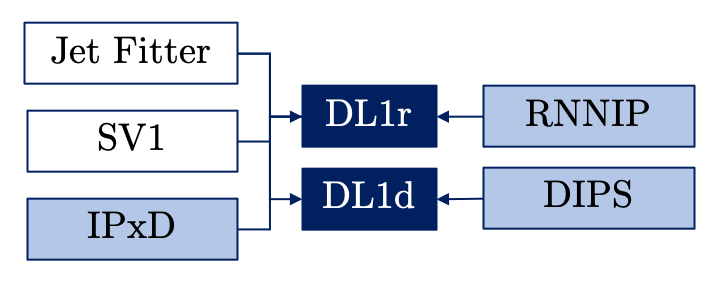
\includegraphics[scale=0.5]{Images/Algorithms}
    \end{minipage}
  \begin{minipage}[c]{0.6\textwidth}
      \caption{The algorithms for flavour tagging at ATLAS. High-level taggers are in dark blue, track-based taggers in light blue and vertex-related taggers in white.}
      \label{fig:algo}
    \end{minipage}
  }
\end{figure}

The outputs of these low-level algorithms, as well as certain jet-related variables, such as $p_T$, are then combined as input to a high-level tagger consisting of a fully-connected \gls{nn} called \gls{dl1r} or \gls{dl1d}, respectively if \gls{rnnip} or \gls{dips} is used. The input vector is typically made of 44-45 features. This high-level tagger outputs three probabilities $p_X$ for the analysed jet to correspond to a $b$-, $c$-, or light--flavour (indicated with the letter $u$) such that $p_b + p_c + p_u = 1$. A $b$-tagging score $D_b$ is then derived by computing a scaled log-likelihood ratio: 
\begin{equation}\label{bdisc}
D_b = \log \frac{p_b}{f^b_c \times p_c + (1 - f^b_c) \times p_u},
\end{equation}
where $f^b_c$ is the charm fraction, a parameter that can be modified to tweak the importance of each flavour. The analogous $c$-tagging score $D_c$ is: 
\begin{equation}\label{cdisc}
D_c = \log \frac{p_c}{f^c_b \times p_b + (1 - f^c_b) \times p_u}.
\end{equation}

A jet is $X$-tagged if the $D_X$ discriminant score is above a set threshold constant $c_{wp}$, defining a \gls{wp} with a unique configuration of signal and background (mis-tag) efficiencies. In this context, the efficiency $\epsilon^X_Y$ for $Y$-flavour jets to be $X$-tagged and the corresponding rejection $\mathcal{R}^X_Y$ are respectively defined as:
\begin{equation}
\epsilon^X_Y = \frac{N^{X-tagged}_{Y-jets}}{N_{Y-jets}} \quad \textrm{and} \quad \mathcal{R}^X_Y = \frac{1}{\epsilon^X_Y},
\end{equation}
where $N^{X-tagged}_{Y-jets}$ and $N_{Y-jets}$ are respectively the number of $X$-tagged $Y$-flavoured jets and the total number of $Y$-flavoured jets. The $f$-rejection is the inverse miss-tagged efficiency of flavour $f$.  \\

These high-level models are trained on \gls{mc} simulated data samples, as mentioned in Section \ref{ftagdatasets}, and need to be calibrated on real data to deliver an unbiased estimate, by deriving \glspl{sf} weights correcting the predictions for each jet as described in Section \ref{chap-calibration}. Uncertainties are derived on the predicted score and passed along to analyses using the tool. The novel algorithm of this family introduced in this work is the \gls{dl1d} tagger, which relies on the \gls{dips} sub-tagger to extract correlations between the tracks.  

\subsection{RNNIP}
The \gls{rnnip} tagger runs on arbitrary-length input sequences made of track features, as ordered by the absolute transverse \gls{ip} significance $|S_{d_0}|$, to extract tagging information from correlations between tracks \cite{ATL-PHYS-PUB-2017-003}. The vector of track features, described in greater details in Table \ref{tab:rnnipVar}, includes the transverse and longitudinal impact parameter significances, the jet $p_T$ fraction carried by the track, the distance between the track and the jet axis, and a learned 2D embedding of the track quality \cite{Paganini:2289214}. It outputs a probability $p_X$ for the jet to belong to flavour $X$ $\in$ [$b$, $c$, light, $\tau$].

\begin{figure}[h!]
  \center
  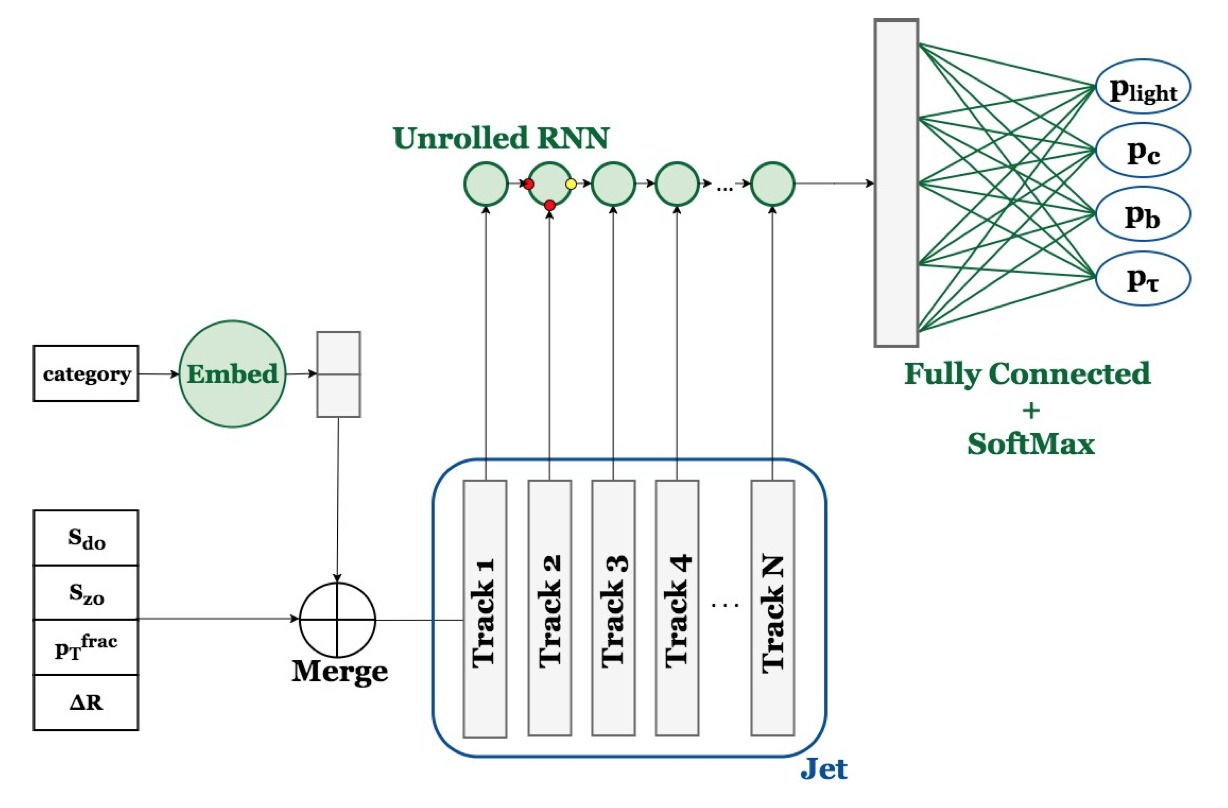
\includegraphics[scale=0.6]{Images/FTAG/rnnip_structure.png}
  \caption{Diagram of the \gls{rnnip} tagger for flavour tagging, from \cite{Paganini:2289214}. The input consists in track features augmented with an embedding of track categories. Tracks are then ordered by absolute transverse \gls{ip} significance and fed through an \gls{lstm} core. The unrolled sequence outputed from this \gls{lstm} is padded to a fixed size and processed by a \gls{dnn} to output the per-flavour probabilities.} 
  \label{fig:rnnipModel}
\end{figure}

The architecture of \gls{rnnip} is a \gls{rnn}-based model leveraging an \gls{lstm} core, as depicted in Figure \ref{fig:rnnipModel}. The arbitrary-length sequence fed as input is mapped by the \gls{lstm} cell with a 100-unit hidden layer into a 50-dimensional vector. This vector is then processed by a 20-unit fully-connected feed-forward neural network outputing the per-flavour probabilities by computing the softmax of the last layer's output. To avoid overfitting, a dropout value of 0.2 is applied to the \gls{lstm} cell. 

\begin{table}[h]
  \begin{center}
      \begin{tabular}{C{3cm}|C{13cm}} 
      	 \hline \hline
          Track Variables & Description  \\ \hline \hline
          $S_{d_0}$      & Lifetime signed transverse \gls{ip} significance $d_0 / \sigma_{d_0}$, with $d_0$ the transverse \gls{ip} - the transverse distance from the \gls{pv} to the point of closest approach (perigee) of the track - and $\sigma_{d_0}$ the error on $d_0$. If the perigee is in front (behind) the \gls{pv} with respect to the jet direction, the sign is positive (negative). \\ \hline
          $S_{z_0}$      & Lifetime signed longitudinal \gls{ip} significance $z_0 / \sigma_{z_0}$, with $z_0$ the longitudinal \gls{ip} - the longitudinal distance from the \gls{pv} to the perigee of the track - and $\sigma_{z_0}$ the error on $z_0$. A sign is assigned as per the prescription of $S_{d_0}$. \\ \hline
          $p_T^{\textrm{frac}}$   & Fraction of the reconstructed jet $p_T^{\textrm{jet}}$ carried by the track $p_T^{\textrm{frac}} = p_T^{\textrm{track}} / p_T^{\textrm{jet}}$. \\ \hline
          $\Delta R$(track, jet) & Geometrical distance in 2D angle between the track direction and jet axis $\Delta R = \sqrt{(\phi_{\textrm{track}} - \phi_{\textrm{jet}})^2 + (\eta_{\textrm{track} - \eta_{\textrm{jet}}})^2}$. \\ \hline
          Category       & 2D representation of the track quality learnt by an embedding layer. The categorisation is based on the number of observed, expected and missing hits in the different layers of the tracker (silicon pixel and strip detectors) \cite{ATL-PHYS-PUB-2015-022}.  \\ \hline
      \end{tabular}
    \caption{Track variables passed to the initial version of the \gls{rnnip} model \cite{ATL-PHYS-PUB-2017-003}. Later versions removed the category embedding and added the per-track hit information shown for \gls{dips} in Table \ref{tab:dipsVar}.}
    \label{tab:rnnipVar}
  \end{center}
\end{table}

\gls{rnnip} is designed to capture correlations between the tracks of a jet, a rich information explicitely missing from the \gls{ip}-based discriminant of IP2D and IP3D due to the factorisation of the likelihood. Some degree of correlation is expected between tracks, as these can emerge from the same secondary or tertiary vertex of the displaced decay in $b$- and $c$-jets. It removes the cumbersome procedure to built likelihood templates, which demands large amount of data to scale to finer bin resolution and is computationally expensive due to the number of bins scaling exponentially with the number of variables. Early tests showed that \gls{rnnip} is effective at building a discriminant, delivering superior performances to the \gls{ip}-based approaches with only $\sim$40 \% of the parameters - 11,636 trainable parameters for \gls{rnnip} \cite{Paganini:2289214}.

\subsection{DIPS}
The \gls{dips} tagger, based on the Deep Set architecture \cite{NIPS2017f22e4747} and depicted in Figure \ref{fig:dipsModel}, is a \gls{gnn}-based alternative approach to \gls{rnnip} to model the correlations between an arbitrary number of tracks \cite{ATL-PHYS-PUB-2020-014}. As introduced in Chapter \ref{chapter-GNN}, such a model is composed of two fully-connected feed-forward neural network. A first \gls{dnn} called the \textit{track network} $\Phi$ maps each individual track feature vector - similar to the input of \gls{rnnip} - to a latent space representing the nodes of a graph. The representations of each track in this latent space are then pooled by a simple summation operation - representing the unweighted edges of a fully connected graph - and given as input to a secondary \gls{dnn}, called the \textit{jet network} $F$, outputting the predicted probability $p_X$ for the jet to belong to flavour $X$ $\in$ [$b$, $c$, light, $\tau$]. This last network represents the global attribute of the graph $u$, in the notation of Chapter \ref{chapter-GNN}. 
In summary, \gls{dips} computes the following equation on the set of track features $\{ p_i \}$, with $i = 1, ..., N$ for arbitrarily-sized jets of $N$ tracks:
\begin{equation}
  DIPS( \{p_1, ..., p_N \} ) = F\left( \sum_{i=1}^N \Phi(p_i) \right),
\end{equation}
to output the per-flavour probabilities. The separation of computation into a per-track embedding and a per-jet processing after a size-indepent pooling performed by the sumation operator allows the model to process unordered sets of variable size. The track features used as inputs are described in Table \ref{tab:dipsVar}, with only the top 15 tracks as ranked by decreasing $S_{d_0}$ being kept.

\begin{figure}[h!]
  \center
  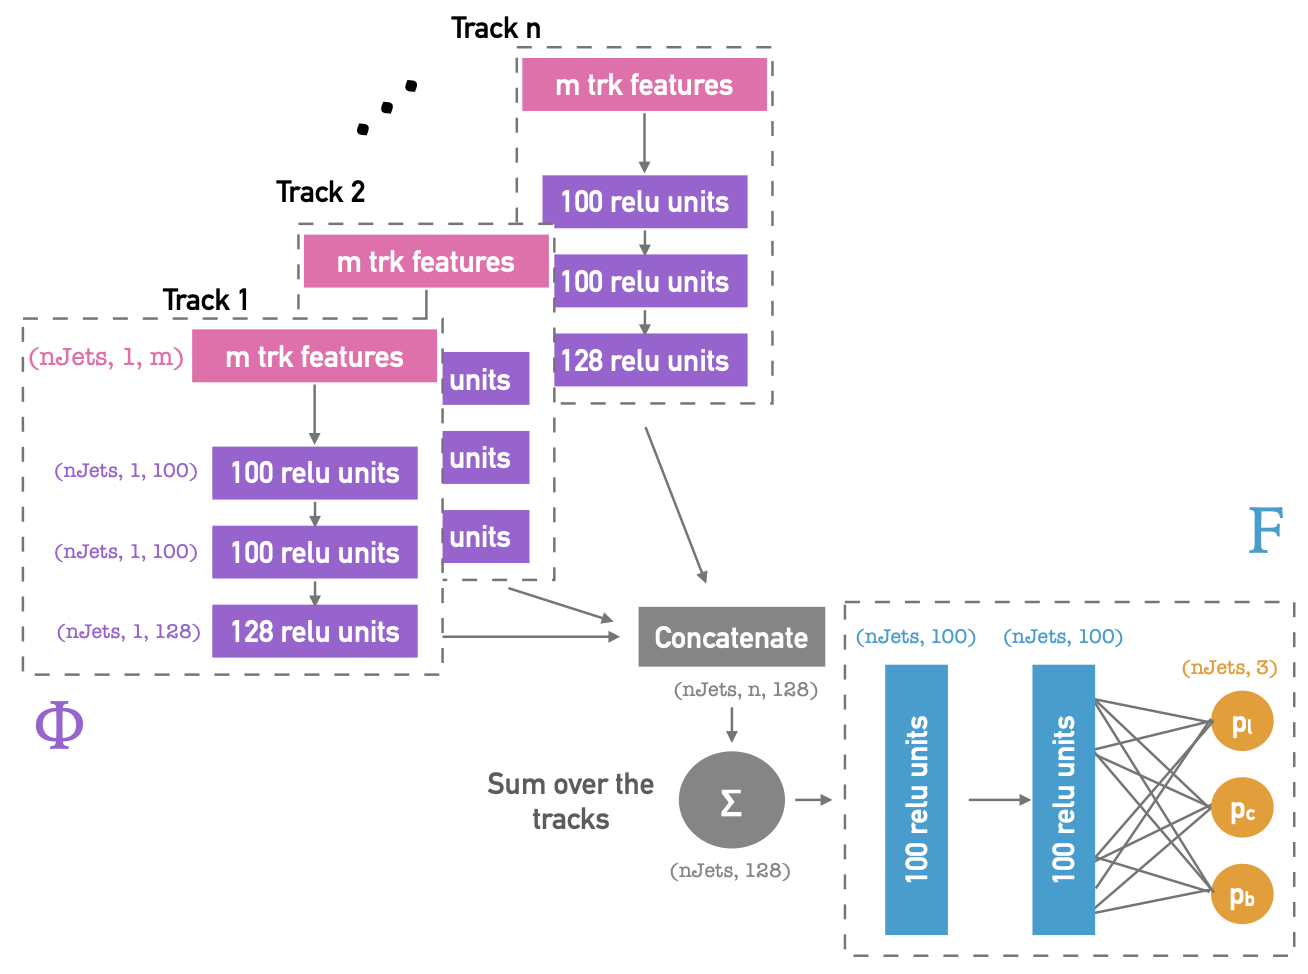
\includegraphics[scale=0.6]{Images/FTAG/dips_structure.png}
  \caption{Diagram of the \gls{dips} tagger for flavour tagging, from \cite{ATL-PHYS-PUB-2020-014}. The input consists in a set of $N$ tracks each represented by a feature vector. Each track is embedded by a \gls{dnn} track network $\Phi$ into a fixed-dimension vector. All embedded track vectors are then pooled by summation to a fixed-size vector. The last step is to process this vector with another \gls{dnn} jet network $F$ outputing the per-flavour probabilities. The number and width of layers presented here are the nominal architecture.} 
  \label{fig:dipsModel}
\end{figure}

\begin{table}[h]
  \begin{center}
      \begin{tabular}{C{3cm}|C{13cm}} 
      	 \hline \hline
          Variables & Description  \\ \hline
          $S_{d_0}$      & Lifetime signed transverse \gls{ip} significance $d_0 / \sigma_{d_0}$, with $d_0$ the transverse \gls{ip} - the transverse distance from the \gls{pv} to the point of closest approach (perigee) of the track - and $\sigma_{d_0}$ the error on $d_0$. If the perigee is in front (behind) the \gls{pv} with respect to the jet direction, the sign is positive (negative). \\ \hline
          $S_{z_0}$      & Lifetime signed longitudinal \gls{ip} significance $z_0 / \sigma_{z_0}$, with $z_0$ the longitudinal \gls{ip} - the longitudinal distance from the \gls{pv} to the perigee of the track - and $\sigma_{z_0}$ the error on $z_0$. A sign is assigned as per the prescription of $S_{d_0}$. \\ \hline
          $\log p_T^{\textrm{frac}}$   & Logarithm of the fraction of the reconstructed jet $p_T^{\textrm{jet}}$ carried by the track $\log p_T^{\textrm{frac}} = \log p_T^{\textrm{track}} / p_T^{\textrm{jet}}$. \\ \hline
          $\log \Delta R$(track, jet) & Logarithm of the geometrical distance in 2D angle between the track direction and jet axis $\log \Delta R = \log \sqrt{(\phi_{\textrm{track}} - \phi_{\textrm{jet}})^2 + (\eta_{\textrm{track} - \eta_{\textrm{jet}}})^2}$. \\ \hline
          IBL hits      & Number of hits recorded in the \gls{ibl} - 0, 1, or 2. \\ \hline
          PIX1 hits       & Number of hits in the innermost pixel layer, after the \gls{ibl} - 0, 1, or 2.  \\ \hline
          Shared IBL hits & Number of hits in the \gls{ibl} that are shared by more than one track. \\ \hline
          Split IBL hits  & Number of split hits in the \gls{ibl}, that are created by multiple charged particles. \\ \hline
          nPixHits        & Total number of hits in all the pixel layers.\\ \hline
          Shared pixel hits & Number of shared hits in the pixel layers.\\ \hline
          Split pixel hits  & Number of split hits in the pixel layers.\\ \hline
          nSCTHits          & Total number of hits in the \gls{sct} layers. \\ \hline
          Shared SCT hits   & Number of shared hits in the \gls{sct} layers.\\ \hline \hline
      \end{tabular}
      \caption{Track variables passed to the \gls{dips} model and later versions of the \gls{rnnip} model \cite{ATL-PHYS-PUB-2020-014}. Compared to the initial \gls{rnnip} variables of Table \ref{tab:rnnipVar}, the $p_T^{\textrm{frac}}$ and $\Delta R$ are passed as log values to reduce the magnitude of the long tail observed at large values and improve the training time. Shared hits are hits used by multiple tracks without being classific as split by a dedicated cluster-splitting \gls{nn} \cite{ATLAS-tracks-algo}.}
    \label{tab:dipsVar}
  \end{center}
\end{table}

This approach has several advantages over \gls{rnnip}, mainly the physically motivated permutation-invariance of the input and the improved training and evaluation time thanks to a more parallelisable architecture, as the track embedding performed by $\Phi$ can be massively parallalised on \gls{gpu}. These motivations are translated in an appreciable performance delivered by \gls{dips}, which is observed to globally outpeform version of \gls{rnnip} using the same variables, while operating at a reduced computational cost \cite{ATL-PHYS-PUB-2020-014}. The performance can be assessed from Figure \ref{fig:dipsrnnipPerf}, presenting the \gls{roc} curves for baselines trainings of \gls{dips} and \gls{rnnip} in terms of light- and $c$-rejection for $b$-jet tagging on the same held-out $t\bar{t}$ evaluation sample.

\begin{figure}[h!]
  \centering
  \begin{subfigure}[b]{0.48\textwidth}
      \centering
      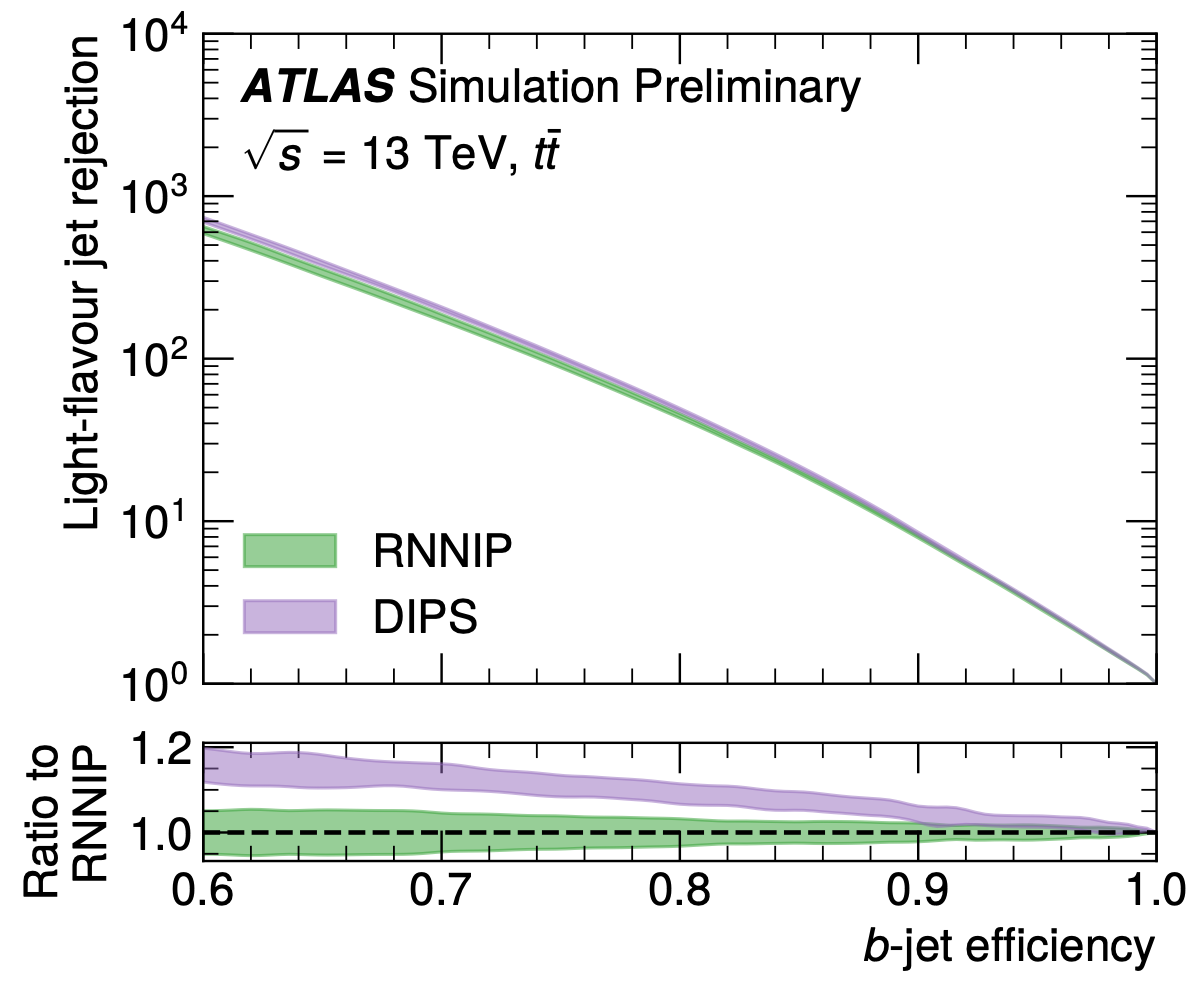
\includegraphics[width=0.98\textwidth]{Images/FTAG/dipsrnnipL.png}
      \caption{Light-rejection.} 
      \label{fig:dipsrnnipPerfL}
  \end{subfigure}
  \hfill
  \begin{subfigure}[b]{0.48\textwidth}
      \centering
      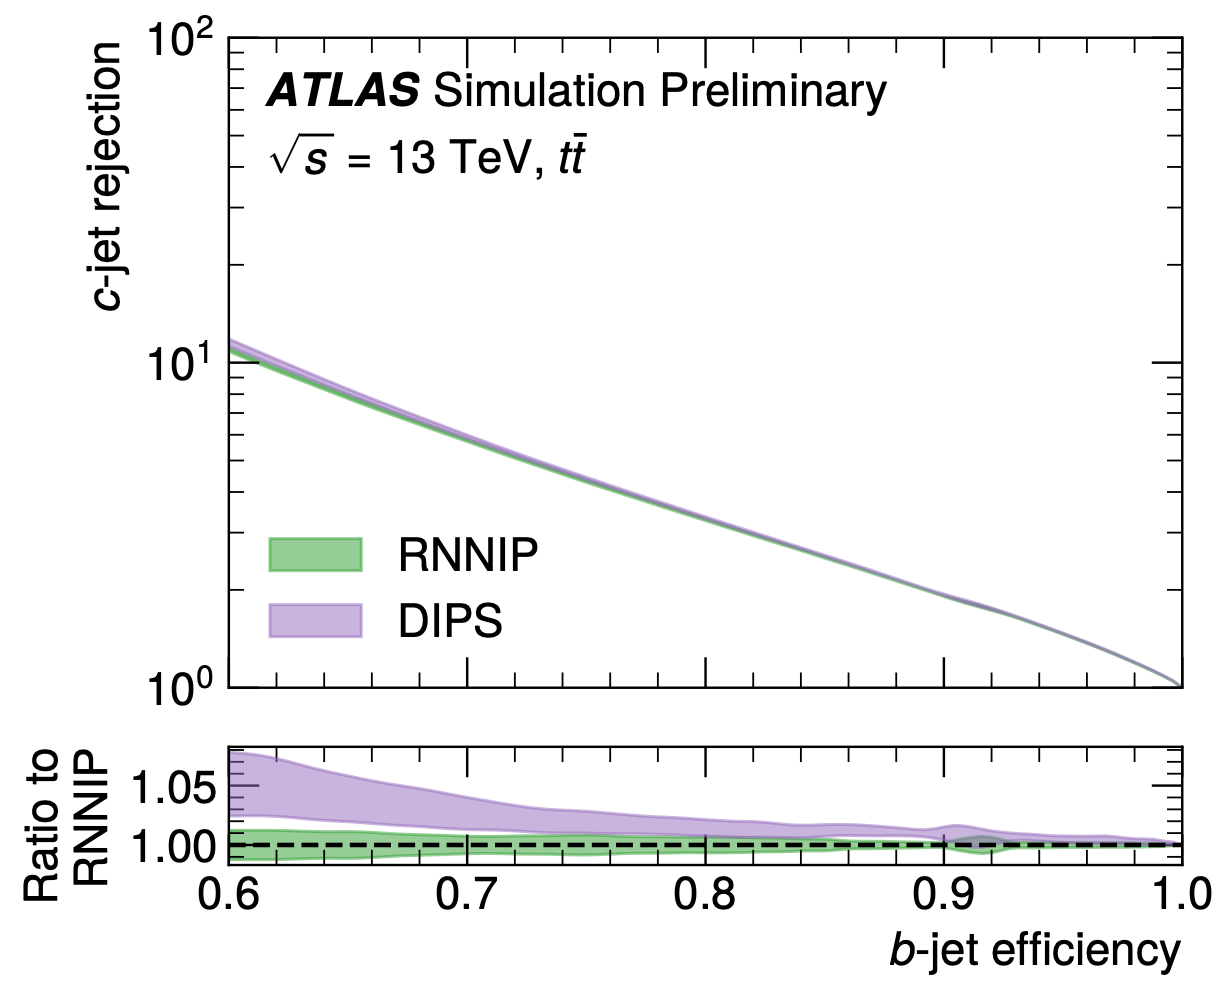
\includegraphics[width=0.98\textwidth]{Images/FTAG/dipsrnnipC.png}
      \caption{$c$-rejection.} 
      \label{fig:dipsrnnipPerfC}
  \end{subfigure}
  \caption{Light- (left) and $c$-rejection (right) as a function of $b$-jet tagging efficiency for \gls{rnnip} (green) and \gls{dips} (purple), taken from \cite{ATL-PHYS-PUB-2020-014}. Each curve and error bands show, respectively, the mean and standard deviation of the rejections for 5 trainings per algorithm. The bottom panel shows the ratio with respect to \gls{rnnip}, showing a clear performance gain for \gls{dips} at all $b$-jet efficiency considered.}
  \label{fig:dipsrnnipPerf}
\end{figure} 

The training times on the same \gls{gpu} hardware for a 48k parameters \gls{dips} model is estimated to take 78 $\pm$ 4 seconds per epoch - averaging over 5 seeds - while a 47k parameters \gls{rnnip} requires roughly thrice as much, 241 $\pm$ 14 seconds per epoch \cite{ATL-PHYS-PUB-2020-014}. The faster training time allowed the Collaboration to focus on optimisation studies of the hyperparameters. The optimisation campaign focused on three aspects of the \gls{dips} network: the architecture of the two \gls{nn}, the track selection, and the set of trac features used as input in addition to those of Table \ref{tab:dipsVar}. Regarding architecture, a grid search over various possible values for the number of layers in $\Phi$ and $F$, number of nodes, and the dimension of the track embedding space showed no significant performance change. The selected architecture is:
\begin{itemize}
  \item Track network $\Phi$: three layers of 100, 100, and 128 units applied to each track. 
  \item Jet network $F$: four layers of size 100, 100, 100, 30 before the final output of size dictated by the number of flavour to identify. 
\end{itemize}
To regularise and avoid overfitting, both batch normalisation and dropout were tested with the former observed to give better results. \\ 

The second optimisation step however uncovered that a variation to the track selection does offer opportunities for improved performance. Jets are reconstructed with the anti-kT algorithm with a radius of R = 0.4. For \gls{rnnip}, IP2D, and IP3D, the selected tracks must pass the following quality selection: $\geq$ 7 hits in the silicon layers, $\leq$ 2 missing hits in the silicon layers, $\geq$ 1 hit in the pixel detector, $\leq$ 1 hit shared by multiple tracks, $p_T$ > 1 GeV, $|d_0|$ < 1 mm, and $|z_0 \textrm{ sin}(\theta)|$ < 1.5 mm. For \gls{dips}, a looser track selection increasing the acceptance of the last three cuts was studied, modifying the nominal selection in the following way: $p_T$ > 0.5 GeV, $|d_0|$ < 3.5 mm, and $|z_0 \textrm{ sin}(\theta)|$ < 5 mm \cite{ATL-PHYS-PUB-2020-014}. Loosening the selection and keeping the top 25 tracks as ranked by decreasing $S_{d°0}$ to capture more tracks from heavy flavour decays was observed to lead to a significant improvement in performance for jets with a $p_T < 250$ GeV for \gls{dips}. From an \gls{ml} viewpoint, a larger set of input information with more noise can still prove beneficial if the underlying model is complex enough to capture useful features in the noisy data, that would otherwise be erased by a more stringent selection. The performance gain from this loosened selection-trained \gls{dips} is displayed in the \gls{roc} curves of Figure \ref{fig:dipsOptRoc}. \\

\begin{figure}[h!]
  \centering
  \begin{subfigure}[b]{0.48\textwidth}
      \centering
      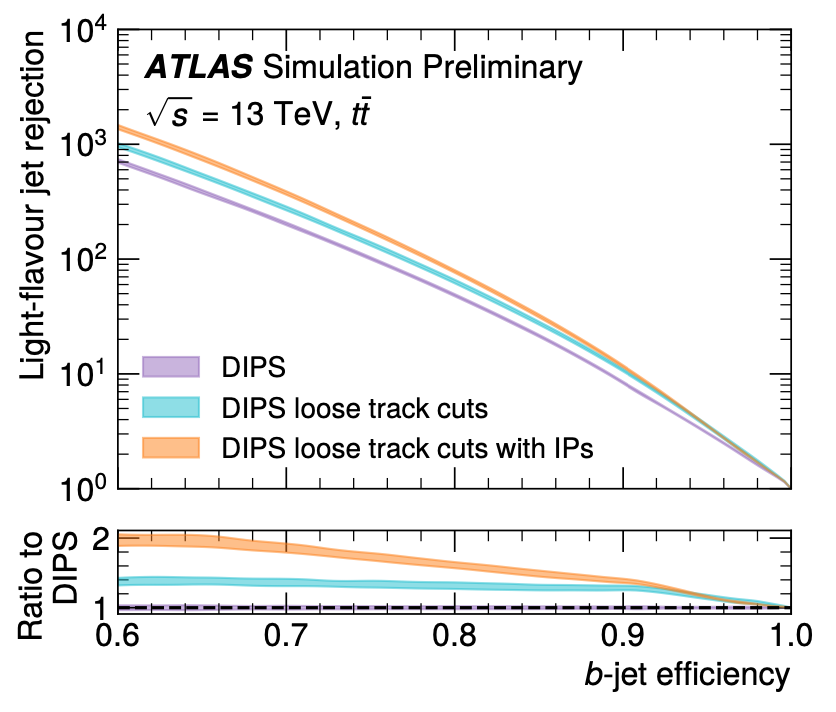
\includegraphics[width=0.98\textwidth]{Images/FTAG/dipsOptL.png}
      \caption{Light-rejection.} 
      \label{fig:dipsOptRocL}
  \end{subfigure}
  \hfill
  \begin{subfigure}[b]{0.48\textwidth}
      \centering
      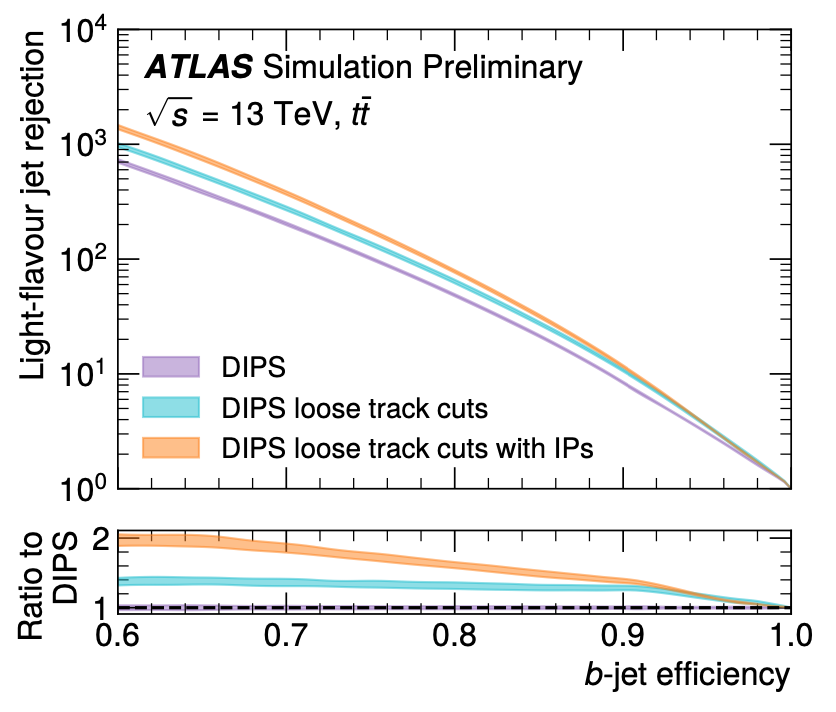
\includegraphics[width=0.98\textwidth]{Images/FTAG/dipsOptL.png}
      \caption{$c$-rejection.} 
      \label{fig:dipsOptRocC}
  \end{subfigure}
  \caption{Light- (left) and $c$-rejection (right) as a function of $b$-jet tagging efficiency for different \gls{dips} model, with the baseline (nominal) \gls{dips} in purple, the loosened track selection in blue, and the fully optimised \gls{dips} in orange, from \cite{ATL-PHYS-PUB-2020-014}. The curve and error bands show, respectively, the mean and standard deviation of the rejections for 5 trainings per algorithm with different initial random seed. The bottom panel shows the ratio with respect to the baseline \gls{dips}, showing a clear performance gain from the two steps optimisation procedure at all $b$-jet efficiency considered.}
  \label{fig:dipsOptRoc}
\end{figure} 

Furthemore, clear benefits are obtained when adding additional track features as input on top of the looser selection, as shown by the orange curve of Figure \ref{fig:dipsOptRoc}, which plots the performance of a loose track selection \gls{dips} trained with the per-track \gls{ip} parameters $d_0$ and $z_0$ in addition to the features of Table \ref{tab:dipsVar}.

\begin{figure}[h!]
  \center
  \begin{minipage}[c]{0.7\textwidth}
    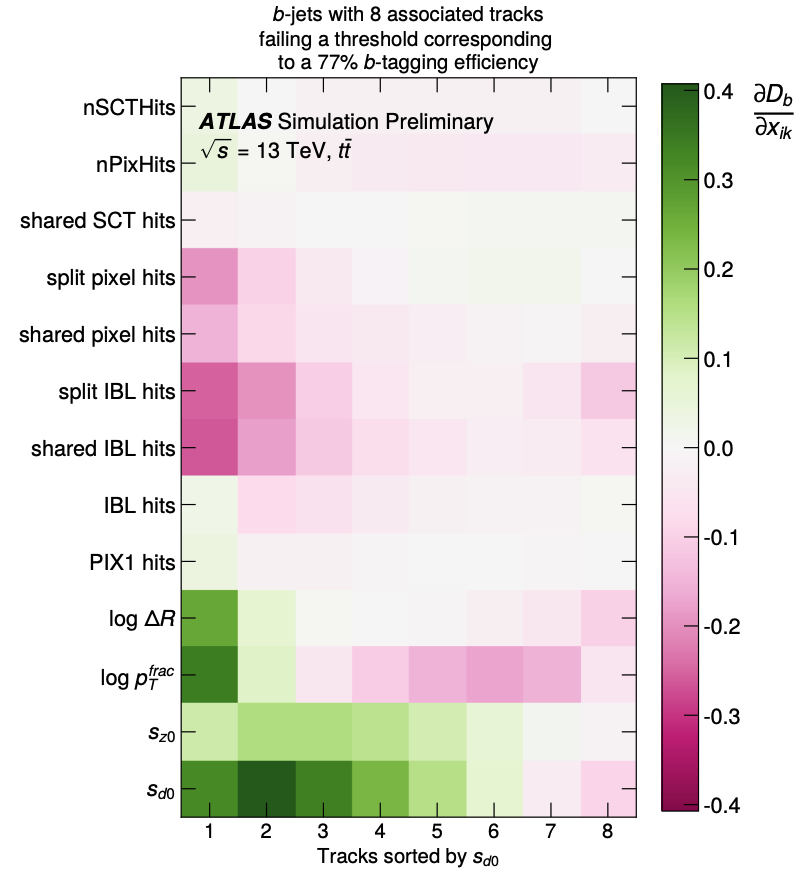
\includegraphics[width=\textwidth]{Images/FTAG/dipsSaliency.png}
  \end{minipage}
  \begin{minipage}[c]{0.25\textwidth}
    \caption{Saliency map for $b$-tagging with 8 tracks sorted by $|S_{d_0}|$, showing the gradient of the discrimant $D_b$ with respect to the track features $x_{ik}$ displayed on the $y$-axis \cite{ATL-PHYS-PUB-2020-014}.} 
  \label{fig:dipsSaliency}
  \end{minipage}
\end{figure}

How does \gls{dips} work? Interpretability of machine learning models is an active area of research. Several effective approaches exist to gauge the importance of the input on the prediction, such as Shapley values. Figure \ref{fig:dipsSaliency} presents an alternative technique called \textit{saliency maps} \cite{Simonyan2013DeepIC}. Using the $b$-tagging discriminant $D_b$ of Equation \ref{bdisc} at a fixed efficiency of 77\%, the average importance of each feature in the track inputs is assessed by averaging the gradient of the discriminant with respect to the track feature over a set of $N$ jets with strictly 8 associated tracks failing the threshold:
\begin{equation}
  \frac{\partial D_b}{\partial x_{ik}} = \frac{1}{N} \sum_{j=1}^N \frac{\partial D_b^{j}}{\partial x_{ik}^{j}},
\end{equation} 
where $i$ indexes the 8 tracks, $j$ indexes the jet in the sample of size $N$, $x_{ik}$ is the $k^{th}$ feature of the $i^{th}$ jet \cite{ATL-PHYS-PUB-2020-014}. This process effectively indicates the linear sensitivity of the discriminant on the track features. Using the saliency map, one can infer what features to modify to correct the failed tagged assigned to the $b$-jets sample. The most sensitive parameters are measured to be the \gls{ip} significances of the first five tracks, and the logarithm of the $p_T^{\textrm{frac}}$ and $\Delta R$ of the track with largest $|s_{d_0}|$. This observation is physically motivated by the dynamic of the harder fragmentation of $b$-quarks, compared to light- and $c$-quarks. Negative gradients are measured for shared and split hits observables, translating into a further incorrect discriminant under linear change of these features. This is also physically motivated, as higher count typically trace back to denser environment where random combinations of hits to form tracks are more likely. However, total hit counts in the different tracker layers have a small positive impact, as these correlate with the reconstruction of the \gls{ip} parameters.

\subsection{Training of DIPS with Variable Radius Jets for Run 3}\label{chapter:dipsVRtrain}
The physics program of the ATLAS Collaboration covers a wide range of analyses, targeting different topologies and processes at different energies. With respect to flavour tagging, a particularly relevant aspect is the energy or tranverse momenta of the jets to label. Indeed, flavour tagger are extremely sensitive to the dynamic of the underlying events. At higher energies, corresponding to higher momenta of the hadronised quark or gluon, the jet constituents emenating from the decaying parton tend to be more collimated in the same direction, as they have to share a high initial energy between themselves. This topology confends tracks and blends the rich internal jet dynamics in the measured signature, making tracks separation and secondary or tertiary vertex identification more difficult. Analyses targeting jets from hadronic or semileptonic decays of heavy particles, such as the top $t$-quark, Higgs, or the gauge bosons $W/Z$, can easily produce such highly energetic or \textit{boosted} jets.  \\

So far in this chapter, mentions of ``jets'' were always referring to the object as reconstructed by the anti-$k_T$ algorithm with a fixed radius $R = 0.4$ applied to PFLow objects, as introduced in Chapter \ref{chapter-ATLAS}. This reconstruction method proves robust in the hadron collider setting as it both leads to suitably-shaped jet structure and \gls{pu}-removing properties. This fixed radius however becomes a hurdle for boosted jet, as their average radius decreases with energy due to the collimation of the jet components. Indeed, the angular separation $\Delta R = \sqrt(\Delta\eta^2 + \Delta \phi^2)$ between the products of a decaying particle $X$ of large mass $m_X$ scales inversely to the transverse momentum \cite{ATLAS:largeRjet}: 
\begin{equation}\label{eq:sizeJet}
  \Delta R \approx \frac{2 m_X}{p_T^X}.
\end{equation}
At low $p_T^X$, the individually produced particle from the decay are sufficiently separated to be reconstructed as individual objects, hence the \textit{resolved} regime label \cite{ATLAS:2016hcf}. For example, a non-boosted Higgs decaying to a $b\bar{b}$ pair can be reconstructed as two $b$-jets with small $R$. At higher momentum however, the content of the decay is collimated and overlaps: this is the \textit{boosted} regime. The decaying particle $X$ in such a regime is typically reconstructed as a single large radius jets, to catch the different underlying jets, for example with the anti-$k_T$ method with radius $R = 1.0$. Using such a fixed large radius overestimates the size of boosted jets which are easily contaminated by the \gls{pu}, as well as the underlying event and initial-state radiations.  \\

A novel approach to model jets from boosted object decays is to reconstruct them with \gls{vr} jet algorithm \cite{vrJetPaper}, as introduced in Chapter \ref{chapter-ATLAS}. \gls{vr} jets have a size that scales with the inverse of the reconstructed jet momentum, thus correctly following the expected dynamic of Equation \ref{eq:sizeJet}. Such a significant change to the jet reconstruction is bound to have an impact on algorithms learning structure from the jet contents, as is the case of all deep learning-based taggers presented in this chapter. These models have therefore to be fine-tuned seperately to this new jet-type for optimal performance, which is the focus of this section. \\  % Chapter with VR JET

For the \gls{vr}-training, the dataset is composed of three samples simulating proton-proton collisions at $\sqrt{s} = 13$ with the following fractions:
\begin{enumerate}
  \item 85 \% of jets are sampled from the $t\bar{t}$ with a maximal $p_T$ of 400 GeV. At least one of the $W$-boson from the $t$-quark is required to decay leptonically.
  \item 7.5\% are sampled from $Z'$ events, where an exotic boson $Z'$ decays as $Z' \rightarrow q\bar{q} \textrm{ or } \tau \bar{\tau}$, with a variable $Z'$ mass to generate a flat $p_T$ spectrum extending the $p_T$-range of the jets studied up to 4 TeV. These jets are required to have a $p_T > 150$ GeV.
  \item 7.5\% are sampled from a simulated graviton process to also increase the range towards higher momenta. These jets are required to have a $p_T > 150$ GeV.
\end{enumerate}

The simulation process is similar to that introduced in Section \ref{ftagdatasets}. Figure \ref{fig:vrjetdist} displays the jet $p_T$ and $|\eta|$ distributions for the hybrid sample as well as the individual samples it is based upon, for a total of 40 $\times$ $10^6$ jets per flavour in \{$b$, $c$, light\}. In order to reach such high statistics, importance sampling is used to over-sample the limited amount of $c$-jets while using all available $b$- and downsampling light-jets. A particularity of the processing is the requirement for the $p_T$ and $|\eta|$ spectra to be equally-distributed for all jet flavours, so that these features arising from inherent physics effects in the specific processes simulated cannot be used by the model to discriminate between flavours. The technique implemented is importance sampling with replacement. It selects jets of different flavours to match a target distribution. The importance sampling weights are derived by first deriving the ratio of the target 2D distribution to the per flavour one. Weights above 1 indicate jets in the $i, j$ bin have to be oversampled, while values lower than 1 indicate the typical downsampling requirement. Jets are then iteratively sampled until the sampled distribution of each flavour individually matches the target distribution. As displayed in Figure \ref{fig:vrjetdisth} for which the target were $b$-jets, the thus constructed distribution as the same $p_T$ and $|\eta|$ distributions for all flavours. This work introduced to the first implementation of the importance sampling method, now widely used to develop flavour tagging tools.  

\begin{figure}[h!]
  \centering
  \begin{subfigure}[b]{0.98\textwidth}
      \centering
      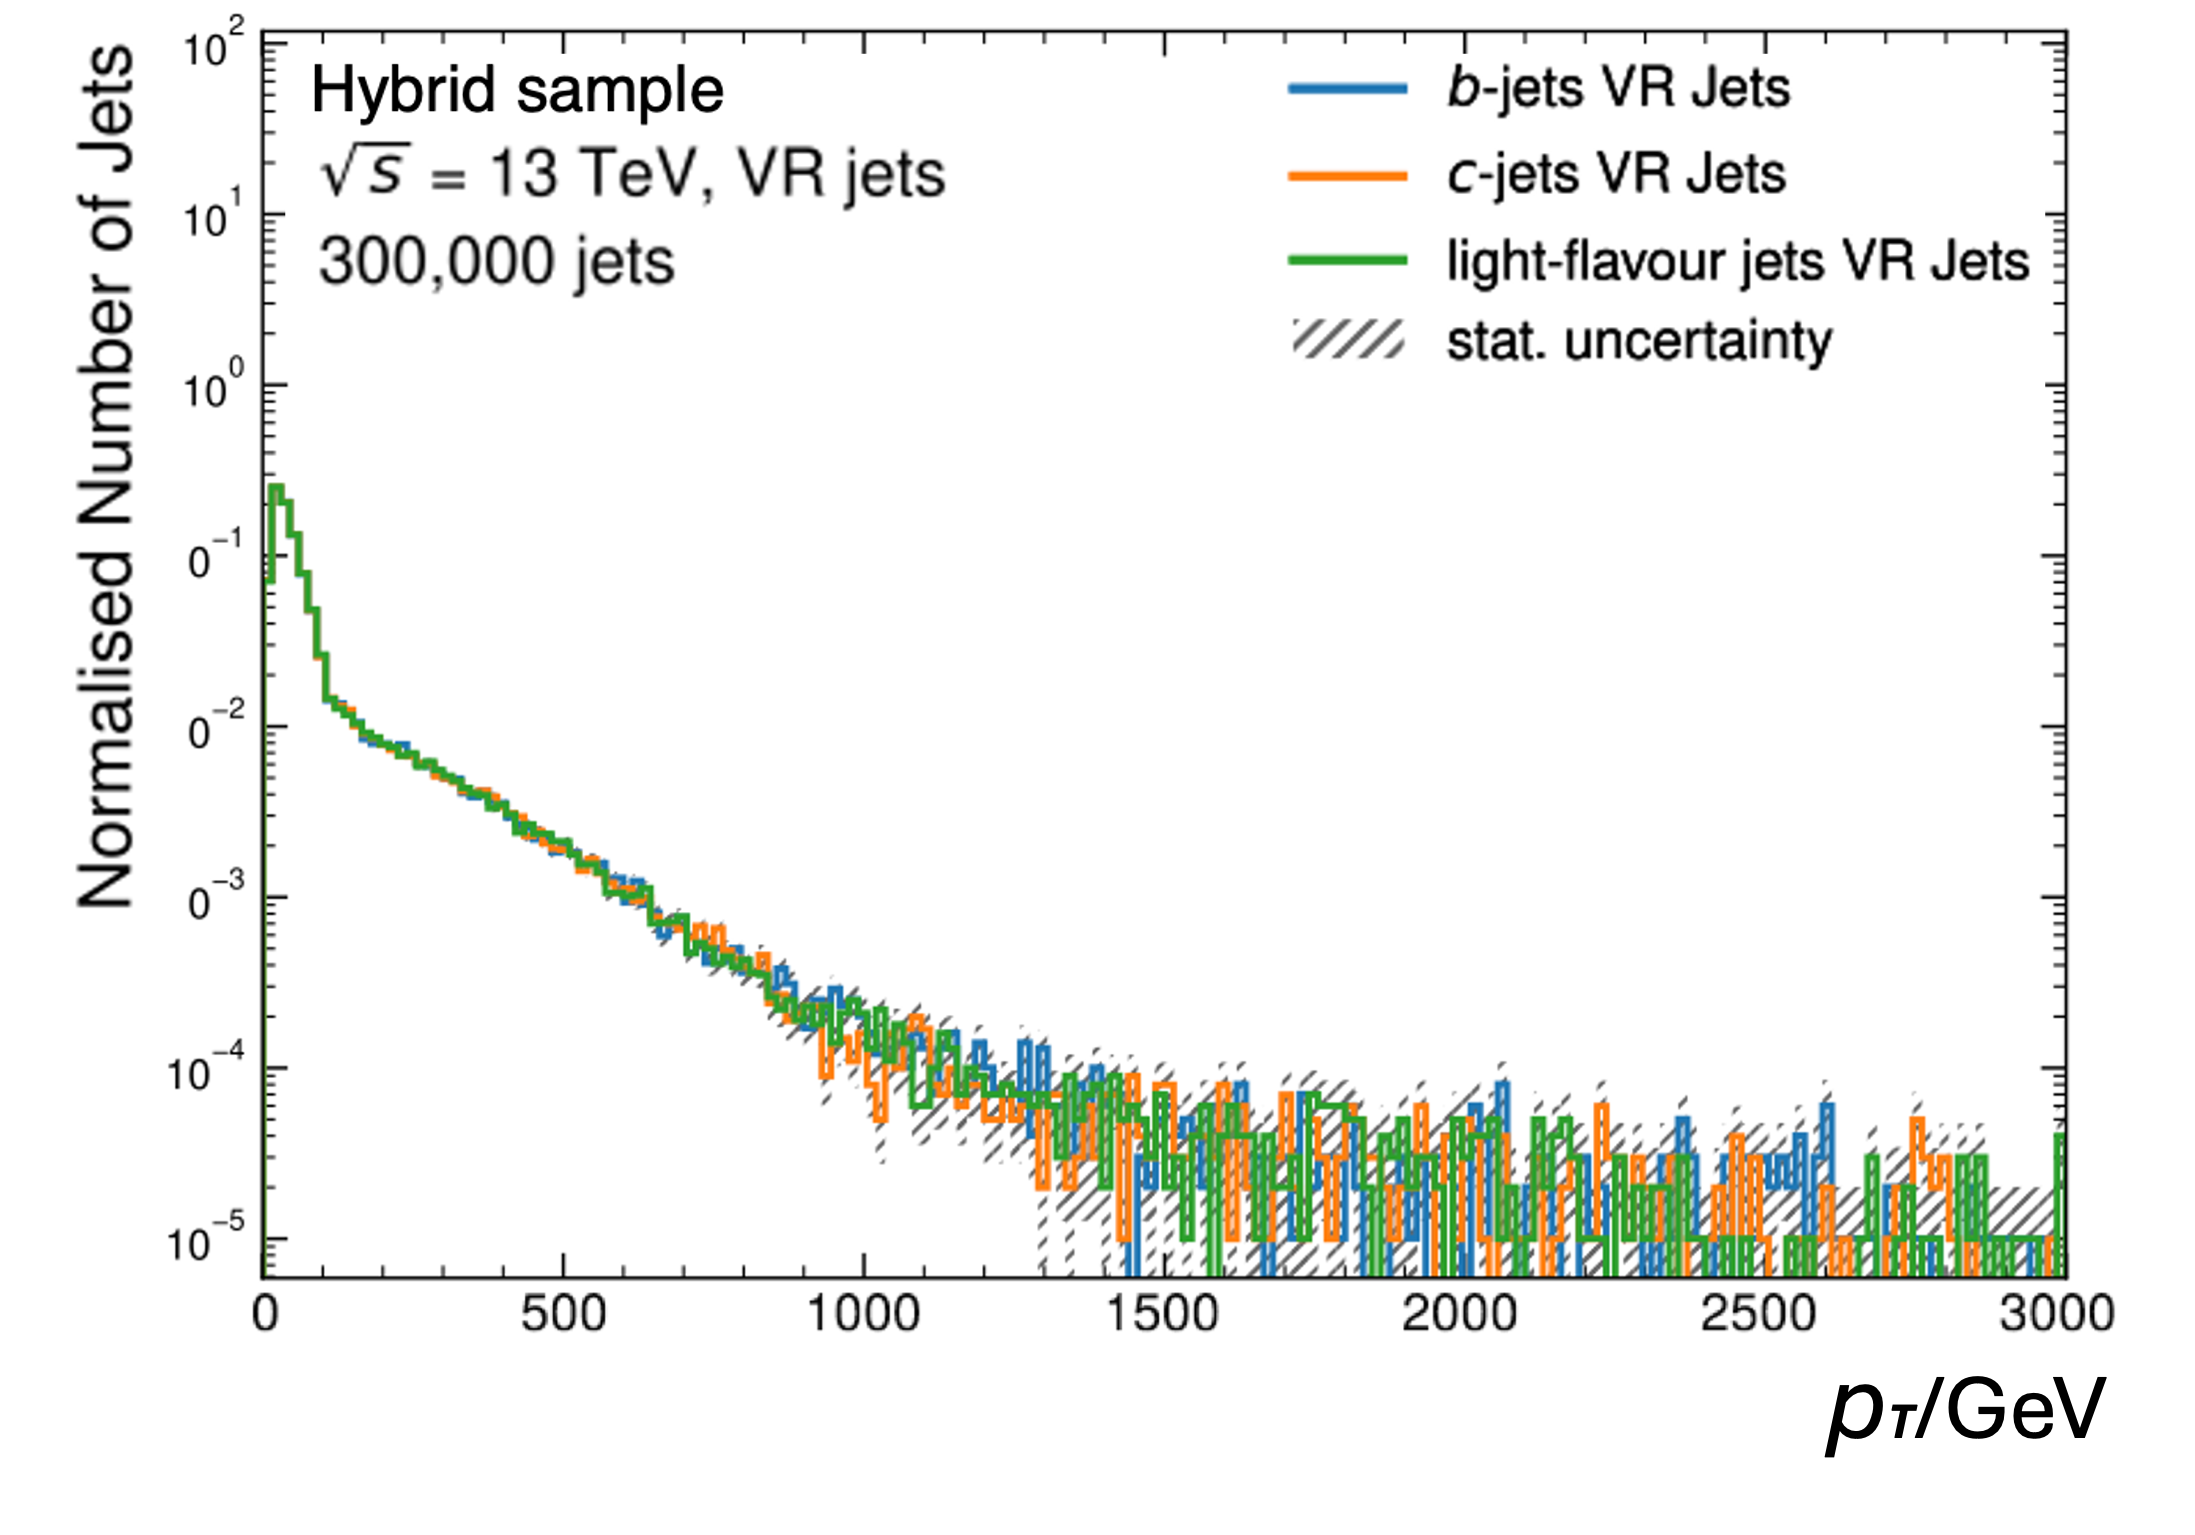
\includegraphics[width=0.48\textwidth]{Images/FTAG/VRDips/JetDist/hspt.png}
      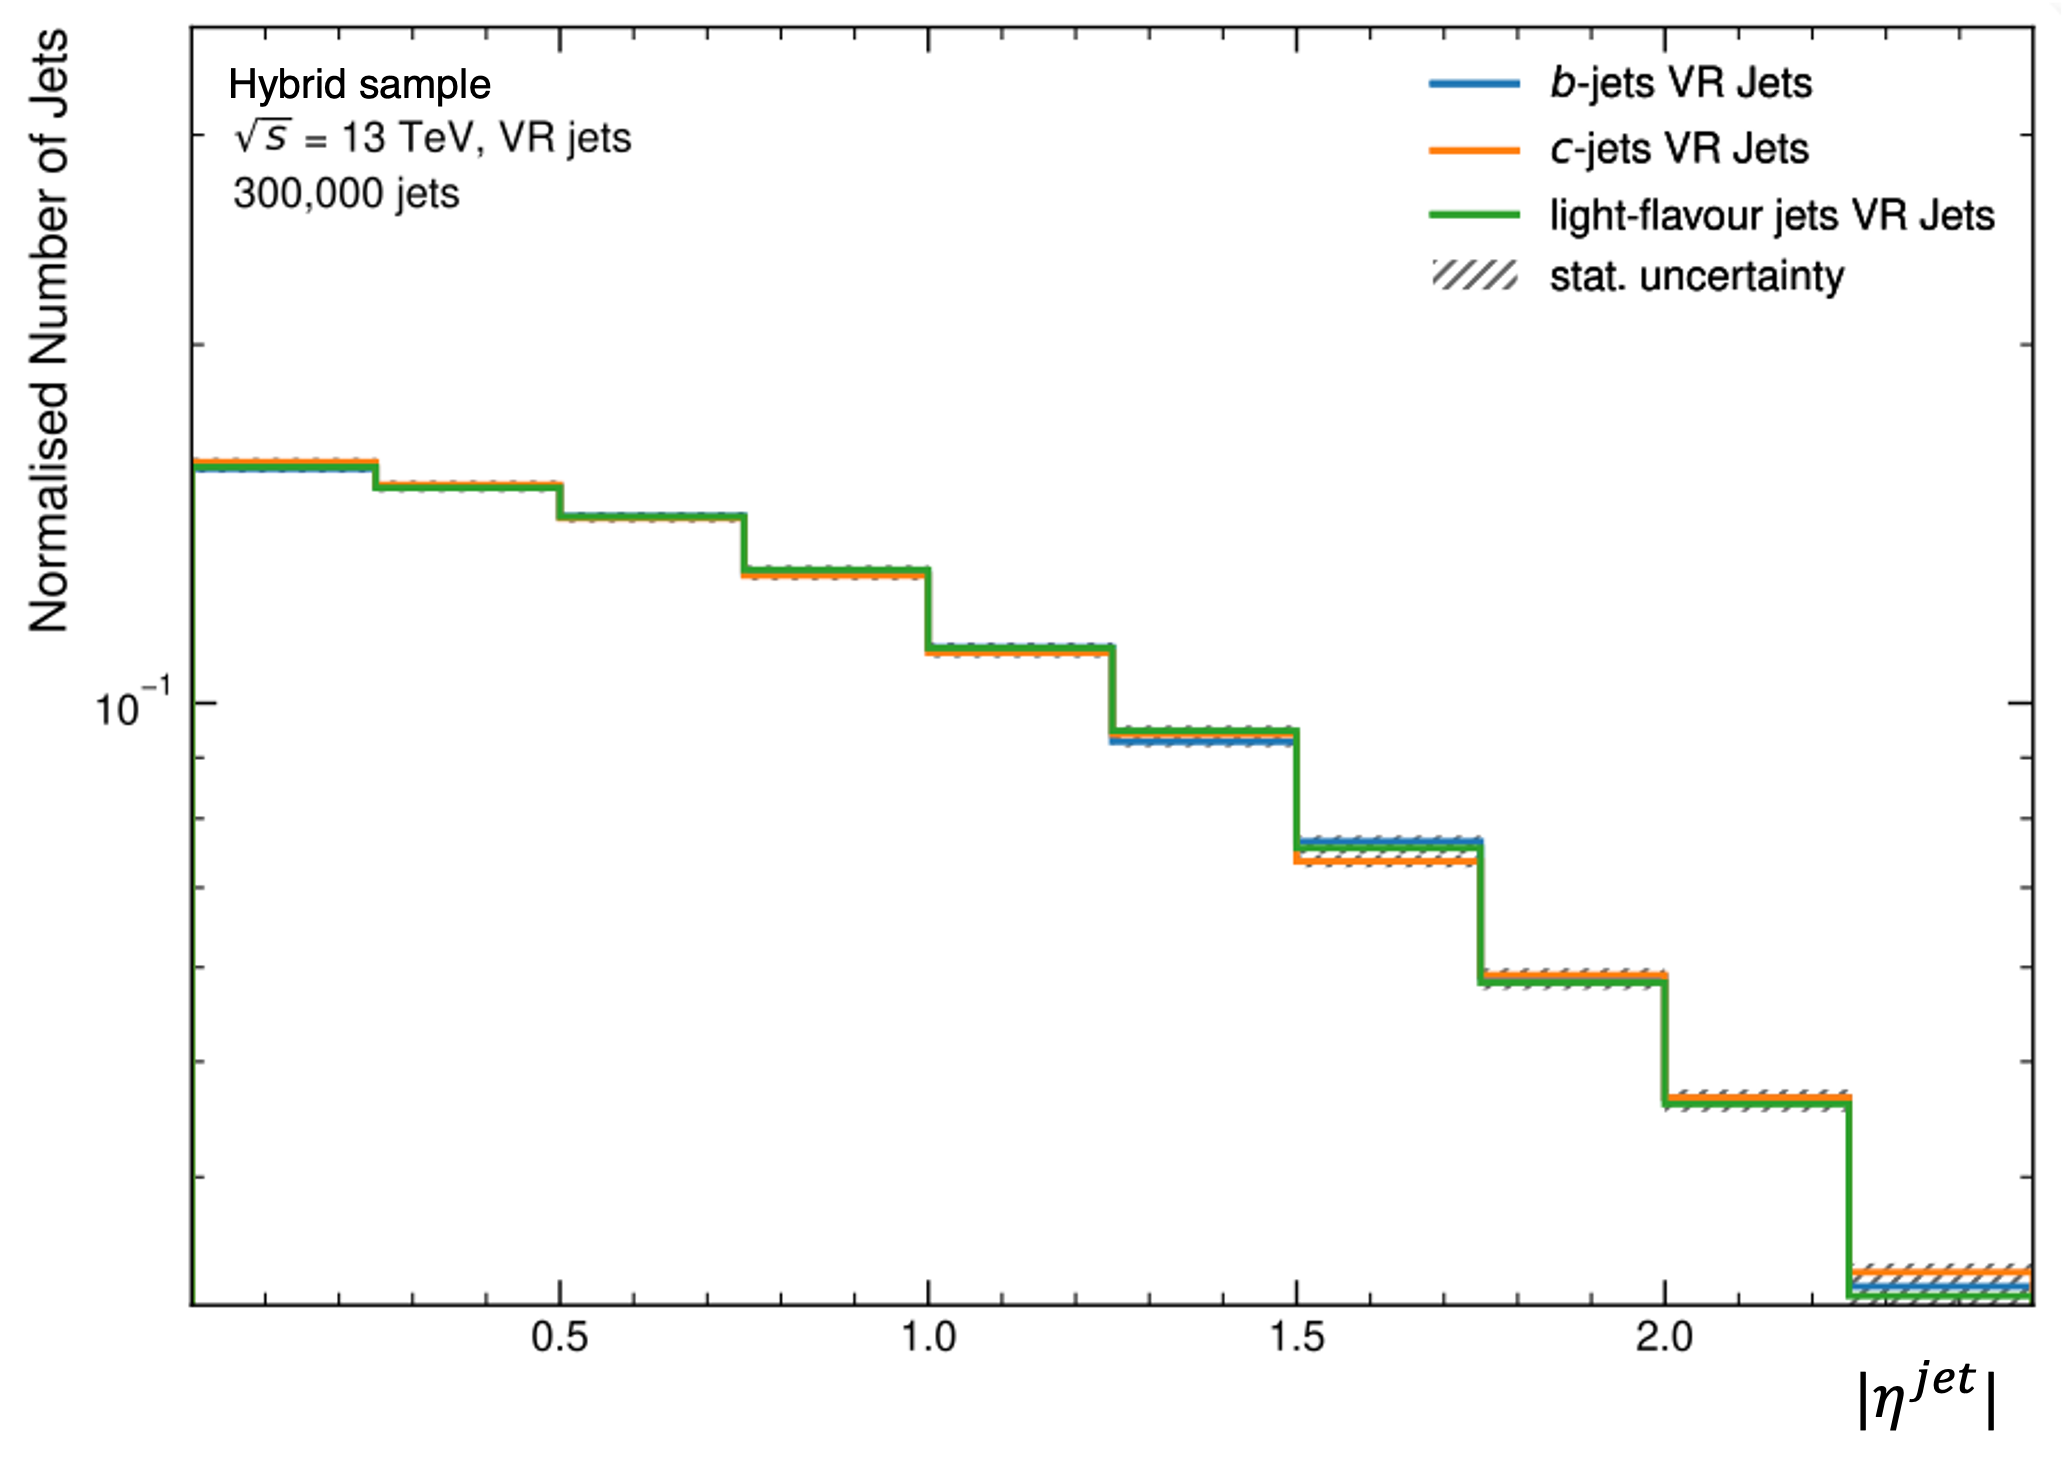
\includegraphics[width=0.48\textwidth]{Images/FTAG/VRDips/JetDist/hseta.png}
      \caption{Hybrid sample.} 
      \label{fig:vrjetdisth}
  \end{subfigure}\\
  \begin{subfigure}[b]{0.98\textwidth}
      \centering
      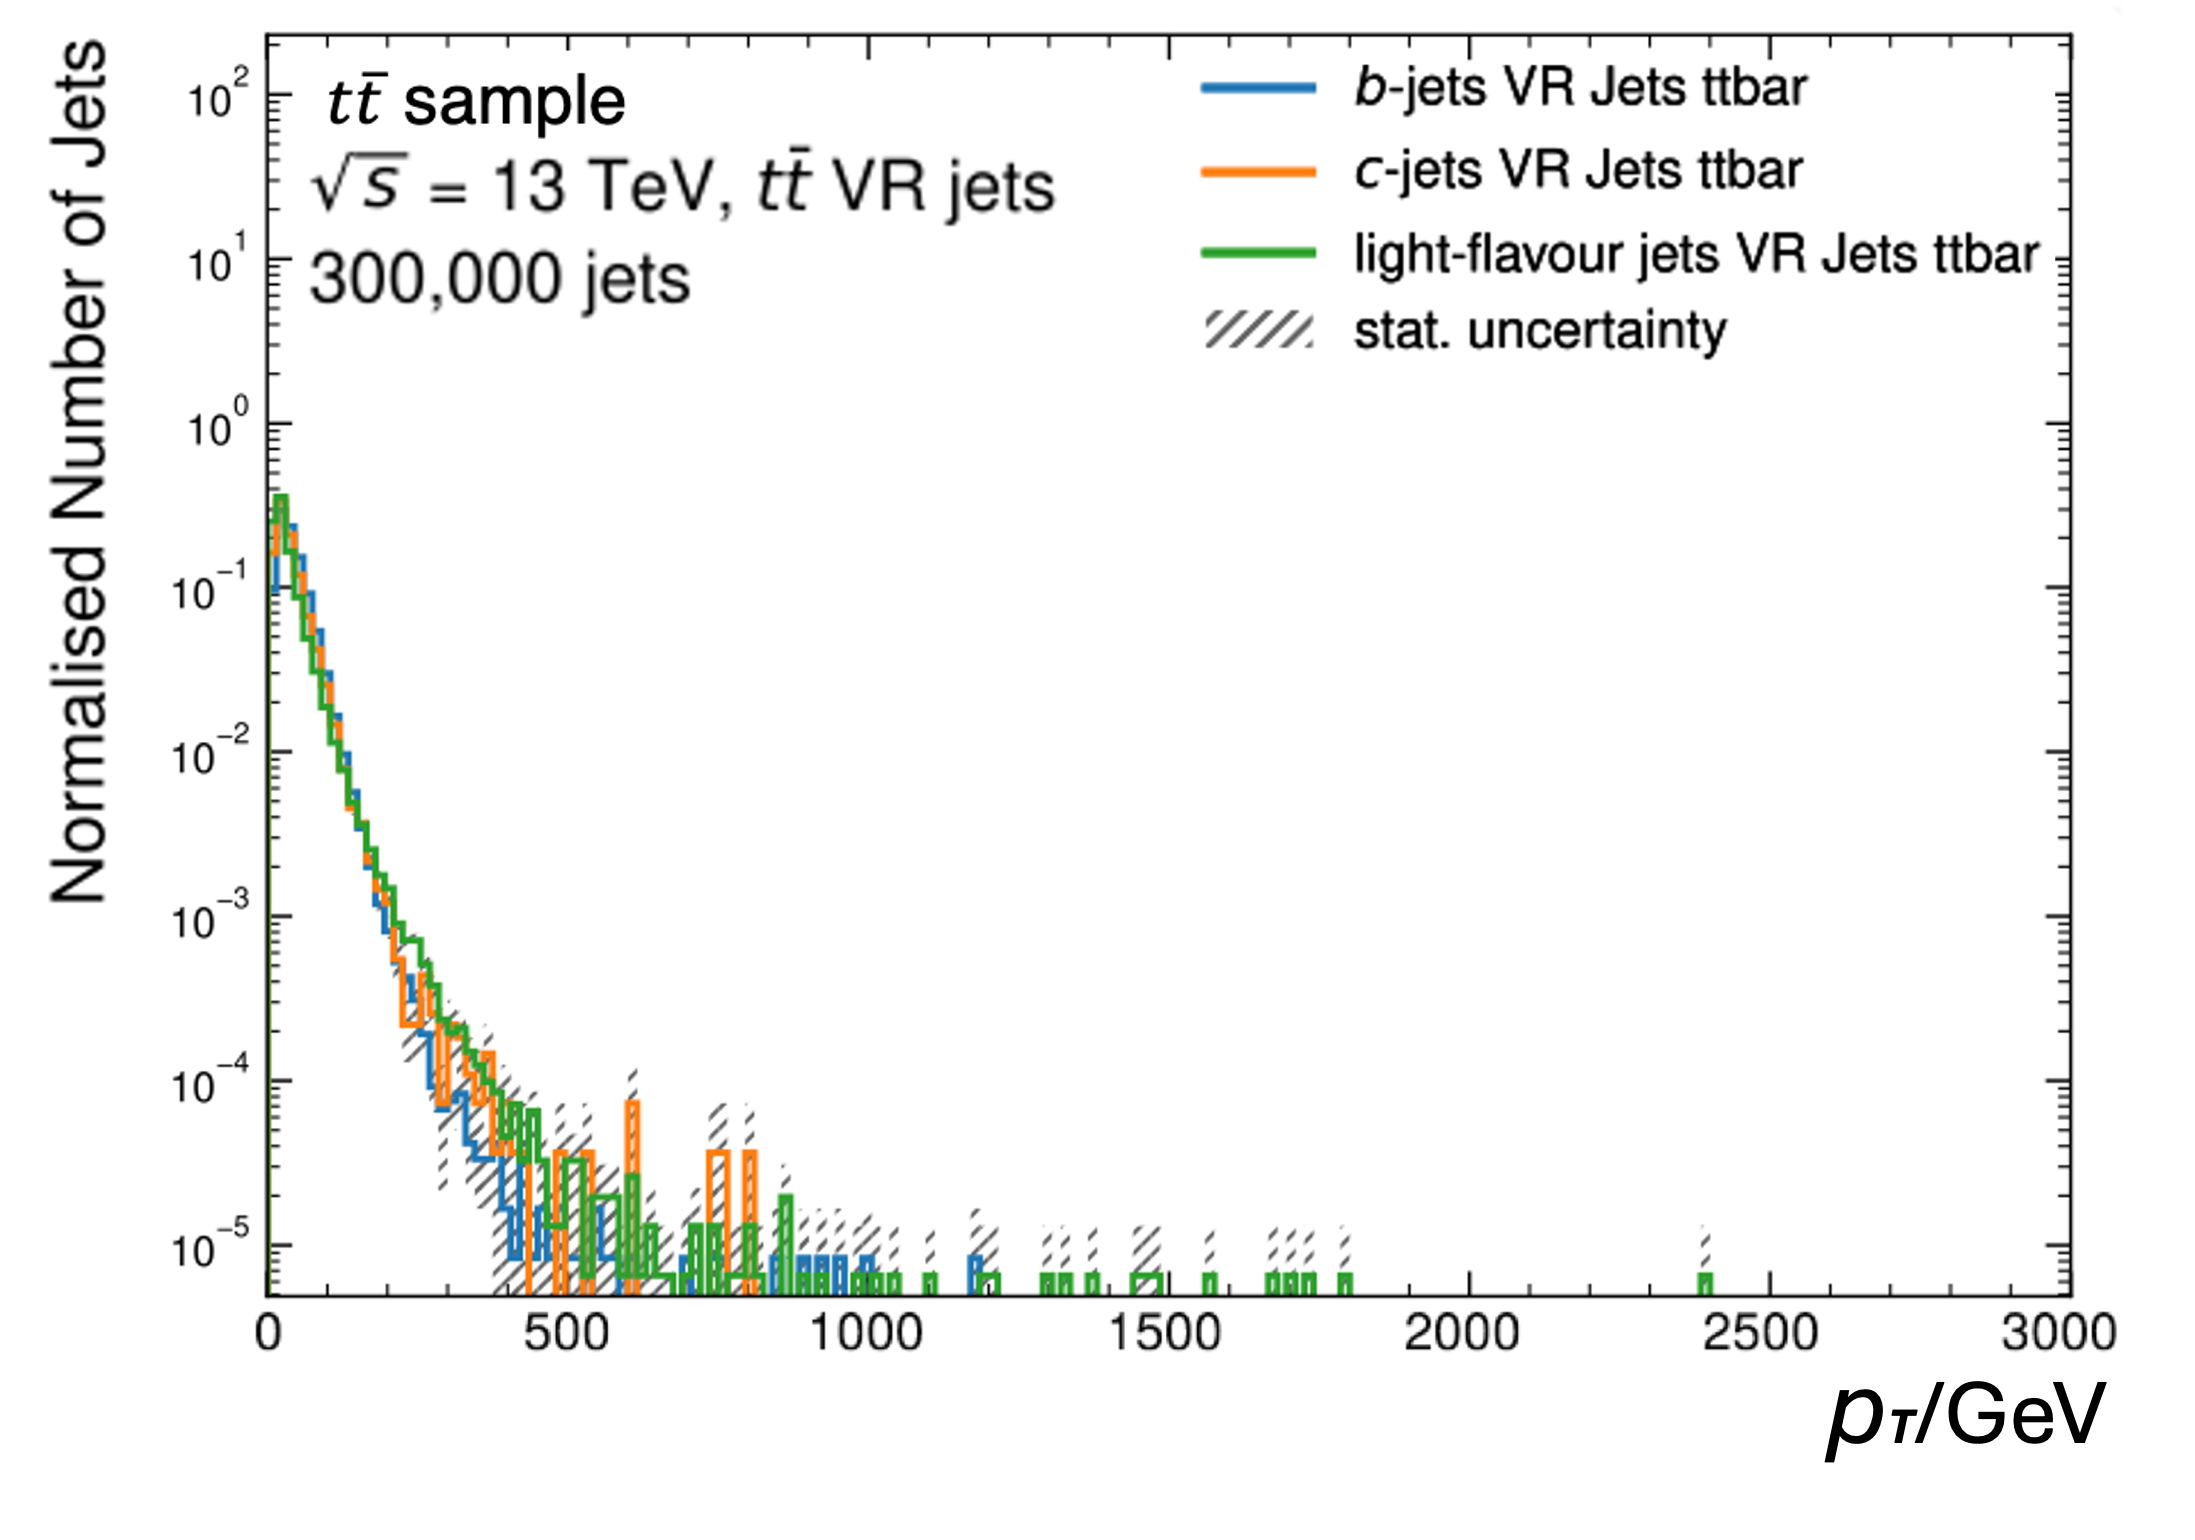
\includegraphics[width=0.48\textwidth]{Images/FTAG/VRDips/JetDist/ttpt.png}
      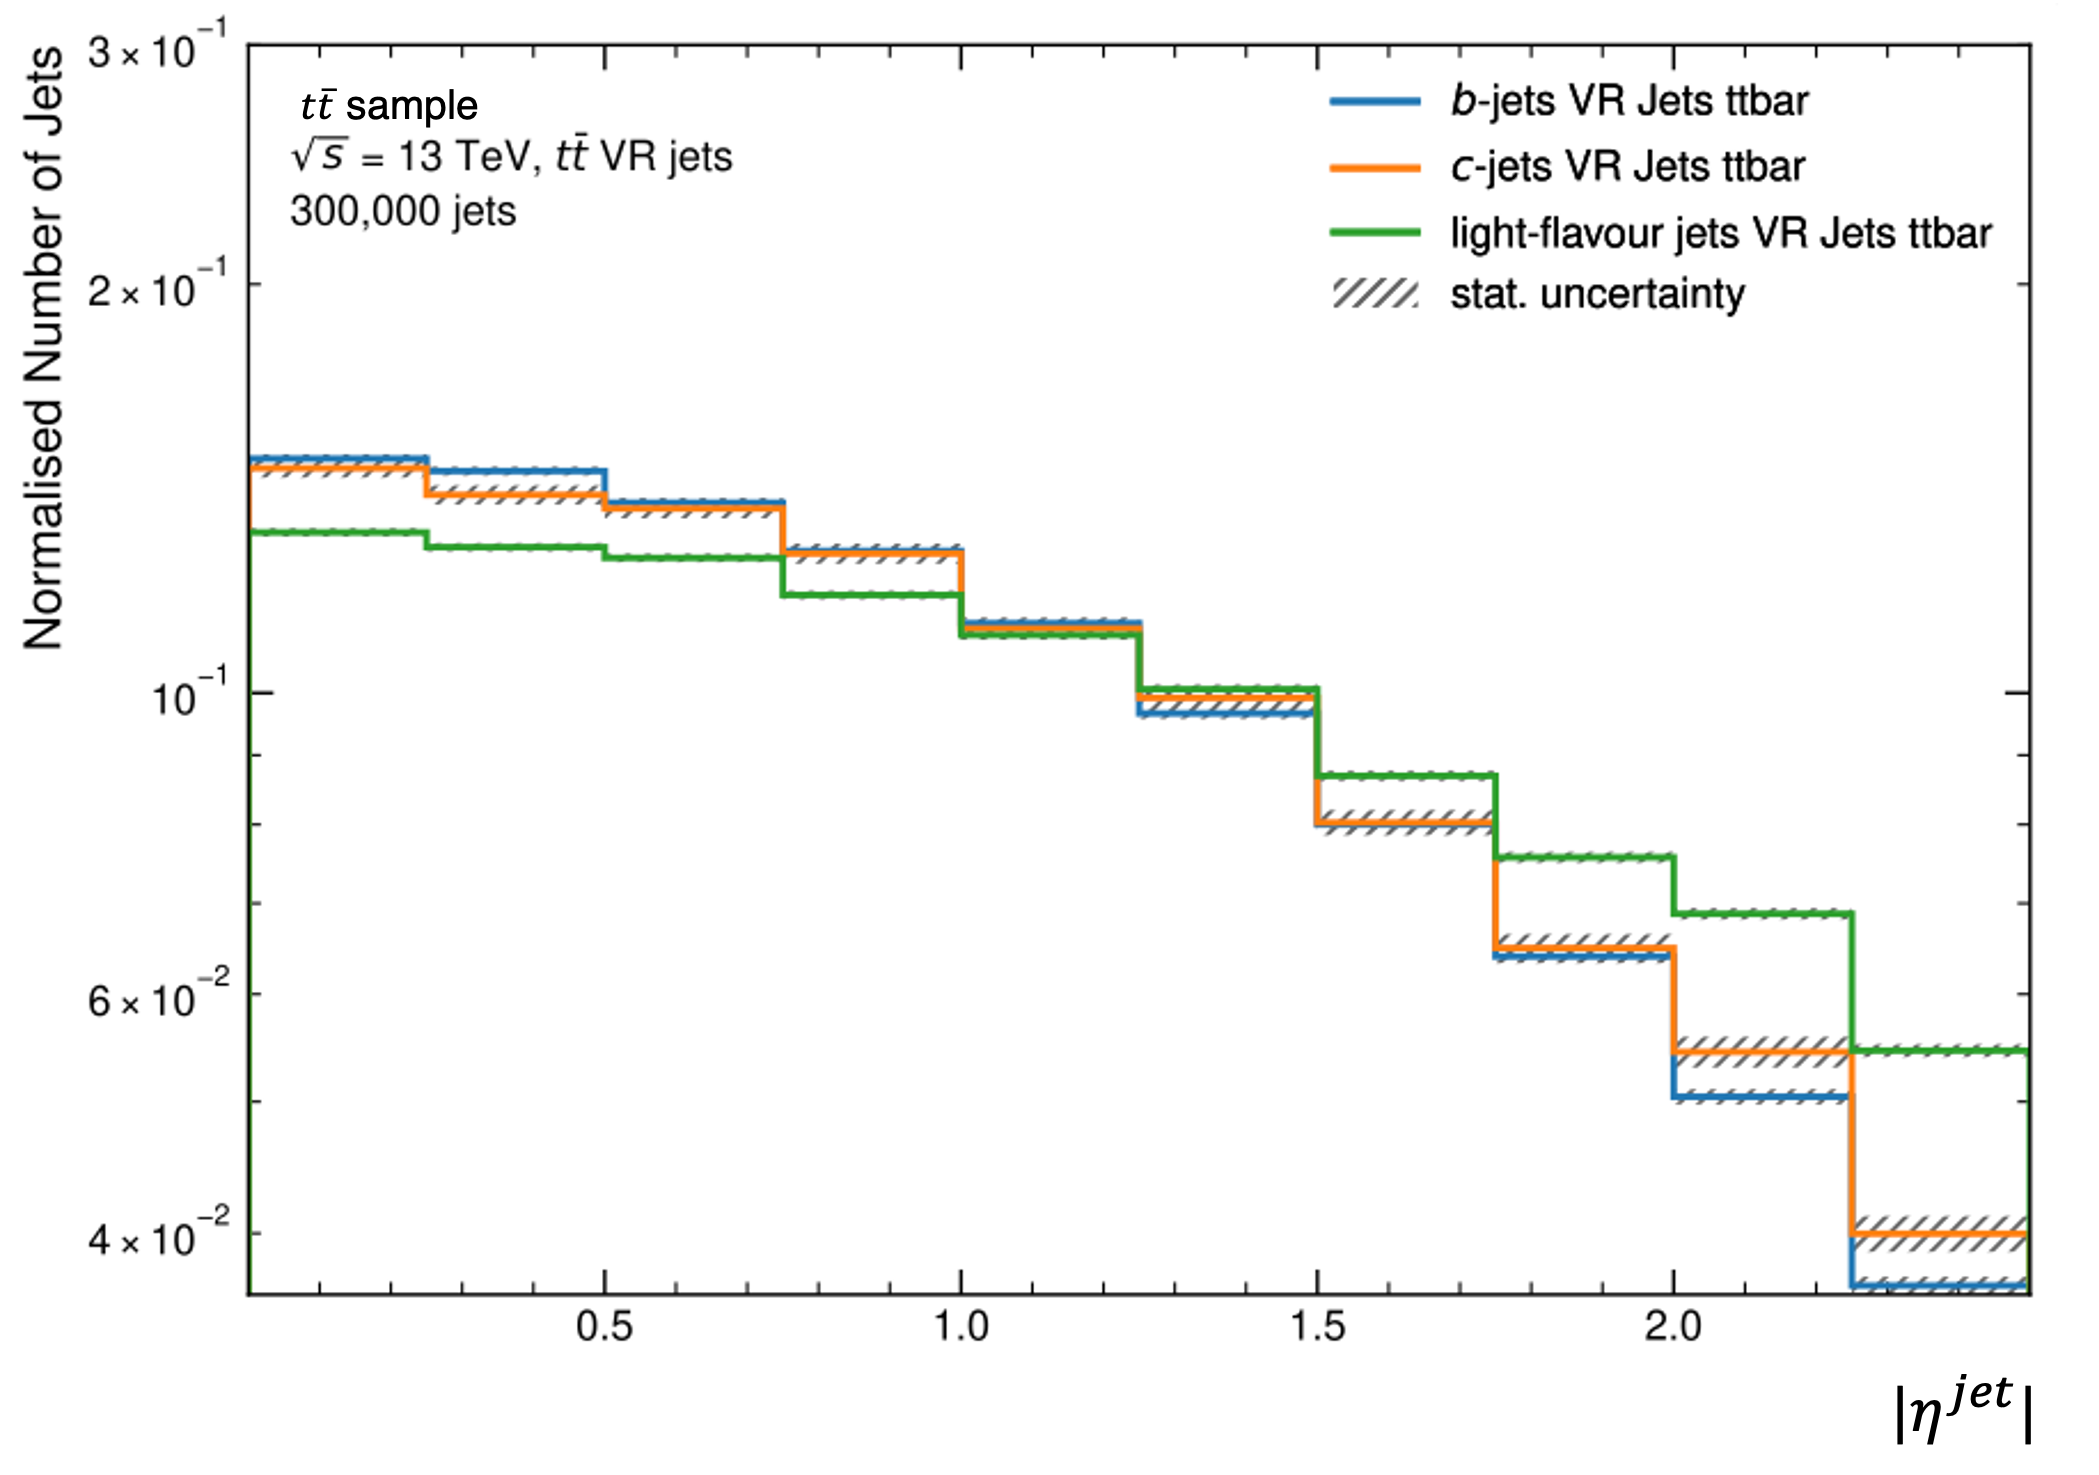
\includegraphics[width=0.48\textwidth]{Images/FTAG/VRDips/JetDist/tteta.png}
      \caption{$t\bar{t}$ sample.} 
      \label{fig:vrjetdistt}
  \end{subfigure}\\
  \begin{subfigure}[b]{0.98\textwidth}
      \centering
      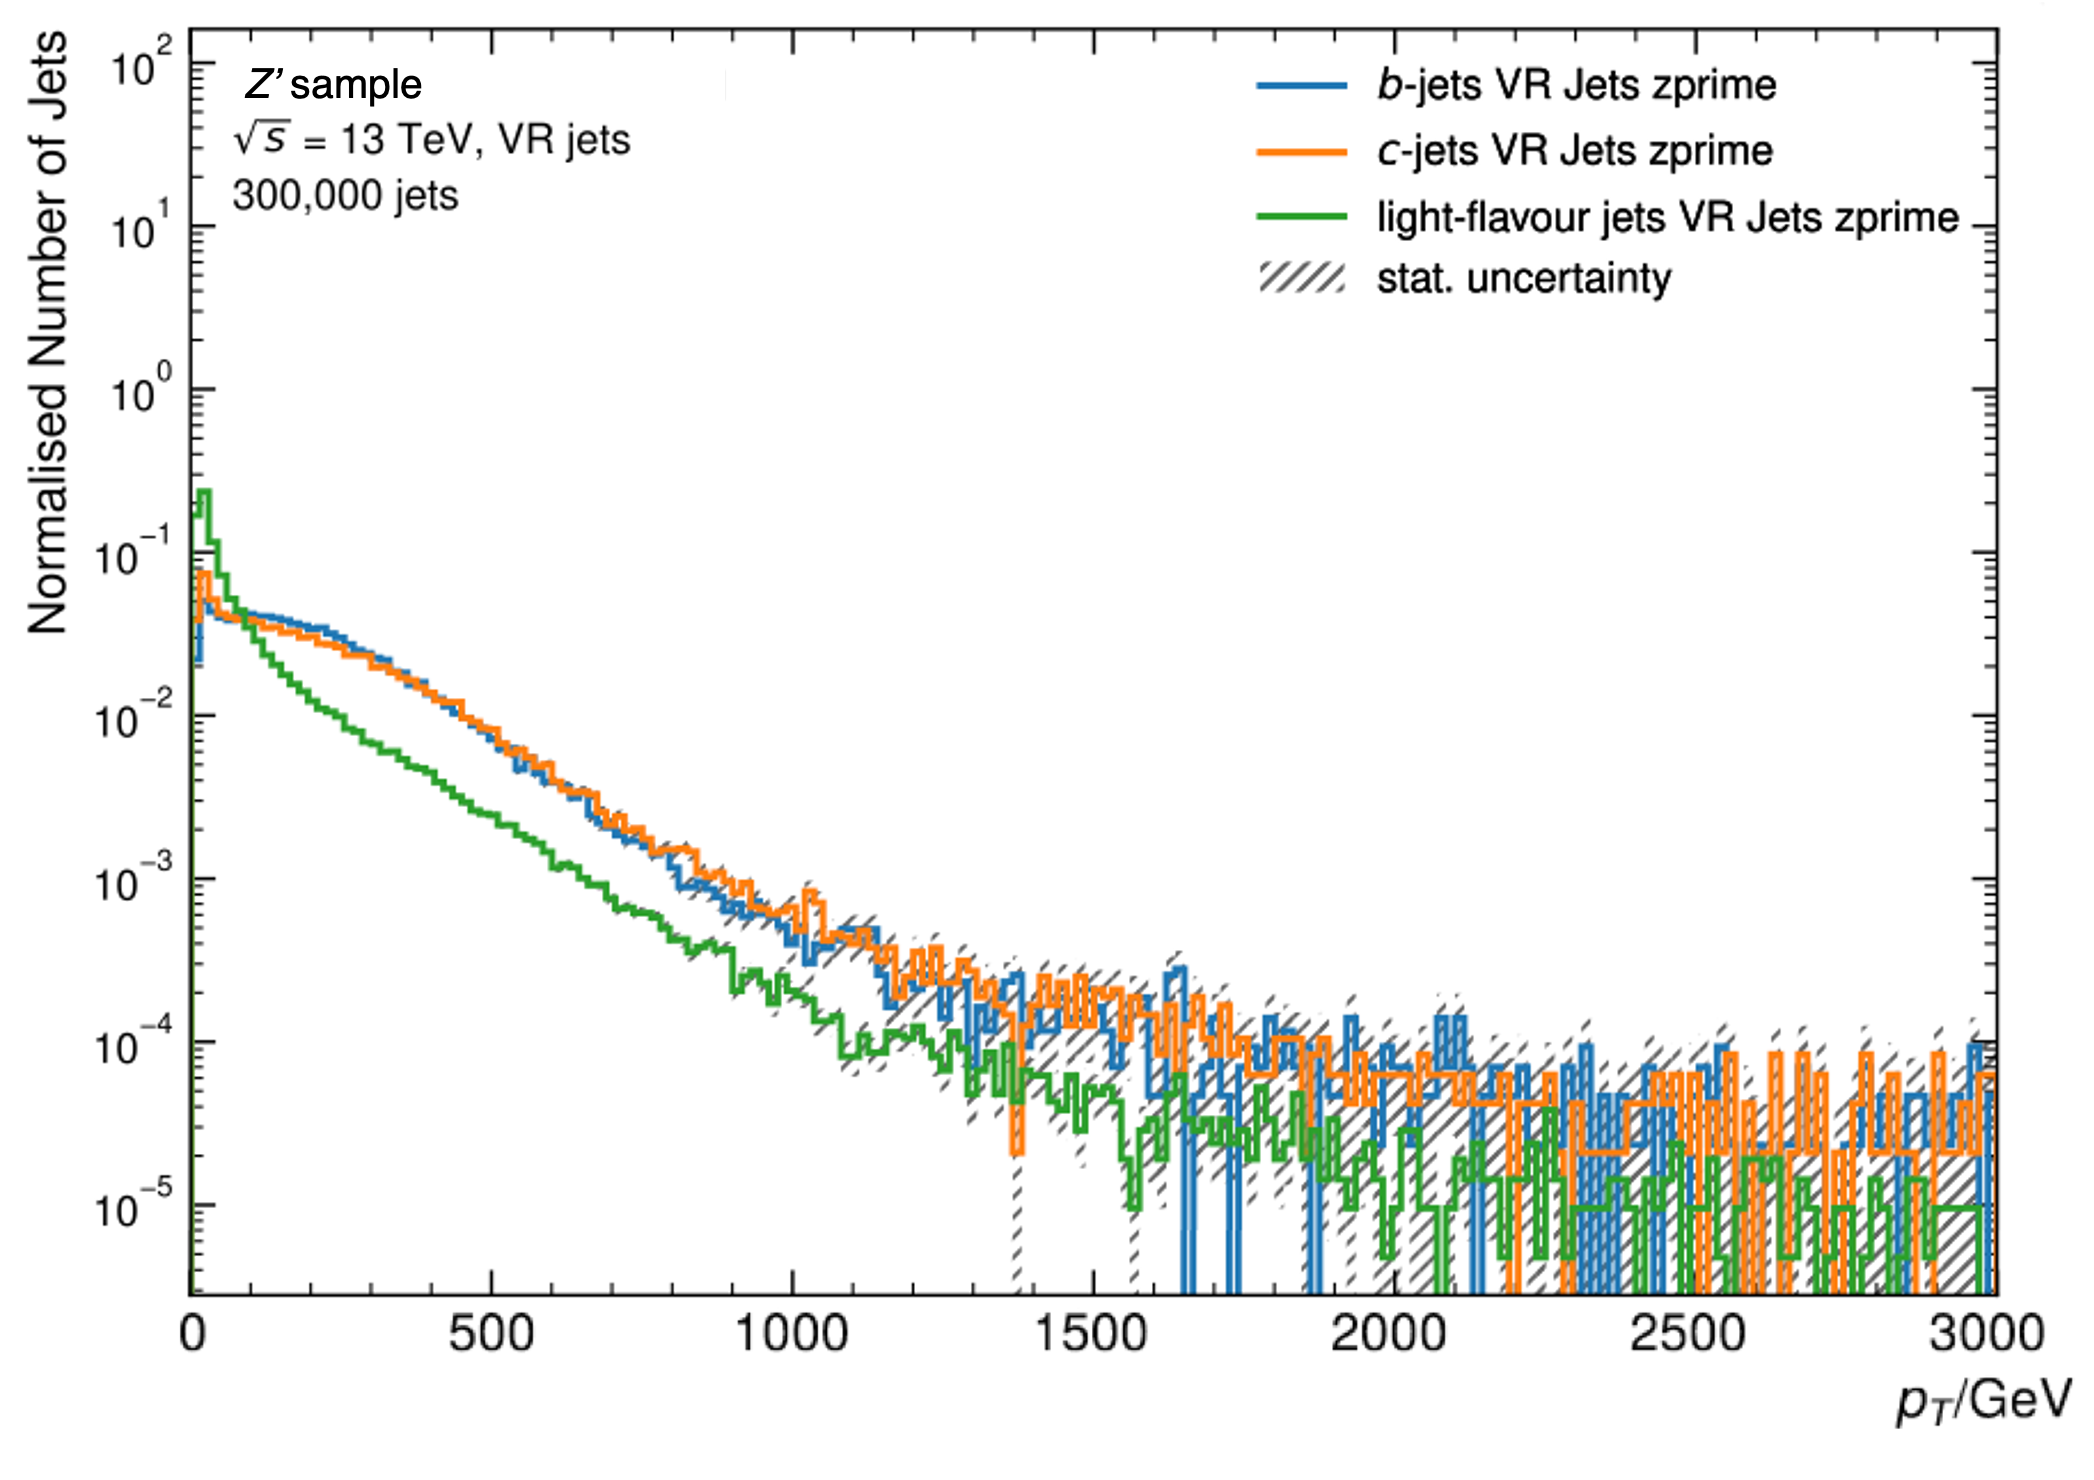
\includegraphics[width=0.48\textwidth]{Images/FTAG/VRDips/JetDist/zppt.png}
      \includegraphics[width=0.48\textwidth]{Images/FTAG/VRDips/JetDist/zpeta.png}
      \caption{$Z'$ sample.} 
      \label{fig:vrjetdiszp}
  \end{subfigure}\\
  \begin{subfigure}[b]{0.98\textwidth}
      \centering
      \includegraphics[width=0.48\textwidth]{Images/FTAG/VRDips/JetDist/grpt.png}
      \includegraphics[width=0.48\textwidth]{Images/FTAG/VRDips/JetDist/greta.png}
      \caption{Graviton sample.} 
      \label{fig:vrjetdisgr}
  \end{subfigure}
  \caption{Distributions for the \gls{vr}-jet training of jets $p_T$ (left) and $|\eta|$ (right) for the hybrid combined process (top row) made from the three bottom processes, in the order $t\bar{t}$, $Z'$, and the graviton.}
  \label{fig:vrjetdist}
\end{figure} 
 
The optimised \gls{dips} model with 62,167 learnable parameters from the previous section was trained for 200 epochs on 4 Quadro RTX 8000 \gls{gpu}. The learning rate started at 0.001 and was reduced by a factor 0.8 on plateaus of 3 epochs, with a batch size of 15k jets, batch normalisation, and a dropout rate of 0.1 for the $F$ network. Training proved stable with no signs of overtraining. The model at the epoch giving the smallest loss on a heldout validation set of 300k jets as well as the best light- and $c$-rejections at a fixed 77\% $b$-tagging efficiency was selected for further comparison. Figure \ref{fig:dipsVRROC} shows the \gls{roc} curves for $b$- and $c$-tagging of the best \gls{dips} model on \gls{vr}-jets (blue), as well as some comparison to the \gls{dips} model trained on PFlow jets (orange) and \gls{rnnip} trained on \gls{vr}-jets from the previous software release R21 (green). 

\begin{sidewaysfigure}
  \vspace{0.5cm}
  %\hspace{0.5cm}
  \begin{subfigure}[t]{0.3\textwidth}
    \centering
    \includegraphics[scale=0.43]{Images/FTAG/VRDips/ROC/ttb.png}
    \caption{$t\bar{t}$ test sample $b$-tagging.}
    \label{fig:dipsVRROCtt}
  \end{subfigure}
  \hfill
  \begin{subfigure}[t]{0.3\textwidth}
    \centering
    \includegraphics[scale=0.43]{Images/FTAG/VRDips/ROC/zpb.png}
    \caption{$Z'$ test sample $b$-tagging.}
    \label{fig:dipsVRROCzp}
  \end{subfigure}
  \hfill
  \begin{subfigure}[t]{0.3\textwidth}
    \centering
    \includegraphics[scale=0.43]{Images/FTAG/VRDips/ROC/grb.png}
    \caption{Graviton test sample $b$-tagging.}
    \label{fig:dipsVRROCgr}
  \end{subfigure} \\
  \begin{subfigure}[t]{0.3\textwidth}
    \centering
    \includegraphics[scale=0.43]{Images/FTAG/VRDips/ROC/ttc.png}
    \caption{$t\bar{t}$ test sample $c$-tagging.}
    \label{fig:dipsVRROCttc}
  \end{subfigure}
  \hfill
  \begin{subfigure}[t]{0.3\textwidth}
    \centering
    \includegraphics[scale=0.43]{Images/FTAG/VRDips/ROC/zpc.png}
    \caption{$Z'$ test sample $c$-tagging.}
    \label{fig:dipsVRROCzpc}
  \end{subfigure}
  \hfill
  \begin{subfigure}[t]{0.3\textwidth}
    \centering
    \includegraphics[scale=0.43]{Images/FTAG/VRDips/ROC/grc.png}
    \caption{Graviton test sample $c$-tagging.}
    \label{fig:dipsVRROCgrc}
  \end{subfigure}
  \caption{\gls{roc} curves for $b$-tagging (top) and $c$-tagging (bottom) on test samples of 300 k jets for $t\bar{t}$ (left), $Z'$ (centre), and the graviton process (right). Models are displayed as curves of different colours, with the \gls{vr}-jets \gls{dips} in blue, the \gls{dips} model trained on PFlow jets in orange, and \gls{rnnip} trained on \gls{vr}-jets from the previous software release R21 in green.}
  \label{fig:dipsVRROC}
\end{sidewaysfigure}

Training \gls{dips} on a dedicated set of \gls{vr}-jets clearly improves performance over relying on the PFlow-trained version, as observed by comparing the blue (\gls{vr}-trained \gls{dips}) to orange curves (PFlow-trained \gls{dips}). At a $b$-tagging efficiency of 77\%, the light-rejection is PFlow-trained \gls{dips} is indeed roughly 40\% lower. However, the $c$-rejection does not benefit as much, being either on par or even lower for the \gls{vr}-trained \gls{dips} on the $t\bar{t}$ samples. This difference in performance indicates an inappropriate choice of $f_c$ value for the $b$-tagging discriminant of the \gls{vr}-trained \gls{dips}. A so-called \textit{flavour fraction scans}, displaying the rejections at a fixed tagging efficiency for different value of the flavour fraction, can lead to a better choice for a balanced improvement in both background jet rejections. However, \gls{dips} probabilities are not meant to be used directly as discrimant but rather passed on to the high level algorithm \gls{dl1d}, hence this optimisation is reserved for the final model as presented in Chapter \ref{sec:VRdl1dTrain}. Figures \ref{fig:dipsVRROCttc} to \ref{fig:dipsVRROCgrc} lead to similar conclusions for $c$-tagging.

\subsection{Training of DL1d \& DL1r with PFlow for Run 3}
The ATLAS Collaboration continuously updates its software, updating specific methods to adopt new techniques, maintaining its many tools and adding capabilities. In preparation for the current Run 3 of the \gls{lhc} that started in 2022, ATLAS improved its reconstruction software from release 21 (R21) to release 22 (R22). As such, important elements used by flavour tagging methods have changed, requiring to retrain all taggers to ensure optimal performance under the new conditions. This work presents the first ATLAS study of the retraining of \gls{dl1r} on the new release R22 and the first training of \gls{dl1d}, including the \gls{dips} sub-tagger in the high-level flavour tagging tool. Other important novelties of this work are the possible inclusion of $\tau$-jets in the \gls{dl1} model's predictions and a new technique to efficiently process the training data into high statistics dataset using importance sampling, as mentioned in the previous section. The interest of including $\tau$ stems from their tendency to be miss-classified as $c$-jets when hadronically decaying, as both particles commonly leave three particles in the detector. The resulting taggers are observed to efficiently identify $\tau$-jets thereby providing a new way to perform $\tau$-identification and improving $c$-jet tagging. However, due to the widespread use of the \gls{ftag} algorithms and the difficulties arising in calibrating a tagger with excellent rejection against $\tau$-jets, these are not included in the default version of the tagger nor in the results shown here, but are actively under study for the new generation of tagger in the GN family. \\ % Problem: reference to tau tagging but no plots ... add them?
Two samples, the $t\bar{t}$ and $Z'$ from proton-proton collisions at $\sqrt{s} = 13$, are simulated and combined in the datasets, as described in Section \ref{ftagdatasets}. For both samples, PFlow jets are reconstructed using the anti-$k_T$ algorithm with radius $R = 0.4$. These two samples are combined into a single \textit{hybrid} sample to train the taggers, with 70\% of the total number of jets coming from $t\bar{t}$ and the remaining from the $Z'$. The $t\bar{t}$ and $Z'$ samples cover, respectively, a low- and high-$p_T$ region based on a reconstructed $b$-hadron $p_T$ separation threshold of 250 GeV for $b$-jets and a jet $p_T$ of 250 GeV for non-$b$-jets. They are re-sampled to have the same $p_T-|\eta|$ distributions, as described in the next paragraph. The relative proportion of each sample was chosen to avoid any discontinuity in the $p_T$ spectrum at their junction, as evidenced in Figure \ref{fig:distTraining}. The final evaluation of the performance of a trained tagger is performed on separated test sets of both processes and unfolded over the flavours.\\

\begin{figure}[h!]
  \center
  \includegraphics[width=0.48\textwidth]{Images/FTAG/DL1d/ptdist.png}
  \includegraphics[width=0.48\textwidth]{Images/FTAG/DL1d/etadist.png}
  \caption{The $p_T$ (left - in MeV) and $|\eta|$ distributions of the resampled $b$-, $c$-, and light-jets in, respectively, blue, orange, and green. The three ses are resampled to have the same $p_T-|\eta|$ 2D distributions. The flat $p_T$ spectrum extending up to several TeV is due to the exotic $Z'$ process generated with varying mass, starting at 150 GeV. The large peak at lower $p_T$ is the $t\bar{t}$-process. These sets have 8.3 million jets per flavour.} 
  \label{fig:distTraining}
\end{figure}

ATLAS flavour tagging tools are widely used across the Collaboration. It is therefore essential for the taggers not to learn specific features of the processes simulated but to focus on the inherent differences between the studied flavours in order to generalise to other processes. An effective way to limit the importance of the simulated processes is to downsample the hybrid sample in [$p_T - \eta$] bins to have the same number of $b$-, $c$-, and light-jets in each 2D bin. This removes the distinction of kinematic phase space between each flavour due to the process specific physics. To avoid biasing the output of the tagger towards the most likely flavours in the process, each jet-flavour is also required to be equally likely in the training set, a requirement satisfied by having the same yield of $b$-, $c$-, and light-jets. Applying this technique, the total statistics available for the R22 training is of $25 \times 10^{6}$ jets per flavour for training. The $t\bar{t}$ and $Z'$ samples for validation and testing are each made of 1 million jets and are not downsampled to have the same [$p_T - \eta$] distribution nor the same yield of different flavours: they represent a realistic distribution of the underlying processes. The main limitator when downsampling are $c$-jets, as all $c$-jets from the $t\bar{t}$ process are selected which limits the amount of $b$- and light-jet that can be taken. This process is extremely wasteful, using only 17\% (11\%) of all available $b$-jets (light-jets) in the $t\bar{t}$ sample.\\

Training is done with the \uppercase{Umami} framework \cite{UmamiCite} based on TensorFlow \cite{tensorflow2015-whitepaper} for 300 epochs with a variable learning rate schedule and the default network structure adopted in the previously released \gls{dl1r} (R21): 8 fully connected \gls{nn} of smoothly-decreasing sizes in [256, 128, 60, 48, 36, 24, 12, 6] with \gls{relu} activation leading to a final softmax layer producing the predicted probabilities for each flavour. While the \gls{dips} probabilities used as inputs to \gls{dl1d} come from a model trained on the new release, the \gls{rnnip} probabilities are still from a model trained on the previous one (R21) \cite{ATL-PHYS-PUB-2017-003, ATL-PHYS-PUB-2020-014}. Indeed, due to its significantly lower performance, \gls{rnnip} is no longer supported in the new release and is included for sake of comparability to the previous techniques. The models at an epoch offering the best combined results in terms of $b$-tagging efficiency and rejection from $b$-jets on the validation set are selected for further analysis. Importantly, every training converged to a fixed set of performance values, with no overtraining occurring.\\

Several modifications to the model architecture, list of input variables, and preprocessing and training procedures have been explored, with no significant gain observed:
\begin{itemize}
\item The preprocessing steps were revised to reduce the size of the evaluation sets for the benefit of the training one. A dual approach, downsampling light-jets and upsampling $c$-jets to the $b$-jets [$p_T - \eta$], has also been implemented. As previously described, this approach uses importance sampling with replacement to obtain the same fraction of the different flavours and the same $p_T$ and $|\eta|$ distribution. While the performance of the majority classes was observed to improve, the efficiency at tagging the upsampled minority class ($c$-jets) was slightly lower. This trade-off can be compensated by modifying the flavour fractions and thus does not result in any significant performance changed. This is likely due to the model saturating its performance given the large dataset already available. Other models, such as those from the GN family that have more parameters, have however been observed to make gains from the importance sampling approach.
\item Several modifications to the list of input features have been attempted, with no clear advantage uncovered. Adding pile-up information (the actual number of interactions per crossing and the number of primary vertices were tested) was not observed to have an impact on the tagging efficiency. Adding other variables from \gls{sv1} or JetFitter was also not observed to improve performance. However, a positive observation is that the IP2D and IP3D taggers can both be safely removed without changes to the performance, as the information they add is in all likelihood now covered by the \gls{dips} sub-tagger, thereby reducing the list of sub-taggers to maintain and simplifying the architecture.
\item The structure of the network and its training procedure, leveraging transfer learning. Using samples produced with an older release of the ATLAS software (R21) to pre-train the model was not observed to deliver a boost in performance when later training on the new release (R22). Changing the size of the network and the batch size was also not observed to have a positive effect.
\end{itemize}

The conclusion driven by the lack of improvements from these three attempts is that models built on this simple \gls{dnn} structure with large dataset are already likely saturating their performance from the set of inputs. The performance of the retrained \gls{dl1r} tagger on the new release was found to be in good agreement with the at-the-time released \gls{dl1r}, despite using the same training of \gls{rnnip} on the previous release. In order to establish a meaningful benchmark for the newly trained taggers, the performance of the then released \gls{dl1r} tagger, trained and evaluated on an analogous set of samples from the previous release (R21), is included in the following results as benchmark under the label \textit{Recom. \gls{dl1r}}. A first look at the new family of taggers is also advertised by plotting the performance of a pre-release \gls{gn1} tagger, although this is discussed in further details in the next Chapter \ref{chap:GN}. \\

Figure \ref{fig:DL1dtt} presents the \gls{roc} curves on the $t\bar{t}$ (left) and $Z'$ (right) samples for $b$-tagging. These \gls{roc} plots show, on the $x$-axis, the $b$-tagging efficiency ($\epsilon^b_b$) versus, on the $y$-axis, the rejection $\mathcal{R}^b_Y$ for $Y \in$ [$c$, light]. The two bottom sub-plots present the ratio of the c-jet rejection and light-jet rejection curves to the blue ones. This blue curve is the recommended \gls{dl1r} performance and serves as the baseline of the comparison, while the new tagger \gls{dl1d} is plotted in orange. Figure \ref{fig:DL1dz} shows the same plots for $c$-tagging, with respect to $b$- and light-jet rejections. The important observation is the clear gain obtained when replacing \gls{rnnip} with \gls{dips}. Both the $b$- and $c$-tagging performance of \gls{dl1d} clearly dominate the \gls{dl1r} versions, with a significant improvement in background flavour rejection for all tagging efficiency considered, as summarised in Table \ref{tab:max-perf}. The largest improvement in performance is obtained for $b$-tagging on the $t\bar{t}$ process, corresponding to a lower jet momentum. This latter points to a dynamical behaviour of the \gls{dips} subtagger that can be traced back to the looser jet selection. Higher momentum jets are more likely to have a larger set of tracks and these tracks tend to be closer to each other due to relativistic boosting. The looser selection forces the \gls{dips} model enduce to sift through a larger set of noisy tracks which brings lower performance at higher momentum, while a gain is obtained at lower momentum from the nicer geometrical separation and smaller initial set.  \\

The light-rejection from $b$-jets \gls{roc} curve in Figure \ref{fig:DL1dtt} traces an elbow at high $b$-jet efficiencies. This effect is also present in the $b$-rejection from $c$-tagging, Figure \ref{fig:DL1dz}. Both correspond to a set of, respectively, light-jets and $b$-jets that do not overlap with the $b$-jets $b$-tagging and $c$-jets $c$-tagging discriminants distributions, as shown in Figures \ref{fig:scoreDL1dtt} and \ref{fig:scoreDL1dz}. These ``background`` jets are easily removed from the core set of ``signal'' jets due to inherent differences between the flavours and the discrete nature of some sub-taggers used. \\

The background rejections of the various taggers for $b$-tagging ($c$-tagging) as a function of the jet transverse momentum $p_T$ at an inclusive $b$-efficiency of 70\% ($c$-efficiency of 30\%) per region displayed are shown in Figure \ref{fig:ptDL1dtt} (Figure \ref{fig:ptDL1dz}). Throughout the $p_T$ range considered, \gls{dl1d} outperforms the \gls{dl1r} tagger. The low $p_T$ $b$-rejection from $c$-jets is noticeably better for the newly trained tagger compared to \gls{dl1r}. The discontinuity of the rejections between the two processes arises from the inclusive $b$-tagging efficiency being computed inclusively per-region and not exclusively for the whole range. 

%
\begin{center}
\begin{figure}[h!]
\centerline{
\includegraphics[scale=0.45]{Images/FTAG/DL1d/ROC/ttb.png}
\includegraphics[scale=0.45]{Images/FTAG/DL1d/ROC/zpb.png}
}
\caption{Performance for $b$-tagging with a flavour fraction of $f^b_c = 0.018$. Left: $t\bar{t}$; right: $Z'$. Top: \gls{roc} curves; centre: ratio of $c$-jets rejection from $b$-jets relative to the R22-retrained \gls{dl1r}; bottom: same ratio for light-jets rejection. List of taggers: {\color{blue} recommended \gls{dl1r} from the previous release}; {\color{orange} \gls{dl1d} trained on the new release}; {\color{greenforest} \gls{gn1} test-model trained on the new release}.}
\label{fig:DL1dtt}
\bigskip
\centerline{
\includegraphics[scale=0.45]{Images/FTAG/DL1d/ROC/ttc.png}
\includegraphics[scale=0.45]{Images/FTAG/DL1d/ROC/zpc.png}
}
\caption{Performance for $c$-tagging with a flavour fraction of $f^c_b = 0.2$. Left: $t\bar{t}$; right: $Z'$. Top: \gls{roc} curves; centre: ratio of $b$-jets rejection from $c$-jets relative to the R22-retrained \gls{dl1r}; bottom: same ratio for light-jets rejection. List of taggers: {\color{blue} recommended \gls{dl1r} from the previous release}; {\color{orange} \gls{dl1d} trained on the new release}; {\color{greenforest} \gls{gn1} test-model trained on the new release}.}
\label{fig:DL1dz}
\end{figure}
\end{center}

\begin{table}[h]
  \begin{center}
      \begin{tabular}{C{2cm}|cc} 
      	 \hline \hline
          \multicolumn{3}{c}{$b$-tagging on $t\bar{t}$} \\ \hline
          WP & $c$-rejection  & light-rejection  \\ \hline
          60\%   & +26\% & +73\% \\ 
          70\%   & +19\% & +56\% \\ 
          77\%   & +12\% & +41\% \\ 
          85\%   & +7\%   & +32\% \\ \hline
          \multicolumn{3}{c}{} \\
           \hline  \hline
           \multicolumn{3}{c}{$c$-tagging on $t\bar{t}$} \\ \hline
          WP & $b$-rejection  & light-rejection  \\ \hline
          25\%   & +26\% & +5\% \\
          30\%   & +25\% & +9\% \\
          40\%   & +22\% & +12\% \\
          50\%   & +18\% & +15\% \\ \hline \hline
      \end{tabular}
      \quad
       \begin{tabular}{C{2cm}|cc} 
       	 \hline  \hline
          \multicolumn{3}{c}{$b$-tagging on $Z'$} \\ \hline
          WP & $c$-rejection  & light-rejection  \\ \hline
          60\%   & +19\% & +43\% \\
          70\%   & +10\% & +32\% \\
          77\%   & +9\%  & +26\% \\
          85\%   & +6\%  & +19\% \\ \hline
          \multicolumn{3}{c}{} \\
           \hline  \hline
           \multicolumn{3}{c}{$c$-tagging on $Z'$} \\ \hline
          WP & $b$-rejection  & light-rejection  \\ \hline
          25\%   & +12\% & +22\% \\
          30\%   & +11\% & +19\% \\
          40\%   & +8\%   & +14\% \\
          50\%   & +7\%   & +10\% \\ \hline  \hline
      \end{tabular}
    \caption{The change in background flavour rejection of \gls{dl1d} relative to \gls{dl1r} at various tagging efficiencies, both trained on the new release. Top: $b$-tagging ($f^b_c = 0.018$); bottom: $c$-tagging ($f^c_b = 0.2$); left: $t\bar{t}$; right: $Z'$.}
    \label{tab:max-perf}
  \end{center}
\end{table}

%
\begin{center}
\begin{figure}[h!]
%\vspace{-0.2cm}
\centerline{
\includegraphics[scale=0.5]{Images/FTAG/DL1d/ROC/scores_DL1_ttbar_300.png}
\includegraphics[scale=0.5]{Images/FTAG/DL1d/ROC/scores_DL1_zp_300.png}
}
\caption{Distribution of \gls{dl1d} $b$-tagging discriminant with $f_c = 0.018$ for the different jet flavours, evaluated on $t\bar{t}$ (left) and $Z'$ (right).}
\label{fig:scoreDL1dtt}
\centerline{
\includegraphics[scale=0.5]{Images/FTAG/DL1d/ROC/scores_DL1_ttbar_c_299.png}
\includegraphics[scale=0.5]{Images/FTAG/DL1d/ROC/scores_DL1_zp_c_299.png}
}
%\vspace{-0.3cm}
\caption{Distribution of \gls{dl1d} $c$-tagging discriminant with $f_b = 0.2$ for the different jet flavours, evaluated on $t\bar{t}$ (left) and $Z'$ (right).}
\label{fig:scoreDL1dz}
\end{figure}
\end{center}
%
\newpage
%
\begin{center}
\begin{figure}[h!]
\vspace{-0.55cm}
\centerline{
  \includegraphics[scale=0.425]{Images/FTAG/DL1d/perpT/ttbc.png}
  \includegraphics[scale=0.425]{Images/FTAG/DL1d/perpT/ttbu.png}
}
\centerline{
  \includegraphics[scale=0.425]{Images/FTAG/DL1d/perpT/zpbc.png}
  \includegraphics[scale=0.425]{Images/FTAG/DL1d/perpT/zpbu.png}
}
\caption{Background flavour rejections at a fixed $b$-tagging efficiency of 70\% (per region shown) for the various taggers. Top: $t\bar{t}$; bottom: $Z'$; left: $c$-rejection; right: light-rejection. For each plot, the bottom panel presents the ratio to the recommended \gls{dl1r}.}
\label{fig:ptDL1dtt}
\bigskip
\centerline{
\includegraphics[scale=0.425]{Images/FTAG/DL1d/perpT/ttcb.png}
\includegraphics[scale=0.425]{Images/FTAG/DL1d/perpT/ttcu.png}}
\centerline{
\includegraphics[scale=0.425]{Images/FTAG/DL1d/perpT/zpcb.png}
\includegraphics[scale=0.425]{Images/FTAG/DL1d/perpT/zpcu.png}
}
\caption{Background flavour rejections at a fixed $c$-tagging efficiency of 30\% (per region shown) for the various taggers. Top: $t\bar{t}$; bottom: $Z'$; left: $b$-rejection; right: light-rejection. For each plot, the bottom panel presents the ratio to the recommended \gls{dl1r}.}
\label{fig:ptDL1dz}
\end{figure}
\end{center}

In Figures \ref{fig:DL1dtt} and \ref{fig:DL1dz}, a GN-like tagger trained on 20 million jets from the new family base on \gls{gnn} that was in development at the time is introduced: \gls{gn1} \cite{ATL-PHYS-PUB-2022-027}. This model is based on a graph attention network (\gls{gat}) directly processing low-level inputs, thereby diverging from the traditional ATLAS flavour tagging philosophy of combining several low-level sub-taggers into a high-level one, such as in \gls{dl1d}. As examplified in this plot, the method offersa significant boost in performance and is explored in further details in Chapter \ref{chap:GN}. \\

The \gls{dl1d} model, integrating the Deep Set-based \gls{dips} network in the classical \gls{dl1} hierarchical approach, was a valuable step in the development of a modern performant flavour tagger for ATLAS. Thanks to its simularities with the previous \gls{dl1r} generation of tagger, built with the \gls{rnn}-based \gls{rnnip}, it was smoothly integrated in the processing pipeline of the flavour tagger group. Its quick callibration lead to its rapid introduction to the Collaboration that used it in several analyses, such as di-Higgs searches decaying to $b\bar{b}$ pairs and Run 3 analyses. To exploit the full potential of the trained model and to catter to specific needs of each experience, several working points were defined and calibrated. An important parameter to control the relative importance of the jet classes to be rejected with the discriminants of Equations \ref{bdisc} and \ref{cdisc}, light and $c$ for $b$-tagging and light and $b$ for $c$-tagging, are the flavour fractions $f_c$ and $f_b$. Naturally, this is a trade-of: for $b$-tagging, a larger $f_c$-value favorised a better $c$-rejection at the cost of a degraded light-rejection. To measure this dependency, flavour fractions scans are performed at a fixed $b$-tagging ($c$-tagging) efficiency of 77\% (30\%) in Figure \ref{fig:DL1dscanfb} (Figure \ref{fig:DL1dscanfc}). % NEED ref of the di-higgs used of DL1d

\begin{figure}[h!]
  \centering
  \begin{subfigure}[b]{\textwidth}
      \centering
      \includegraphics[width=0.49\textwidth]{Images/FTAG/DL1d/extra_plots/contour_fraction_ttbar_300.pdf}
      \includegraphics[width=0.49\textwidth]{Images/FTAG/DL1d/extra_plots/contour_fraction_zp_300.pdf}
      \caption{Flavour fraction $f_c^b$ for $b$-tagging scan: left is $t\bar{t}$ and right $Z'$ test samples.} 
      \label{fig:DL1dscanfb}
  \end{subfigure}\\
  \begin{subfigure}[b]{\textwidth}
    \centering % NEED TO CORRECT THE WP for the c-tagging case
    \includegraphics[width=0.49\textwidth]{Images/FTAG/DL1d/extra_plots/contour_fraction_c_ttbar_299.pdf}
    \includegraphics[width=0.49\textwidth]{Images/FTAG/DL1d/extra_plots/contour_fraction_c_zp_299.pdf}
    \caption{Flavour fraction $f_b^c$ for $c$-tagging scan: left is $t\bar{t}$ and right $Z'$ test samples.} 
    \label{fig:DL1dscanfc}
\end{subfigure}
  \caption{The flavour fraction scans of the DL1d model. The chosen values are marked on the curves, displaying on the $y$-axis the $c$-rejection ($b$-rejection) for $b$-tagging ($c$-tagging) vs the light-rejection on the $x$ axis at a fixed working point of 77\% (33\%). Increasing $f_c$ or $f_b$ shifts the marker upwards along the curves. }
  \label{fig:DL1dscanf}
\end{figure} 

With regard to interpretability, it is of course challeging to outright explain the decision process underscoring the predictions of \gls{dl1d}. An effective technique to measure the relative importance of the different variables is to quantify their contribution to the output using Shapley values \cite{Rozemberczki2022TheSV}. This technique for model explanation calculates the average contribution of each input to the output \cite{Rozemberczki2022TheSV}. Figures \ref{fig:DL1dshapb} and \ref{fig:DL1dshapc} present the outcome of applying the framework proposed in Ref. \cite{NIPS2017_7062} to approximate the Shapley values of the inputs to the $b$-tagging $D_b$ and $c$-tagging $D_c$ discriminants of \gls{dl1d}. These so-called \textit{beeswarm} plots measure the impact of the evidence on the output of the model for each input feature. The plots display how each feature' Shapley value modifies the discriminant by moving from a prior background-data distribution expectation to the final model prediction using the real feature. A set of test datapoints of the targeted jet distributions are sampled and, for each, a prior expectation was randomly sampled for the initial test and the impact of using the real value was measured. Positive Shapley values indicate variables having an increasing effect on the discriminant, thereby helping either $b$- or $c$ tagging as per the plot considered. Each datapoint is coloured on a gradient scale from low- eature value in blue to high feature value in red, and the dots pile up to show density of the distribution. A feature that has a more weight of its Shapley values distribution at larger values of the feature can be expected to help the model in identifying the main flavour of jets. Conversely, if for large values of the feature the Shapley values are negative, the feature value should be lowered for the model discriminant to improve. 

%\begin{figure}[h!]
\begin{sidewaysfigure}
  \centering
  \includegraphics[scale=0.7]{Images/FTAG/DL1d/Shap/ttb.png}
  \includegraphics[scale=0.7]{Images/FTAG/DL1d/Shap/zpb.png}
  \caption{Shapley values of the different inputs variables of DL1d for $b$-tagging, $t\bar{t}$ on the left and $Z'$ on the right.} 
  \label{fig:DL1dshapb}
\end{sidewaysfigure} 


%\begin{figure}[h!]
\begin{sidewaysfigure}
  \centering
  \includegraphics[scale=0.7]{Images/FTAG/DL1d/Shap/ttc.png}
  \includegraphics[scale=0.7]{Images/FTAG/DL1d/Shap/zpc.png}
  \caption{Shapley values of the different inputs variables of DL1d for $c$-tagging, $t\bar{t}$ on the left and $Z'$ on the right.} 
  \label{fig:DL1dshapc}
\end{sidewaysfigure} 

Inspecting Figure \ref{fig:DL1dshapb} reveals some interesting patterns in the \gls{dl1d} network for the task of $b$-tagging. The most important family of features for this task are the \gls{dips} probabilities, with higher values of $p_b$ correctly identifying the jet as $b$ while higher values of $p_c$ and $p_{\textrm{light}}$ (noted $p_u$) have the opposite effect. The number of 2-track pairs from \gls{sv1} and some JetFitter variables - namely the mass of the vertex, the energy fraction and the number of tracks at the vertex - are also highlighted as important features. These observations are in line with the physics-based reasoning about the dynamic behind the jet: $b$-jets are expected to have a large charged particle multiplicity and the exchange of momentum is hard, with the $b$-hadron taking most of the $b$-quark momentum. Some other interesting features to consider are the ones formatted as  ``algoName\_isDefaults'': they track whether the base-method ``algoName'' is activated (0 - blue) or not and thus defaulting (1 - red) for each jet. Interestingly, most of the occurences of a defaulting behaviour of \gls{sv1} and JetFitter are associated with a negative Shapley values, demonstrating the validaty of the physics-reasoning behind these methods and their active contributions to $b$-tagging. IPxD variables generally score low in the ranking, indicating these methods contribute little to the model predictions and can be safely removed, an observation confirmed by direct searches over the input features set. Contrasting the Shapley values for $t\bar{t}$ (left) and $Z'$ (right), the same variables roughly rank in the same order with minimal differences explained by the change in kinematic phase space between the two samples. \\

The same analysis can be carried out for $c$-tagging, with the results displayed in Figure \ref{fig:DL1dshapc}. As discussed for $b$-tagging, the most important features are again the \gls{dips} probabilities with $p_c$ ranking first and contributing the most to $D_c$. Interestingly, the ranking of features is roughly the same as for $D_b$, with most features that had a positive impact on $D_b$ when taking larger values now having a negative impact on $D_c$. This is the case of most of the JetFitter and \gls{sv1} variables. Defaulting behaviour of these algorithms, occuring when the conditions of a jet do not pass certain requirements, often has a positive effect on $D_c$ as expected. Again, the IPxD family of features score low, indicating the limited importance of their contributions to the output. 

\subsection{Training of DL1d on Variable Radius Jets for Run 3}\label{sec:VRdl1dTrain}
As for \gls{dips}, changing the jet definition from PFlow to \gls{vr}-jets is expected to have a large impact on the performance of the methods described here. Building on from the \gls{vr}-trained \gls{dips} model introduced in Section \ref{chapter:dipsVRtrain}, this section presents the training of \gls{dl1d} for \gls{vr}-jets. The datasets are similar to those of Section \ref{chapter:dipsVRtrain}. The \gls{vr}-trained \gls{dl1d} was trained for 300 epochs with no signs of overtraining. Its performance here is compared to the PFlow version introduced in the previous section, as well as the R21 \gls{dl1r} version trained on \gls{vr}-jets too and a pre-release \gls{gn1} trained on 20 million \gls{vr}-jets.

\begin{sidewaysfigure}
  \vspace{0.6cm}
  %\hspace{0.5cm}
  \begin{subfigure}[t]{0.3\textwidth}
    \centering
    \includegraphics[scale=0.43]{Images/FTAG/VRDL1d/ROC/ttb.png}
    \caption{$t\bar{t}$ test sample $b$-tagging, $f_c = 0.018$ for DL1d.}
    \label{fig:dl1dVRROCtt}
  \end{subfigure}
  \hfill
  \begin{subfigure}[t]{0.3\textwidth}
    \centering
    \includegraphics[scale=0.43]{Images/FTAG/VRDL1d/ROC/zpb.png}
    \caption{$Z'$ test sample $b$-tagging, $f_c = 0.018$ for DL1d.}
    \label{fig:dl1dVRROCzp}
  \end{subfigure}
  \hfill
  \begin{subfigure}[t]{0.3\textwidth}
    \centering
    \includegraphics[scale=0.43]{Images/FTAG/VRDL1d/ROC/grb.png}
    \caption{Graviton sample $b$-tagging, $f_c = 0.018$ for DL1d.}
    \label{fig:dl1dVRROCgr}
  \end{subfigure} \\
  \begin{subfigure}[t]{0.3\textwidth}
    \centering
    \includegraphics[scale=0.43]{Images/FTAG/VRDL1d/ROC/ttbupf.png}
    \caption{$t\bar{t}$ test sample $b$-tagging, $f_c = 0.1$ for DL1d.}
    \label{fig:dl1dVRROCttc}
  \end{subfigure}
  \hfill
  \begin{subfigure}[t]{0.3\textwidth}
    \centering
    \includegraphics[scale=0.43]{Images/FTAG/VRDL1d/ROC/zpbupf.png}
    \caption{$Z'$ test sample $b$-tagging, $f_c = 0.1$ for DL1d.}
    \label{fig:dl1dVRROCzpc}
  \end{subfigure}
  \hfill
  \begin{subfigure}[t]{0.3\textwidth}
    \centering
    \includegraphics[scale=0.43]{Images/FTAG/VRDL1d/ROC/grbupf.png}
    \caption{Graviton sample $b$-tagging, $f_c = 0.1$ for DL1d.}
    \label{fig:dl1dVRROCgrc}
  \end{subfigure}
  \caption{\gls{roc} curves for $b$-tagging for $t\bar{t}$ (left), $Z'$ (centre), and graviton (right)processes. Top row uses $f_c = 0.018$ for DL1d, while bottom row is $f_c = 0.1$ (GN1 $f_c = 0.05$ everywhere). Models are displayed as curves of different colours, with the \gls{vr}-jets \gls{dl1d} in blue, a pre-release \gls{vr}-trained \gls{gn1} on 20 million in orange, \gls{dl1r} trained on \gls{vr}-jets with the previous software release R21 in green, and the PFlow trained \gls{dl1d} in red.}
  \label{fig:dl1dVRROC}
\end{sidewaysfigure}

A clear benefit from retraining on the dedicated \gls{vr}-jet sets is observed on the \gls{roc} curves, with the \gls{vr}-\gls{dl1d} outperforming the PFlow version for all $b$- and $c$-tagging efficiencies considered. Introducing \gls{dips} in the \gls{dl1} architecture has a significant impact on the performance of the tagger and greatly overmatches the \gls{rnnip} contribution. This is further highlighted by Table \ref{tab:max-perf-dl1dVR} reporting the rejections obtained at different \gls{wp} of typical interest in analyses.

\begin{table}[h]
  \begin{center}
      \begin{tabular}{C{1.5cm}|cc|cc|cc} 
      	 \hline \hline
          \multicolumn{7}{c}{$b$-tagging}\\ \hline
          & \multicolumn{2}{c|}{$t\bar{t}$} & \multicolumn{2}{c|}{$Z'$} & \multicolumn{2}{c}{Graviton} \\
          WP & $c$-rej  & light-rej & $c$-rej  & light-rej & $c$-rej  & light-rej  \\ \hline
          60\%  & +20\% &  +6\% & +14\% & +83\% & +19\% & +72\%  \\ 
          70\%  & +18\% &  +9\% & +14\% & +65\% & +16\% & +57\%  \\ 
          77\%  & +13\% & +15\% & +13\% & +56\% & +14\% & +51\%  \\ 
          85\%  &  +1\% & +25\% & +11\% & +45\% & +12\% & +40\%  \\ \hline
          \multicolumn{3}{c}{} \\
           \hline  \hline
           \multicolumn{7}{c}{$c$-tagging}\\ \hline
          & \multicolumn{2}{c|}{$t\bar{t}$} & \multicolumn{2}{c|}{$Z'$} & \multicolumn{2}{c}{Graviton} \\ 
          WP & $b$-rej  & light-rej & $b$-rej  & light-rej & $b$-rej  & light-rej  \\ \hline
          25\%   & -20\% & +137\% & -17\% & +90\% & -17\% & +80\% \\
          30\%   & -25\% & +114\% & -21\% & +73\% & -19\% & +66\% \\
          40\%   & -29\% &  +99\% & -23\% & +53\% & -22\% & +48\% \\
          50\%   & -29\% &  +80\% & -24\% & +39\% & -22\% & +35\% \\ \hline \hline
      \end{tabular}
    \caption{The change in background flavour rejection of \gls{vr}-trained \gls{dl1d} relative to the PFlow trained \gls{dl1d} at various tagging efficiencies, both trained on the new release. Top: $b$-tagging ($f^b_c = 0.1$ and 0.018 for the \gls{vr} and PFlow trainijng); bottom: $c$-tagging ($f^c_b = 0.2$); left: $t\bar{t}$; centre: $Z'$, left: graviton.}
    \label{tab:max-perf-dl1dVR}
  \end{center}
\end{table}

As shown in Table \ref{tab:max-perf-dl1dVR}, the new \gls{vr}-trained \gls{dl1d} is found to outperform the PFlow version with the flavour fraction parameter for $b$-tagging $f^b_c$ changed from 0.018 (for PFlow) to 0.1. For $c$-tagging, a clear gain in light-rejection comes at a cost of $b$-rejection which can also be corrected by an appropriate change of the flavour fraction parameter for $c$-tagging $f^c_b$, currently set at 0.2. As concluded in Figure \ref{apfig:DL1dVRscanf} of Appendix \ref{ap-DL1dVR}, which displays flavour fractions scans for $b$- and $c$-tagging, this choice of $f^c_b$ is not optimal for the 30\% \gls{wp}. \\

While this physics-motivated architecture optimisation moving from an \gls{rnn}-based to a Deep Set-based track analyser improves the efficiency of the hieararchical model, a clear gain in performance is accessible throught a more radical modification of the architecture as is done with the \gls{gn1} model. This is a classical observation in the world of machine learning: vast amount of low-level noisy data can be better exploited by sophisticated architecture than by using a simple model fed a few highly engineered and reconstructed features, even when these are physically motivated. \gls{gn1} is not based on any physics principles. As will be shown in the next section, tracks themselves contain enough of the rich physics signature required to unlock the label of the jet they compose. 


%\newpage
%\chapter{The $VH (H \rightarrow b\bar{b}/c\bar{c})$ Combined Analysis}
\section{Introduction}
Perhaps the most important \textit{raison d'être} of the \textit{Large Hadron Collider} (LHC) was to discover the Brout-Englert-Higgs boson (Higgs - $H$), a feat achieved by the ATLAS and CMS Experiments in July 2012 \cite{ATLAS:2012yve, CMS:2012qbp}. Theorised in 1964 by two independent papers introducing the mechanism of spontaneous symmetry breaking to give mass to the gauge bosons \cite{Englert:1964et,  PhysRevLett.13.508}, its discovery almost forty years later marked one of the greatest achievements of the particle physics community. The Higgs boson is an essential part of the SM as it is tied to the mechanism through which particles acquire mass without breaking the electroweak gauge invariance. \\

Since then, both experiments have been studying the specific properties of the discovered particle, and in particular the different production processes and decay channels. During the LHC Run 2, corresponding to data taken from 2015 to 2018, the $t\bar{t}H$ production mechanism was observed for the first time \cite{ATLAS:2018mme, CMS:2018uxb}. The decay channel of the Higgs boson to a $b\bar{b}$ pair was observed \cite{ATLAS:2018kot, CMS:2018nsn} and there now is evidence of the decay to a $\mu^-\mu^+$ pair \cite{ATLAS:2020fzp, CMS:2020xwi}. The former decay channel is of significance since it has the largest predicted branching ratio of 58\% for $m_H = 125$ GeV. The latter is the first evidence of the decay of the Higgs to second-generation fermions. Furthermore, constraints on the branching ratio of the $H$ to another second-generation fermion, the $c$-quark, have been set by both collaborations studying the $H \rightarrow c\bar{c}$ decay \cite{Aaboud:2018fhh}. This decay mode is the most common Higgs decay mode that has yet to be observed. It is indeed particularly challenging due to the small predicted branching ratio of 2.89\% compared to $H \rightarrow b\bar{b}$, the large background rate, and the experimental difficulties in identifying $c$-jets. It is a fertile ground for new physics beyond the SM as well as an important test of the validity of the model. The fermion couplings in the SM were indeed added ad-hoc and there is a distinct mass hierarchy between the three generations of quarks that can be probed by studying their coupling strengths to the Higgs boson. In the $VH (H \rightarrow b\bar{b}/c\bar{c})$ analysis, the hierarchy of mass between the $b$- and $c$-quark, respectively a $3^{\textrm{rd}}$ and $2^{\textrm{nd}}$ generation quark, is probed.

\section{The $VH (H \rightarrow b\bar{b}/c\bar{c})$ analyses in ATLAS}
While $H \rightarrow b\bar{b}$ enjoys the largest branching ratio at the observed Higgs mass, the large multi-jet background in a hadron collider like the LHC makes this decay mode very challenging. The measurements for both the $b\bar{b}$ and $c\bar{c}$ decay modes are therefore performed in a so-called \textit{associated production mode}, where the $H$ is produced in addition with an extra vector boson $V$ ($W$ or $Z$) decaying leptonically, to electrons ($e$), muons ($\mu$), neutrinos ($\nu$), or a combination $e\nu$ or $\mu\nu$. Taus ($\tau$) are not included at the moment though some tests are being run to add them, in particular, to migrate 0L-channel events with a hadronically decaying $\tau$ to the 1L channel. Despite the relatively small cross-section of the $VH$ production mode ($\sigma_{VH}$ = 2.25 pb compared to the total $H$ production $\sigma_H \approx$ 51 pb), the process benefits from experimentally favourable conditions thanks to the presence of leptons in the event signature: these allow for efficient triggering, the act of rapidly deciding whether to further process and store an event when collecting the data, and greatly reduce the contribution of the multi-jet background. \\

In the ATLAS collaboration, the $VH (H\rightarrow b\bar{b})$ and $VH (H\rightarrow c\bar{c})$ analyses adopt very similar strategies, with the main ingredient being the ability to reliably tag the flavour of jets produced in an event, thereby reconstructing the heavy quark pair produced in the $H$ decay. Using the full Run 2 dataset, the published ATLAS analysis obtained the following upper limits on the signal strength of the $VH (H\rightarrow c\bar{c})$ as predicted by the SM: an observed (expected) upper limit of 26 $\times$ SM (31 $\times$ SM) \cite{Collaboration:2721696}. For comparison, CMS reported an observed (expected) upper limit of 14 $\times$ SM (7.6 $\times$ SM) \cite{arXiv:2205.05550}. \\ 

For the $VH (H\rightarrow b\bar{b})$, thanks to a larger expected signal, the analysis reaches a sensitivity of 6.7 standard deviations \cite{ATLAS:2020fcp}. Therefore, more detailed measurements can be made, such as the cross-section as a function of momentum in the reduced Simplified Template Cross-Section (STXS) scheme. To probe larger $p_T$ ranges, the analysis is now split into the \textit{resolved} \cite{ATLAS:2020fcp} and \textit{boosted} \cite{ATLAS:2020jwz} analyses, with the latter restricting to values of the transverse momentum of the associated vector boson $p_T^V$ above 250 GeV. The name of these analyses comes from the ability to independently resolve the two $b$-jets into two distinct small cone radius (small-$R$) jets at low $p_T^V$. At high $p_T^V$, the Higgs $p_T^H$ is highly Lorentz-boosted and a single large-radius ($R = 1$) jet, merging the two $b$-jets, can be reconstructed as a candidate for the Higgs. The measured signal strengths, the ratio of the measured yield to the SM predictions, are: 
\begin{itemize}
\item For the resolved analysis in Run 2: a signal strength of $1.02_{-0.17}^{+0.18}$ corresponding to an observed (expected) significance of 6.7 (6.7) standard deviations \cite{ATLAS:2020fcp}. Due to the good sensitivity of the analysis, the result is further detailed into the $WH$ and $ZH$ production processes with observed (expected) significances of, respectively, 4.0 (4.1) and 5.3 (5.1) standard deviations. Furthermore, the $VH$ cross-section times the $H \rightarrow b\bar{b}$ and $V\rightarrow$ leptons branchings fractions ($\sigma \times BR$) are reported in the reduced STXS scheme. Finally, limits are set on the coefficients of effective Lagrangian operators which can affect the $VH$ production and the $H \rightarrow b\bar{b}$ decay.
\item For the boosted analysis: a signal strength of  $0.72_{-0.36}^{+0.39}$ corresponding to an observed (expected) significance of 2.1 (2.7) standard deviations \cite{ATLAS:2020jwz}.
\end{itemize}

It is interesting to note that the combination has already been tested for the resolved $VH (H\rightarrow b\bar{b})$ + $VH (H\rightarrow c\bar{c})$ \cite{Collaboration:2721696} and the resolved + boosted $VH (H \rightarrow b\bar{b})$ \cite{ATLAS:2021wqh}. However, these used the published analyses and the objective of the new Combined Analysis is to define a common analysis strategy for both Higgs decay modes, thereby improving the measurements of $VH (H \rightarrow b\bar{b})$ and $VH (H \rightarrow c\bar{c})$ simultaneously. This combined measurement has several additional benefits: 
\begin{itemize}
\item The Higgs-charm and -beauty coupling modifiers $\kappa_c$ and $\kappa_b$ can be measured directly, as well as their ratio $\kappa_c/\kappa_b$. 
\item The auxiliary measurements of background processes are shared, leading to a better knowledge of background processes that contribute to both phase spaces such as the $V$+jets and top-quark processes.
\end{itemize}

The rest of this section focuses on the current state of the $VH (H\rightarrow c\bar{c})$ part of the Combined Analysis, as the analysis is not yet concluded. 

\section{Analysis strategy}
The Combined Analysis is performed with the full ATLAS Run 2 proton-proton collision data, from 2015 to 2018, for a total integrated luminosity of 140 fb$^{-1}$ at a centre of mass energy $\sqrt{s} = 13$ TeV. The regions and boundaries between the different regimes of the analysis are illustrated in Figure \ref{fig:ana-strat}. The separation is based on jet flavour tagging (for  $VH (H\rightarrow b\bar{b})$ and $VH (H\rightarrow c\bar{c})$) and on a $p_T^V$ cut of 400 GeV (for the resolved - boosted  $VH (H\rightarrow b\bar{b})$). The $(\rightarrow b\bar{b})$ - $(\rightarrow c\bar{c})$ analyses are separated by the required presence of two $b$-tagged jets or a $c$-tagged jets respectively. The $p_T^V$ cut marks the difference between the Higgs candidate reconstruction scheme: two small radius (R = 0.4) jets below a $p_T^V$ of 400 GeV and one large radius (R = 1) jets with two sub-jets above.

\begin{figure}[h!]
\center
\includegraphics[scale=0.35]{Images/VH/AnalysisRegime.png}
\caption{The analysis regimes considered in the $VH (H\rightarrow b\bar{b}/c\bar{c})$ analysis, from the internal documentation of the team \cite{Chisholm:2743096}.} 
\label{fig:ana-strat}
\end{figure}

For all analysis regions, three different channels are defined based on the decay mode of the vector boson $V$: $Z \rightarrow \nu \nu$ (\textit{0-lepton} - 0L), $W \rightarrow l \nu $ (\textit{1-lepton} - 1L), and $Z \rightarrow l^+ l^-$ (\textit{2-lepton} - 2L), where $l$ refers to an electron or a muon and $\nu$ to any type of neutrino. The signal considered are the  $VH (H\rightarrow b\bar{b})$ and $VH (H\rightarrow c\bar{c})$ processes. The SM diboson processes $VZ (Z\rightarrow b\bar{b})$ and $VZ (Z\rightarrow c\bar{c})$ are considered as signals in a cross-check analysis. Having a larger cross-section, these processes kinematically similar to the signals can be measured with good statistical significance, thereby offering a suitable test case to verify the performance of the strategy deployed. The main backgrounds are the $V$+jets (mostly $Z$+jets in 0L and 2L, $W$+jets in 1L) and top-quark processes (predominantly the top-quark pair production $t\bar{t}$, with one of the $t$ decaying leptonically, and a sub-leading contribution from single top-quark production, both in 0L and 1L). Minor backgrounds are the multi-jet (thanks to the required presence of leptons) and diboson pair productions ($VV$). All backgrounds are simulated using Monte Carlo (MC) simulation packages, except for the multi-jet which is estimated from a data-driven method in the 1L channel and is negligible in other channels. To reproduce the conditions of the ATLAS detector, simulated samples are passed through the GEANT4 software \cite{Agostinelli:602040} and the ATLAS reconstruction software.

\subsection{Objects description}
When a particle passes through the ATLAS detector, different types of electronic signals are collected by the various sub-detectors. This raw information is then processed in successive computational steps to reconstruct high-level physics objects that are then used by analyses. For the particular $VH (H\rightarrow c\bar{c})$ analysis, the most important objects are:
\begin{itemize}
\item Jets: calorimeter jets with a radius $R$ = 0.4 reconstructed with the Particle Flow and anti-$k_t$ algorithms \cite{Cacciari:2008gp} are used. A jet is considered as \textit{signal} if it has a $p_T$ > 20 GeV and $|\eta| < 2.5$. It is considered as \textit{forward} if 2.5 $\leq |\eta|$ < 4.5, with a $p_T > 30$ GeV. Because the Higgs candidates are selected based on the tagged flavour and the tagger works up to $|\eta| = 2.5$, due to its reliance on the tracking detectors, only signal jets are considered as candidates. To suppress pile-up jets, which is predominately made of light-jets, a 30 GeV $p_T$ is applied to all non-Higgs candidate jets. For the Higgs candidates, the lower $p_T$ threshold of 20 GeV is kept, as flavour tagging suppresses most of these light-jets. 
\item Electrons: identified with a likelihood-based method matching a deposit in the electromagnetic calorimeter with a track \cite{Aaboud:2657964}. Requirements are summarised in Table \ref{tbl:elOb} and vary depending on the lepton channel. A $VH$-Loose with loose likelihood identification is applied to electrons in all channels. Additionally, the $ZH$-Signal and $WH$-Signal criteria are applied in the 1L and 2L channels respectively, with a tighter $p_T$ due to the trigger threshold. The 1L likelihood identification and isolation selections are tighter to suppress the multi-jet background.
\item Muons: reconstructed by matching an energy deposit in the muon detector with information from the Inner Detector and Muon Spectrometer \cite{Aad:2746302}. Requirements are summarised in Table \ref{tbl:muonOb} and vary depending on the lepton channel. The $VH$-Loose requirement is applied to muons in all channels. The $ZH$-Signal and $WH$-Signal are additionally applied to the 1L and 2L channels respectively. 
\item $E_T^{\textrm{miss}}$ (MET): neutrinos are not detectable in ATLAS and their presence can be inferred from momentum imbalance in the transverse plane. $E_T^{\textrm{miss}}$ is the negative vectorial sum of the $p_T$ of physics objects (leptons, jets, ...) as well as a track-based \textit{soft term}, introduced to include a contribution from good quality tracks not associated to a main physics object.
\item Taus: hadronically decaying tau-leptons are identified and vetoed in 1L using a recurrent neural network (RNN) \cite{ATL-PHYS-PUB-2019-033}. In 0L and 2L, if the jet passes the RNN requirement for hadronically decaying tau-leptons, it is no longer considered as a jet and cannot be considered as a Higgs candidate. 
\end{itemize}

\begin{table}[!htbp]
  \begin{center}
    \resizebox{0.95\textwidth}{!}{
      \begin{tabular}{ccccccc} \hline \hline
        Electron Selection & $p_T$ & $\eta$ & ID & $d_{0}^{\mathrm sig}$ w.r.t. BL &  $|\Delta{z_{0}}\sin\theta|$ & Isolation \\ \hline
        VH-Loose & $>$7 GeV & $|\eta|< 2.47$ & LH Loose & $ <5$ & $<0.5$ mm & Loose\_VarRad \\
        ZH-Signal & $>$27 GeV & \multicolumn{5}{c}{Same as VH-Loose} \\
        WH-Signal & \multicolumn{2}{c}{Same as ZH-Signal} & LH Tight & \multicolumn{2}{c}{Same as ZH-Signal} & HighPtCaloOnly \\
        \hline\hline
      \end{tabular}
    }
    \caption{Electron Selection}
    \label{tbl:elOb}
  \end{center}
\end{table}

\begin{table}[!htbp]
\vspace{-1cm}
  \begin{center}
    \resizebox{0.95\textwidth}{!}{
      \begin{tabular}{ccccccc} \hline \hline
        Muon Selection & $p_T$ & $\eta$ & ID & $d_{0}^{\mathrm sig}$ w.r.t. BL  & $|\Delta{z_{0}}\sin\theta|$ & Isolation \\ \hline
        VH-Loose & $>$7 GeV & $|\eta|< 2.7$ & Loose quality & $ <3$ & $<0.5$ mm & Loose\_VarRad \\
        ZH-Signal & $>$27 GeV & $|\eta| < 2.5$ & \multicolumn{4}{c}{Same as VH-Loose} \\
        %WH-Signal & $>$25 GeV ($>$27 when $p_T^V<$ 150 GeV) & $|\eta|< 2.5$ & Medium quality & $ <3$ & $<0.5$ mm & HighPtTrackOnly \\
        WH-Signal & \makecell[c]{$>$25 GeV when $p_T^V>$ 150 GeV\\ $>$27 GeV when $p_T^V<$ 150 GeV} & $|\eta|< 2.5$ & Medium quality & $ <3$ & $<0.5$ mm & HighPtTrackOnly \\
        \hline\hline
      \end{tabular}
    }
    \caption{Muon Selection}
    \label{tbl:muonOb}
  \end{center}
\end{table}

\vspace{-1cm}

\subsection{Event categorisation}
Events are categorised following a decomposition into regions of specific flavour-tags, $p_T^V$ range, number of jets, and cuts on the $\Delta R$ between the Higgs candidate jets. As  $VH (H\rightarrow b\bar{b})$ is completely orthogonal to $VH (H\rightarrow c\bar{c})$, the event categorisation of the boosted analysis is not described here.

\paragraph{Flavour tagging:} Jet flavour tagging is perhaps the most important part of the analysis. The DL1r algorithm is used and calibrated for the analysis for both $b$- and $c$-tagging. At the time of the analysis, the superior DL1d and GN1 taggers of the previous section were not yet available and their calibration is an ongoing effort. The $VH$ analyses require extensive flavour-tagging and an in-depth study of the numerous and important backgrounds and their flavour components. This takes a significant amount of work, making a switch to a new tagger not feasible from a practical point of view in the timing of the analysis. They represent, however, an exciting avenue for progress in future iterations of this search. The \textit{Pseudo-Continuous Flavour Tagging} scheme (PCFT), shown in Figure \ref{fig:pseudotag}, is employed for a coherent joint definition of $b$- and $c$-tagged jets. For a given jet, it is first decided whether the jet is $b$-tagged ($B$), based on a $b$-tagging working point with 70\% efficiency. These working points are derived on a set of calibrating samples: dileptonic $t\bar{t}$ for $b$-jets, semileptonic $t\bar{t}$ for $c$-jets, and $Z$+jet samples for light-jets. If the $b$-tagging requirement is not met, it is then considered whether the jet is $c$-tagged using the same DL1r tagger at a working point defined and calibrated in the context of the analysis. A \textit{loose} ($L$) and \textit{tight} ($T$) $c$-tagging requirements are defined, each at an exclusive $c$-tagging efficiency of 20\%. Being made of the top tier $c$-jets, the $b$- and light-rejections of the tight $c$-tagging working point are improved compared to the looser working point. The $c$-jet (light-jet) efficiency in the $b$-tagged bins of the PCFT scheme is 7.85\% (0.181\%) and the $b$-jet (light-jet) efficiency in the loose $c$-tagged ($L$) bin is 11.5\% (6.5\%) while it is 4.5\% (0.9\%) in the tight $c$-tagged bin ($T$). Jets that are not tagged are ascribed the letter $N$. \\

\begin{figure}[h!]
%\hspace{-2.0cm}
\center
\includegraphics[scale=0.45]{Images/VH/pseudocontinuous.png}
\caption{The pseudo-continuous tagging scheme, from the internal documentation of the team \cite{Chisholm:2743096}. } 
\label{fig:pseudotag}
\end{figure}

In an event with at least two signal jets, the candidate jets selected to reconstruct the Higgs define an event-tag by combining their individual tags. While in the past the so-called \textit{Leading 2-jet} strategy was used, where the candidate jets were the two highest $p_T$ signal jets, a new strategy called \textit{All Signal Jets} is now preferred in the $VH$ analysis as it improves the expected statistical significance. The strategy introduces a hierarchy of tags: $B$ > $T$ > $L$ > $N$. The pair of candidates is made of the two signal jets having the highest tags, and, in case of ties, the highest $p_T$. The tagging requirements for an event to be in the signal regions (SR) are:
\begin{itemize}
\item For $VH(H\rightarrow b\bar{b})$, strictly two jets must be $b$-tagged and no tight $c$-tagged jets are allowed. 
\item For $VH(H\rightarrow c\bar{c})$, no $b$-tagged jets are allowed and at least one jet must be tight $c$-tagged. This defines three possible signal regions, where a second jet is either tight $c$-tagged ($TT$), loose $c$-tagged ($LT$), or not tagged ($TN$). 
\end{itemize}

Two control regions are defined by modifying the conditions on the tags of the jets in the event: 
\begin{itemize}
\item A combined $VH(H\rightarrow b\bar{b})$ and $VH(H\rightarrow c\bar{c})$ top control region (topCR) is obtained by requiring at least 1 $b$-tagged jet and 1 $c$-tagged jet. The definition of this control region is the core subject of this work and will be further addressed later in this report. 
\item For $VH(H\rightarrow c\bar{c})$ only, an additional control region is defined by requiring no $b$- nor $c$-tagged jets in the event to constrain the significant $V$+light-jet background. 
\end{itemize}

\paragraph{Ranges of $p_T^V$:} The categorisation is made of the following $p_T^V$ regions in the non-boosted regime:  $[150, 250]$ GeV and $[250, 400]$ GeV. For the 2L channel only, a low $p_T^V \in [75, 150]$ GeV is included - this is not feasible in 0L due to the trigger threshold on MET nor in 1L as the large amount of background at low $p_T$ means this region does not improve the statistical significance.

\paragraph{Number of jets:} Every region is split between a 2-jet and a 3-jet region, except for the 2L channel where events with 3 or more jets are included in the 3-jet region as there is almost no $t\bar{t}$ background thanks to the two leptons and $c$-jets requirements. In 0L and 1L, there is a large amount of $t\bar{t}$ background in the 4J region, hence the tighter requirement. Including this potential higher jets number region was observed to not improve the statistical significance. 

\paragraph{$\Delta R$ between the jets:} the angular separation between the two candidate jets $\Delta R(j_1, j_2)$, as defined in Equation \ref{eq-deltaR}, can be used to define a control region enriched in $V$+jets and $t\bar{t}$ backgrounds since these two processes give candidate jets with a flat angular spectrum while the signal peaks at low values of $\Delta R$. 

\begin{equation}\label{eq-deltaR}
\Delta R(j_1, j_2) = \sqrt{(\eta_{j_1} - \eta_{j_2})^2 + (\phi_{j_1} - \phi_{j_2})^2 }
\end{equation}

A \textit{high $\Delta R$} control region (High $\Delta R$ CR) is defined using parametrised cuts on $\Delta R$ between the Higgs candidate jets as a function of $p_T^V$. An additional \textit{low $\Delta R$} control region (Low $\Delta R$ CR) for the 1L channel in $VH (H\rightarrow b\bar{b})$ resolved is also introduced (it is merged with the signal region for the $VH (H\rightarrow c\bar{c})$). The philosophy behind the parametrisation of this function is to adapt the cut on the expected angular separation between the two Higgs candidate jets as a function of how boosted they are, as described by the $p_T^V$ variable. For signal events, we expect the $H$ and $V$ to be approximately back-to-back hence $p_T^V$ is a good proxy for $p_T^H$ while benefiting from better experimental resolution, as it is reconstructed from leptons $p_T$ and/or $E_T$, depending on the channel. From physical principals, boosted candidate jets are indeed expected to have a lower angular separation. From the point of view of $VH (H\rightarrow c\bar{c})$, this modified cut represents a significant modification to the standalone analysis that relied on a simple fixed $\Delta R_{c\bar{c}}$ cut. The new cuts are defined by fitting a template function $ c_1 \times e^{c_2 + c_3 \times p_T^V}$ so that:   
\begin{itemize}
\item 95\% (85\%) of the $VH(H\rightarrow c\bar{c})$ signal is below the top limit for the 2-jet (3-jet) signal region,
\item 90\% of the diboson process is above the bottom limit in both signal regions.
\end{itemize}

The results of these fits for the 1L channel are displayed in Figure \ref{fig:drccptvCutsVHcc}, showing the signal yield in a 2-dimensional histogram ($p_T^V$ vs $\Delta R_{c\bar{c}}$) for different tags applied. The cut used in $VH(H\rightarrow b\bar{b})$, in yellow, shows a good agreement with the one derived on the $TT$-tagged (tight-tight) events in cyan and the $LT$-tagged (loose-tight) in green. The $VH(H\rightarrow b\bar{b})$ cuts is chosen so that the kinematic selection of the two analyses is harmonised. In $VH (H\rightarrow c\bar{c})$, the low $\Delta R$ CR does not improve the statistical significance hence this region is merged with the signal region. In $VH(H\rightarrow b\bar{b})$, these CRs are used to extract the normalisation of the backgrounds while in $VH (H\rightarrow c\bar{c})$ the shape of the $m_{c\bar{c}}$ spectrum is also used.  \\

\begin{figure}[h!]
%\hspace{-2.0cm}
\center
\includegraphics[scale=0.4]{Images/VH/dRccpTV/sr1.png}
\includegraphics[scale=0.4]{Images/VH/dRccpTV/sr2.png}
\caption{The $p_T^V$-$\Delta R_{c\bar{c}}$ 2D-histograms showing the signal yield of the 1-lepton $VH(H\rightarrow c\bar{c})$, for the 2-jet (left) and 3-jet (right) signal regions. The lines are the results of fitting the $\Delta R_{c\bar{c}}-p_T^V$ cuts for various signal tags, with the yellow curve showing the $VH(H\rightarrow b\bar{b})$ $p_T^V$-$\Delta R_{b\bar{b}}$ cut.} 
\label{fig:drccptvCutsVHcc}
\end{figure}

A summary of the full event categorisation and the regions thus defined at the moment of writing is shown in Figure \ref{fig:ana-strat-det} and a summary of the signal event selection is shown in Table \ref{tbl:VHbbccevSelTable}. As the analysis has not yet concluded, some modifications are still being investigated, such as merging the $LT$- and $TT$-tag regions. An important update to the $VH (H\rightarrow c\bar{c})$ analysis is the introduction of a \textit{Boosted Decision Trees} (BDT) score distribution as discriminant variables instead of the invariant mass of the Higgs candidates jets $m_{c\bar{c}}$. The BDT is trained with kinematic and flavour information about the Higgs candidate jets as well as lepton information and higher-level variables such as angles between the objects, the sum of momenta, and the invariant mass. The algorithm provides a score in the [-1, 1] range corresponding to low or high signal probability and significantly enhances the background-signal separation of the analysis.

\begin{figure}[h!]
\hspace{-2.0cm}
%\center
\includegraphics[scale=0.625]{Images/VH/VH_analysis_cat.png}
\caption{The current split of the analysis regions considered in the $VH (H\rightarrow b\bar{b}/c\bar{c})$ Combined Analysis, showing the Signal Region (SR), High and Low $\Delta R$ control region (CR), and the top CR. } 
\label{fig:ana-strat-det}
\end{figure}

%
% From: https://gitlab.cern.ch/atlas-physics-office/HIGG/ANA-HIGG-2020-20/ANA-HIGG-2020-20-INT1/-/blob/master/Tex/Texsection/Selection/VHbbccevSelTable.tex
\begin{table}[htbp]
    \begin{center}
    \begin{tabular}{C{6cm}|C{4cm}|C{4cm}}

    \hline \hline
    Analysis regime & $VH(H\rightarrow b\bar{b})$ & $VH(H\rightarrow c\bar{c})$ \\
    \hline \hline
    &\multicolumn{2}{c}{Common Selections}\\
    \hline 
    Jets & \multicolumn{2}{c}{$\geq$ 2 signal jets}  \\
    Candidate jets tagging &  2 B-tags & $\geq1$ T-tag, no B-tag \\
    Leading Higgs candidate jet $p_T$ & \multicolumn{2}{c}{$>$ 45 GeV} \\
    Sub-leading Higgs candidate jet $p_T$ & \multicolumn{2}{c}{$>$ 20 GeV} \\
    Non-H candidate jet $p_T$ & \multicolumn{2}{c}{$>$ 30 GeV} \\
    $\Delta R$(jet1, jet2)  & \multicolumn{2}{c}{Cuts applied (see above)} \\

    \hline \hline
    &\multicolumn{2}{c}{0 Lepton} \\
    \hline
    Trigger & \multicolumn{2}{c}{$E_T^{\textrm{miss}}$ triggers} \\
    Jets & \multicolumn{2}{c}{$\leq$ 3  jets}  \\
    Non-H candidate jets tagging & no T-tag & - \\
    Leptons & \multicolumn{2}{c}{0 $VH$-loose leptons} \\
    $E_T^{\textrm{miss}}$ & \multicolumn{2}{c}{$>$ 150~GeV}  \\
    $E_{T, trk}^{\textrm{miss}}$  & - & $>$ 30~GeV \\
    $\sum_i p_T^{\textrm{jet}_i}$ & \multicolumn{2}{c}{$>$ 120 (2 jets), $>$150 GeV (3 jets)}  \\
    $| \textrm{min}\Delta \phi (E_T^{\textrm{miss}}, \textrm{jet})|$& \multicolumn{2}{c}{$>20\ensuremath{^\circ}$ (2 jets), $> 30\ensuremath{^\circ}$(3 jets)} \\
    $|\Delta\phi(E_T^{\textrm{miss}}, H)|$ & \multicolumn{2}{c}{$> 120\ensuremath{^\circ}$} \\
    $|\Delta\phi(\textrm{jet1, jet2})|$ & \multicolumn{2}{c}{$< 140\ensuremath{^\circ}$} \\
    $|\Delta\phi(E_T^{\textrm{miss}},E_{T, trk}^{\textrm{miss}})|$ & \multicolumn{2}{c}{$< 90\ensuremath{^\circ}$} \\
    $p_T^V$ regions & \multicolumn{2}{c}{[150, 250]~GeV, [250, 400]~GeV}  \\


    \hline\hline
    &\multicolumn{2}{c}{1 Lepton} \\
    \hline
    Trigger &  \multicolumn{2}{c}{$e$ channel: single electron trigger} \\
            & \multicolumn{2}{c}{$\mu$ channel: single muon trigger ($p_T^V <$ 150 GeV)} \\
            & \multicolumn{2}{c}{and  $E_T^{\textrm{miss}}$ triggers (above)} \\
    Jets & \multicolumn{2}{c}{$\leq$ 3  jets}  \\
    Candidate jets tagging & no T-tag & - \\
    hadronic $\tau$-veto & \multicolumn{2}{c}{no hadronic $\tau$} \\
    Leptons & \multicolumn{2}{c}{1 $WH$-signal lepton} \\
            &  \multicolumn{2}{c}{$>1$~$VH$-loose lepton veto} \\
    $E_T^{\textrm{miss}}$   & \multicolumn{2}{c}{$>$ 30~GeV ($e$ channel)} \\
    $p_T^V$ regions & \multicolumn{2}{c}{[150, 250]~GeV, [250, 400]~GeV}  \\


    \hline\hline
    & \multicolumn{2}{c}{2 Lepton}\\
    \hline
    Trigger &  \multicolumn{2}{c}{as for 1L but the $p_T^V$ limit for $\mu$ is 250 GeV}\\
    Leptons & \multicolumn{2}{c}{2 $VH$-loose leptons} \\
            & \multicolumn{2}{c}{($\ge$ 1 $ZH$-signal lepton)} \\
            & \multicolumn{2}{c}{Same flavour,}\\
            & \multicolumn{2}{c}{Opposite-charge for $\mu\mu$} \\
    $m_{ll}$   & \multicolumn{2}{c}{81 $<$ $m_{ll}$ $<$ 101~GeV} \\
    %$E_T^{\textrm{miss}}$ significance (cut-based)  & \multicolumn{2}{c}{E_T^{\textrm{miss}}$/\sqrt{\textrm{HT}} < 3.5\sqrt{GeV}$} \\
    $p_T^V$ regions & \multicolumn{2}{c}{[75,150], [150, 250], [250, 400]~GeV}  \\
    \hline\hline

    \end{tabular}
    \caption{Summary of the signal event selection in the 0-, 1- and 2-lepton channels (adapted from the internal note). Variables not presented in the text: $E_{T, trk}^{\textrm{miss}}$ is the missing transverse momentum calculated from the negative vector sum of the transverse momenta of tracks reconstructed in the inner detector and identified as originating from the primary vertex and $m_{ll}$ is the invariant mass of the di-lepton pair. }
    \label{tbl:VHbbccevSelTable}
    \end{center}
    \end{table}
%

\subsection{Top Control Region}
The top control region (topCR) is used to constrain the rather significant top background that peaks at signal-like values of the discriminant variables. Indeed, when the candidate jets selected correspond to the $b$- and $c$-jet from a $t\bar{t}$ decay, the invariant mass of the pair peaks at 120 GeV, exactly the region of interest for a Higgs decay search. The topCR is defined by requiring at least one $c$-tagged jet in combination with at least one $b$-tagged jet using the \textit{AllSignal} strategy, as previously described. This tagging requirement renders it orthogonal to the signal region of the analysis and targets the decay topology of the different top processes: 
\begin{itemize}
\item Semi-leptonic $t\bar{t}$ decay: both $t$ follow the usual decay chain  $t \rightarrow b$ + $W$, with one of the $W$ decaying leptonically and the other one to a pair of quarks. Some events from this process can enter the signal region when some of the quarks are $c$-tagged or if the $b$-jets are mis-tagged or flew out of the detector acceptance. Requiring the combination of a $b$-tag and a $c$-tag effectively selects this process, the $b$ coming from the direct $t$ decay and the $c$ from a subsequent $W$ decay. 
\item Single top $t$-quark: predominantly the $Wt$ process $W$ $t \rightarrow W$ +  $b$ + $W$, with one $W$ decaying leptonically and the other hadronically. Some of these background events can enter the signal region if the $b$- is missed and if a jet is $c$-tagged, from the extra $W$ or if the $b$-jet is mis-tagged. Events from the single-top $t$- and $s$-channel of the process $t \rightarrow b$ + $W$ bring a smaller contribution, as the $c$-tagged jet must come from \textit{Initial State Radiation} (ISR) or \textit{Final State Radiation} (FSR) if the $b$ is not mis-tagged. Single-top is a minor background in 0L and 1L, with the main component being the production of $Wt$ pairs. The $t$-channel and $s$-channel contribute less than 1\% of the total background.
\end{itemize}

Of the two processes, the $t\bar{t}$ is therefore the most important one and a main background in the 0L and 1L channels. Due to their similarities, the $t\bar{t}$ and $Wt$ processes are considered as a single \textit{top} background in the analysis. In 2L, because this top background is small, no flavour-based topCRs are introduced and a different strategy is employed where the top is directly constrained in a pure top-$e\mu$ control region defined by requiring two charged leptons of different flavours. For the 0L and 1L channels, the expected top background normalisation and its kinematic distributions, as given by the MC simulation, are adjusted using data in the topCRs; this is extrapolated to the signal regions under consideration of extrapolation effects (and corresponding extrapolation uncertainties) that account for differences between the topCRs and SRs. \\

The combined top background is separated into different components, depending on the true flavour of the two candidate jets, that can be combined during the statistical analysis. These are:
\begin{itemize}
\item top($bb$): in this case, the two $b$-jets produced during the $t\bar{t}$ decay are selected. This is a small component in the signal regions of the $VH(H\rightarrow c\bar{c})$ analysis, due to the 70\% efficiency WP for $b$-tagging and the low mis-tag rate for $b$-jets in $c$-tagging. Naturally, in $VH(H\rightarrow b\bar{b})$ it is the leading contribution. Due to the origin of the candidate jets, a large $\Delta R_{b\bar{b}}$ is expected between the two $b$-jets so this component is most effectively constrained by the High $\Delta R$ CR. 
\item top($bc$): where the $b$ is from a $t$ decay and the $c$ from a subsequent $W$ hadronic decay (or from ISR/FSR though this is less likely). Given the definition of the topCR, this is the dominating component in that region and the most important to constrain in the signal regions of the $VH(H\rightarrow b\bar{b}/c\bar{c})$ analyses due to its signal-like kinematics. 
\item top($bl$): where $l$ stands for anything not $b$ nor $c$ (light jets predominantly but also some mis-tagged hadronic $\tau$). This component is similar to the top($bc$) as it also consists of a $b$ + a jet from the $W$ and can end up in the SRs and topCRs due to mis-tags.
\item top($lq$): where $l$ is as above and $q$ can be any sort of jet except a $b$. This is a small component that mostly accumulates in the background-like part of the BDT score distribution. It is not constrained in the high $\Delta R$ regions nor the topCRs.
\end{itemize}
The signal region distributions in the 1L channel in the $p_T^V$ range $[150, 250]$ GeV are displayed in Figure \ref{fig:SRslowptv}. While the top is not the dominant background, except in the tighter tagged TT 3-jet region, its relative contribution to the background composition increases at signal-like values of the discriminant, as shown in Figure \ref{fig:topContentSR}. \\

\begin{figure}[h!]
%\hspace{-2.0cm}
\center
\includegraphics[scale=0.2753]{Images/VH/SRsandTopCRs/Region_distmva_DSR_BMax250_L1_Y6051_TTypent_T1_J2_BMin150_Prefit.png}
\includegraphics[scale=0.2753]{Images/VH/SRsandTopCRs/Region_distmva_DSR_BMax250_L1_Y6051_TTypelt_T2_J2_BMin150_Prefit.png}
\includegraphics[scale=0.2753]{Images/VH/SRsandTopCRs/Region_distmva_DSR_BMax250_L1_Y6051_TTypett_T2_J2_BMin150_Prefit.png}\\
\includegraphics[scale=0.2753]{Images/VH/SRsandTopCRs/Region_distmva_DSR_BMax250_L1_Y6051_TTypent_T1_J3_BMin150_Prefit.png}
\includegraphics[scale=0.2753]{Images/VH/SRsandTopCRs/Region_distmva_DSR_BMax250_L1_Y6051_TTypelt_T2_J3_BMin150_Prefit.png}
\includegraphics[scale=0.2753]{Images/VH/SRsandTopCRs/Region_distmva_DSR_BMax250_L1_Y6051_TTypett_T2_J3_BMin150_Prefit.png}
\caption{The 1L signal regions BDT distributions in the low [150-250] $p_T^V$ range. Left: NT; centre: LT; right: TT. Top: 2 jets; bottom: 3 jets.} 
\label{fig:SRslowptv}
\end{figure}

The components contributing the most in the $VH(H\rightarrow c\bar{c})$ side of the analysis are the top($bc$) and top($bl$), due to the tagging requirement. There is very little top($bb$) thanks to the good performance of the tagger. Top($lq$) is mostly found in the looser tag regions (NT, LT) and not where the signal peaks. Figure \ref{fig:topCRslowptv} displays the new top control regions proposed in this work: as expected, the bulk of the distributions is made of top background, centred around the expected Higgs mass. The philosophy behind the proposed new design leverages the pseudo-continuous tagging to select the highest $p_T$ $b$-tagged and $c$-tagged jets as Higgs candidates. Thus, BL and BT regions are defined depending on whether the highest $p_T$ $c$-tagged jet is loose- or tight-tagged. The regions are further split in the number of jets and the same definition is used in the 0L channel. The full tag compositions of each region are as follows:

\begin{itemize}
\item 2-jet: \quad BL: $BL$;  \quad BT: $BT$
\item 3-jet:  \quad BL: $BLN$, $BLL$;  \quad BT: $BTN$, $BTL$, $BTT$, and $BBT$
\end{itemize}
In the \textit{AllSignal} strategy, the Higgs candidates in the topCR are always the highest $p_T$ $b$- and $c$-tagged jets. This selection was observed to make the top control region distributions more closely match the distributions in the signal regions. \\

\begin{figure}[h!]
\vspace{0.5cm}
\center
\includegraphics[scale=0.4]{Images/VH/top/OneLepton_top_2lttag3jet_SR_250ptv_mva.pdf}
\includegraphics[scale=0.4]{Images/VH/top/OneLepton_top_2tttag3jet_SR_250ptv_mva.pdf}
\caption{Top components in the 1L 3 jets signal regions BDT distributions in the $\geq$ 250 GeV $p_T^V$ range. Left: LT; right: TT.}
\label{fig:topContentSR}
\end{figure}

\begin{figure}[h!]
%\hspace{-2.0cm}
\center
\includegraphics[scale=0.2]{Images/VH/SRsandTopCRs/Region_distmBB_DtopCRBL_BMax250_L1_Y6051_TTypebl_T1_J2_BMin150_Prefit.png}
\includegraphics[scale=0.2]{Images/VH/SRsandTopCRs/Region_distmBB_DtopCRBC_BMax250_L1_Y6051_TTypebt_T1_J2_BMin150_Prefit.png}
\includegraphics[scale=0.2]{Images/VH/SRsandTopCRs/Region_distmBB_DtopCRBL_L1_Y6051_TTypebl_T1_J2_BMin250_Prefit.png}
\includegraphics[scale=0.2]{Images/VH/SRsandTopCRs/Region_distmBB_DtopCRBC_L1_Y6051_TTypebt_T1_J2_BMin250_Prefit.png}\\

\includegraphics[scale=0.2]{Images/VH/SRsandTopCRs/Region_distmBB_DtopCRBL_BMax250_L1_Y6051_TTypebl_T1_J3_BMin150_Prefit.png}
\includegraphics[scale=0.2]{Images/VH/SRsandTopCRs/Region_distmBB_DtopCRBC_BMax250_L1_Y6051_TTypebt_T1_J3_BMin150_Prefit.png}
\includegraphics[scale=0.2]{Images/VH/SRsandTopCRs/Region_distmBB_DtopCRBL_L1_Y6051_TTypebl_T1_J3_BMin250_Prefit.png}
\includegraphics[scale=0.2]{Images/VH/SRsandTopCRs/Region_distmBB_DtopCRBC_L1_Y6051_TTypebt_T1_J3_BMin250_Prefit.png}
\caption{The 1L top control regions $m_{c\bar{c}}$ distributions in both $p_T^V$ ranges (left two columns are [150, 250] GeV, right two are > 250 GeV). Per group of two adjacent: left is BL, right is BT. Top: 2 jets; bottom: 3 jets.} 
\label{fig:topCRslowptv}
\end{figure}

\begin{figure}[h!]
\vspace{0.1cm}
\center
\includegraphics[scale=0.3]{Images/VH/SRsandTopCRs/Region_distpTV_DCRHigh_BMax250_L1_Y6051_TTypebb_T2_J2_BMin150_Prefit.png}
\includegraphics[scale=0.3]{Images/VH/SRsandTopCRs/Region_distpTV_DCRHigh_BMax400_L1_Y6051_TTypebb_T2_J2_BMin250_Prefit.png}\\
\includegraphics[scale=0.3]{Images/VH/SRsandTopCRs/Region_distpTV_DCRHigh_BMax250_L1_Y6051_TTypebb_T2_J3_BMin150_Prefit.png}
\includegraphics[scale=0.3]{Images/VH/SRsandTopCRs/Region_distpTV_DCRHigh_BMax400_L1_Y6051_TTypebb_T2_J3_BMin250_Prefit.png}
\caption{The 1L 1-bin  $VH(H\rightarrow b\bar{b})$ High $\Delta R$ CR in both $p_T^V$ ranges. Left: [150, 250] GeV; right: [250, 400] GeV. Top: 2 jets; bottom: 3 jets.} 
\label{fig:vhbbDRCR}
\end{figure}

\begin{figure}[h!]
%\hspace{-2.0cm}
\center
\includegraphics[scale=0.325]{Images/VH/SRsandTopCRs/Region_distpTV_DCRHigh_BMax250_L0_Y6051_TTypebb_T2_J3_BMin150_Prefit.png}
\includegraphics[scale=0.325]{Images/VH/SRsandTopCRs/Region_distpTV_DCRHigh_BMax250_BMin150_Y6051_TTypebb_T2_J3_L2_incJet1_Prefit.png}
\caption{The $VH(H\rightarrow b\bar{b})$ High $\Delta R$ CR in the [150, 250] GeV $p_T^V$ range region with 3 jets, for 0L on the left, and 2L on the right.} 
\label{fig:vhbbDRCR02L}
\end{figure}

For $VH(H\rightarrow c\bar{c})$, the $bc$ and $bl$ components are the most important to constrain. In $VH(H\rightarrow b\bar{b})$, while the $bc$ component is also significant and can benefit from the topCRs, the most important contribution comes from the $bb$ one and is well constrained by the High $\Delta R$ CR, since in a $t\bar{t}$ decay the two produced $b$-jets tend to be separated by a large $\Delta R$ due to the event topology. For the Combined Analysis, the SRs and CRs of both analyses will be considered simultaneously. To show the impact on the $VH(H\rightarrow c\bar{c})$ standalone analysis, the High $\Delta R$ CR from  $VH(H\rightarrow b\bar{b})$ is included to study the effect on the $bc$ and $bl$ components. The aim is to demonstrate these and the $bb$ component can be well constrained with these regions alone, and in particular without the SRs of $VH(H\rightarrow b\bar{b})$. The $VH(H\rightarrow b\bar{b})$ High $\Delta R$ control regions are taken as a single bin of $p_T^V$, because the interest is solely to constrain the top($bb$) normalisation. Figure \ref{fig:vhbbDRCR} displays the 1L $VH(H\rightarrow b\bar{b})$ High $\Delta R$ CR, which is visibly dominated by the top($bb$). Figure \ref{fig:vhbbDRCR02L} shows the same region for the [150, 250] GeV $p_T^V$ range with 3 jets in 0L and 2L, showing a significant proportion of $Z$+jets is also included in these regions.  \\

\subsection{Statistical analysis}
After collecting the data and simulating the various samples, including the detector effects, reconstructing the physics objects, and applying the different cuts and the event categorisation, the last step in the analysis is to measure the signal yield normalised to the expected SM yield (from theory, i.e., $\sigma \times BR$). The analysis aims to define a 95\% confidence level on the maximum signal enhancement factor $\mu$. This is done by maximising the binned-likelihood distribution in all of the analysis regions simultaneously as a function of the signal strength and statistical and systematic uncertainties. The full binned-likelihood function can be decomposed into three terms \cite{Mironova:2837159}: 
\begin{enumerate}
\item A Poisson probability term based on the expected and observed event yields in all bins of the considered distributions tracks the signal strength: $\mathcal{L} = \prod_{i\in \textrm{bins}} \textrm{Pois}(N_i \,|\, \mu s_i + b_i)$, where $N_i$, $s_i$, and $b_i$ are respectively the number of measured data events, the expected (simulated) signal yield, and the expected background yield in bin $i$. The signal strength parameter $\mu$ is the ratio of the measured $\sigma \times \textrm{BR}$ divided by the SM expectation for the signal process.  
\item Systematics uncertainties enter the fit as Nuisance Parameters (NP) $\overrightarrow{\theta}$ which can modify the expected signal and background yields $s_i(\overrightarrow{\theta})$ and $b_i(\overrightarrow{\theta})$ in each bin. They are modelled as standardised Gaussian penalty terms: $\mathcal{L_{\textrm{NP}}} = \prod_{\theta \in \overrightarrow{\theta}} \frac{1}{\sqrt{2\pi}} e^{- \theta^2/2}$. After the fit, the values of the NPs can be moved upwards or downwards, and this deviation from 0 (from 1 for the normalisation factors) is called a \textit{pull}. The \textit{constraint} indicates the certainty on the value of the NP after the fit. NPs can have a prior, based on pre-existing knowledge or empirical estimates (e.g. auxiliary measurements, MC simulation model differences), or be left \textit{free-floating} (with a prefit value of 1), such as for the normalisation of the major backgrounds which is determined from data in control regions where these processes are enhanced. 
\item Uncertainties tracking the limited available statistics of the simulations are introduced as $\gamma_i$-parameters, with one such parameter per bin. They give the fit the flexibility to adjust the expected background yield in a particular bin as $b_i(\overrightarrow{\theta}) \rightarrow \gamma_i b_i(\overrightarrow{\theta})$. They are introduced as: $\mathcal{L_{\textrm{BkgStat}}}(\overrightarrow{\gamma}) = \prod_{i \in \textrm{bins}} \textrm{Gauss}(\beta_i | \gamma_i \beta_i, \sqrt{\gamma_i \beta_i})$, where $\beta_i = 1 / \sigma^2_\textrm{rel}$ and $\sigma_\textrm{rel}$ is the relative statistical uncertainty on the expected total background yield. 
\end{enumerate} 
The full likelihood function is then described as the product of these three contributions as 
\begin{equation}
\mathcal{L} = \prod_{i\in \textrm{bins}} \textrm{Pois}(N_i \,|\, \mu s_i(\overrightarrow{\theta}) + \gamma_i b_i(\overrightarrow{\theta})) \times  \prod_{\theta \in \overrightarrow{\theta}} \frac{1}{\sqrt{2\pi}} e^{- \theta^2/2} \times \prod_{i \in \textrm{bins}} \textrm{Gauss}(\beta_i | \gamma_i \beta_i, \sqrt{\gamma_i \beta_i}).
\end{equation}
For the signal, as previously described, a BDT score is used as a discriminant variable. Also called a \textit{Multivariate Analysis Discriminant} (MVA), one such BDT is trained per lepton channel, separately for $VH(H\rightarrow b\bar{b})$ and $VH(H\rightarrow c\bar{c})$. For the topCRs and the $\Delta R$ control regions, the invariant mass of the candidate pair  $m_{c\bar{c}}$ is used. \\

Systematic uncertainties, that act as priors and are constrained in the fit, on the simulated top background events (\textit{nominal samples}) are assessed by comparing the output of different setups of the simulator as well as using alternative simulators. Variations studied in these \textit{alternative samples} concern the matrix element generation (hard scattering), the renormalisation scale $\mu_R$ and factorisation scale $\mu_F$ for the ISR and FSR, the \textit{Parton Shower} (PS), the underlying event simulation, and multiple parton interactions \cite{Mironova:2837159}. Similar uncertainties are introduced for each of the other background processes. In addition, experimental uncertainties that affect all processes are introduced for the triggers, object reconstruction, flavour tagging, and the recorded data luminosity. They cover resolution effects, reconstruction efficiencies, and differences between data and simulations.\\

The different top components normalisations in 0L and 1L are determined from data in the profile likelihood fit by free-floating norm-factors (NF). A prior normalisation uncertainty is applied to account for potential differences between 0L and 1L. Acceptance ratios, in the number of jets and also in the extrapolation from the control region to the signal region, and shape uncertainties are also applied, after being derived for the top background in the 0L and 1L. When two top components are jointly floated, the dominated component is given an extra flavour ratio uncertainty to add flexibility to the fit. For example, when floating top($bl$) with top($bc$), the normalisation is mostly driven by top($bc$), the dominating component, and a ratio $bl$/$bc$ is added to let the $bl$ components adjust to differences between the two.  \\

The objective of this section is to study the impact of the modified top control regions on the combined 012L $VH(H\rightarrow c\bar{c})$ fit. The aim is to study for which top components the fit regions, and in particular the topCRs, provide enough information to determine their normalisation and constrain their shape from data. Furthermore, the data in the SRs should be sufficiently well described using the complete fit setup and the top background control regions should not significantly impact the behaviour (the NPs) of other backgrounds. While every bin of the analysis is used in the fit, bins with a large fraction of the signal (e.g., at high BDT score in the SRs) are not displayed as the analysis is still blinded. \\

Several iterations of the fit studies were performed to test the new topCRs proposed in this work and in particular which components can be constrained and which NPs can be correlated. The correctness of each fit is evaluated by verifying several diagnostics information, such as changes to the constraining of non-top-related NPs and to the predicted postfit yields. In the present report, three setups are presented to represent the evolution of the implementation of the topCR:
\begin{itemize}
\item Nominal: this is the first implementation to use all available topCRs (BT and BL) and the $VH(H\rightarrow b\bar{b})$ High $\Delta R$ CR with minimal changes to the other NPs. Other novelties introduced here are to free-float separately the top($bc$) and top($bl$) and to float the top($bb$) normalisation. The 2-jet and 3-jet regions share the same NFs and an additional 3-to-2-jet extrapolation uncertainty is implemented and applied in 2-jet. TopCR-SR extrapolation uncertainties are applied in the SRs except for top($lq$) where it is applied in the topCR. 
\item Baseline 2: uses only the topCR BT. Compared to the Nominal, the topCR BL is removed as it has a large $V$+jets background, especially in 0L, and impacts the NPs associated with this process, which is not the aim of the top control region. The top($bl$) is now floated jointly with top($bc$), as they are similar physics-wise since they both select a $b$-quark from the top-quark decay and a jet from the subsequent $W$ decay. An extra NP is introduced to model the $bl$ to $bc$ ratio. The main selection difference between the topCRs and the SRs is the tagging criteria. This difference should be covered by the flavour tagging uncertainties and the topCR-SR extrapolation uncertainties are therefore dropped. The flavour components represent different parts of the top components being selected as candidate jets. The difference induced in the 2-jet and 3-jet regions is not expected to be the same between the flavour components, hence the 3-to-2 jet extrapolation is decorrelated by flavour, separately for $t\bar{t}$ and $Wt$, marking the last modification with respect to the nominal setup.
\item Baseline 2 + nJetDec: is similar to Baseline 2 but now the topCR NFs are decorrelated on the number of jets. This is the preferred scenario if the data and CRs are powerful enough for the fit to converge since it maximally exploits the knowledge from the data and altogether avoids the need for 3-to-2 jet extrapolation uncertainties. These latter uncertainties can be very large because they cover different levels of mis-reconstructed or out-of-acceptance objects involved in the distinction of the top background into the 2-jet and 3-jet regions.
\end{itemize}

Figures \ref{fig:pullsTop} and \ref{fig:pullsFTAG} compare the pulls obtained by the different baselines considered. The top of Figure \ref{fig:pullsTop} shows the floating normalisations of the top background. The [150, 250] GeV region is indicated by the \textit{BMin150} suffix and the region above 250 GeV by \textit{BMin250}, while the number of jets region is indicated by a suffix $J2$ or $J3$. All of the top components NFs are well constrained and the values obtained are consistent between the different $p_T^V$ regions and, for Baseline 2+nJetDec (in red), the number of jets regions. One small exception is the top($lq$) in Baseline 2+nJetDec. This component is however less relevant to the analysis and the top($lq$) can simply be kept inclusive in the number of jets in the final setup. Thanks to the inclusion of the CRHigh from $VH(H\rightarrow b\bar{b})$, even the top($bb$) component is well constrained in $VH(H\rightarrow c\bar{c})$. When removing the topCR BL, a small difference is induced in the NF for the V+jets background (not shown in the Figure). For example, the postfit yield of the W+jets background in the 1L [150, 250] GeV TT SR changes by 0.69\% between the Nominal and Baseline 2 + nJetDec (from 461000 to 457800 expected events). \\

\begin{figure}[h!]
%\hspace{-4.0cm}
\vspace{-1.4cm}
\centering
\begin{subfigure}[b]{0.49\textwidth}
\includegraphics[scale=0.43]{Images/VH/clean_pull/NP_Top.pdf}
\caption{Top pulls.} 
\label{fig:pullsTop}
\end{subfigure}
 %
 \hfill
 %
\begin{subfigure}[b]{0.49\textwidth}
\includegraphics[scale=0.36]{Images/VH/clean_pull/NP_BTag.pdf}
\caption{Flavour tagging pulls.} 
\label{fig:pullsFTAG}
\end{subfigure}
\caption{Pulls for the 012L fit with the several baselines. Blue: nominal; green: baseline 2; red: baseline 2 + nJetDec.}
\label{fig:pulls}
\end{figure} 

The rest of Figure \ref{fig:pullsTop} shows the most important top-related NPs. The METTrigTop, covering the differences between data and simulation in the MET trigger efficiency for top processes, is strongly pulled for all fit setups, something that requires further investigation from the analysis team. The NPs with name of the form \textit{NJetAcc\_Top*} list the nJet acceptances, a single one for the Nominal in blue and split in flavour for Baseline 2 in green. They are removed in Baseline 2 + nJetDec as in this case the NFs are floated separately for each number of jets region. This last setup is able to avoid incurring the rather large systematics induced by these 3-to-2 jets extrapolation uncertainties. Underneath the nJet acceptances, the pulls with names starting with \textit{Top\_mCC} represent shape systematics derived by considering the difference between the nominal samples and the alternative generators (such as Herwig and Powheg) or internal variations (like for the ISR). The $topCR\_extrap$ are the topCR-SR extrapolation uncertainties which are only applied in the Nominal setup. For the Baseline 2 variations, the flavour tagging NPs and associated pulls are able to cover this extrapolation with minimal changes to the Nominal, as shown in Figure \ref{fig:pullsFTAG}. Through these different groups, the interesting observation is that the Baseline 2 + nJetDec performs similarly to the Baseline 2 and Nominal, despite having a much simpler structure without nJet acceptances nor topCR extrapolations. A closer look at other NPs, such as the b-tagging pulls, confirms there is a good agreement between the different alternatives and no over-constraining is observed. \\

The expected prefit 95\% confidence limits on the signal strength of $VH(H\rightarrow c\bar{c})$ of these conditional data fits are: 
\begin{itemize}
\item Nominal: $12.60^{+4.94}_{-3.52}$ × SM
\item Baseline 2: $12.75^{+4.99}_{-3.56}$ × SM
\item Baseline 2 + nJetDec: $12.71^{+4.98}_{-3.55}$ × SM
\end{itemize}
These values are consistent between the different fits. Comparing the fit setups, Baseline 2 + nJetDec is preferred to serve as a new nominal thanks to its simplified fit structure, its lower number of NPs and normalisation factors, the ability to constrain the components in several number of jet regions, and the freedom to use the topCR BL region as a validation region rather than as a control region. The obtained limits are significantly improved compared to the previous ATLAS result of 26 × SM (31 × SM) \cite{Collaboration:2721696} and are competitive with the recent CMS results of an observed (expected) upper limit of 14 $\times$ SM (7.6 $\times$ SM) \cite{arXiv:2205.05550}. The analysis is however still not concluded and improvements are still being pursued by fine-tuning the event selection to avoid large uncertainties as much as possible, including new MC samples with lower MC statistical uncertainties, as well as revisiting the modelling uncertainties all while monitoring the fit behaviour and carrying out similar studies to the present one for other regions and backgrounds. 

\section{Conclusion}
The $VH(H\rightarrow b\bar{b}/c\bar{c})$ analysis of Run 2 provides an exciting avenue to improve the competitivity of the ATLAS measurement of the charm Yukawa coupling. While the analysis is still ongoing, the harmonisation of the $VH(H\rightarrow b\bar{b})$ and $VH(H\rightarrow c\bar{c})$, the refinement of the top control region, the introduction of MVA sas discriminating variables, and the many other modifications pursued in the Combined Analysis already indicate significant gains will be made on the previously published result. The analysis is planned to wrap up in the following months and will be described in detail in the final DPhil dissertation. 

\clearpage



\newpage
{\pagestyle{plain}
\addcontentsline{toc}{chapter}{Bibliography}
\printbibliography

% \listoffigures
\pagebreak
}
\end{document}